% ---------------------------------------------------------------------------------
% Main tex file

\documentclass[
twoside=true,
BCOR10mm,
headsepline,     % Line under page header
headings=normal,
open=right,
numbers=noenddot, % Otherwise there will be a dot after the chapter numbering in case letters are used somewhere e.g. in the appendix
a4paper
]{scrreprt} %report scrreprt
\addtolength{\topmargin}{-0.2cm}
\setlength{\textwidth}{15cm}
\setlength{\textheight}{22.4cm}
\setlength{\oddsidemargin}{0cm}
\setlength{\evensidemargin}{0.85cm} 

\usepackage[automark,headsepline]{scrpage2}
\pagestyle{scrheadings}
\clearscrheadfoot
\ihead{\headmark}
\ohead{\pagemark}
\cfoot{}
\setcounter{secnumdepth}{3}
\setcounter{tocdepth}{3}

\usepackage{todonotes}

% Alter some LaTeX defaults for better treatment of figures,
% from http://mintaka.sdsu.edu/GF/bibliog/latex/floats.html
% See p.105 of "TeX Unbound" for suggested values.
% See pp. 199-200 of Lamport's "LaTeX" book for details.
% General parameters, for ALL pages:
\renewcommand{\topfraction}{0.9}	% max fraction of floats at top
\renewcommand{\bottomfraction}{0.8}	% max fraction of floats at bottom
% Parameters for TEXT pages (not float pages):
%\setcounter{topnumber}{2}
%\setcounter{bottomnumber}{2}
%\setcounter{totalnumber}{4}     % 2 may work better
%\setcounter{dbltopnumber}{2}    % for 2-column pages
\renewcommand{\dbltopfraction}{0.9}	% fit big float above 2-col. text
\renewcommand{\textfraction}{0.07}	% allow minimal text w. figs
% Parameters for FLOAT pages (not text pages):
\renewcommand{\floatpagefraction}{0.7}	% require fuller float pages
% N.B.: floatpagefraction MUST be less than topfraction !!
\renewcommand{\dblfloatpagefraction}{0.7}	% require fuller float pages
% remember to use [htp] or [htpb] for placement

\usepackage{amsfonts}
\usepackage{amsmath}  % Correct size switching in mathmode when using \text{} instead of \textrm{}
\usepackage{amssymb} 
\usepackage{amstext} 
\usepackage{cite}
\usepackage{graphicx}
\usepackage{booktabs}
\usepackage{tabularx}
\usepackage{multirow}
\usepackage{setspace}
\usepackage{rotating}
\usepackage{float}
\usepackage{afterpage}
\usepackage{verbatim}

%\usepackage{setspace}
%\doublespacing

\hyphenation{Super-sym-me-try}
\hyphenation{maximum-like-li-hood}

% ---------------------------------------------------------------------------------
% Collection of user-defined commands
% $Id: definitions.tex,v 1.46 2012/07/23 16:36:01 matsch Exp $

\usepackage{amsmath}
\usepackage{xspace}

\newcommand{\figmultican}[1]{
  \centering
  \includegraphics[width=0.85\textwidth]{figures/#1}
}
\newcommand{\figone}[1]{
  \centering
  \includegraphics[width=0.49\textwidth]{figures/#1}
}
\newcommand{\figtwo}[2]{
  \centering
  \begin{tabular}{@{}c@{}p{0.02\textwidth}@{}c@{}}
    \includegraphics[width=0.49\textwidth]{figures/#1} & &
    \includegraphics[width=0.49\textwidth]{figures/#2} \\
  \end{tabular}
}
\newcommand{\figthree}[3]{
  \centering
  \begin{tabular}{@{}c@{}p{0.02\textwidth}@{}c@{}}
    \includegraphics[width=0.49\textwidth]{figures/#1} & &
    \includegraphics[width=0.49\textwidth]{figures/#2} \\
    \includegraphics[width=0.49\textwidth]{figures/#3} & & \\
  \end{tabular}
}
\newcommand{\figfour}[4]{
  \centering
  \begin{tabular}{@{}c@{}p{0.02\textwidth}@{}c@{}}
    \includegraphics[width=0.49\textwidth]{figures/#1} & &
    \includegraphics[width=0.49\textwidth]{figures/#2} \\
    \includegraphics[width=0.49\textwidth]{figures/#3} & &
    \includegraphics[width=0.49\textwidth]{figures/#4} \\
  \end{tabular}
}
\newcommand{\figfive}[5]{
  \centering
  \begin{tabular}{@{}c@{}p{0.2\textwidth}@{}c@{}}
    \includegraphics[width=0.4\textwidth]{figures/#1} & &
    \includegraphics[width=0.4\textwidth]{figures/#2} \\
    \includegraphics[width=0.4\textwidth]{figures/#3} & &
    \includegraphics[width=0.4\textwidth]{figures/#4} \\
    \includegraphics[width=0.4\textwidth]{figures/#5} & & \\
  \end{tabular}
}
\newcommand{\figsix}[6]{
  \centering
  \begin{tabular}{@{}c@{}p{0.1\textwidth}@{}c@{}}
    \includegraphics[width=0.4\textwidth]{figures/#1} & &
    \includegraphics[width=0.4\textwidth]{figures/#2} \\
    \includegraphics[width=0.4\textwidth]{figures/#3} & &
    \includegraphics[width=0.4\textwidth]{figures/#4} \\
    \includegraphics[width=0.4\textwidth]{figures/#5} & &
    \includegraphics[width=0.4\textwidth]{figures/#6}  \\
  \end{tabular}
}


\newcommand{\emptybox}[1]{\parbox[c][#1]{0pt}{}}

%\newcommand{\tobechecked}{\textcolor{red}{\textbf{(to be checked)}}}
%\newcommand{\alreadydefined}[1]{\textcolor{red}{\textbf{(#1 already defined?)}}}
%\newcommand{\todo}[1]{\textcolor{blue}{{\textbf{TODO: }\textit{#1}}}}
%\newcommand{\fixme}[1]{\textcolor{red}{{\textbf{FIXME: }\textit{#1}}}}
%\newcommand{\addref}{\textcolor{blue}{ADD REFERENCE}}
%\newcommand{\addfig}[1]{\textcolor{red}{\textbf{ADD FIGURE: }\textit{#1}}}

% Sectioning
\newcommand{\qsec}[1]{Section~\ref{#1}}
\newcommand{\qsecs}[2]{Sections~\ref{#1} and~\ref{#2}}
\newcommand{\qsectosec}[2]{Sections~\ref{#1} to~\ref{#2}}
\newcommand{\cfqsec}[1]{cf.\ Section~\ref{#1}}
\newcommand{\figs}{Figs.}
\newcommand{\qfig}[1]{Fig.~\ref{#1}}
\newcommand{\qfigs}[2]{Figs.~\ref{#1} and~\ref{#2}}
\newcommand{\qfigtofig}[2]{Figs.~\ref{#1} to~\ref{#2}}
\newcommand{\cfqfig}[1]{cf.\ Fig.~\ref{#1}}
\newcommand{\qsubfig}[2]{Fig.~\ref{#1}~(\textit{#2})}
\newcommand{\qtab}[1]{Table~\ref{#1}}
\newcommand{\qtabs}[2]{Tables~\ref{#1} and~\ref{#2}}
\newcommand{\qtabtotab}[2]{Tables~\ref{#1} to~\ref{#2}}
\newcommand{\cfqtab}[1]{cf.\ Table~\ref{#1}}
\newcommand{\qeq}[1]{Eq.~\eqref{#1}}

% Units
\newcommand{\tev}{\ensuremath{\,\text{Te}\kern-0.06667em\text{V}}\xspace}
\newcommand{\gev}{\ensuremath{\,\text{Ge}\kern-0.06667em\text{V}}\xspace}
\newcommand{\mev}{\ensuremath{\,\text{Me}\kern-0.06667em\text{V}}\xspace}
\newcommand{\kev}{\ensuremath{\,\text{ke}\kern-0.06667em\text{V}}\xspace}
\newcommand{\ev}{\ensuremath{\,\text{e}\kern-0.06667em\text{V}}\xspace}
\newcommand{\tevnospace}{\ensuremath{\text{Te}\kern-0.06667em\text{V}}\xspace}
\newcommand{\gevnospace}{\ensuremath{\text{Ge}\kern-0.06667em\text{V}}\xspace}
\newcommand{\mevnospace}{\ensuremath{\text{Me}\kern-0.06667em\text{V}}\xspace}
\newcommand{\kevnospace}{\ensuremath{\text{ke}\kern-0.06667em\text{V}}\xspace}
\newcommand{\evnospace}{\ensuremath{\text{e}\kern-0.06667em\text{V}}\xspace}
\newcommand{\km}{\ensuremath{\,\text{km}}\xspace}
\newcommand{\m}{\ensuremath{\,\text{m}}\xspace}
\newcommand{\cm}{\ensuremath{\,\text{cm}}\xspace}
\newcommand{\mm}{\ensuremath{\,\text{mm}}\xspace}
\newcommand{\mum}{\ensuremath{\,\mu\text{m}}\xspace}
\newcommand{\second}{\ensuremath{\,\text{s}}\xspace}
\newcommand{\ns}{\ensuremath{\,\text{ns}}\xspace}
\newcommand{\kg}{\ensuremath{\,\text{kg}}\xspace}
\newcommand{\tons}{\ensuremath{\,\text{t}}\xspace}
\newcommand{\tesla}{\ensuremath{\,\text{T}}\xspace}
\newcommand{\kelvin}{\ensuremath{\,\text{K}}\xspace}
\newcommand{\mb}{\ensuremath{\,\text{mb}}\xspace}
\newcommand{\pb}{\ensuremath{\,\text{pb}}\xspace}
\newcommand{\nbinv}{\ensuremath{\,\text{nb}^{-1}}\xspace}
\newcommand{\pbinv}{\ensuremath{\,\text{pb}^{-1}}\xspace}
\newcommand{\pbinvnospace}{\ensuremath{\text{pb}^{-1}}\xspace}
\newcommand{\fbinv}{\ensuremath{\,\text{fb}^{-1}}\xspace}
\newcommand{\hz}{\ensuremath{\,\text{Hz}}\xspace}
\newcommand{\khz}{\ensuremath{\,\text{kHz}}\xspace}
\newcommand{\mhz}{\ensuremath{\,\text{MHz}}\xspace}
\newcommand{\dgrc}{\ensuremath{^{\circ}\text{C}}\xspace}

% Quantities
\newcommand{\et}{\ensuremath{E_{\text{T}}}\xspace}
\newcommand{\met}{\ensuremath{\slash\mkern-12mu{E}_{\text{T}}}\xspace}
\newcommand{\metvec}{\ensuremath{\slash\mkern-12mu{\vec{E}}_{\text{T}}}\xspace}
\newcommand{\NJets}{\ensuremath{N_{\text{Jets}}}\xspace}
\newcommand{\HT}{\ensuremath{H_{\text{T}}}\xspace}
\newcommand{\HTvec}{\ensuremath{\vec{H}_{\text{T}}}\xspace}
\newcommand{\HThlt}{\ensuremath{H^{\text{HLT}}_{\text{T}}}\xspace}
\newcommand{\HTlone}{\ensuremath{H^{\text{L1}}_{\text{T}}}\xspace}
\newcommand{\MHT}{\ensuremath{\slash\mkern-12mu{H}_{\text{T}}}\xspace}
\newcommand{\MHTvec}{\ensuremath{\slash\mkern-12mu{\vec{H}}_{\text{T}}}\xspace}
\newcommand{\MHThlt}{\ensuremath{\slash\mkern-12mu{H}^{\text{HLT}}_{\text{T}}}\xspace}
\newcommand{\pt}{\ensuremath{p_{\text{T}}}\xspace}
\newcommand{\ptvec}{\ensuremath{\vec{p}_{\text{T}}}\xspace}
\newcommand{\pti}[1]{\ensuremath{p_{\text{T},#1}}\xspace}
\newcommand{\ptivec}[1]{\ensuremath{\vec{p}_{\text{T},#1}}\xspace}
\newcommand{\ptsub}[1]{\ensuremath{p_{\text{T},#1}}\xspace}
\newcommand{\ptvecsub}[1]{\ensuremath{\vec{p}_{\text{T},#1}}\xspace}
\newcommand{\ptdijet}{\ensuremath{p^{\text{dijet}}_{\text{T}}}\xspace}
\newcommand{\ptave}{\ensuremath{p^{\text{ave}}_{\text{T}}}\xspace}
\newcommand{\ptavei}[1]{\ensuremath{p^{\text{ave}}_{\text{T,#1}}}\xspace}
\newcommand{\ptavemin}{\ensuremath{p^{\text{ave}}_{\text{T,min}}}\xspace}
\newcommand{\ptavemax}{\ensuremath{p^{\text{ave}}_{\text{T,max}}}\xspace}
\newcommand{\ptgen}{\ensuremath{p^{\text{gen}}_{\text{T}}}\xspace}
\newcommand{\ptgenave}{\ensuremath{p^{\text{gen,ave}}_{\text{T}}}\xspace}
\newcommand{\ptgeni}[1]{\ensuremath{p^{\text{gen}}_{\text{T},#1}}\xspace}
\newcommand{\ptgenivec}[1]{\ensuremath{\vec{p}^{\;\text{gen}}_{\text{T},#1}}\xspace}
\newcommand{\pthat}{\ensuremath{\hat{p}_{\text{T}}}\xspace}
\newcommand{\pthatmin}{\ensuremath{\hat{p}^{\text{min}}_{\text{T}}}\xspace}
\newcommand{\pthatmax}{\ensuremath{\hat{p}^{\text{max}}_{\text{T}}}\xspace}
\newcommand{\pttrue}{\ensuremath{p^{\text{true}_{}}_{\text{T}}}\xspace}
\newcommand{\pttruei}[1]{\ensuremath{p^{\text{true}_{}}_{\text{T,}#1}}\xspace}
\newcommand{\ptreco}{\ensuremath{p^{\text{reco}_{}}_{\text{T}}}\xspace}
\newcommand{\ptmin}{\ensuremath{p^{\text{min}_{}}_{\text{T}}}\xspace}
\newcommand{\ptmax}{\ensuremath{p^{\text{max}_{}}_{\text{T}}}\xspace}
\newcommand{\ptparticle}{\ensuremath{p^{\text{particle}_{}}_{\text{T}}}\xspace}
\newcommand{\ptparton}{\ensuremath{p^{\text{parton}_{}}_{\text{T}}}\xspace}
\newcommand{\ptref}{\ensuremath{p^{\text{ref}_{}}_{\text{T}}}\xspace}
\newcommand{\ptavehlt}{\ensuremath{p^{\text{ave}}_{\text{T,HLT}}}\xspace}
\newcommand{\ptlone}{\ensuremath{p^{\text{L1}}_{\text{T}}}\xspace}
\newcommand{\ppgen}{\ensuremath{p^{\text{gen}}_{||}}\xspace}
\newcommand{\ppgeni}[1]{\ensuremath{p^{\text{gen}}_{||,#1}}\xspace}
\newcommand{\ppi}[1]{\ensuremath{p_{||,#1}}\xspace}
\newcommand{\ptimbal}{\ensuremath{p^{\text{imbal}}_{\text{T}}}\xspace}
\newcommand{\ptimbalrel}{\ensuremath{\alpha^{\text{imbal}}}\xspace}
\newcommand{\etamin}{\ensuremath{\eta^{\text{min}}}\xspace}
\newcommand{\etamax}{\ensuremath{\eta^{\text{max}}}\xspace}
\newcommand{\etagen}{\ensuremath{\eta^{\text{gen}}}\xspace}
\newcommand{\alphat}{\ensuremath{\alpha_{\text{T}}}\xspace}
\newcommand{\planckscl}{\ensuremath{\Lambda_{\text{P}}}\xspace}
\newcommand{\xtrue}{\ensuremath{p^{\text{true}}_{\text{T}}}\xspace}
\newcommand{\meanxtrue}{\ensuremath{\bar{p}^{\text{true}}_{\text{T}}}\xspace}
\newcommand{\xmeasi}[1]{\pti{#1}}
\newcommand{\xave}{\ptave}
\newcommand{\npu}{\ensuremath{N_{\text{PU}}}\xspace}
\newcommand{\nvtx}{\ensuremath{N_{\text{Vtx}}}\xspace}
\newcommand{\dex}{\ensuremath{\delta\sigma_{\text{ex}}}\xspace}
\newcommand{\ptrel}{\ensuremath{\alpha}\xspace}
\newcommand{\ptrelmax}{\ensuremath{\alpha_{\text{max}}}\xspace}
\newcommand{\ptrelmaxi}[1]{\ensuremath{\alpha_{\text{max,#1}}}\xspace}
\newcommand{\ptrelthres}[1]{\mbox{$\ptrel < #1$}\xspace}
\newcommand{\ptgenrel}{\ensuremath{\alpha^{\text{gen}}}\xspace}
\newcommand{\ptgenrelmax}{\ensuremath{\alpha^{\text{gen}}_{\text{max}}}\xspace}

% Symbols
\newcommand{\dif}[1]{\ensuremath{\text{d}#1}\xspace}
\newcommand{\e}{\,\text{e}}
\newcommand{\nup}[1]{$^{\text{\scriptsize #1}}$}
\newcommand{\dgr}{\ensuremath{^{\circ}}\xspace}
\newcommand{\mean}[1]{\ensuremath{\langle#1\rangle}}
\newcommand{\gqq}[1]{\ensuremath{\glqq#1\grqq}}
\newcommand{\rarr}{\ensuremath{\rightarrow}\xspace}
\newcommand{\ket}[1]{\ensuremath{\left|#1\right>}\xspace}
\newcommand{\bra}[1]{\ensuremath{\left<#1\right|}\xspace}
\newcommand{\bracket}[2]{\ensuremath{\left<#2\right|#1\left|#2\right>}\xspace}

% Particles and forces
\newcommand{\lel}{\ensuremath{e}\xspace}
\newcommand{\lelr}{\ensuremath{e_{R}}\xspace}
\newcommand{\lmu}{\ensuremath{\mu}\xspace}
\newcommand{\ltau}{\ensuremath{\tau}\xspace}
\newcommand{\nue}{\ensuremath{\nu_{e}}\xspace}
\newcommand{\nuer}{\ensuremath{\nu_{e,R}}\xspace}
\newcommand{\numu}{\ensuremath{\nu_{\mu}}\xspace}
\newcommand{\nutau}{\ensuremath{\nu_{\tau}}\xspace}
\newcommand{\qu}{\ensuremath{u}\xspace}
\newcommand{\qd}{\ensuremath{d}\xspace}
\newcommand{\qc}{\ensuremath{c}\xspace}
\newcommand{\qs}{\ensuremath{s}\xspace}
\newcommand{\qt}{\ensuremath{t}\xspace}
\newcommand{\qb}{\ensuremath{b}\xspace}
\newcommand{\photon}{\ensuremath{\gamma}\xspace}
\newcommand{\Z}{\ensuremath{Z}\xspace}
\newcommand{\W}{\ensuremath{W}\xspace}
\newcommand{\Wpm}{\ensuremath{W^{\pm}}\xspace}
\newcommand{\Wp}{\ensuremath{W^{+}}\xspace}
\newcommand{\Wm}{\ensuremath{W^{-}}\xspace}
\newcommand{\Hi}{\ensuremath{H}\xspace}
\newcommand{\alphaem}{\ensuremath{\alpha_{\text{em}}}\xspace}
\newcommand{\alphas}{\ensuremath{\alpha_{\text{s}}}\xspace}
\newcommand{\renosc}{\ensuremath{\mu_{R}}\xspace}
\newcommand{\lambdaqcd}{\ensuremath{\Lambda_{\text{QCD}}}\xspace}

% Processes
\newcommand{\ZInv}{\ensuremath{Z\rightarrow\nu\bar{\nu}}\xspace}
%\newcommand{\ZInvJets}{\ensuremath{Z\rightarrow\nu\bar{\nu}\,+\,\text{jets}}\xspace}
\newcommand{\ZInvJets}{\ensuremath{Z(\nu\bar{\nu})+\text{jets}}\xspace}
\newcommand{\ttbar}{\ensuremath{t\bar{t}}\xspace}
\newcommand{\WJets}{\ensuremath{W+\text{jets}}\xspace}
%\newcommand{\photonJet}{\ensuremath{\text{photon}+\text{jet}}\xspace}
%\newcommand{\photonJets}{\ensuremath{\text{photon}+\text{jets}}\xspace}
\newcommand{\photonJets}{\ensuremath{\gamma+\text{jets}}\xspace}
\newcommand{\ZJet}{\ensuremath{Z+\text{jet}}\xspace}
\newcommand{\ZJets}{\ensuremath{Z+\text{jets}}\xspace}
\newcommand{\photonZJet}{\ensuremath{\text{photon}/Z+\text{jet}}\xspace}
\newcommand{\pp}{\ensuremath{pp}\xspace}

% Programmes
\newcommand{\isajet}{\textsc{IsaJet}\xspace}
\newcommand{\madgraph}{\textsc{MadGraph}\xspace}
\newcommand{\prospino}{\textsc{Prospino}\xspace}
\newcommand{\pythia}{\textsc{Pythia}\xspace}
\newcommand{\herwig}{\textsc{Herwig++}\xspace}
\newcommand{\geant}{\textsc{Geant4}\xspace}
\newcommand{\lvmini}{\textsc{LVMINI}\xspace}
\newcommand{\minuit}{\textsc{MINUIT}\xspace}
\newcommand{\powheg}{\textsc{Powheg}\xspace}

% Experiments, facilities, and collaborations
\newcommand{\cern}{CERN\xspace}
\newcommand{\desy}{DESY\xspace}
\newcommand{\tevatron}{Tevatron\xspace}
\newcommand{\lhc}{LHC\xspace}
\newcommand{\hera}{HERA\xspace}
\newcommand{\lep}{LEP\xspace}
\newcommand{\atlas}{ATLAS\xspace}
\newcommand{\cms}{CMS\xspace}
\newcommand{\lhcb}{LHCb\xspace}
\newcommand{\alice}{ALICE\xspace}
\newcommand{\dzero}{D\O\xspace}
\newcommand{\cteq}{CTEQ\xspace}

% SUSY related
\newcommand{\susy}{SUSY\xspace}
\newcommand{\mssm}{MSSM\xspace}
\newcommand{\cmssm}{CMSSM\xspace}
\newcommand{\lsp}{LSP\xspace}
\newcommand{\mzero}{\ensuremath{m_{0}}\xspace}
\newcommand{\monehalf}{\ensuremath{m_{1/2}}\xspace}
\newcommand{\msquark}{\ensuremath{m_{\tilde{q}}}\xspace}
\newcommand{\mgluino}{\ensuremath{m_{\tilde{g}}}\xspace}
\newcommand{\tanbeta}{\ensuremath{\tan\beta}\xspace}

% Other words and characters
\newcommand{\sm}{SM\xspace}
\newcommand{\dm}{DM\xspace}
\newcommand{\de}{DE\xspace}
\newcommand{\CLs}{\ensuremath{\text{CL}_{s}}\xspace}
\newcommand{\CL}{\ensuremath{\text{CL}}\xspace}
\newcommand{\cp}{CP\xspace}
\newcommand{\ratwo}{jets\,+\;\MHT}
\newcommand{\hadtau}{hadronic-$\tau$\xspace}
\newcommand{\lostlep}{lost-lepton\xspace}
\newcommand{\PF}{PF\xspace}
\newcommand{\calo}{Calo\xspace}
\newcommand{\jpt}{JPT\xspace}
\newcommand{\pf}{PF\xspace}
\newcommand{\antikt}{anti-$k_{T}$\xspace}
\newcommand{\resp}{\ensuremath{\mathcal{R}}\xspace}
\newcommand{\asym}{\ensuremath{\mathcal{A}}\xspace}
\newcommand{\datasimratio}{\ensuremath{\rho}\xspace}
\newcommand{\coreratio}{\ensuremath{\rho_{\text{res}}}\xspace}
\newcommand{\RS}{R+S\xspace}%{\ensuremath{\text{R}+\text{S}}\xspace}

% Symbols for tail studies
\newcommand{\dfex}{\ensuremath{\delta f_{\text{ex}}}\xspace}
\newcommand{\sigac}{\ensuremath{\sigma_{c}}\xspace}
\newcommand{\asymmc}{\ensuremath{\mathcal{A}_{\text{MC}}}\xspace}
\newcommand{\asymdata}{\ensuremath{\mathcal{A}_{\text{data}}}\xspace}
\newcommand{\asymtail}{\ensuremath{\mathcal{A}_{\text{tail}}}\xspace}
\newcommand{\asymtaileff}{\ensuremath{\hat{\mathcal{A}}_{\text{tail}}}\xspace}
\newcommand{\fasym}{\ensuremath{f_{\text{asym}}}\xspace}
\newcommand{\fasymdata}{\ensuremath{f^{\text{data}}_{\text{asym}}}\xspace}
\newcommand{\fasymmc}{\ensuremath{f^{\text{mc}}_{\text{asym}}}\xspace}
\newcommand{\fasymtoy}{\ensuremath{f^{\text{toy}}_{\text{asym}}}\xspace}
\newcommand{\fasymgauss}{\ensuremath{f^{\text{gauss}}_{\text{asym}}}\xspace}
\newcommand{\fresp}{\ensuremath{f_{\text{resp}}}\xspace}
\newcommand{\frespdata}{\ensuremath{f^{\text{data}}_{\text{resp}}}\xspace}
\newcommand{\frespmc}{\ensuremath{f^{\text{mc}}_{\text{resp}}}\xspace}
\newcommand{\fresptoy}{\ensuremath{f^{\text{toy}}_{\text{resp}}}\xspace}
\newcommand{\tailborder}[1]{\mbox{$\asymtail = #1\,\sigac$}\xspace}
\newcommand{\tailbordernum}[1]{\mbox{$#1\,\sigac$}\xspace}
\newcommand{\tailratio}{\ensuremath{\rho_{\text{tail}}}\xspace}

% Abbrevations
\newcommand{\etc}{e.\,t.\,c.\ }
\newcommand{\wrt}{with respect to\ }%{w.\,r.\,t.\ }
\newcommand{\cf}{cf.\ }
\newcommand{\ie}{i.\,e.\ }
\newcommand{\siehe}{s.\ }
\newcommand{\zb}{z.\,B.\ }
\newcommand{\ca}{ca.\ }
\newcommand{\eg}{e.\,g.\ }
\newcommand{\vs}{vs.\ }

% Constants
\newcommand{\lumiratwo}{\ensuremath{4.98\fbinv}\xspace}
\newcommand{\lumirescore}{\ensuremath{855\pbinv}\xspace}
\newcommand{\lumirestail}{\ensuremath{4.90\fbinv}\xspace}



\author{Kristin Goebel}

% pdflatex packages
\usepackage[pdftex]{hyperref}
\hypersetup{bookmarks=true}
\hypersetup{pdfmenubar=true}
\hypersetup{pdffitwindow=true}
\hypersetup{unicode=true}
\hypersetup{colorlinks=true,%
  citecolor=black,%
  filecolor=black,%
  linkcolor=black,%
  urlcolor=black}
\hypersetup{pdftitle={Search for New Physics in Events with Jets and Missing Transverse Momentum}}
\hypersetup{pdfauthor={Kristin Goebel}}

\begin{document}

\pagenumbering{roman}
% ----- Title page ----------------------------------------------------- 
\begin{titlepage}
  \begin{center}
    \thispagestyle{empty}
    \vspace*{1cm}
    \begin{doublespace} 
       \textbf{\LARGE Probing natural supersymmetry} \\
       \vskip0.4cm
      % \textbf{\LARGE based on}
      % \vskip0.4cm
       \textbf{\LARGE at the CMS experiment}
       \vskip0.4cm
       \textbf{\LARGE based on precise jet measurements}
%      \textbf{\LARGE Measurement of the}\\
%      \textbf{\LARGE Jet Transverse Momentum Resolution}\\
%      \textbf{\LARGE and }\\
%      \textbf{\LARGE Searches for New Physics in Events}\\
%      \textbf{\LARGE with Jets and Missing Transverse Momentum}\\
%      \textbf{\LARGE at the CMS Experiment} \\
      \vskip2.5cm
      \begin{Large} 
        \textbf{Dissertation\\
          zur Erlangung des Doktorgrades\\
          des Fachbereichs Physik\\
          der Universit\"{a}t Hamburg\\}
      \end{Large}
      \vskip2cm
      \begin{large}
        vorgelegt von\\
        {\bf Kristin Goebel geb. Heine}\\
        aus Gifhorn
        \vfill
        \noindent{Hamburg\\2014}
      \end{large}
    \end{doublespace} 
  \end{center}
\end{titlepage}


\newpage 
\thispagestyle{empty}
\quad 
\newpage
\thispagestyle{empty}

\quad
\vfill
\noindent{
\begin{tabular}{ll}
Gutachter der Dissertation:                & Prof.\ Dr.\ bla \\ 
                                           & Prof. \ Dr.\ bla\\
                                           & \\
Gutachter der Disputation:                 & Prof.\ Dr.\ bla\\ 
                                           & Prof.\ Dr.\ bla\\
                                           & \\
Datum der Disputation:                     & ??. ?? 2014\\
                                           & \\
Vorsitzender des Pr\"{u}fungsausschusses:  & Dr.\ bla\\
                                           & \\
Vorsitzender des Promotionsausschusses:    & Prof.\ Dr.\ bla\\ 
                                           & \\
Leiterin des Fachbereichs Physik:          & Prof.\ Dr.\ bla \\
                                           & \\
Dekan der Fakult\"{a}t f\"{u}r Mathematik, & \\
\quad Informatik und Naturwissenschaften:  & Prof.\ Dr.\ bla \\
\end{tabular}
}


\newpage 
\thispagestyle{empty}
\quad 

\newpage
\thispagestyle{empty}
\section*{Abstract}
The search for signals of new physics beyond the standard model of particle physics is one of the main goals of the CMS experiment at the CERN Large Hadron Collider. Since many theories, like for instance supersymmetry, involve the production of new coloured particles which feature jets as their experimental signature, it is important to have a good understanding of jet related properties in order to allow such searches.\\
In the first part of this thesis, a measurement of the jet transverse momentum resolution is presented based on the analysis of proton-proton collision data recorded at a centre of mass energy of $\sqrt{s}=8$\tev by the CMS experiment. The measurement utilizes the transverse momentum balance of dijet events at particle level. The main focus lies on the determination of the data-to-simulation ratio of the jet transverse-momentum resolution which can be used to correct the jet resolution in simulated events to match the observed one in data.\\
The second part of the thesis focuses on searches for supersymmetry in final states with jets and missing transverse momentum. First, a search performed on collision data recorded at $\sqrt{s}=8$\tev is presented which targets mainly signatures sensitive to the production of light-flavour squarks and gluinos as well as the production of gluino mediated third generation particles. Here, the main focus lies on the estimation of background contributions arising from QCD multijet events. Second, a study based on simulated events at a centre of mass energy of  $\sqrt{s}=13$\tev is shown investigating different search strategies towards the identification of direct pair production of top squarks. Utilizing algorithms for the identification of boosted hadronically decaying top quarks arising from the decay of heavy top squarks, a search sensitivity of top squark masses up to 1\tev is expected for LSP masses less than approximately 200\gev.   


\newpage
\thispagestyle{empty}
\section*{Kurzfassung}
Die Suche nach neuer Physik jenseits des Standardmodells der Teilchenphysik ist eines der Hauptziele des CMS-Experiments am CERN Large Hadron Collider. Zahlreiche Theorien, beispielsweise Supersymmetrie, beinhalten die Produktion von neuen farbgeladenen Teilchen, welche als experimentelle Signatur Jets aufweisen. Deshalb ist es wichtig, ein gutes Verst\"andnis dieser Objekte zu erlangen, um derartige Suchen zu erm\"oglichen.\\
Im ersten Teil dieser Arbeit wird eine Messung der Jet-Transversalimpuls-Aufl\"osung vorgestellt, welche auf der Analyse von Proton-Proton-Kollisionsdaten basiert, die bei einer Schwerpunktsenergie von $\sqrt{s}=8$\tev vom CMS-Experiment aufgezeichnet wurden. Die Messung basiert auf der Transversalimpulsbalance von Zweijet-Ereignissen auf Teilchenebene. Der Fokus liegt dabei auf der Bestimmung des Verh\"altnisses der Aufl\"osung in Daten zu der Aufl\"osung in simulierten Ereignissen, welches verwendet werden kann, um die Aufl\"osung in simulierten Ereignissen an die in Daten beobachtete anzupassen. Dieses Verh\"altnis wurde mit einer signifikant verbesserten Pr\"azision im Vergleich zu vorherigen Analysen f\"ur einen Pseudorapidit\"atsbereich von $0.0 \leq |\eta| \leq 5.0$ bestimmt. \\
Der zweite Teil der Arbeit konzentriert sich auf Suchen nach Supersymmetrie unter Verwendung von Endzust�nden mit zahlreichen Jets und fehlendem Transversalimpuls. Es wird eine Suche vorgestellt, die auf Kollisionsdaten basiert, welche bei einer Schwerpunktsenergie von $\sqrt{s}=8$\tev aufgezeichnet wurden, und auf Signaturen abzielt, welche haupts\"achlich sensitiv sind auf die Produktion von leichten-flavour Squarks und Gluinos, sowie die Produktion von gluino-induzierten Teilchen der dritten Generation. Die gr\"o{\ss}te Herausforderung ergibt sich in dieser Analyse durch eine genaue Bestimmung der Untergrundbeitr\"age aus Standardmodell Prozessen, da die Analyse in einem extremen kinematischen Phasenraum durchgef\"uhrt wird. Es wird eine Methode vorgstellt, die basierend auf der jet-\pt Aufl\"osung Untergrundbeitr\"age aus QCD Ereignissen absch\"atzt. Dar\"uberhinaus wird eingef\"uhrt, wie die Methode modifiziert werden kann, um Ereignisse mit hoher Jet-Multiplizit\"at korrekt vorherzusagen. In der Analyse werden Ergebnisse erzielt, die mit der Erwartung aus dem Standardmodell kompatibel sind. Damit wird die Produktion von leichten-flavour Squarks unter 780\gev und die von Gluinos unter 1,1--1,2\tev im Kontext von vereinfachten supersymmetrischen Modellen mit 95\% confidence level f\"ur eine Masse des leichtesten supersymmetrischen Teilchens (LSP) unter 100\gev ausgeschlossen. Weiterhin wird eine Studie basierend auf simulierten Ereignissen bei einer Schwerpunktsenergie von $\sqrt{s}=13$\tev vorgestellt, welche unterschiedliche Analysestrategien zur Identifikation von direkt produzierten Top-Squarks untersucht. Unter Verwendung von Algorithmen zur Identifikation von geboosteten hadronisch zerfallenden Top-Quarks aus den Zerf\"allen von Top-Squarks, kann mit derselben integrierten Luminosit\"at wie bei $\sqrt{s}=8$\tev aufgezeichnet wurden, eine Sensitivit\"at der Suche f\"ur Top Squark Massen bis 1\tev f\"ur LSP Massen unter 300\gev erreicht werden. Diese Selektion verbessert die Sensitivit\"at der Suche gegen\"uber bestehenden Analysen. Dar\"uberhinaus ist die identifizierte Selektion auch geeignet um gluino-induzierte Squarks der dritten Generation zu studieren und bietet einen komplement\"aren Ansatz zu existierenden Multijet-Analysen.      


\newpage 
\thispagestyle{empty}
\quad 

\newpage
\tableofcontents

\cleardoublepage

\pagenumbering{arabic}
\setcounter{page}{1}

\chapter{Introduction}
The current knowledge and understanding of the fundamental particles and interactions between them are summarized in the standard model (SM) of particle physics. The SM, which has been introduced in the early 1970's, is to date a very successful theory, as it was able to predict new particles in the past and is tested to very high precision. However, there are several fundamental questions still unanswered, like the origin of dark matter or the accommodation of large radiative corrections to the Higgs boson mass. One of such theories, which goes beyond the standard model and could provide solutions to some of these problems, is supersymmetry (SUSY). In general, there are several opportunities to investigate if supersymmetry is realised in nature. However, large parts of the SUSY parameter space can be best explored in collider experiments. \\
The Large Hadron Collider (LHC) located at CERN\footnote{\textit{European Organization for Nuclear Research} near Geneva, Suisse} is currently the most powerful particle accelerator and provides proton-proton collisions at a centre of mass energy of up to $\sqrt{s} = 8$\tev to date. In order to search for supersymmetry and to further investigate the SM, the CMS experiment has been built. The CMS experiment is a particle detector designed to analyse particle collisions delivered by the LHC and in this thesis studies are presented that are based on data recorded by this experiment. \\ 
Many SM and new physics processes, like SUSY, which are subject to the LHC physics program, manifest in final states containing jets -- the experimental signature of quarks and gluons. Thus, it is crucial to have a precise knowledge of jet-related quantities, like the jet transverse-momentum resolution. This can be measured utilizing events with a momentum balance in the transverse plane, like $\gamma$ + jet, $Z$ + jet or dijet events. In this thesis, a measurement of the jet transverse-momentum resolution in proton-proton collisions at $\sqrt{s} = 8$\tev using dijet events is performed. These events are especially suited as they are produced at a high rate and enable a measurement with a good detector coverage. In contrast to previous analyses, which have been carried out at $\sqrt{s} = 7$\tev, the measurement presented here provides an improved estimate of statistical and systematic uncertainties and has been extended such that the resolution in the forward part of the detector can be determined with higher precision. \\
In the second part of the thesis, the detailled knowledge about jets and their resolution is exploited in a search for new physics targeting decays of supersymmetric particles. This analysis is also based on proton-proton collision data recorded at $\sqrt{s} = 8$\tev and makes use of events with missing transverse energy and several hard jets. Previous versions of this analysis have been performed at $\sqrt{s} = 7$\tev and were especially sensitive to supersymmetric models describing the production of gluinos as well as first and second generation squarks. The analysis presented here is extended to final states with high jet multiplicities, in order to be in addition sensitive to gluino-mediated production of third generation squarks. A key feature in this analysis is a precise prediction of standard model background contributions. Due to large theoretical uncertainties, especially background events from QCD multijet processes are difficult to model. These arise from mismeasured jets and decays of heavy-flavour quarks. In this thesis, a method relying on the jet-\pt resolution to estimate QCD background contributions is presented and special considerations to correctly predict high jet multiplicity events are discussed.  \\
Since analyses of $\sqrt{s} = 8$\tev data exclude gluino and light-flavour squark masses below around 1\tev, it is of particular interest to investigate third generation squarks which have weaker mass limits. Especially, the next run period of the LHC starting in 2015 at a centre of mass energy of $\sqrt{s} = 13$\tev provides ideal conditions to further explore direct production of top squarks up to the TeV mass range. In this thesis, various analysis strategies for a search for top squarks at $\sqrt{s} = 13$\tev are discussed. Special emphasis is put on the study of several kinematic variables and the application of jet substructure tools. \\ 
\\
This thesis is organized as follows:
\begin{description}
 \item \textbf{Chapter 2:} A short introduction to the phenomenology of the standard model as well as to supersymmetry is given. Furthermore, current indirect and direct constraints from collider experiments on supersymmetric models are discussed.
 \item \textbf{Chapter 3:} This chapter provides an overview of the CMS experiment at the LHC including a discussion of data taking at the LHC up to date.
 \item \textbf{Chapter 4:} The simulation of events using Monte Carlo techniques is introduced.
 \item \textbf{Chapter 5:} In this chapter, an introduction to the reconstruction of objects recorded in the particle collisions is given. Furthermore, dedicated algorithms to identify specific particle decays are discussed.
 \item \textbf{Chapter 6:} A measurement of the jet transverse-momentum resolution using dijet event topologies is explained. This measurement is performed for \pp collision data at $\sqrt{s} = 8$\tev as well as simulated events.
 \item \textbf{Chapter 7:} A search for supersymmetry in final states containing several hard jets and missing transverse momentum at $\sqrt{s} = 8$\tev is reviewed. Special emphasis is put on the determination of the QCD multijet background.
 \item \textbf{Chapter 8:} Based on simulated events, prospect studies for a search for top squarks at $\sqrt{s} = 13$\tev are discussed.
 \item \textbf{Chapter 9:} This chapter provides a short summary of the thesis and main results.
\end{description}


%\chapter{Theoretical Background} \label{chap:Theory}
\chapter{Phenomenological Aspects of the Standard Model and Beyond} \label{chap:Theory}
The standard model of particle physics describes the fundamental particles and interactions between them. It is a theory that successfully predicted the existence of several particles and has been tested extensively, \eg in electroweak precision measurements at LEP. \\
Although the SM is a successful theory, there are also open questions which can not be answered within the SM. Thus, several theories have been developed to address problems which go beyond the SM. One of such extensions is supersymmetry (SUSY) for which, however, no experimental evidence has been found so far. \\
After a short introduction to the phenomenology of the standard model, including a discussion of specific shortcomings, the basic concepts of supersymmetry are introduced in this chapter. In addition, general concepts of searches for supersymmetry at collider experiments are discussed together with a summary of the current status of the results of such searches which have been performed in the past.
\section{The Standard Model of Particle Physics}
\label{sec:sm}
The SM comprises the elementary particles and their interactions~\cite{Agashe:2014kda}. In general, one distinguishes between two types of particles: fermions and bosons. While matter particles are fermions with half-integer spin, the fundamental forces are mediated via bosons carrying integer spin. An overview of the contents of the SM is given in Fig.~\ref{fig:SM} in which the particles are denoted together with their interactions.\footnote{Gravity is not included in the standard model and thus it is not discussed in this thesis.} 
\begin{figure}[!tp]
  \centering 
  \begin{tabular}{c}
    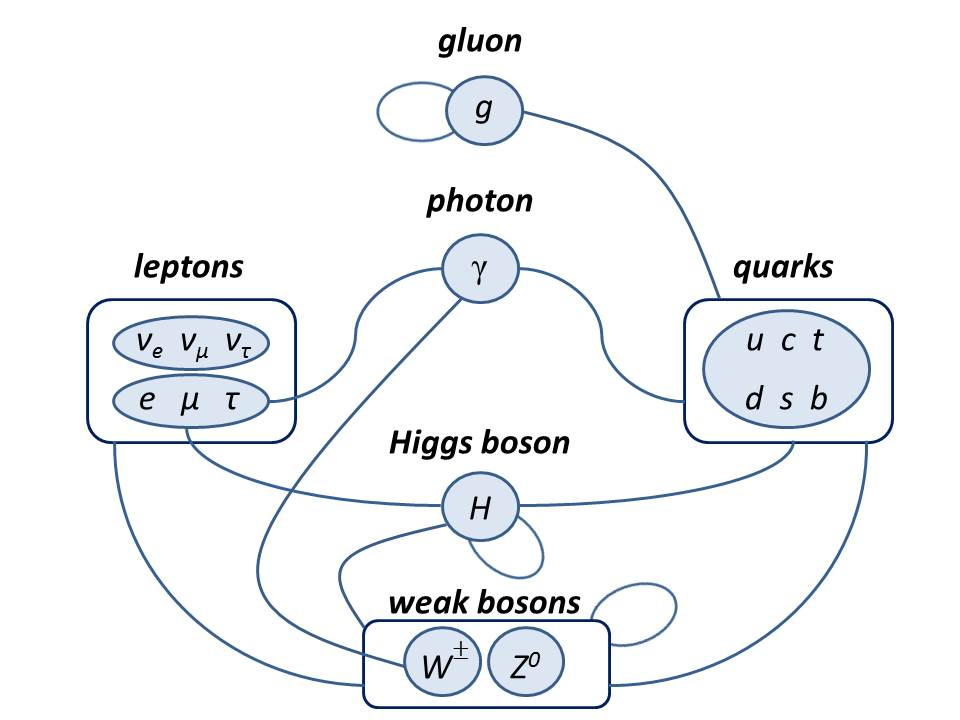
\includegraphics[width=0.85\textwidth]{figures/SM.jpg}
  \end{tabular}
  \caption{Overview of particles contained in the standard model. Blue lines indicate interactions between different particles.}
  \label{fig:SM}
\end{figure}
\\
Mathematically, the standard model is a quantum field theory in which interactions between particles are described via gauge symmetries. The underlying gauge group of the standard model is 
\begin{equation*}
SU(3)_{C} \otimes SU(2)_{L} \otimes U(1)_{Y} 
\end{equation*}
in which $SU(3)$ is the gauge group of the strong force and $C$ indicates that this force acts on the colour charge, $SU(2)$ represents the weak force and $L$ denotes that this force only acts on left-handed fermions while $U(1)$ represents the electromagnetic force acting on the hypercharge $Y$.\\
A brief description of the properties of the particles contained in the SM and the corresponding interactions is given in the following:
\begin{description}

\item \textbf{Matter Constituents:}
In the SM, one distinguishes between twelve different fermions being the elementary constituents of matter. For each fermion there exists also an antiparticle which carries the opposite-signed quantum numbers.
 \begin{description}
  \item \textit{Leptons:} The SM contains, in total, six leptons which are three negatively charged leptons (\lel, \lmu, \ltau) and three neutral leptons (\nue, \numu, \nutau), the neutrinos. In addition to the charge, leptons are also distinguished according to the lepton numbers which are electron number $L_{\lel} = 1$ for electron and electron-neutrino, muon number $L_{\lmu} = 1$ for muon and muon-neutrino and tauon number $L_{\ltau} = 1$ for tauon and tauon-neutrino. Each pair of lepton and neutrino carrying the same lepton number is arranged in a so-called \textit{generation} where \lel and \nue belong to the first generation, \lmu and \numu to the second and \ltau and \nutau to the third, respectively.
  \item \textit{Quarks:} The remaining six fermions in the SM are quarks and can be grouped into generations analogous to the leptons. The first generation comprises the up- and down-quark (\qu, \qd), the second the charm- and strange-quark (\qc, \qs) and the third the top- and bottom-quark (\qt, \qb). All quarks carry electrical charge, but in contrast to leptons, it is not integer, but $+2/3$ for the up-type quarks (\qu, \qc, \qt) and $-1/3$ for down-type quarks (\qd, \qs, \qb). Besides to the electrical charge, quarks also carry colour charge which comes in three types.
 \end{description}
In addition to the attributes described above, fermions are furthermore characterized by the weak isospin. In each generation, left-handed fermions form an isospin-doublet with a weak isospin of $\pm 1/2$ while right-handed components are isospin-singlets with a weak isospin of 0. 
\item \textbf{Fundamental Forces:}
Matter particles interact with each other through fundamental forces mediated via gauge bosons. These bosons arise from the principle of local gauge invariance under symmetry transformations. 
 \begin{description}
  \item \textit{Electromagnetic Force:} The description of the electromagnetic force is based on the theory of \textit{Quantum Electrodynamics} (QED). It is exchanged between electrically charged particles, like the charged leptons and quarks, by the exchange of photons. These are massless and electrically neutral resulting in the property that the electromagnetic force is long ranged.
  \item \textit{Weak Force:} The weak force acts on left-handed fermions, \ie on fermions with non-zero weak isospin, and manifests in charged and neutral currents. Weak interactions preferably take place within one fermion generation. However, since the mass eigenstates in the weak interaction differ from the flavour eigenstates, also transitions between different generations are possible. In the quark-sector, typically a representation is chosen in which the up-type flavour eigenstates correspond to the mass eigenstates and the down-type quarks mix. This mixing is described by the CKM-matrix ~\cite{PhysRevLett.10.531, PTP.49.652}. This is a unitary matrix, described by three mixing angles and one CP-violating phase, which indicates the relative strength between individual transitions. Similarly, also in the neutrino sector a mixing between the weak and the mass eigenstates occurs which leads to the phenomenom of \textit{neutrino oscillation}~\cite{Maki:1962mu, Pontecorvo:1967fh, Fukuda:1998mi}.
  \item \textit{Strong Force:} The theoretical framework describing the strong force is called Quantum Chromodynamics (QCD). It is mediated via eight massless gluons and acts on the colour charge which is carried for instance by quarks. In contrast to the photon, which is electrically neutral and thus can not interact with itself, gluons carry a colour charge and hence couple to themselves. The colour charge exists in three different states commonly denoted as \textit{red}, \textit{green} and \textit{blue}. \\
Regarding the dependence on the distance, the strong force behaves differently than other fundamental forces: the coupling strength increases with rising distance. This is a consequence of the different colour states and the self-coupling property of gluons. It is referred to as \textit{confinement}~\cite{Alkofer:2006fu} and describes the fact that coloured objects can not exist freely. Actually, when separated, coloured objects start to build new coloured particles until only a colour neutral formation is left. Such colourless objects linked by the strong force are named \textit{hadrons}. On the other hand, particles taking part in the strong interaction start to behave quasi-free, \ie the coupling strength is small, when the distance decreases. This feature is known as \textit{asymptotic freedom}~\cite{PhysRevLett.30.1346, PhysRevLett.30.1343}. \\
A typical example for a hadron is the proton. In a simplified picture, it is composed of three quarks: two up quarks and one down quark (\textit{valence quarks}). However, the valence quarks continuously exchange gluons which can exchange further gluons or split into quark-antiquark pairs (\textit{sea quarks}). The constituents of the proton are commonly denoted \textit{partons} and the internal proton structure is described by \textit{parton-distribution functions} (PDFs) specifying the momentum fraction of the proton carried by individual partons.
 \end{description}
First proposed by Salam, Glashow and Weinberg~\cite{Glashow:1961tr, Weinberg:1967tq}, the electromagnetic and the weak force could be successfully unified into the electroweak force. As denoted earlier, the weak force acts on the weak isospin $T_{3}$ while the electromagnetic force acts on the hypercharge $Y$. These two quantities are connected via the following relation to the electric charge $Q$
\begin{equation*}
Q = T_{3} + Y/2 \; .
\end{equation*}
In the electroweak theory, three gauge bosons $W^{1,2,3}_{\mu}$ are introduced for $SU(2)_{L}$ and one gauge boson $B_{\mu}$ for $U(1)_{Y}$. The physical states photon, \Wpm and \Z boson are formed by mixing of these massless states. While the charged $\Wpm$ bosons are superpositions of $W^{1}_{\mu}$ and $W^{2}_{\mu}$, the fields $A_{\mu}$ of the photon and $Z_{\mu}$ of the neutral vector boson are obtained by a mixing of the gauge fields $W^{3}_{\mu}$ and $B_{\mu}$ according to
\begin{equation}
\left(
\begin{matrix}
A_{\mu} \\ Z_{\mu}
\end{matrix}
\right)
=
\left(
\begin{matrix}
\mathrm{cos} \, \theta_{W} & \mathrm{sin} \, \theta_{W} \\
-\mathrm{sin} \, \theta_{W} & \mathrm{cos} \, \theta_{W}
\end{matrix}
\right)
\left(
\begin{matrix}
 B_{\mu} \\ W^{3}_{\mu} 
\end{matrix}
\right)
\end{equation}
with the weak mixing angle $\theta_{W}$. This mixing angle relates also the electromagnetic coupling strength $e$ and the weak coupling strength $g$ according to
\begin{equation}
e = g \, \mathrm{sin} \, \theta_{W} \; .
\end{equation}
The fields $W^{\mu}$ couple only to left-handed fermions such that the same holds also for $W^{\pm}$. Since, however, the $B^{\mu}$ couples to left- and right-handed states, a coupling to left- and right-handed fermions takes place for $\gamma$ and $Z^0$. Unlike the photon, the $W^{\pm}$ and $Z$ vector bosons are massive with masses\footnote{In this thesis, natural units are used, \ie $\hbar = c =1$. Thus, also particle masses and momenta have the dimension of energies.} of $\Wpm = 80.385 \pm 0.015$\gev and $\Z = 91.1876 \pm 0.0021$\gev~\cite{Agashe:2014kda}. As a result, the weak interaction is suppressed with respect to the electromagnetic force. 
\item \textbf{Higgs Boson:} The electroweak theory in the current representation requires that fermions and bosons are massless particles as mass terms violate the gauge invariance under $SU(2)_{L} \otimes U(1)_{Y}$ transformations. This is in contradiction to experimental observations which have shown that all particles, except for photon and gluon, in fact do have mass. \\
An explanation for the generation of particle masses without violation of the principles of the electroweak theory is provided by the \textit{Higgs-mechanism}~\cite{PhysRevLett.13.508, PhysRevLett.13.321, PhysRevLett.13.585} which is based on the concept of spontaneous symmetry breaking. The main idea behind this meachnism is that while in general the principle of local gauge invariance is obeyed, it is explicitly broken by the ground state. \\
In the context of the Higgs-mechanism, this is realized by the introduction of the Higgs field $\Phi$ described by a potential 
\begin{equation*}
\mathcal{V}(\Phi) = \mu^2 \Phi^+\Phi^- \, + \, \lambda (\Phi^+\Phi^-)^2
\end{equation*}
with parameters $\mu$ and $\lambda$. Choosing $\mu^2$ to be negative and $\lambda$ positive, the potential has a non-zero minimum value with the vacuum expectation value
\begin{equation*}
v = \sqrt{\frac{-\mu^2}{2\lambda}} \; .
\end{equation*}
Expansion of the Higgs field around this vacuum expectation value eventually leads to a new spin-0 particle, the scalar \textit{Higgs boson}, which is a quantum excitation of one of the components of the Higgs field. Furthermore, the masses of gauge bosons are generated by the couplings to the Higgs field according to
\begin{equation*}
m_{\gamma} = 0, \;\;\; m_W = \frac{v}{2}g, \;\;\; m_Z = \frac{m_W}{\mathrm{cos}\theta_{W}}, \;\;\; m_H = \sqrt{-2\mu^2} \;.
\end{equation*}
Similarly, the Higgs mechanism introduces mass terms for fermions 
\begin{equation*}
m_{f} = G \frac{v}{\sqrt{2}}
\end{equation*}
resulting from Yukawa couplings to the Higgs field with coupling constants $G_i$. \\
The discovery of a new boson at a mass of around 125\gev has been announced by the ATLAS and CMS collaborations in 2012~\cite{Aad:2012tfa, Chatrchyan:2012ufa}. As all properties of this new boson are consistent with SM predictions for the Higgs boson so far (\cf for instance~\cite{Aad:2013wqa, Aad:2014eva, Aad:2014eha, CMS-PAS-HIG-14-009}), this indicates that the last remaining gap of the SM could finally be closed.   
\end{description}

\subsection{Limitations of the Standard Model}
\label{subsec:sm_shortcomings}
Although the SM has been very successful so far leading to several discoveries while withstanding numerous precision tests, it is known to be an incomplete theory. Some of the shortcomings of the SM are:
\begin{description}
\item \textbf{Gravity:} As stated already earlier, the SM contains no description of gravity. In particular, it is currently not possible to unify general relativity and quantum theory in one common concept.
\item \textbf{Matter-antimatter asymmetry:} According to the SM, matter and anitmatter exist to equal amounts in the universe which is in fact not the case. A theory, which would be able to explain the observed asymmetry, needs some source of $CP$-violation. The only source of $CP$-violation within the SM is arising from the CKM matrix as described in~\ref{sec:sm}. However, this is not enough to be able to explain the degree of matter-antimatter asymmetry in the universe~\cite{bib:CPViolation}.    
\item \textbf{Unification of couplings:} The unification of the electromagnetic and the weak force leads to the question if it is possible to further unify the electroweak force with the strong force in order to build a combined theory, usually referred to as Grand Unified Theory (GUT). This would require that the coupling constants of the SM intersect when extrapolating them from the electroweak to the GUT scale. However, this feature is not observed within the SM.
\item \textbf{Nature of dark matter:} There exist several cosmological observations that indicate that the matter described by the SM makes up only $4.9$\% of the universe~\cite{Ade:2013zuv}. A by far larger part of $26.8$\% is assigned to so-called \textit{dark matter} which is presumably neutral and only weakly interacting. The only particles within the SM possessing such attributes are neutrinos. However, they are not able to account for the whole relic density present in the universe~\cite{Bertone:2004pz}. 
\item \textbf{Hierarchy problem:} The observable mass of the Higgs boson is given by the bare mass of the Higgs boson plus contributions arising from higher order corrections caused by each massive SM particle. For a fermion with mass $m_f$ and Yukawa coupling $\lambda_f$ to the Higgs field, the corrections to $m_H^2$ are
\begin{equation}
\label{eq:hierarchy}
\Delta m_H^2 \propto -\frac{|\lambda_f|^2}{8\pi^2}\Lambda_\mathrm{UV}^2 \propto m_f^2
\end{equation}
 with an ultraviolet cut-off scale $\Lambda_\mathrm{UV}$. Typically, this cut-off scale is interpreted as the energy at which new physics enter. If it is chosen to be the Planck scale, the Higgs mass is several orders of magnitudes larger than the electroweak scale and thus would require an enormous amount of fine-tuning at each order of perturbation theory to yield the expected Higgs mass around $\mathcal{O}(100)$\gev. 
\end{description} 

\section{Supersymmetry}
\label{sec:susy}
In order to overcome the weaknesses of the SM and to provide explanations for so far unsolved problems, several theories have been developed which go beyond the SM. Among those, a favoured extension is \textit{supersymmetry} (SUSY) as it is able to provide several benefits at once. The first supersymmetric four-dimensional quantum field theory has been introduced by Wess and Zumino in 1974~\cite{bib:WessZumino}. \\
In this section, a brief introduction to the general concept of supersymmetry is given with focus on the \textit{Minimal Supersymmetric Standard Model} (MSSM). For detailed reviews see, \eg\cite{Aitchison:2005cf, Martin:1997ns}.\\ 
\\
%The basic idea behind supersymmetry is that each standard model particle gets a supersymmetric partner particle which possesses the same quantum numbers except for the spin which differs by $1/2$. 
The basic idea of a supersymmetric theory is that a fermionic state is converted into a bosonic state and vice versa by the generator of a supersymmetry transformation $Q$ according to
\begin{equation*}
Q \ket{\mathrm{fermion}} \, = \, Q \ket{\mathrm{boson}}, \hspace{20mm} Q \ket{\mathrm{boson}} \, = \, Q \ket{\mathrm{fermion}}.
\end{equation*}
The supersymmetric fermionic and bosonic partner particles are called \textit{superpartners} and form together the irreducible representations of the supersymmetry algebra named \textit{supermultiplets} with the same number of fermionic and bosonic degrees of freedom. In case of unbroken supersymmetry, partner particles within one supermultiplet have the same mass as well as the same quantum numbers, like electric charge, weak isospin and colour degrees of freedom, except for the spin. Commonly, supersymmetric particles are denoted \textit{sparticles}. \\
\\
In a general supersymmetric theory fulfilling the criteria of gauge invariance and renormalisability, processes are allowed which violate either lepton or baryon number conservation. However, a baryon and lepton number violation would imply for instance a rapid decay of protons. The lower limit on the proton lifetime is found to be $5.9 \times 10^{33}$ years at 90\% confidence level~\cite{PhysRevD.90.072005} and indicates that such processes must be suppressed. In order to achieve this, a new quantum number called \textit{R-parity} is introduced according to  
\begin{equation*}
R = (-1)^{3(B-L) + 2S}
\end{equation*}
with baryon number $B$, lepton number $L$ and spin $S$. It is a multiplicative quantum number and amounts to $R= +1$ for SM particles while it is $R = -1$ for supersymmetric particles. Assuming $R$-parity conservation, no baryon or lepton number violation processes occur.\footnote{There exist also several $R$-parity violating SUSY models which are not in contradiction to the observed proton lifetime (\cf for instance~\cite{Martin:1997ns}). However, these models are not subject of this thesis and thus not discussed.} In addition, the assumption of $R$-parity conservation leads to further phenomenological implications:
\begin{itemize}
\item SUSY particles can only be produced in pairs at collider experiments as only even numbers of supersymmetric particles can occur at an interaction vertex.
\item The lightest supersymmetric particle (LSP) is stable and thus any decay chain of a supersymmetric particle finally ends in a state containing an odd number of LSPs.
\end{itemize}
A $R$-parity conserving supersymmetric theory provides some elegant solutions to open questions as raised in Sec.~\ref{subsec:sm_shortcomings}:
\begin{itemize}
 \item The Higgs mass suffers from quadratically divergent contributions arising from higher-order corrections caused by SM particles. However, since in SUSY each SM particle gets a supersymmetric partner, these higher order corrections cancel. For instance for the fermion contributions described in Eq.~\ref{eq:hierarchy}, the quadratically divergent terms are canceled by contributions with opposite sign that arise from a scalar with same mass and thus the same coupling strength to the Higgs field. Since the same cancelation occurs for bosons vice versa, SUSY is able to provide a solution to the hierarchy problem. However, no observation of such kind of supersymmetric particles with exact same masses as their SM correpondents has been made such that supersymmetry in fact has to be a broken symmetry. In order to still be able to provide a solution to the hierarchy problem, supersymmetric particles are expected to be not heavier than $\mathcal{O}(\mathrm{1\tev})$, which is typically referred to as \textit{natural supersymmetry}. This is the main argument why one would expect masses of supersymmetric particles to be in the TeV range, well within the reach of the LHC. Some more considerations about natural SUSY follow in Sec.~\ref{subsec:natural_susy}.
 \item Considering the existence of low scale supersymmetric particles, the coupling constants of the forces meet in one point when extrapolating the couplings from the electroweak to the GUT scale. This effect is illustrated in Fig.~\ref{fig:couplings}. It is visible that the evolution of the couplings is modified with respect to the SM at that energy scale where the supersymmetric particles enter. In general, this hints to the possibility of a grand unification.
\begin{figure}[!t]
  \centering
  \begin{tabular}{c}
    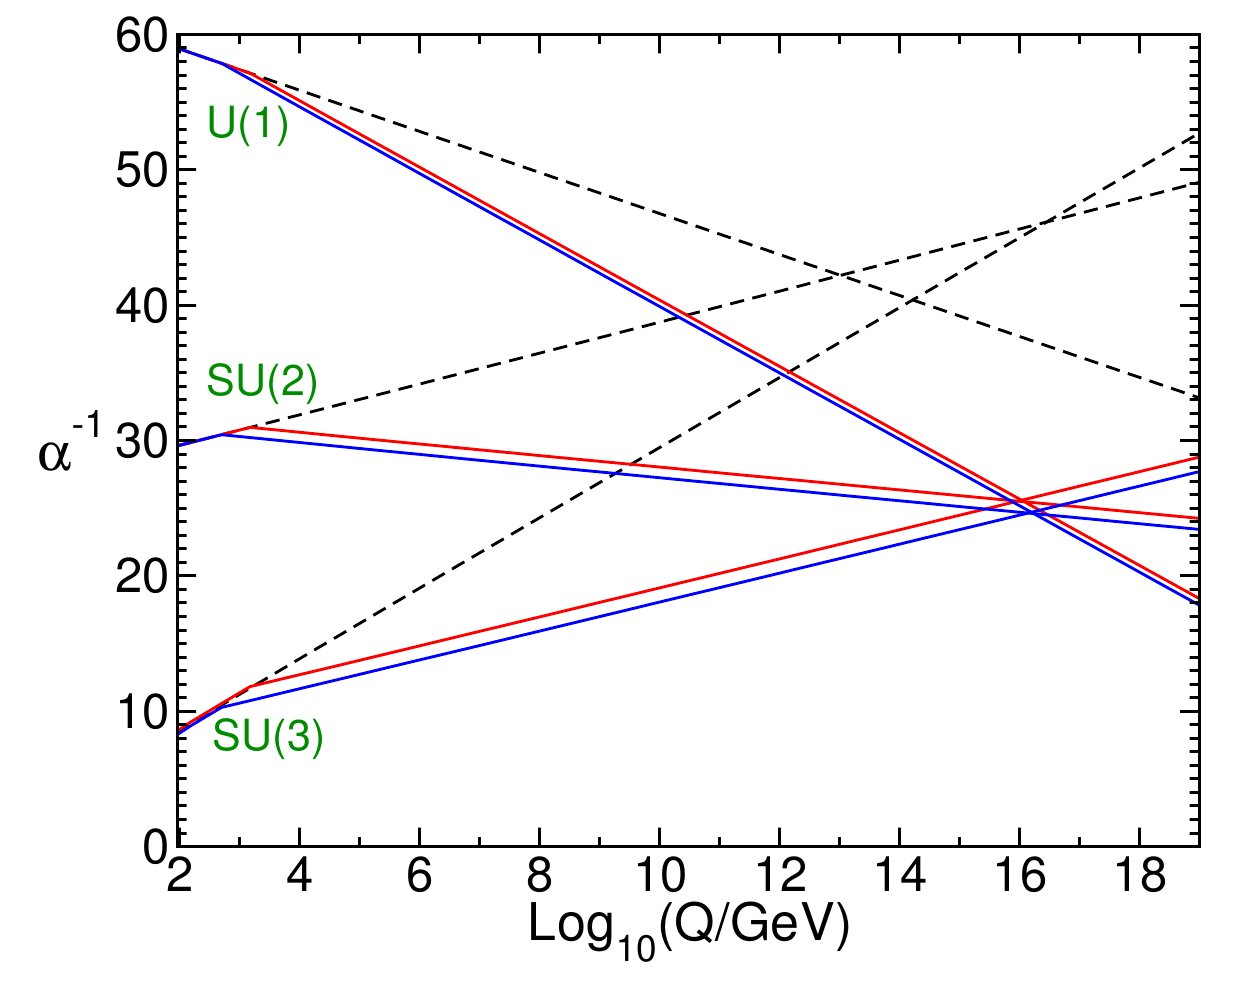
\includegraphics[width=0.55\textwidth]{figures/Couplings.jpg}
  \end{tabular}
  \caption{Comparison of the renormalization group evolution of the couplings $\alpha_{a}^{-1}$ in the SM (dashed lines) and the MSSM (solid lines) including two-loop effects. The masses of the supersymmetric particles in the MSSM are considered as a common threshold changing between 500\gev and 1.5\tev while the strong coupling constant $\alpha_{3}(m_{Z})$ is varied between 0.117 and 0.121. Taken from~\cite{Martin:1997ns}.}
  \label{fig:couplings}
\end{figure}
 \item $R$-parity conserving SUSY models provide a suitable dark matter candidate. As discussed previously, each decay of supersymmetric particles finally leads to the existence of an LSP which is stable. Thus, it is an adequate DM candidate when it is only weakly interacting.
 \item Supersymmetry is in principal also suited to explain the observed matter-antimatter asymmetry in the universe as especially the description of supersymmetry breaking can involve $CP$-violating phases. However, these phases are strongly constraint by experimental results (\cf for instance~\cite{Ibrahim:2007fb} for a comprehensive review).
 \item SUSY might also provide an indication of the nature of gravity. As denoted in Sec.~\ref{subsec:sm_shortcomings}, it is currently not possible to unify general relativity and quantum theory. However, supersymmetry is a crucial requirement for \textit{string theories} which are the only suited candidates for a quantum field theory of gravity to date (see, \eg\cite{RevModPhys.47.123}). 
\end{itemize} 

\subsection{Natural Supersymmetry}
\label{subsec:natural_susy}
As introduced above, SUSY models are considered natural if they provide a solution to the hierarchy problem. Commonly, certain measures are introduced to estimate the naturalness of a supersymmetric model. \\
One example is the Veltman definition of naturalness~\cite{veltman1981infrared}. This states that radiative contributions should not exceed tree-level effects in size, regarding the mass of a scalar particle. Another definition is given by Babieri and Giudice~\cite{Barbieri198863} which do not restrict the magnitude of the radiative corrections, but the sensitivity of the physical mass of a scalar $m$ to small changes in the bare couplings $\lambda_0$. This constraint is often imposed by quantifying the amount of necessary fine-tuning $\Delta$ according to
\begin{equation}
\left| \frac{\lambda_0}{m^2}\frac{\partial m^2}{\partial \lambda_0} \right| < \Delta \; .
\end{equation}
While the value of $\Delta$ has been set to $\sim10$ in the past, it increased over the years such that also values of $\sim100$ or even $\sim1000$ are often considered as reasonable values~\cite{Craig:2013cxa}. \\
Such conditions can be used in order to derive constraints on the spectrum of superpartners which regulate the hierarchy problem. Here, it turns out that not all sparticles are equally important and thus not all have to be situated at the same mass scale. Some typical mass ranges for sparticles considered as natural are given in Sec.~\ref{subsec:mssm}. 

\subsection{The MSSM}
\label{subsec:mssm}
In general, it is possible to have theories with more than one supersymmetry transformation $N$. However, the smallest possible supersymmetric extension of the SM including the full particle spectrum and interactions, \ie a $N = 1$ supersymmetry, is realised in the MSSM. An overview of the respective particle content is given in Tab.~\ref{tab:particle_content}. 
\begin{table}[!t] 
  \centering
%   \makebox[\linewidth]{
    \begin{tabular}{cccc}
%      \hline
      \toprule
      Type & Spin & Gauge eigenstates & Mass eigenstates \\
      \midrule
      \midrule
      Higgs bosons & 0 & $H_{u}^{0}$ $H_{d}^{0}$ $H_{u}^{+}$ $H_{d}^{-}$ & $h^{0}$ $H^{0}$ $A^{0}$ $H^{\pm}$  \\
      \midrule
      & & $\tilde{u}_{L}$ $\tilde{u}_{R}$ $\tilde{d}_{L}$ $\tilde{d}_{R}$ &  see left \\
      Squarks & 0 & $\tilde{s}_{L}$ $\tilde{s}_{R}$ $\tilde{c}_{L}$ $\tilde{c}_{R}$  & see left \\
      & & $\tilde{t}_{L}$ $\tilde{t}_{R}$ $\tilde{b}_{L}$ $\tilde{b}_{R}$ & $\tilde{t}_{1}$ $\tilde{t}_{2}$ $\tilde{b}_{1}$ $\tilde{b}_{2}$ \\
      \midrule
      & & $\tilde{e}_{L}$ $\tilde{e}_{R}$ $\tilde{\nu}_{e}$ &  see left \\
      Sleptons  & 0 & $\tilde{\mu}_{L}$ $\tilde{\mu}_{R}$ $\tilde{\nu}_{\mu}$ & see left \\
      & & $\tilde{\tau}_{L}$ $\tilde{\tau}_{R}$ $\tilde{\nu}_{\tau}$ & $\tilde{\tau_{1}}$ $\tilde{\tau_{2}}$ $\tilde{\nu_{\tau}}$ \\
      \midrule
      Neutralinos  & 1/2 & $\tilde{B}^{0}$ $\tilde{W}^{0}$ $\tilde{H}_{u}^{0}$ $\tilde{H}_{d}^{0}$ & $\tilde{\chi}_{1}^{0}$ $\tilde{\chi}_{2}^{0}$ $\tilde{\chi}_{3}^{0}$ $\tilde{\chi}_{4}^{0}$ \\
      \midrule
      Charginos & 1/2 & $\tilde{W}^{\pm}$ $\tilde{H}_{u}^{+}$ $\tilde{H}_{d}^{-}$ & $\tilde{\chi}_{1}^{\pm}$ $\tilde{\chi}_{2}^{\pm}$ \\
      \midrule
      Gluino & 1/2 & $\tilde{g}$ & see left \\
      \midrule
      Gravitino & 3/2 & $\tilde{G}$ & see left \\
      \bottomrule
    \end{tabular}%}
 \caption{Supersymmetric particles contained in the MSSM neglecting mixing in the first two sfermion generations. Adapted from~\cite{Martin:1997ns}.} 
  \label{tab:particle_content}
\end{table}
This extension is minimal in the sense that it introduces the least feasible number of additional particles to the existing SM particles meaning that each SM fermion gets one superpartner. The interactions and couplings of the supersymmetric particles are the same as for the SM counterparts. The different transformation of left- and right-handed fermions under the gauge groups implies the necessity to introduce separate superpartners for left- and right-handed states as well. These are arranged with their bosonic (spin 0) superpartner in a \textit{chiral} supermultiplet. The labels indicating the left- and right-handed states refer to the helicity of the respective SM particle. These supersymmetric partners of fermions are named \textit{sfermions} distinguishing between \textit{sleptons} and \textit{squarks}, the supersymmetric partners of leptons and quarks. In a similar manner, the SM gauge bosons are arranged in \textit{gauge} supermultiplets together with their fermionic (spin 1/2) supersymmetric correspondents. The SUSY partners of the gauge bosons are named \textit{gauginos} so that the superpartners in the gauge supermultiplets are the \textit{gluino}, \textit{wino} and \textit{bino}. The corresponding gaugino mixtures of the neutral wino and the bino are the \textit{photino} and the \textit{zino}. Furthermore, the supersymmetric particle spectrum is extended by another supermultiplet containing the graviton (spin 2) and the respective supersymmetric partner -- the \textit{gravitino} (spin 3/2). \\
As described in Sec.~\ref{sec:sm}, masses arise in the SM from the concept of spontaneous symmetry breaking implying the existence of the Higgs boson. The supersymmetric partner of the Higgs boson is named \textit{higgsino}. While in the SM one Higgs doublet is sufficient to give mass to all particles, the Higgs sector needs to be extended in the MSSM. Here, two Higgs doublets are needed with one doublet $H_u$ giving mass to the up-type quarks and the other one $H_d$ to the down-type quarks, respectively. These two doublets have together eight degrees of freedom of which three are needed to give mass to the gauge bosons of the weak interaction as in the SM. This results in five physical Higgs bosons which are the two scalar Higgs particles $h^0, H^0$, the pseudoscalar $A^0$ as well as the charged Higgs bosons $H^{\pm}$. As further consequence, there are two vacuum expectation values $v_u$ and $v_d$ present, each assigned to one Higgs doublet, whose ratio $\mathrm{tan} \, \beta = v_u/v_d$ is a free parameter of the model. Within the MSSM, the mass of the lightest Higgs boson is restricted to be smaller than the $Z$-boson mass at tree level. However, due to radiative corrections, which mainly arise from the top sector, this limit is enhanced and results in an upper bound of~\cite{Martin:1997ns} 
\begin{equation*}
m_{h^0} \lesssim 135 \gev \; .
\end{equation*}
Consequently, significant contributions from the stop quark mass are required to push the mass of the lightest Higgs boson up to a value of around 125\gev. This is somewhat in tension to the requirement of having a stop quark mass close to the top mass in order to solve the hierarchy problem. However, it is still possible to accommodate a Higgs mass of 125\gev without the necessity to decouple the stop quark or add new dynamics to the MSSM. These scenarios are referred to as \textit{maximal mixing}~\cite{Djouadi:2005gj}. \\
Similar to the SM, the gauge eigenstates of the SUSY theory are not necessarily equal to the mass eigenstates. A mixing occurs especially in the gaugino sector. Here, the neutral components of the bino and wino mix with the neutral higgsinos and form four mass eigenstates called \textit{neutralinos} $\tilde{\chi}^0$. Similarly, also the charged gauginos and higgsinos mix to the four \textit{charginos} $\tilde{\chi}^{\pm}$. Furthermore, mixing can also appear in the third squark and slepton generation. The mixing is supposed to be significant only for fermions of the third generation as the off-diagonal elements of the sfermion mass matrix are proportional to the mass of the respective SM partner. \\
In order to obtain a natural realization of the MSSM, it is important that certain particles have a particular mass scale~\cite{Craig:2013cxa}. Especially the superpartner of the top quark is expected to be not too heavy in order to be able to cancel the contributions from top loops to the Higgs mass. These give typically the largest contributions since the top quark is the heaviest particle in the SM. Assuming a maximal accepted fine-tuning of $\Delta \lesssim 10$, the stop mass is supposed to be around 400\gev. Given these conditions, also light higgsinos are expected with a typical mass scale around 200\gev. Since gluinos yield loop corrections to the stop mass, they are expected to not significantly exceed the 1\tev range as a second order effect. 

\subsection{SUSY-Breaking}
\label{subsec:susy_breaking}
\begin{figure}[!t]
  \centering 
  \begin{tabular}{c}
    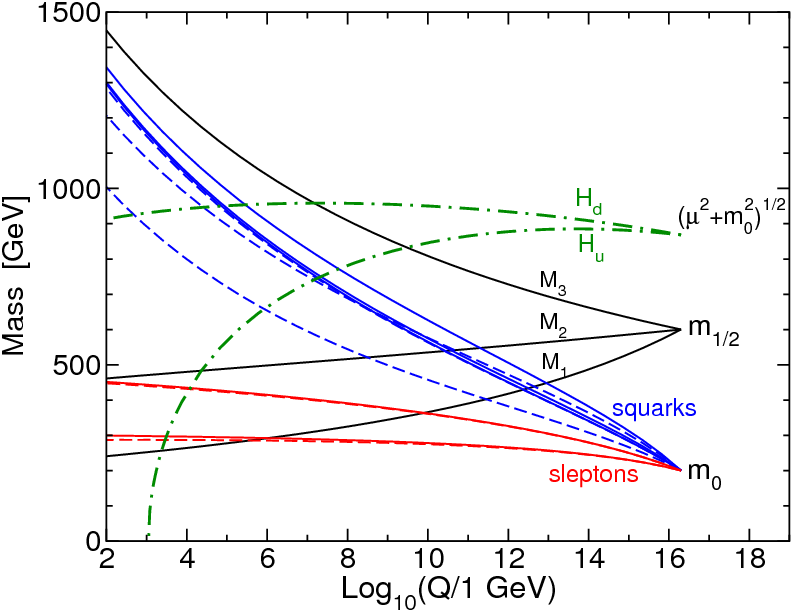
\includegraphics[width=0.6\textwidth]{figures/MSSMrun.png}
  \end{tabular}
  \caption{Evolution of scalar and gaugino mass parameters in the MSSM with mSUGRA boundary conditions imposed at $Q_0 = 2 \times 10^{16}$\gev. The parameter $\mu^2 + m^2_{H_{u}}$ runs negative, provoking electroweak symmetry breaking~\cite{Martin:1997ns}.}
  \label{fig:MSSMrun}
\end{figure}
As discussed above, SUSY particles are in general expected to have the same mass as their corresponding SM partner particle. Since, however, none of such particles has been observed so far, this implies that supersymmetry in fact must be broken and that sparticles are actually heavier than the SM counterparts. \\%If SUSY is expected to provide a solution to the hierarchy problem, the mass difference to the SM particles should consequently not be too large and the characteristic mass scale needs to be around 1\tev~\cite{Martin:1997ns}. \\
Typically, SUSY breaking is introduced such that so-called \textit{soft breaking} terms, \ie of positive mass dimension, are added to the theory in addition to the terms determining the gauge and Yukawa couplings. The SUSY breaking is assumed to take place in a hidden sector which does not couple directly to the visible sector represented by the supermultiplets. In this case, no specific breaking mechanism must be assumed, but only a mechanism to describe the mediation of the supersymmetry breaking from the hidden to the visible sector. In total, the MSSM, including soft SUSY breaking, features several new phases, mixing angles and masses which add another 105 free parameters to the already existing parameters of the SM~\cite{Dimopoulos:1995ju}.  \\
Two SUSY breaking scenarios, that are often studied, are either based on gravity-mediated or gauge-mediated interactions and known as \textit{minimal supergravity} (mSUGRA)~\cite{Chamseddine:1982jx, AlvarezGaume:1983gj} or \textit{constrained MSSM} (CMSSM)~\cite{Kane:1993td, Baer:2002gm} and \textit{gauge-mediated supersymmetry breaking} (GMSB)~\cite{Dine:1981gu, AlvarezGaume:1981wy}. Assuming a specific breaking scenario usually allows to drastically reduce the number of free parameters in the theory and determines the phenomenology of the respective model. In case of mSUGRA/CMSSM, the whole model can be described by five parameters, which are the common scalar mass $m_0$ and the common mass of the gauginos and higgsinos $m_{1/2}$ at the GUT scale, the common trilinear coupling $A_0$, $\mathrm{tan} \, \beta = v_u/v_d$ and the sign of the higgsino mass parameter $\mu$. In Fig.~\ref{fig:MSSMrun}, the evolution of the corresponding mass parameters to the electroweak scale is illustrated.  

\section{Searches for Supersymmetry and Current Constraints}
\label{sec:susy_status}
The appealing attributes of supersymmetry, which have been discussed above, initiated a couple of indirect and direct searches looking for hints of supersymmetric particles. Although no sign for SUSY has been observed in nature so far, several results have been used in order to constrain the allowed parameter space. %%%%%This section gives a short introduction to general search strategies for supersymmetry with main focus on collider experiments and provides a short overview of the status of experimental results. Results of direct searches at the LHC discussed in this section are restricted to results from searches performed previous to the analysis presented in this thesis. Further discussion of the status of supersymmetry after LHC Run-I follows in Sec.~\ref{sec:susy_status}.  

\subsection{Indirect Constraints}
\label{subsec:susy_indirect}
The existence of supersymmetric particles can show up in manifold ways. For instance, higher-order contributions to SM processes could be induced from SUSY. Such contributions might impact for instance electroweak precision data, rare decays of $B$ mesons or the anomalous magnetic moment of the muon. However, global fits to electroweak precision data using several precision measurements of SM parameters and particle masses, like $m_W$ and $m_t$, together with theoretical calculations have found no evidence for any inconsistency of the SM-only hypothesis so far~\cite{LEP-2, Erler:2012wz, Ciuchini:2013pca, Baak:2014ora}. Furthermore, precise measurements of rare processes in $B$-meson decays, like $B_s^0 \rightarrow \mu^+ \mu^-$, are in good agreement with expectations from the SM~\cite{Chatrchyan:2013bka, Aaij:2013aka, CMS-PAS-BPH-13-007}. The most compelling difference between experimental results and SM prediction is currently observed for the anomalous magnetic moment of the muon~\cite{Bennett:2006fi, Hagiwara:2011af, Agashe:2014kda}. Here, deviations at the level of $3.6\sigma$ occur. However, discussions about the accuracy of the SM calculation are ongoing~\cite{Davier:2010nc}. \\  
Further constraints arise from astrophysical and cosmological studies. Several observations suggest that a considerable amount of cold dark matter contributes to the composition of the universe~\cite{wmap, Ade:2013zuv}. Good candidates are weakly interacting massive particles (WIMPs) which could be the neutralino in SUSY models where it is the LSP. Consequently, also the observed cold dark matter relic density can put constraints on the MSSM parameter space assuming that it is caused by a neutralino LSP. Thus, constraints on supersymmetry can be derived in particular from direct and indirect dark matter searches (\cf for instance~\cite{cerdeno2010direct, Cirelli:2010xx, PhysRevLett.109.181301, Ackermann:2013uma, Agnese:2013jaa, Angloher:2014myn, PhysRevLett.113.121101, Abramowski:2014tra}). 

\subsection{Searches at pre-LHC Collider Experiments}
\label{subsec:susy_collider_pre-lhc}
Although the exploitation of indirect searches for supersymmetry is very useful in order to constrain the allowed SUSY parameter space, the most stringent exclusion limits are derived from direct searches at collider experiments. Typically, searches for SUSY at colliders make use of the specific production and decay properties assuming $R$-parity conservation. As discussed in Sec.~\ref{sec:susy}, $R$-parity conservation implies that sparticles are only produced in pairs and decay via cascades into the lightest supersymmetric particle which is often assumed to be the lightest neutralino. This leaves the experiment undetected and manifests in missing energy or missing momentum. Such missing energy signatures are thus a key-feature of searches for supersymmetry in collider experiments. Depending on the type of supersymmetric particle produced, the missing energy can be accompanied by several leptons, photons or jets. Usually, searches are classified according to their targeted final state and aim at a specific kind of supersymmetric particle. If searches are designed to be sensitive to various types of particles and models, they are called \textit{inclusive} searches. \\  
Extensive searches resulting in the tightest exclusion limits in the pre-LHC era have been realised by the experiments performed at \hera, \lep and \tevatron.

\subsubsection*{HERA}
The main focus of SUSY searches at \hera has been on $R$-parity violating models~\cite{Aktas:2004ij, Aktas:2004tm, Zeus:2006je}. However, also searches for $R$-parity conserving supersymmetric models have been performed~\cite{Aid:1996es, Breitweg:1998gk} and in these models the excluded region extends to around 60--70\gev for squark masses and around 40\gev for the LSP mass, depending on the specific assumptions made to contrain the MSSM parameter space. % processes involving the production of a selectron and a squark. The dominant MSSM process at \hera is the production of a selectron and a squark via the exchange of a neutralino where $\tilde{e}$ and $\tilde{q}$ subsequently decay into any lighter gaugino and their respective SM partner. Thus, a distinct experimental signature is given by an electron, hadrons and missing energy and momentum. Since no excess of such events over the SM expectation has been observed, exclusion limits for the masses of the selectron and squark in the context of the MSSM have been derived. Depending on the specific assumptions made to contrain the MSSM parameter space, the excluded region extends to around 60--70\gev for squark masses and around 40\gev for the LSP mass~\cite{Aid:1996es, Breitweg:1998gk}. \\

\subsubsection*{LEP}
At \lep, various searches for supersymmetry were performed targeting different species of supersymmetric particles in $R$-parity conserving models~\cite{LEPLimits}. Scalar leptons and quarks are mainly pair-produced in the $s$-channel via $Z$ bosons and photons. In case of selectrons, also the $t$-channel exchange of neutralinos yields important contributions. The energy scale at \lep opens a parameter space where sparticles with quite high masses are produced such that they predominantly decay into the respective SM partner particles (except for the scalar top, since the top quark is too heavy) and the lightest neutralino. Furthermore, also cascade decays are possible. Typical final states contain missing energy and a pair of acoplanar leptons (jets) where the direction of the first lepton (jet) is not in the plane defined by the direction of the second lepton (jet) and the beam direction. \\
Similarly, neutralinos and charginos are expected to be pair-produced via $Z/\gamma$ $s$-channel exchange or $t$-channel selectron or sneutrino exchange, respectively. Typically, charginos decay into $\tilde{\chi}_{1}^{0}l\nu$ or $\tilde{\chi}_{1}^{0} qq'$ while in neutralino pairs ($\tilde{\chi}_{1}^{0}\tilde{\chi}_{2}^{0}$) the $\tilde{\chi}_{2}^{0}$ decays into $\tilde{\chi}_{1}^{0} \nu \bar{\nu}, \tilde{\chi}_{1}^{0} l^+ l^-$ or $\tilde{\chi}_{1}^{0} qq'$. Hence, the final state in case of chargino production is characterized by missing energy accompanied by four jets, two jets and one lepton or only leptons, depending on the specific decay mode of the chargino while the most important signatures for neutralino production are acoplanar pairs of jets or leptons coming along with large missing momentum. However, the exact decay topologies strongly depend on the particular mass spectrum of the supersymmetric particles so that the above mentioned topologies could also be accompanied by photons or manifest in multiple jets or leptons in cascade decays. \\
Interpretations of combined results from all four experiments in the mSUGRA model lead to exclusion limits showing that $m_{1/2}$ has to be greater than about 100--200\gev over a range of $m_{0}$ up to the\tev-region for specific fixed other parameters. The lower limit on the LSP mass is found to be around 50\gev~\cite{LEPLimits}. 

\subsubsection*{Tevatron} 
The \tevatron accelerator made another SUSY parameter space accessible for searches as the centre-of-mass energy exceeded that of \hera and \lep by at least one order of magnitude. A rich program of supersymmetric searches was enabled covering various final states of different lepton, photon or jet multiplicities. Of special interest is the search for coloured sparticles, like squarks and gluinos, as \tevatron is a hadron collider. The expected decay topologies are very similar to those at the LHC and thus discussed in Sec.~\ref{subsec:susy_LHC_searches}. \\
Results from SUSY searches at the Tevatron have been interpreted in the context of mSUGRA and extended the LEP results in the parameter region of $m_{0} =$ 70--300\gev and $m_{1/2} =$ 125--165\gev. This allows to exclude gluinos below around 280--300\gev for all squark masses and squarks below $380$\gev independent of the gluino mass~\cite{CDFLimits, D0Limits, Abazov200934}. 

\subsection{Searches at the LHC}
\label{subsec:susy_LHC_searches}
The absence of SUSY-like signals at any collider experiment performed previously to the start of the LHC and exclusion limits at the order of a few hundred GeV on sparticle masses activated a variety of searches for supersymmetry at the LHC. These are targeting the various different production and decay modes of supersymmetric partices and can be classified into searches for squarks and gluinos, third generation sfermions and electroweakinos. Of particular interest are searches for coloured particles, as the LHC is, as well as the \tevatron, a hadron collider. In this thesis, searches for supersymmetry are presented that are based on all-jet final states accompanied by missing transverse energy and no leptons. Thus, these so-called \textit{hadronic signatures} are discussed in the following.

\subsubsection*{Production Modes}
\label{subsubsec:susy_prod}
\begin{figure}[!tp]
  \centering 
  \begin{tabular}{cc}
    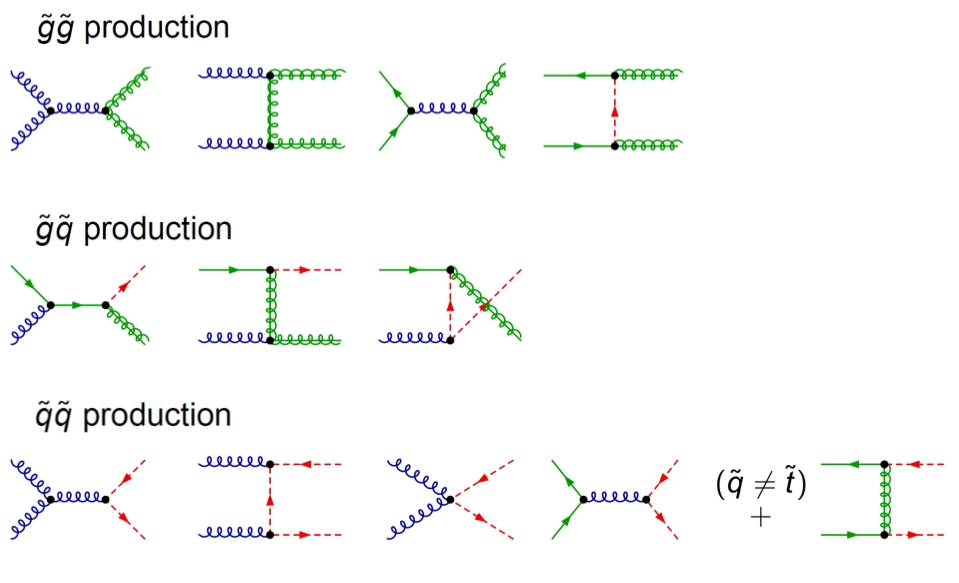
\includegraphics[width=0.8\textwidth]{figures/Susy_Feynman.jpg} 
  \end{tabular}
  \caption{Example diagrams for the production of supersymmetric particles in hadron collisions at parton level.}
  \label{fig:susy_feynman}
\end{figure}
At leading order, sparticles in $R$-parity conserving models are predominantly produced in processes like~\cite{Kane:1982hw, Harrison:1982yi, Reya:1984yz, Dawson:1983fw, Baer:1985xz}
\begin{equation}
 pp \rightarrow \tilde{g}\tilde{g}, \tilde{g}\tilde{q}, \tilde{q}\tilde{q} \, .
\end{equation}
Some example diagrams for the production modes of such processes at parton level are shown in Fig.~\ref{fig:susy_feynman}. Typically, squarks are assumed to be mass-degenerate and refer to the partners of the light-flavour $(u, d, s, c)$ quarks with suppressed chiralities of the squarks $\tilde{q} = (\tilde{q}_L, \tilde{q}_R)$. Supersymmetric partners of the bottom and top quark are considered separately due to a potentially large mixing affecting the mass splitting.
\begin{figure}[!t]
  \centering
  % \makebox[\linewidth]{
  \begin{minipage}[c]{1.\textwidth}
    \begin{center}
      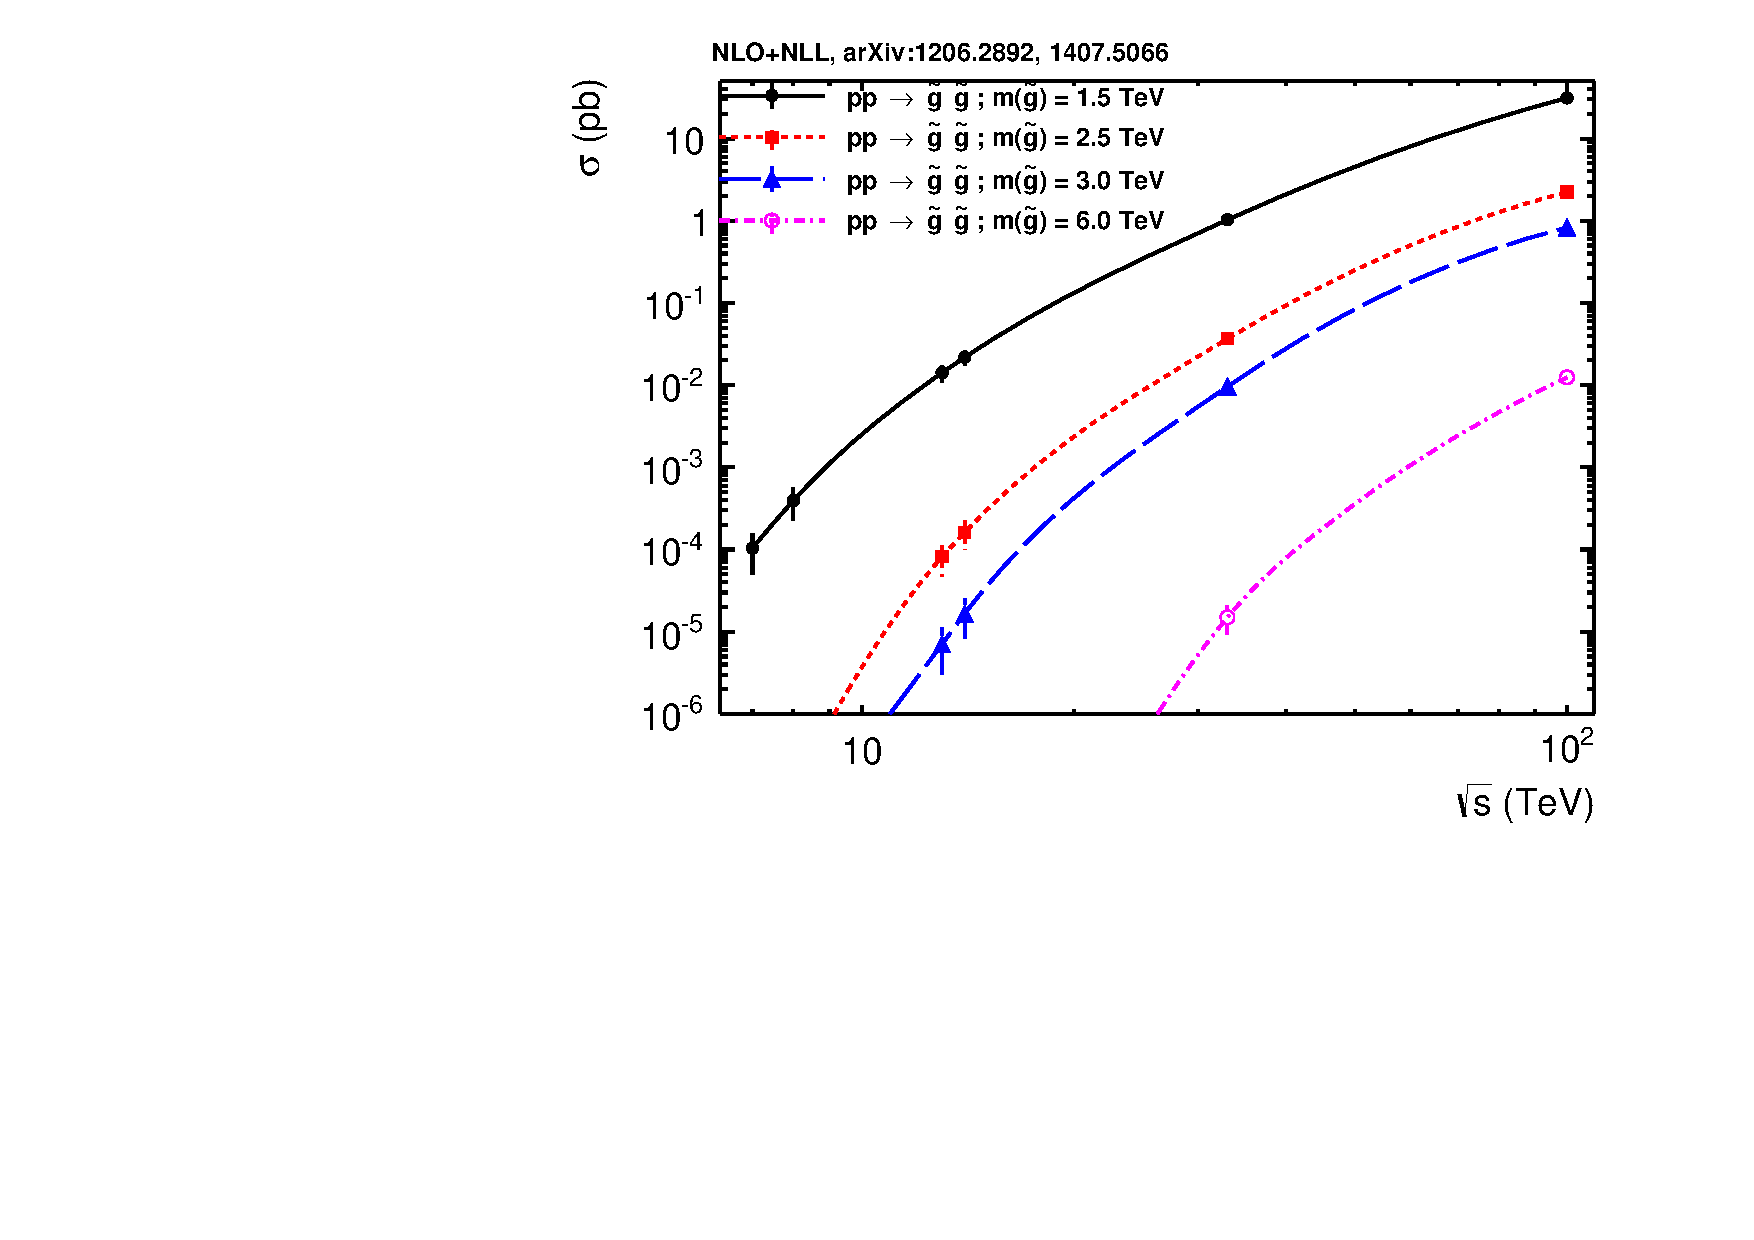
\includegraphics[width=0.495\textwidth]{figures/gluino_xsec.pdf}  
      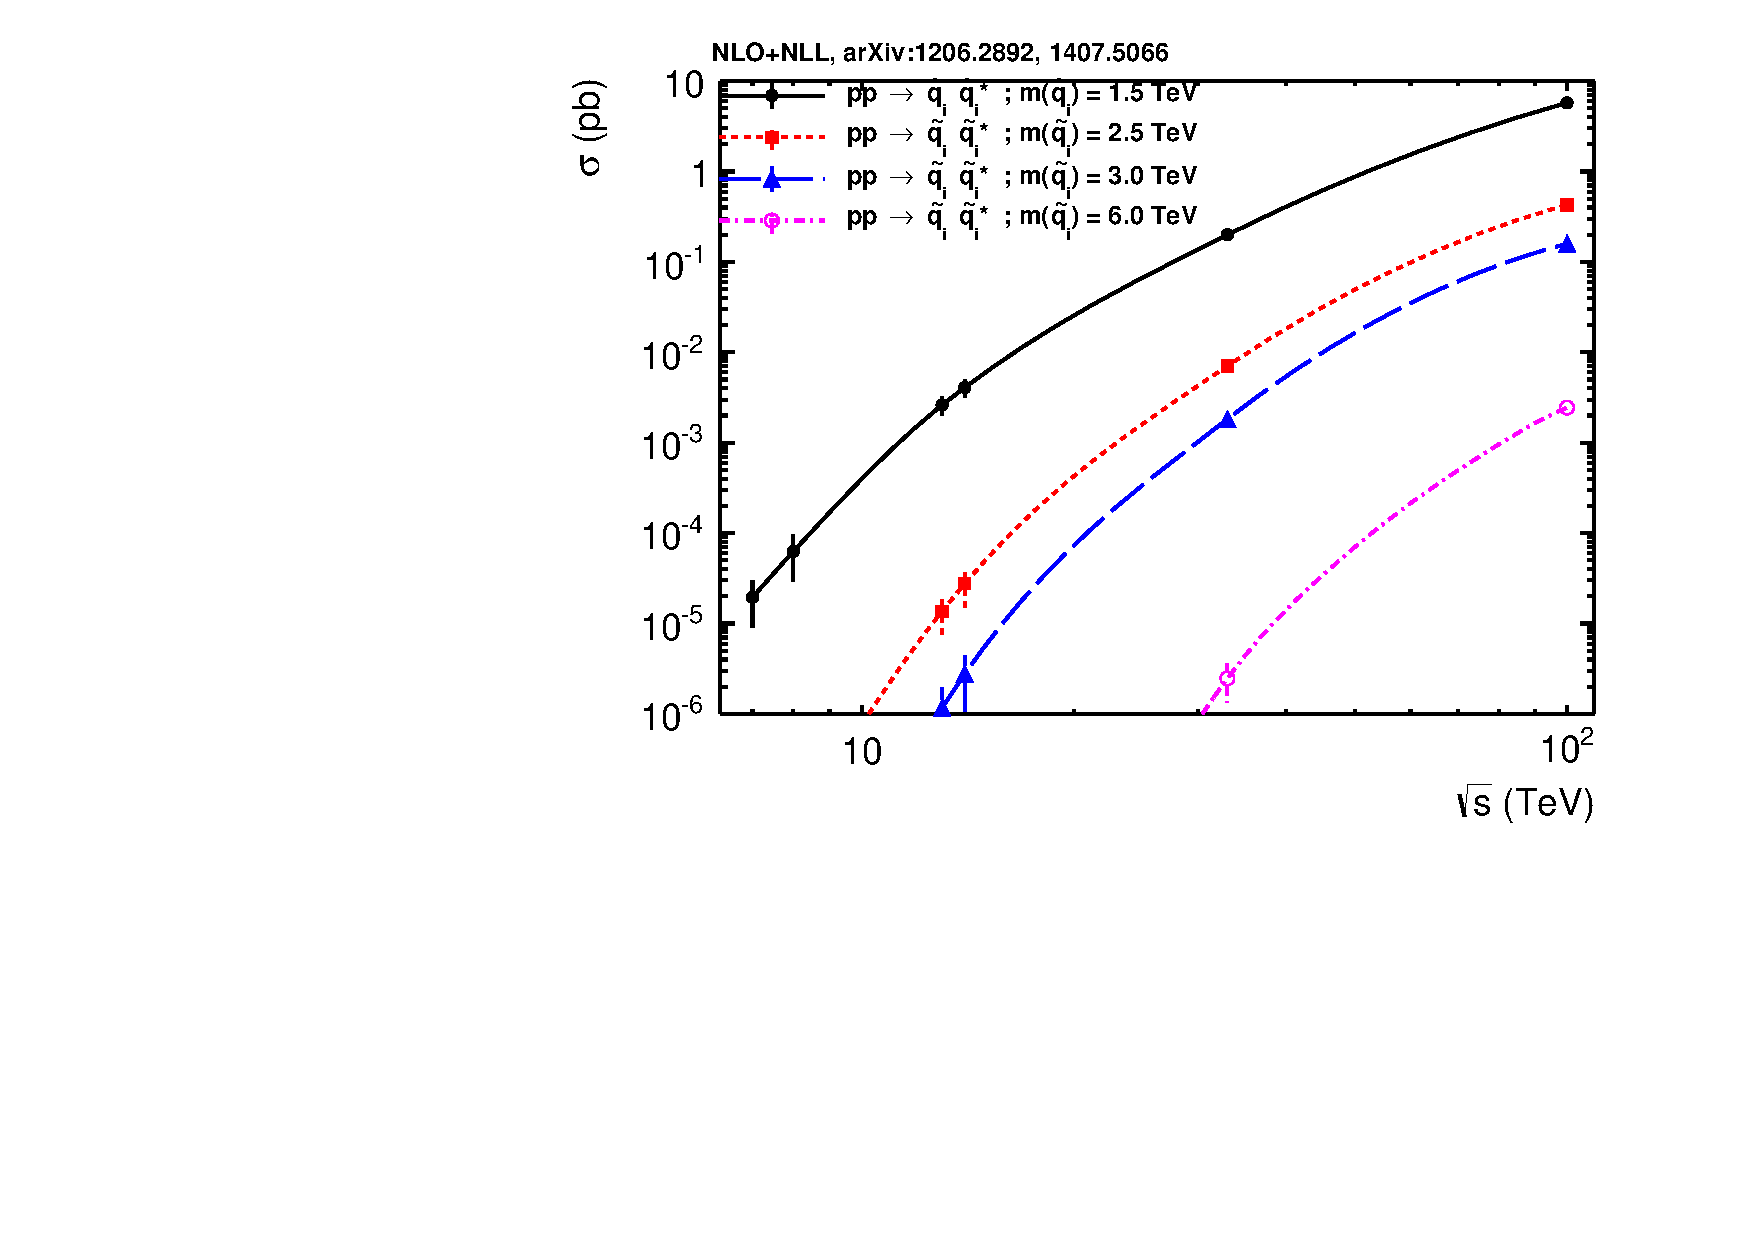
\includegraphics[width=0.495\textwidth]{figures/squark_xsec.pdf} \\
      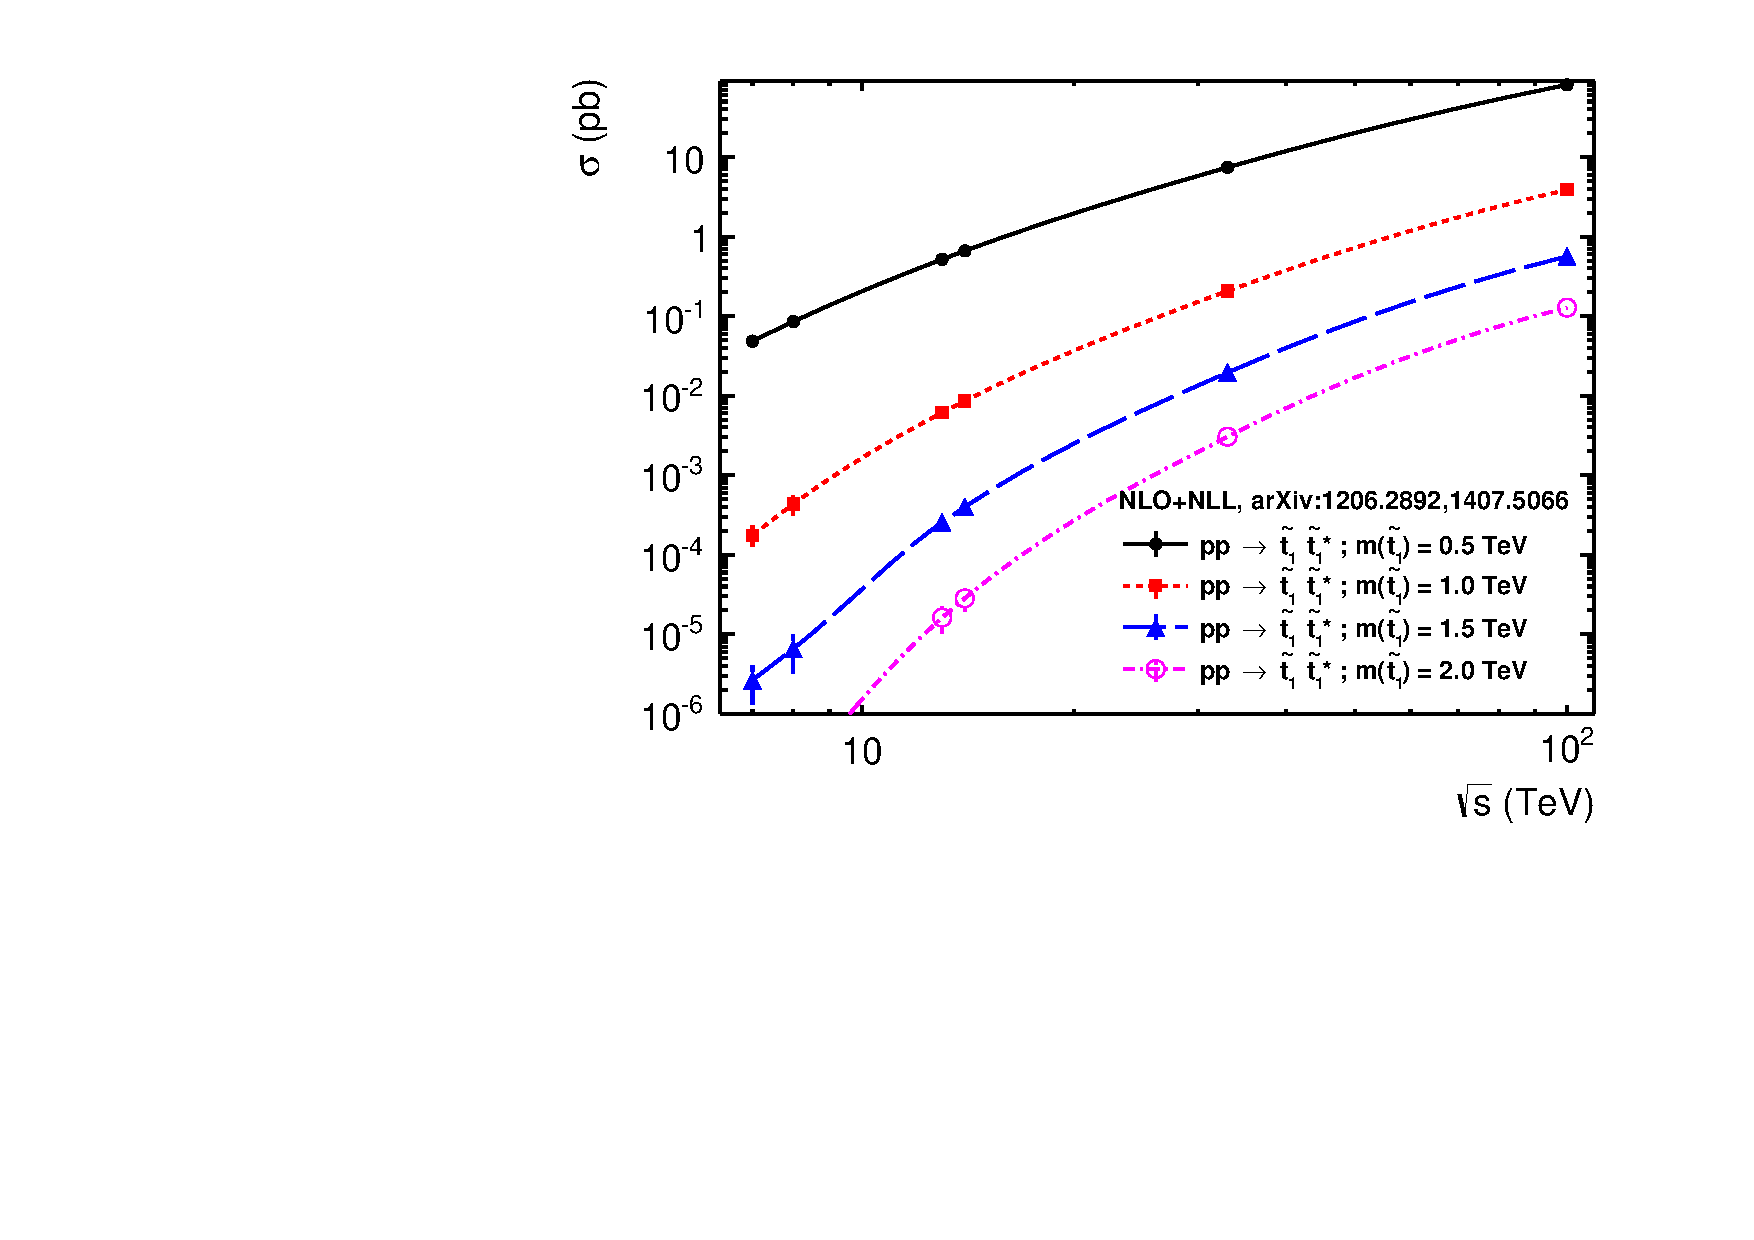
\includegraphics[width=0.495\textwidth]{figures/stop_xsec.pdf}
    \end{center}
  \end{minipage}
  \caption{SUSY production cross sections of processes $pp \rightarrow \tilde{g}\tilde{g}$ (\textit{top left}), $pp \rightarrow \tilde{q}\tilde{q}$ (\textit{top right}) and $pp \rightarrow \tilde{t}\tilde{t}$ (\textit{bottom}) displayed for different sparticle masses shown as a function of the centre-of-mass energy~\cite{Kramer:2012bx, Borschensky:2014cia}.}
  \label{fig:susy_cross_sec}
\end{figure}
\\
Most recent SUSY cross section calculations consider higher order corrections, caused for instance by quark radiation or gluon loops, typically up to next-to-leading order (NLO). Production cross sections for the processes $pp \rightarrow \tilde{g}\tilde{g}$, $pp \rightarrow \tilde{q}\tilde{q}$ and $pp \rightarrow \tilde{t}\tilde{t}$ are illustrated in Fig.~\ref{fig:susy_cross_sec} for various sparticle masses as a function of the centre-of-mass energy. For instance, for a gluino with a mass of 1.5\tev the gluino pair-production cross section is expected to be at the order of $10^{-4}$\pb at $\sqrt{s} = 7$\tev. Typically, the relative size of the different channels depends on the respective squark and gluino masses as well as the energy of the collider. While for small masses of SUSY particles or large collider energies the cross sections of gluinos are dominant, squark-pair production (and also associated squark-gluino production) are favoured in case of large SUSY masses and low collider energies. 

\subsubsection*{Decay Channels}
\label{subsubsec:susy_decay}
In addition to various different production channels, also the decay of supersymmetric particles offers a rich variety of different modes depending on the specific mass hierarchy. In Fig.~\ref{fig:susy_decay}, some example diagrams for possible decay modes of squarks and gluinos are illustrated. Here, the three-body decays of the gluinos in the upper two diagrams denote effective couplings. These occur in case squark masses are decoupled from the rest of the particle spectrum, \ie that their masses are significantly larger than that of the gluinos. \\
Gluinos decay preferrably into the LSP and a quark pair. This quark pair can for instance either be a pair of light-flavour quarks or a pair of top quarks. The latter represents the case of gluino-mediated stop production. In case of squarks, a preferred decay to the LSP and one quark is expected. While a light-flavour quark is expected from the decay of a light-flavour squark, the final state of direct production of stop quarks is made up of the LSP and a top quark.\\
In all such cases, a multijet final state accompanied by missing transverse momentum with no isolated leptons is expected as experimental signature.\footnote{In general, final state topologies including leptons can occur as well, for instance in cascade decays or semi-leptonic decays of final state top quarks. However, since the analyses presented in this thesis concentrate on all-jet final states, final states including leptons are not discussed.}  
\begin{figure}[!t]
  \centering
  % \makebox[\linewidth]{
 % \begin{minipage}[c]{1.\textwidth}
  %  \begin{center}
      \begin{tabular}{cc}
       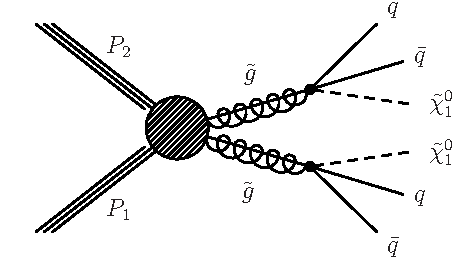
\includegraphics[width=0.49\textwidth]{figures/T1qqqq.pdf}  &
       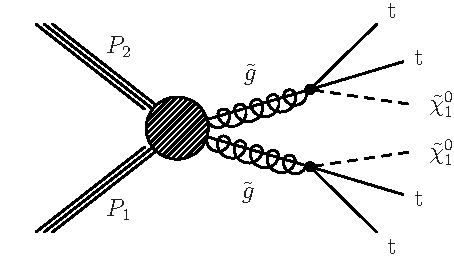
\includegraphics[width=0.49\textwidth]{figures/T1tttt_feyn.pdf} \\
       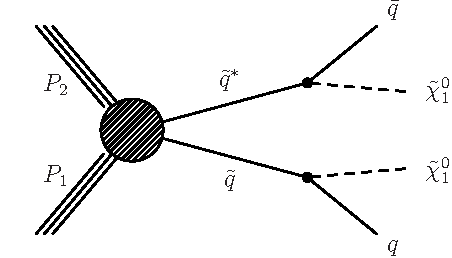
\includegraphics[width=0.49\textwidth]{figures/T2qq.pdf} &
       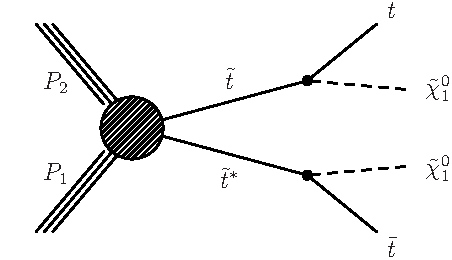
\includegraphics[width=0.49\textwidth]{figures/T2tt_v2.pdf} 
      \end{tabular}
 % \end{minipage}
  \caption{Example diagrams of different SUSY decay channels showing $\tilde{g} \rightarrow q\bar{q} \tilde{\chi}_1^0$ (\textit{top left}), $\tilde{g} \rightarrow t\bar{t}\tilde{\chi}_1^0$ (\textit{top right}), $\tilde{q} \rightarrow q\tilde{\chi}_1^0$ (\textit{bottom left}) and $\tilde{t} \rightarrow t\tilde{\chi}_1^0$ (\textit{bottom right})~\cite{bib:CMS:PhysicsResultsSUS}.}
  \label{fig:susy_decay}
\end{figure}

\subsubsection*{Background Processes in Hadronic SUSY Searches}
\label{subsubsec:susy_backgrounds}
Final states containing multiple jets accompanied by large values of missing transverse energy do not only arise from SUSY events, but are also realised for several SM processes. For any new physics search, such SM processes have to be considered as background which is a crucial task in each SUSY analysis. In case of multijet + \met searches these are typically \ZInvJets events in which large genuine \met is caused by the neutrinos. This background is denoted \textit{invisible Z background} in this thesis. Furthermore, events with intrinsic missing energy stem from \WJets and \ttbar events. 
%The top quark is the heaviest quark in the SM with a mass of $173.34 \pm 0.76$\gev~\cite{ATLAS:2014wva}. Since its lifetime is smaller than the hadronisation timescale, it decays before it forms colour-neutral hadrons. The decay takes place via the weak interaction and as denoted in Sec.~\ref{sec:sm}, the quark mixing is parametrized by the CKM-matrix. Since the corresponding matrix element $V_{\mathrm{tb}} \approx 1$, 
The top quark decays almost exclusively into a $W$ boson and a $b$ quark. Experimentally, the decay of the top-quark is characterized by the decay of the $W$ boson which can decay into a charged lepton and its corresponding neutrino or a pair of light quarks of the first two generations. Taking into account the three possible colour states for each quark pair, this gives rise to nine different $W$ decay modes and actually two thirds of top quark decays result exclusively in hadrons. However, since the targeted final state is assumed to contain a significant amount of missing energy only the semi-leptonic top quark decays relevantly contribute as background events. Thus, \WJets and \ttbar events featuring a decay containing an electron or muon that is not reconstructed, not isolated or falling out of the detector acceptance have to be considered as possible background. This source of background events is referred to as \textit{lost-lepton background}. Furthermore, also \WJets and \ttbar in which the lepton is a hadronically decaying $\tau$ lepton have to be accounted for. This background is known as \textit{hadronic-tau background}. Another source of background events is arising from QCD multijet events. Although these contain no intrinsic missing energy, severly mismeasured jets can give rise to large amounts of \met for instance because of instrumental effects or semi-leptonically decaying heavy-flavour quarks. This background process is denoted \textit{QCD background} in the following. Contributions from other SM processes are found to be negligible~\cite{springerlink:10.1007/JHEP08(2011)155, Chatrchyan:2012lia}.  

\subsubsection*{Results at $\mathbf{\sqrt{s} = 7}$\tev}
\label{subsubsec:susy_7tev_results}
As soon as first collision data have been obtained at the LHC at a centre-of-mass energy of $\sqrt{s} = 7$\tev, searches for supersymmetry were carried out based on various final states. Like for previous collider experiments, however, no hints of new physics have been found and the results were interpreted in various SUSY models by setting exclusion limits~\cite{bib:ATLAS:PhysicsResultsSUS, bib:CMS:PhysicsResultsSUS}. In Fig.~\ref{fig:CMSSM_7TeV}, interpretations of CMS searches for supersymmetry, based on various different hadronic and leptonic final states, are summarized in the context of the CMSSM. 
\begin{figure}[!tp]
  \centering 
  \begin{tabular}{cc}
    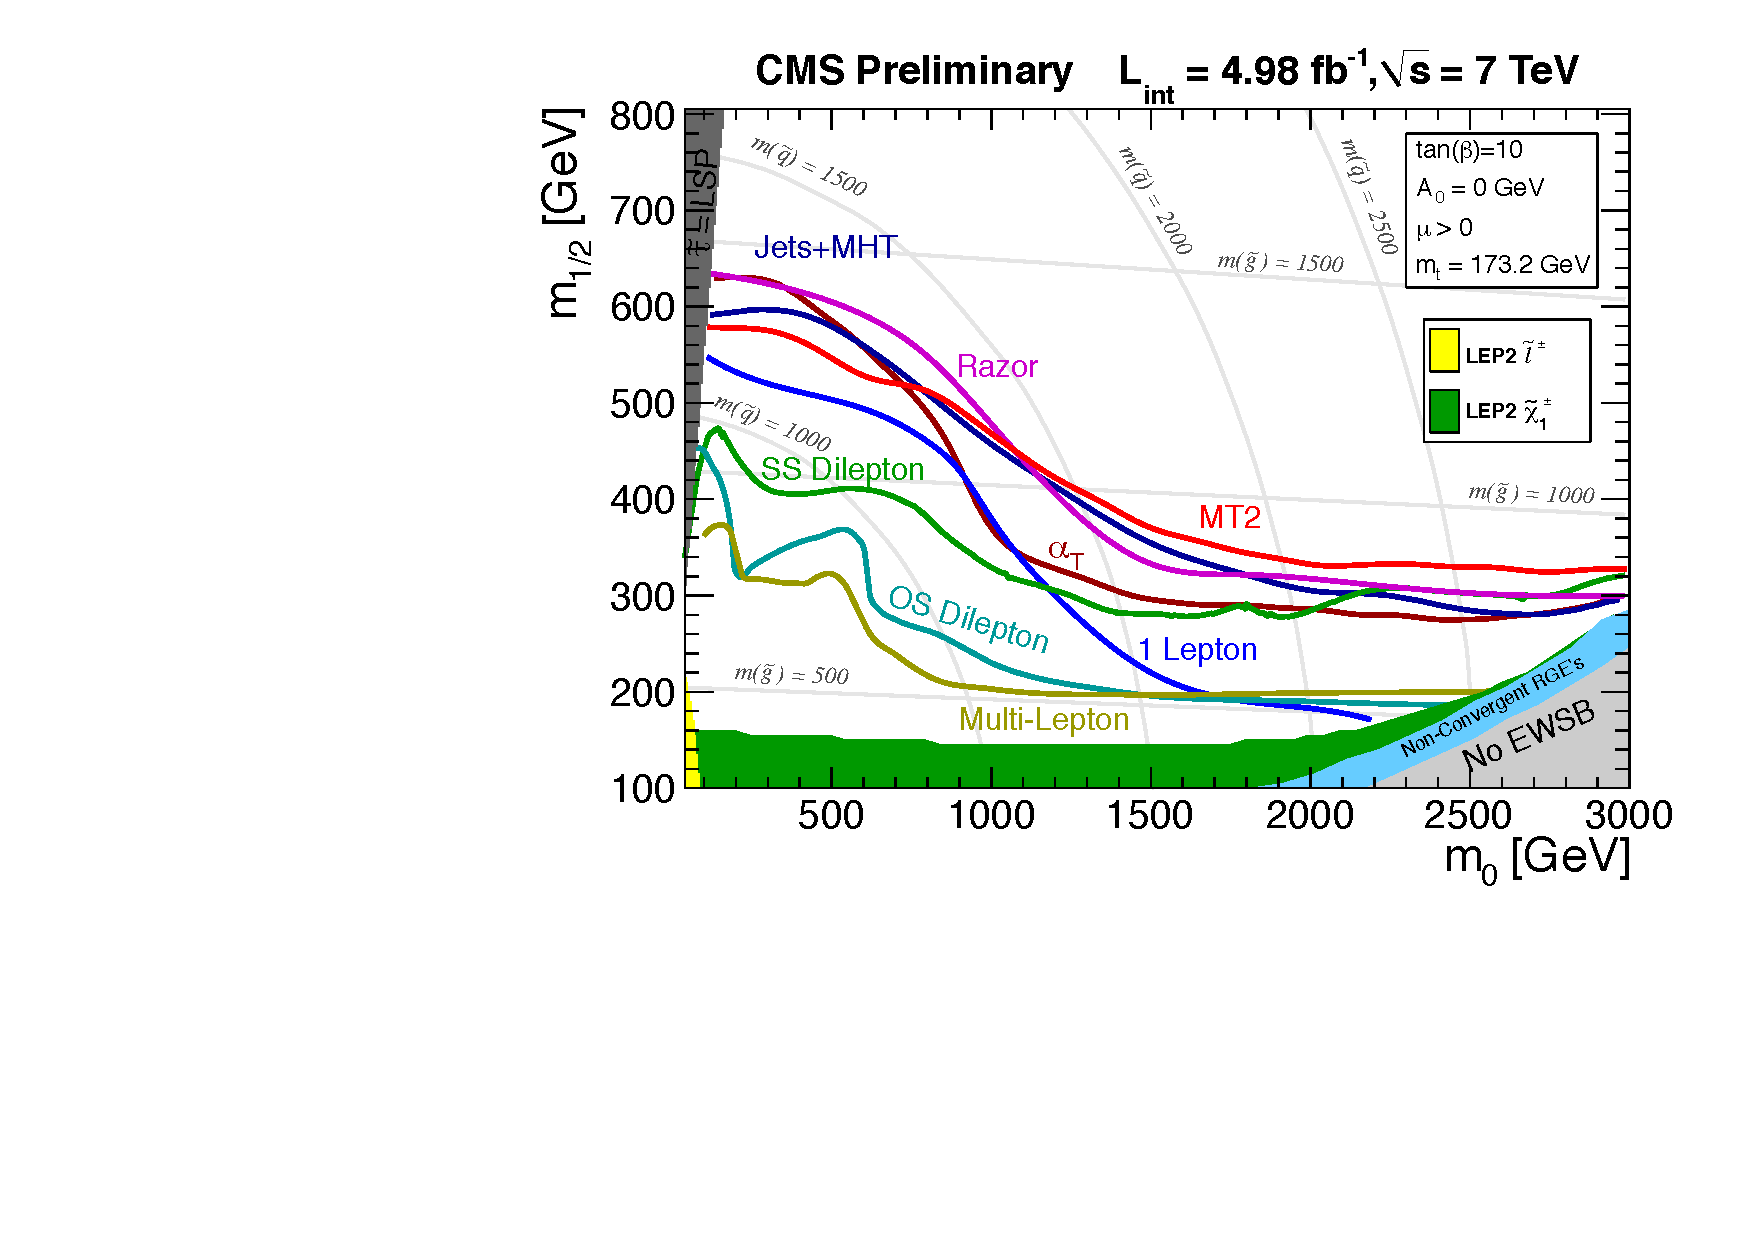
\includegraphics[width=0.7\textwidth]{figures/CMS_SUSY_2011Limits5fb_tanb10.pdf} 
  \end{tabular}
  \caption{Interpretation of searches for supersymmetry at the CMS experiment within the CMSSM. Shown are the 95\% C.L. exclusion limits in the $m_0$ and $m_{1/2}$ plane for various searches performed using different final state topologies~\cite{bib:CMS:PhysicsResultsSUS}.}
  \label{fig:CMSSM_7TeV}
\end{figure}
For comparison, also the exclusion curves from the LEP experiments~\cite{LEPLimits} are illustrated in the $m_0/m_{1/2}$-plane which have been widely exceeded already with those early searches performed at the LHC. In general, the exclusions in the CMSSM $m_0/m_{1/2}$-plane translate into constraints on the respective sparticle masses of around 1.3\tev in case of $m_{\tilde{g}} = m_{\tilde{q}}$ obtained from searches based on hadronic states as described above. However, interpreting search results only in the context of the CMSSM carries some risks. The simplified assumption of universal gaugino masses at the GUT scale does not allow all mass patterns and signatures that are in general possible within the MSSM. Consequently, the CMSSM imposes for some SUSY topologies too strong constraints. \\
Thus, results of SUSY searches are, in addition to interpretations in the CMSSM, also interpreted in the context of \textit{simplified models}~\cite{ArkaniHamed:2007fw, Alwall:2008ag, Alwall:2008va, Chatrchyan:2013sza}. Since often, many SUSY models predict a similar phenomenology, simplified models do not rely on detailed descriptions of specific model parameters, but moreover characterize the dominant features of SUSY events that are common for several SUSY and SUSY-like models. The characterization of basic properties allows a comparison of search results to any (more complex) model and provides a suitable framework for reinterpretations of results from SUSY searches. A simplified model is described by a set of particles, their masses and a certain sequence of the particle production and decay. Typical benchmark scenarios are for instance those illustrated in Fig.~\ref{fig:susy_decay} in which the only free parameters are the two sparticle masses. The branching ratios of the pair-produced initial particles into the final state particles are assumed to be 100\%. Interpretations of SUSY searches at the CMS experiment within the context of these simplified models are shown in Fig.~\ref{fig:SMS_7TeV} for $\tilde{g} \rightarrow qq\tilde{\chi}^0$ and $\tilde{q} \rightarrow q \tilde{\chi}^0$. These illustrate the 95\% confidence level upper limit on the product of the cross section and branching fraction as a function of the sparticles masses. Hence, the values of cross section times branching ratio can be compared to any theoretical prediction in order to determine whether the specific model is compatible with data. The exclusion curves shown in Fig.~\ref{fig:SMS_7TeV} indicate that, in the context of these specific simplified models, gluinos with masses up to around 1\tev and light-flavour squarks around 800\gev are excluded in case of LSP masses up to around 100\gev.
\begin{figure}[!t]
  \centering 
  \begin{tabular}{cc}
    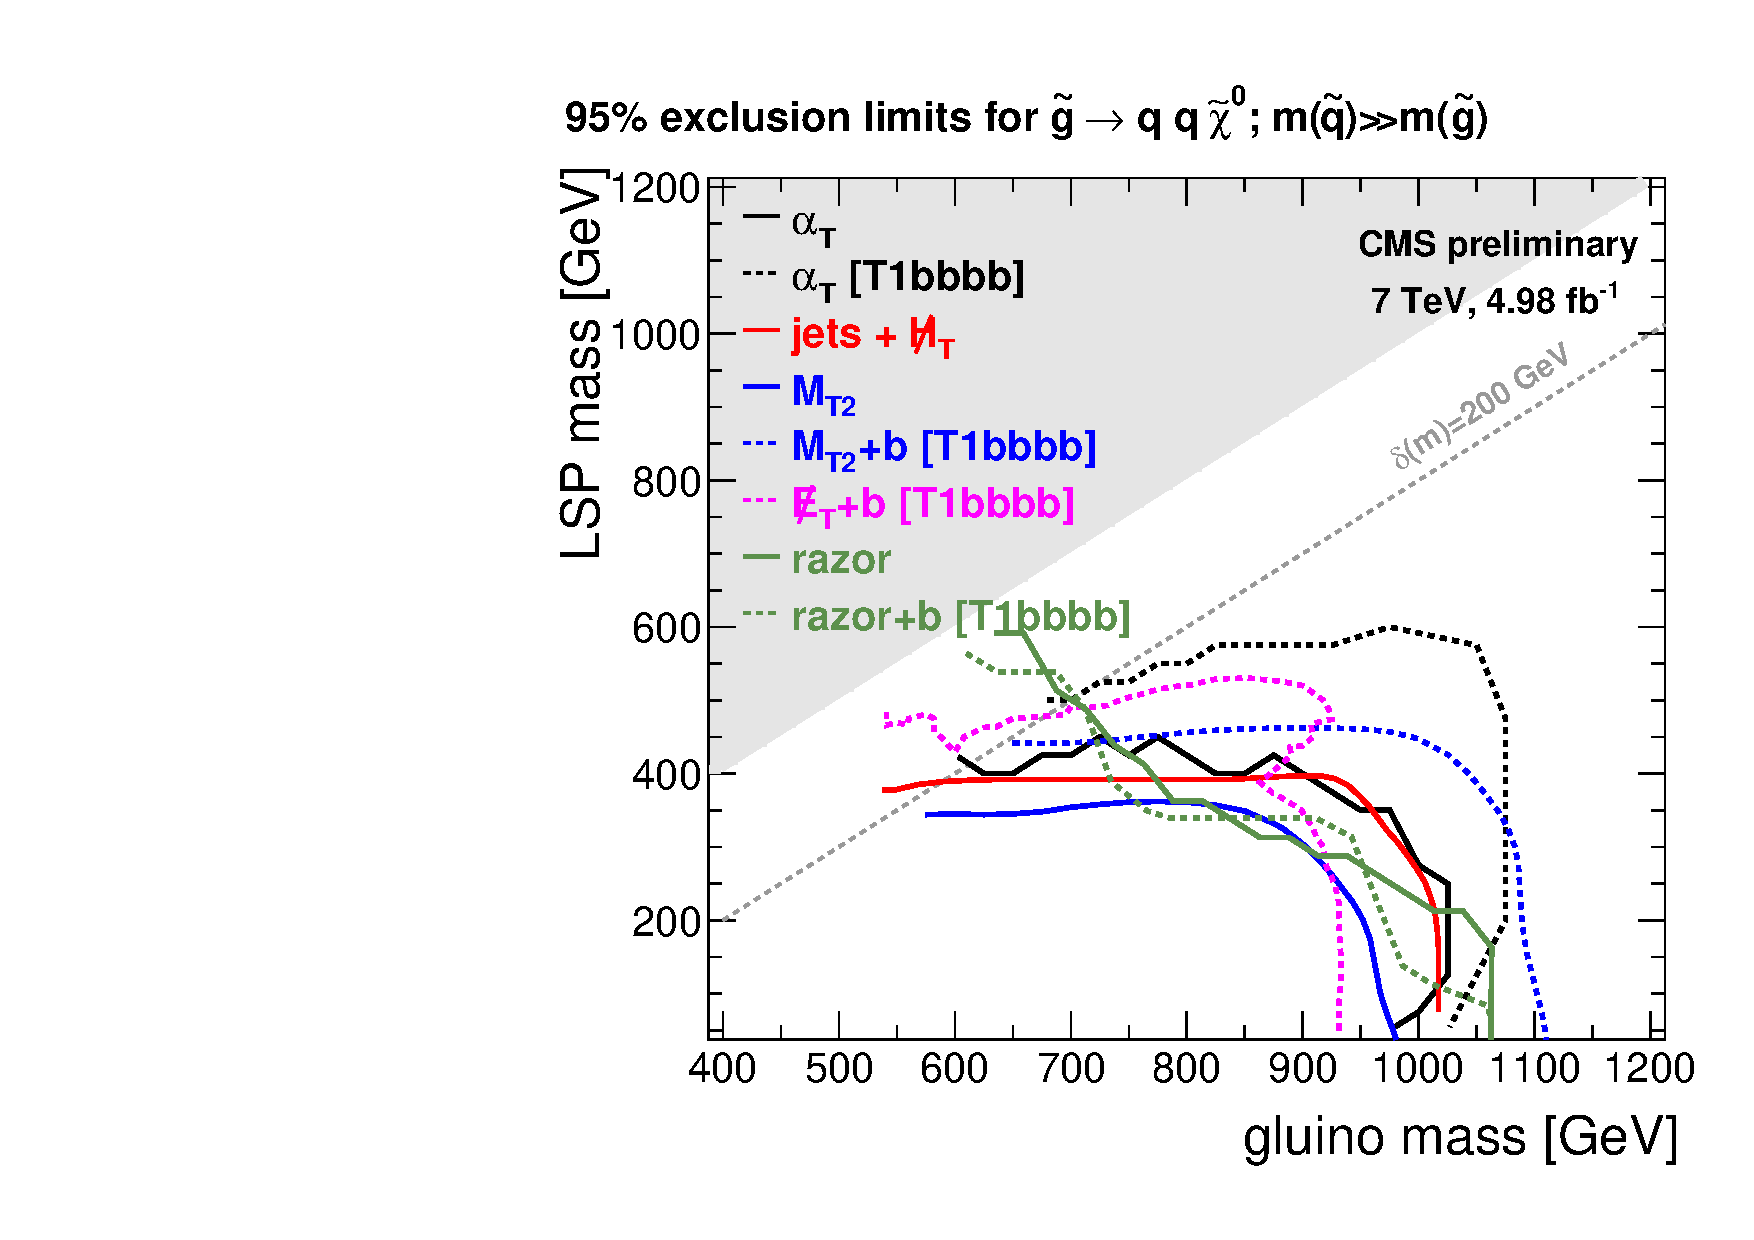
\includegraphics[width=0.49\textwidth]{figures/T1_7TeV.pdf} &
    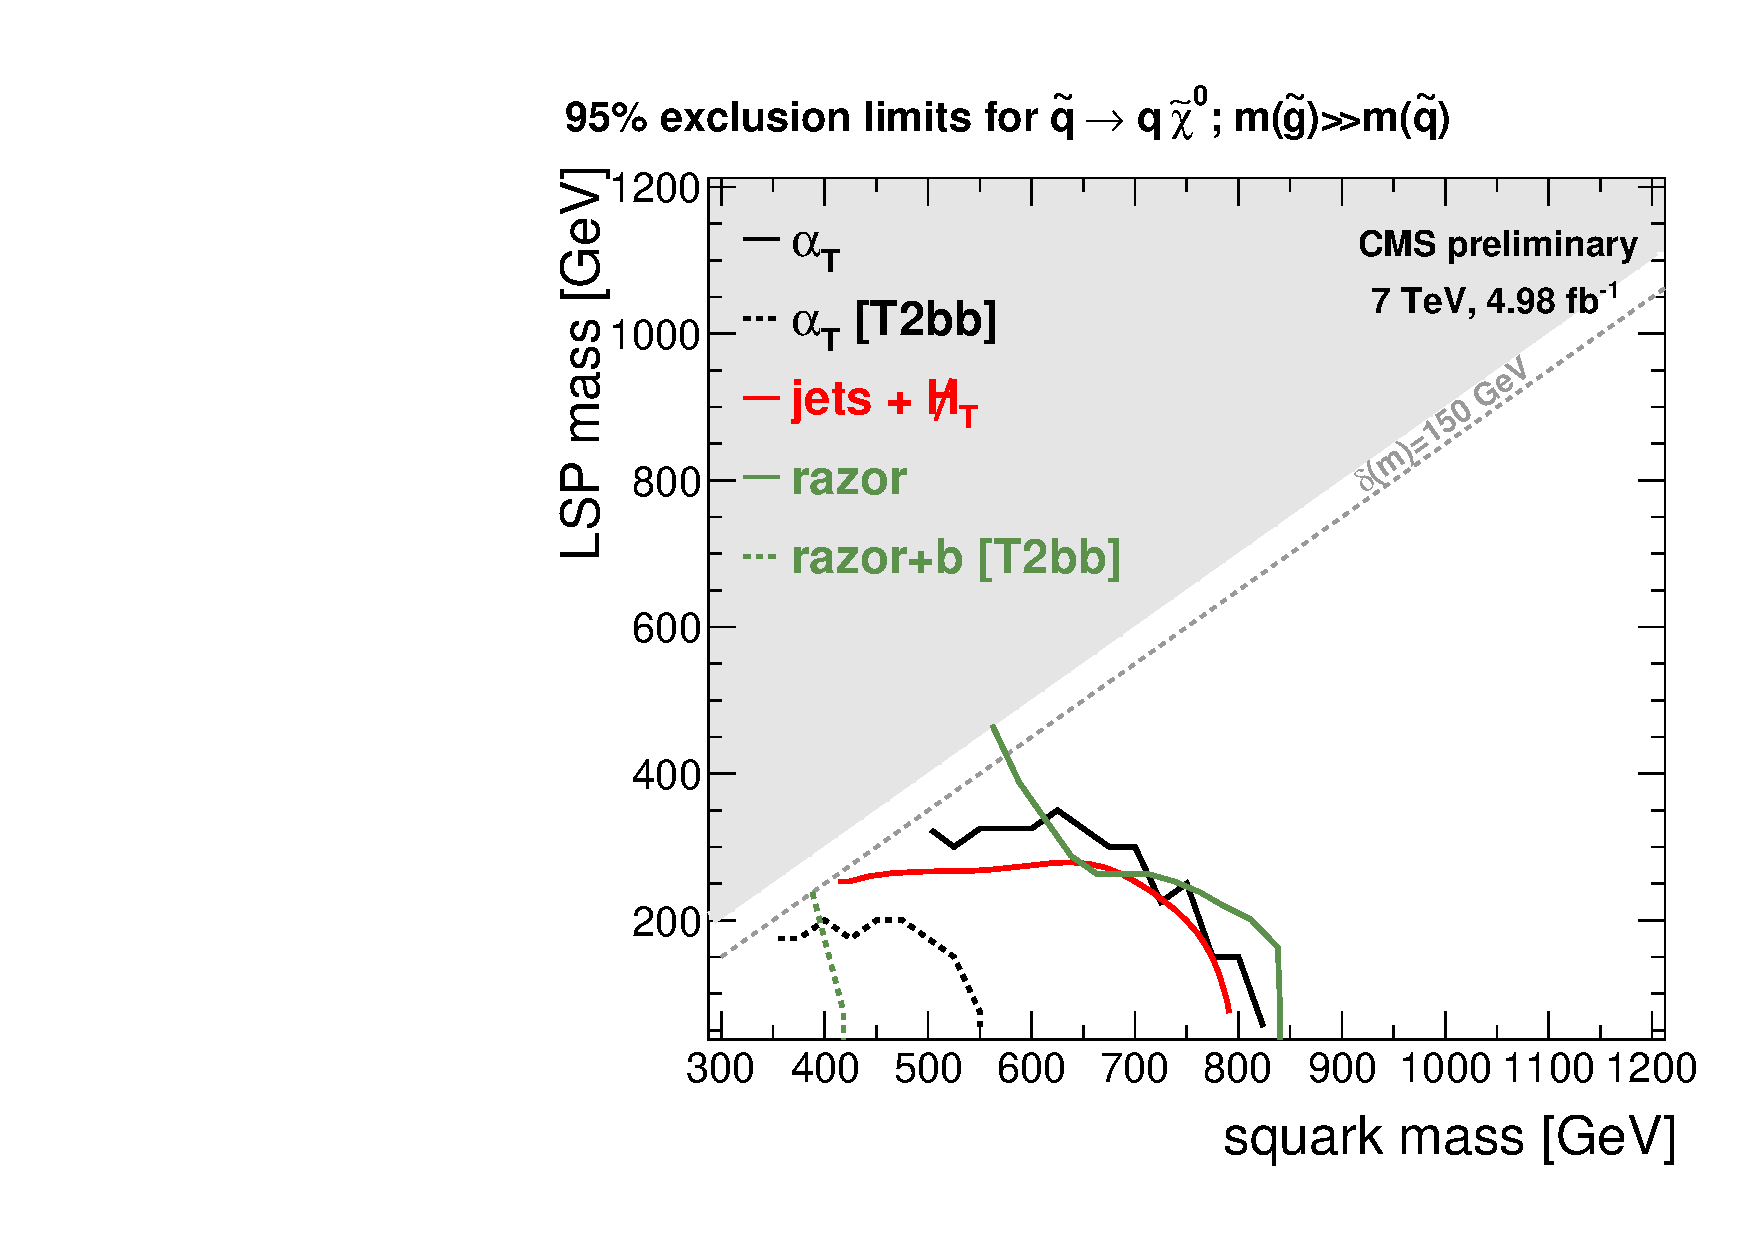
\includegraphics[width=0.49\textwidth]{figures/T2_7TeV.pdf}
  \end{tabular}
  \caption{Interpretation of searches for supersymmetry at the CMS experiment with simplified models in $\tilde{g} \rightarrow qq\tilde{\chi}^0$ (\textit{left}) and $\tilde{q} \rightarrow q \tilde{\chi}^0$ (\textit{right}) topologies. Shown are the 95\% C.L. upper limits on the produced particle and LSP masses. The grey area represents the region where the respective decay mode is forbidden~\cite{Chatrchyan:2013sza}.}
  \label{fig:SMS_7TeV}
\end{figure}
 \\
However, interpretations in simplified models typically target only well-defined isolated SUSY topologies and thus do not account for all possible decay patterns in the MSSM. Consequently, also interpretations in more general models are desirable. One such example of a more generic SUSY model is the pMSSM~\cite{Djouadi:1998di}. The pMSSM is a 19-parameter realization of the MSSM and captures most of the features of general $R$-parity conserving SUSY models and covers a wide diversity of possible SUSY topologies. The MSSM is constrained by assuming that there is no new source of $CP$-violation, that no flavour changing neutral currents occur and that the first two sfermion generations are degenerate. Interpretations of CMS SUSY searches performed at $\sqrt{s} = 7$\tev within the pMSSM are published in~\cite{CMS-PAS-SUS-12-030}. A discussion of updated results follows in Sec.~\ref{sec:susy_status}.
\\
Although the SUSY parameter space has been investigated already extensively with the LHC data obtained at $\sqrt{s} = 7$\tev and exclusion limits on sparticle masses enter the TeV range, searches for supersymmetry stay a very important field within the CMS experiment also for $\sqrt{s} = 8$\tev. As seen already in Fig.~\ref{fig:susy_cross_sec}, production cross sections are expected to largely increase for increasing centre-of-mass energies. In particular, gluino and light-flavour squark production cross sections profit a lot from the collider energy increase such that a new parameter space is accessible. Thus, in particular searches for those sparticles based on final states containing several hard jets and high values of missing transverse momentum are of major interest for analyses of the LHC $\sqrt{s} = 8$\tev data.   








\chapter{Experimental Setup} \label{chap:Detector}
In order to probe the various aspects of the well-established standard model or search for hints of new physics beyond the SM, particle physics experiments preferentially make use of powerful particle accelerators where particles of a certain type are collided in order to probe the constituents of matter and interactions between them. The analyses presented in this thesis are all performed in the context of the CMS experiment located at the Large Hadron Collider (LHC) at CERN near Geneva. \\ 
The first part of this chapter provides an introduction to the LHC. This is followed by an overview of the detector system of the CMS experiment. Afterwards the hitherto periods of collision data taking at the LHC are discussed together with an introduction to the generation of simulated events which are used in the analysis of real data events.  
\section{The Large Hadron Collider}
\label{sec:lhc}
The Large Hadron Collider~\cite{Bruning:782076, 1748-0221-3-08-S08001} is a ring-accelerator designed to provide particle collisions of hadrons. It is built in the tunnel of the former LEP~\cite{LEPdesign} collider 45 -- 170\,m below the ground and has a circumference of 26.7\,km. The LHC is a particle-particle collider and thus composed of two rings with counter-rotating beams. The operation can be performed in different modes with either proton beams or heavy ions like e.g. lead~\footnote{All studies presented in this thesis are based on proton-proton collisions. Thus the operation with heavy ions is not discussed.}. \\
In each beam, protons are grouped together in bunches and accelerated in two evacuated beam pipes using superconducting radio-frequency cavities. With a nominal bunch spacing of 25\,ns the bunch revolution frequency is 40\,MHz. Each of the 2808 individual bunches per beam contains at design conditions $1.15 \times 10^{11}$ protons. In order to bend the beams around the LHC ring superconducting dipole magnets are used with an operation temperature of 1.9\,K. They provide a magnetic field of up to 8.33\,T while additional quadrupole and sextupole magnets are utilized to squeeze and focus the beams.\\  
Before the protons are injected into the LHC they are already pre-accelerated in various smaller accelerators up to a beam energy of 450\,GeV while passing through the injector chain Linac2 -- Proton Synchrotron Booster (PSB) -- Proton Synchrotron (PS) -- Super Proton Synchrotron (SPS). An overview of the accelerator complex at CERN is given in Fig.~\ref{fig:AccComplex}.
\begin{figure}[!tp]
  \centering
  \begin{tabular}{c}
    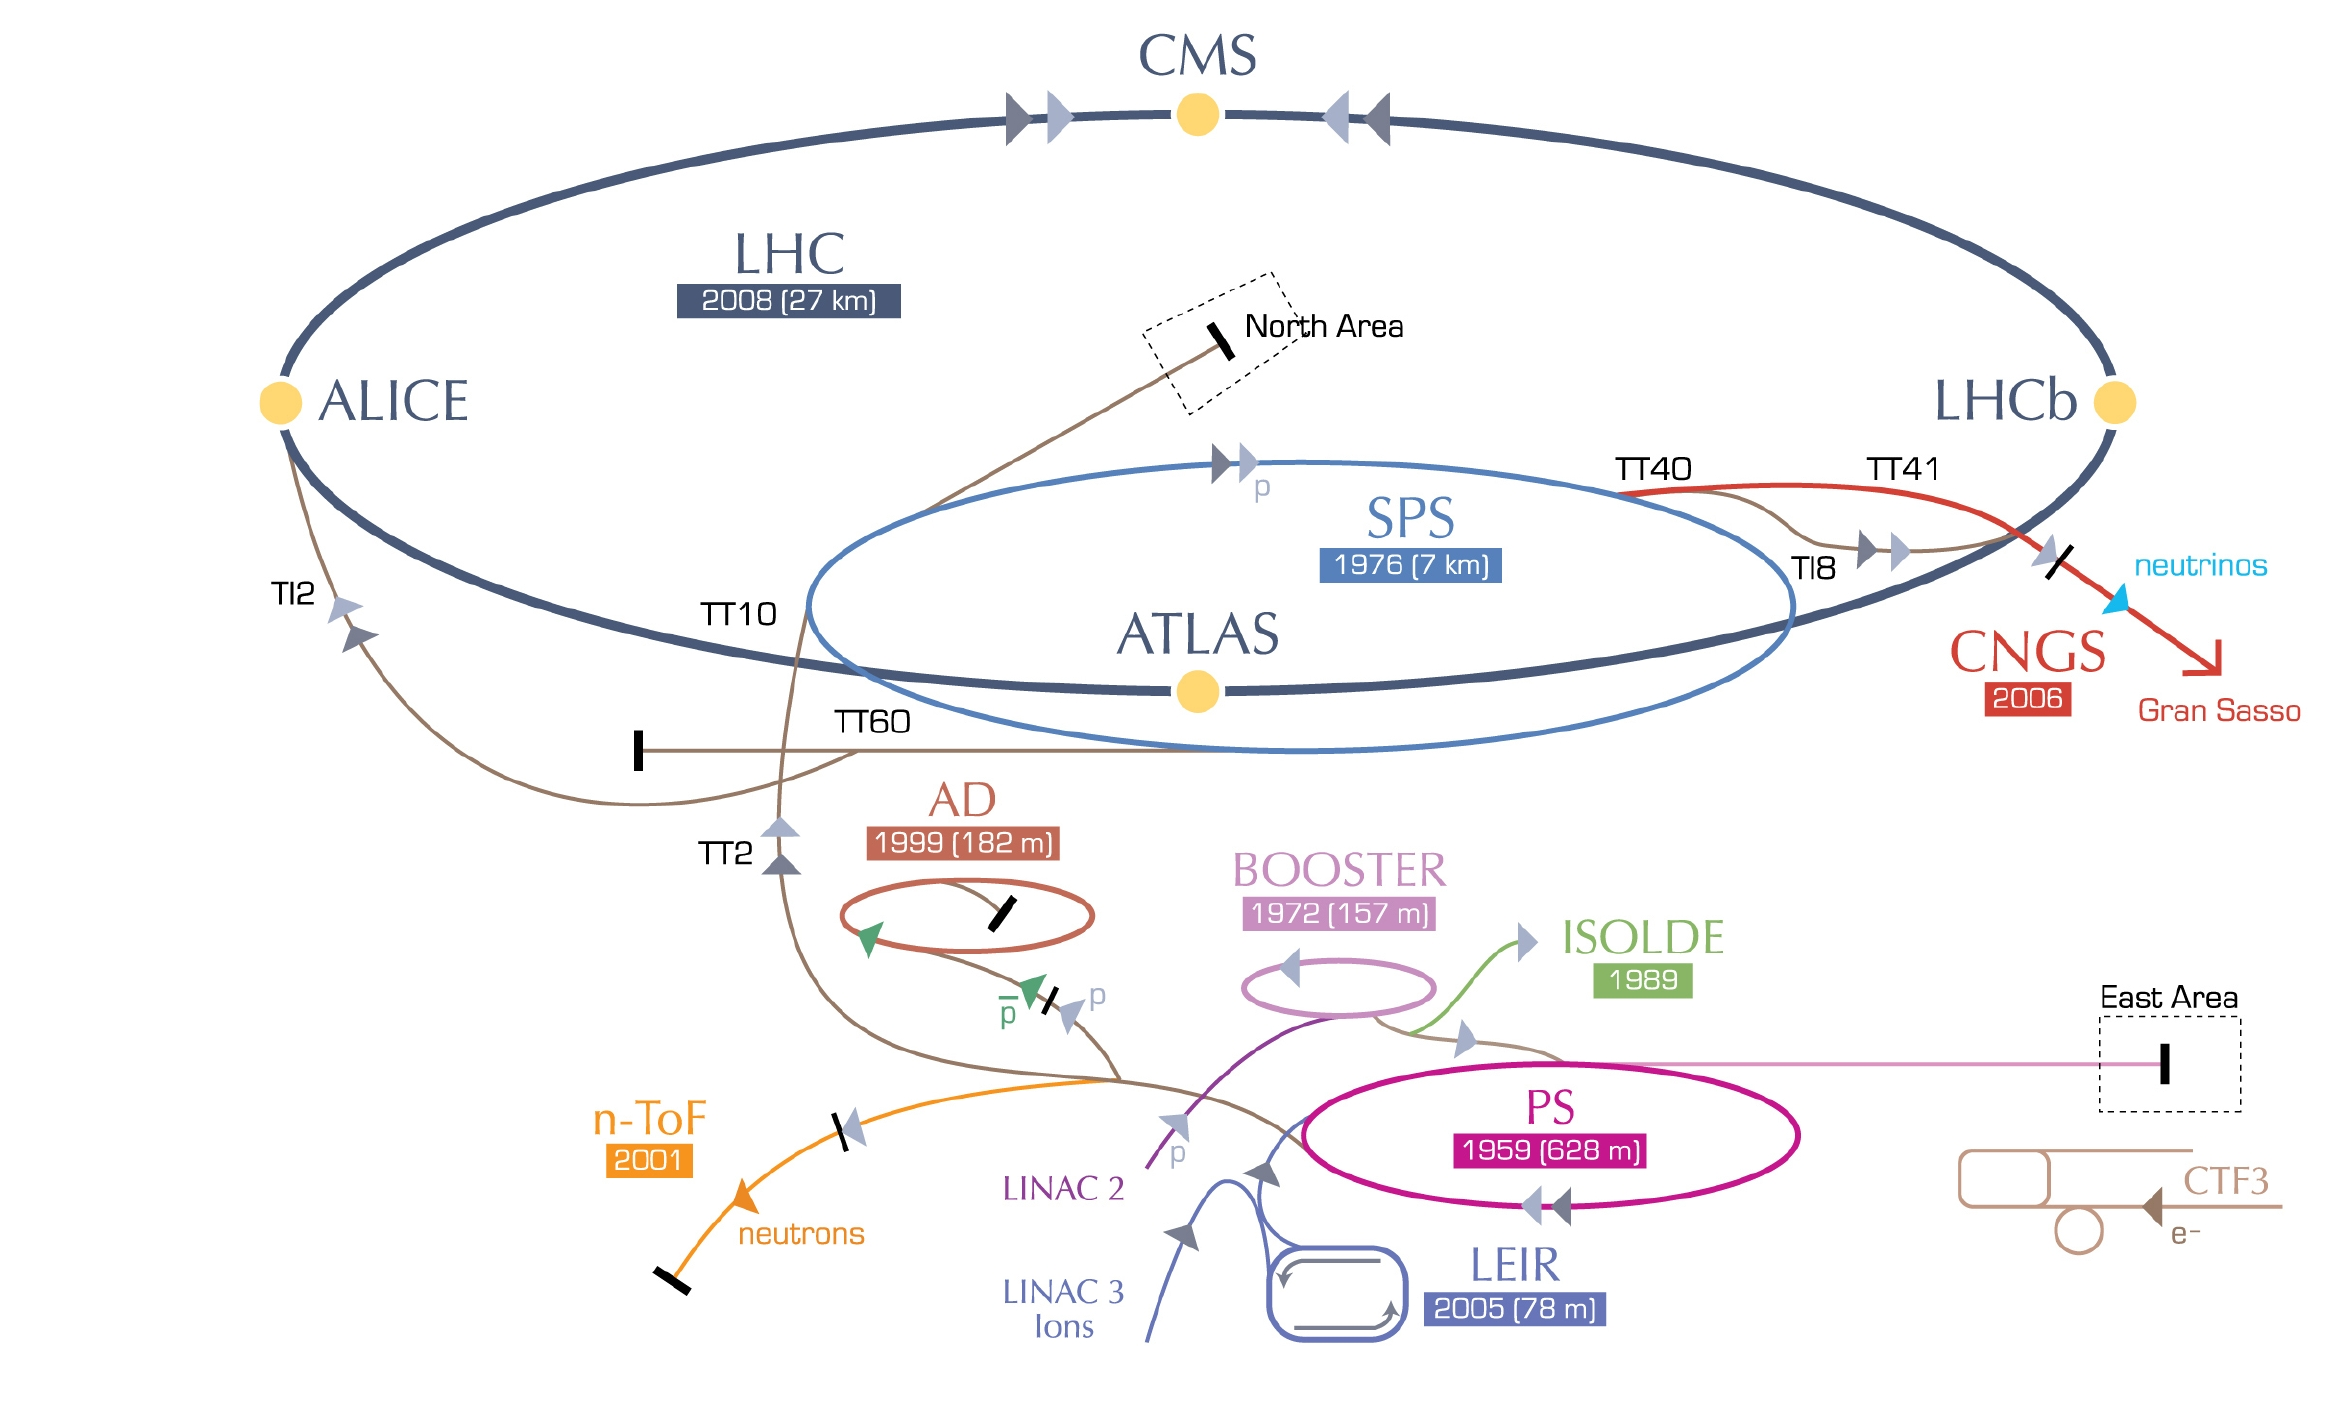
\includegraphics[width=0.8\textwidth]{figures/AcceleratorComplex.jpg}
  \end{tabular}
  \caption{Illustration of the CERN accelerator complex. Numbers below the names of individual machines indicate the year of their first operation. For ring accelerators also the circumference is given. Taken from~\cite{Christiane:1260465}.}
  \label{fig:AccComplex}
\end{figure}
\\
\\
The main goal of the LHC is to provide proton-proton collisions to the experiments with center of mass energies up to 14\,TeV in order to explore physics processes at novel energy regimes. The expected number of events $N$ for a certain type of process is given by the product of the specific cross section $\sigma$ of that process and the integral $L = \int \mathcal{L}  \, dt$ of the instantaneous luminosity $\cal L$ over time such that
\begin{equation}
  N = \sigma \cdot L . 
  \label{eq:lumi}
\end{equation}
The luminosity is a machine parameter and can be expressed for beams with Gaussian-shaped profiles as  
\begin{equation}
  \mathcal{L} = f \frac{n_{1}n_{2}}{4 \pi \sigma_{x} \sigma{y}}
  \label{eq:lumi}
\end{equation}
with the revolution frequency $f$, the number of particles $n_1$ and $n_2$ contained in the two colliding bunches and the transverse beam sizes $\sigma_{x}$ ($\sigma_{y}$) in the horizontal (vertical) directions. The nominal peak luminosity of the LHC is $10^{34} \, \mathrm{cm}^{-2} \, \mathrm{s}^{-1}$.\\
The LHC beams cross at four locations along the ring. At these interaction points the four main experiments of the LHC are located in order to measure the delivered particle collisions. The two high luminosity experiments ATLAS~\cite{det::ATLAS} and CMS~\cite{Chatrchyan:2008zzk, bib:cmsptdr1} are designed for multiple purposes like precision measurements of SM quantities, search for the standard model Higgs Boson or searches for signals indicating new physics processes. The LHCb detector~\cite{det::LHCb} however is a specialised experiment focusing on the measurement of CP violation in the interactions of hadrons containing b-quarks. The only experiment designed especially for the analysis of heavy ion collisions is the ALICE~\cite{det::ALICE} detector with the main emphasis on the physics of strongly interacting matter at extreme energy densities like for instance quark-gluon plasma.

\section{The CMS Experiment}
\label{sec:cms}
The CMS detector is one of the two experiments at the LHC designed to address a multitude of physics questions. In addition to tests of the SM at the TeV scale, studies of the nature of elektroweak symmetry breaking which might show up in the presence of a Higgs boson and searches for so far unknown particles pointing to e.g. new symmetries in nature are the primary targets of these experiments. These ambitious physics goals can only be achieved by fully exploiting the by now unprecedented collision energy and luminosity. Since the total inelastic proton-proton cross-section at a center of mass energy of 14~TeV is expected to be around 100\,mb \todo{Bild + Ref}, the experiments have to deal with an event rate of approximately $10^9$ events per second. This is resulting in high experimental challenges. The CMS detector with its typical cylindrical design of different sub-detector components around the beam line is designed to perfectly meet these particular conditions. As a typical high-energy particle experiment the CMS detector makes mainly use of tracking detectors and calorimeters to measure particles' momenta, energy depositions and flight directions in order to identify the objects emerging from the particle collisions. Table ... \todo{Performance Table} gives an overview of the performance goals of the various sub-detectors. \\  
The following sections comprise a description of the CMS detector and individual sub-detector components focusing on the detector parts most relevant for the analyses presented in this thesis. A detailed discussion of the detector design can be found in~\cite{Chatrchyan:2008zzk, bib:cmsptdr1}.

\subsection{Coordinate System and Kinematic Variables}
\label{subsec:cms_coordinates}

\subsection{Inner Tracking System}
\label{subsec:cms_tracker}

\subsection{Electromagnetic Calorimeter}
\label{subsec:cms_ecal}

\subsection{Hadronic Calorimeter}
\label{subsec:cms_hcal}

\subsection{Muon System}
\label{subsec:cms_muon}

\subsection{Trigger System}
\label{subsec:cms_trigger}

\section{Data Taking and Event Simulation}
\label{sec:data}


\chapter{Object Reconstruction and Particle Identification} \label{chap:Objects}
Particles produced in the pp collisions traverse through the detector and interact with the detector sub-components in a characteristic manner. Thus, it is possible to reconstruct the corresponding event and identify the types of particles which actually emerged from the collision. \\
The approach for the event reconstruction and identification of specific particles used in CMS is discussed in this Chapter. First, the \textit{Particle-Flow (PF) algorithm} used for a global description of the collision event is introduced. Beyond that, in particular the reconstruction of jets is discussed in Section~\ref{sec:jets_reco}. Furthermore, the identification of decays from b-hadrons and boosted top quarks is reviewed in Sections~\ref{sec:btagging} and~\ref{sec:boosted_tops}, respectively.
\section{Global Event Description with the Particle-Flow Algorithm at CMS}
\label{sec:pf_algo}
The CMS experiment introduced the Particle-Flow algorithm for the reconstruction of collision events. This algorithm is designed to identify all stable particles in an event and can be applied to data events as well as to simulated events in an identical manner. Electrons and photons, charged and neutral hadrons as well as muons are thereby distinguishable and all sub-components of the detector are used by the PF algorithm to reconstruct the particles four-momenta. The CMS detector is very well suited for this task. The silicon tracker enclosed by the uniform magnetic field enables a very efficient track reconstruction yielding only a small track fake rate down to small transverse momenta of $150$\,MeV/c. Furthermore, the strength of the magnetic field together with a high ECAL granularity allows photons to be separated from charged-particle energy deposits. A detailed introduction to the PF algorithm can be found in~\cite{CMS-PAS-PFT-09-001}. \\ 
The event reconstruction starts with the identification of fundamental objects in the sub-detectors which are charged-particle tracks, calorimeter clusters and muon tracks. Tracks emerging from charged particles are formed following an iterative tracking algorithm~\cite{Adam:934067}. Starting from an initial seed trajectory, tracks are extrapolated to further tracker layers by taking into account multiple scattering and energy loss in the material following the equations of motion of a charged particle in a constant magnetic field. Each step proceeds with a removal of unambiguously allocated hits from the previous iteration. With this approach a high tracking efficiency as well as a low fake track rate can be achieved which is a crucial requirement for a successful particle-flow event reconstruction. Furthermore, calorimeter clusters are formed in each sub-detector separately based on adjacent calorimeter cells. Neighbouring cells are combined to form clusters when their energy exceeds a pre-defined threshold. \\
A particle traversing through the detector gives typically rise to several of such elementary components so that a dedicated link algorithm is applied in order to connect these elements and form blocks while removing a potential double-counting of the same object in different detector parts. First, charged-tracks are associated to calorimeter clusters, if the extrapolated trajectory matches the cluster within the cluster boundaries. This is done considering effects like gaps and cracks between detector components, uncertainty on the shower position or multiple-scattering. Photons from Bremsstrahlung are considered by extrapolating also tangents of the tracks to the respective energy clusters. In a similar manner ECAL and HCAL clusters can be connected to each other as well by linking clusters in the more granular calorimeter to clusters in the less granular one. At last global muons can be defined by associating charged-tracks from the tracker with muon tracks reconstructed in the muon system. \\
After the identification of such blocks of elements the PF algorithm proceeds to finally create a list of all particles contained in the event applying dedicated quality criteria interpreting the blocks in terms of particles. The identification of muons and a removal of their tracks from the blocks is followed by an assignment of electrons and associated Bremsstrahlung from tracks and linked ECAL clusters. After these have been removed from the blocks as well, remaining good quality tracks are considered to be charged hadrons. Their momenta are determined from combining the track momentum and the respective energy in the calorimeter cluster. If the cluster energy largely exceeds the measured momentum from the track beyond the detector resolution, it constitutes a photon and if the excess is larger than the total ECAL energy also a neutral hadron. Finally, remaining ECAL and HCAL clusters not linked to any track give rise to photons and neutral hadrons. \\
The complete set of particles can then be used to derive further objects and quantities like e.g. jets as discussed in Section~\ref{sec:jets_reco}, missing transverse energy $E_{T}^{\mathrm{miss}}$ which is the magnitude of the vector momentum imbalance perpendicular to the beam direction, decay products of tau leptons or decays of b-hadrons as discussed in Section~\ref{sec:btagging}. 

\section{Reconstruction of Jets}
\label{sec:jets_reco}

\subsection{Jet Algorithms}
\label{subsec:jets_algos}

\subsection{Jet Types at CMS}
\label{subsec:jets_types}

\subsection{Jet Energy Calibration}
\label{subsec:jets_calib}

\section{Identification of B-Hadron Decays}
\label{sec:btagging}

\section{Identification of Boosted Top Quark Decays}
\label{sec:boosted_tops}

\subsection{The CMS Top Tagger}
\label{sec:boosted_tops_cms_tagger}

\subsection{The HEP Top Tagger}
\label{sec:boosted_tops_hep_top_tagger}

%\subsection{Subjet B-Tagging}
%\label{sec:boosted_tops_subjet_b}

%\subsection{N-subjettiness}
%\label{sec:boosted_tops_n_subjettiness}


\chapter{Measurement of the Jet Transverse-Momentum Resolution} \label{chap:Resolution}
Many measurements of standard model properties or searches for new physics beyond the standard model performed within the CMS experiment rely on events with jets in the final state. Hence, a good understanding of jet properties is of major importance and a crucial ingredient for such kind of analyses. One of such properties is the jet transverse-momentum resolution, as introduced in Sec.~\ref{subsec:jets_response}. \\
Many new physics searches are carried out based on final states containing missing transverse momentum and several jets. Here, QCD multijet events can fake the signature of possible new physics events and constitute a background process, since a mismeasurement of the jet momenta due to the limited detector resolution or the decay of heavy flavour quarks leads to a momentum imbalance in the event and consequently to measurable missing energy. The knowledge of the jet resolution is thus a keypoint in the prediction of such background contributions, as discussed later in Chap.~\ref{chap:RA2}. \\
In this chapter, an analysis is presented in which the jet-\pt resolution in data and in simulated events is derived. The method is based on momentum conservation in the transverse plane of dijet events and offers the possibility to cover a large phase space in \pt and $\eta$. A similar approach was already used in previous studies at $\sqrt{s}=7$\tev~\cite{1748-0221-6-11-P11002, thesis:Schroeder} while a complementary approach utilizes $\gamma +\rm{jet}$ events~\cite{CMS-AN-2010-141, CMS-AN-2011-004, CMS-AN-2013-179}. The measurement shown here is based on collision data corresponding to an integrated luminosity of $19.7$~\fbinv recorded at $\sqrt{s}=8$\tev in 2012. Parts of this chapter are taken from~\cite{bib:AN2013-416}, having been written by the author.   
\section{Components of the Jet Response}
\label{sec:jer_response}
\begin{figure}[!tp]
  \centering
  \begin{tabular}{c}
                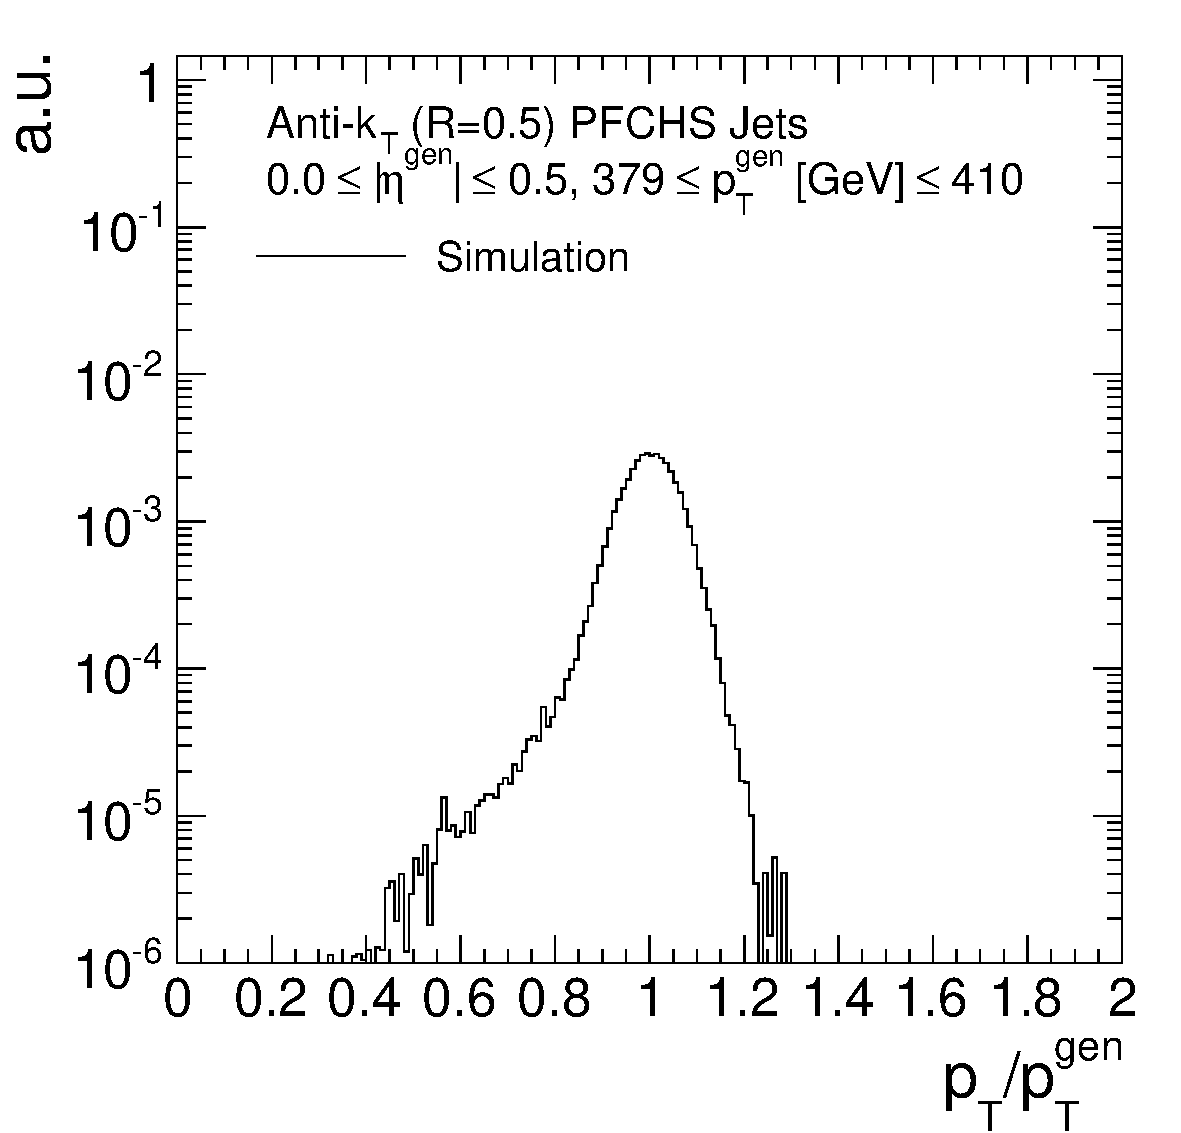
\includegraphics[width=0.49\textwidth]{figures/TruthResponse_example_test.pdf}
  \end{tabular}
  \caption{Jet response distribution for one example $|\eta^\mathrm{gen}|$ and $\pt^\mathrm{gen}$ interval derived from simulation.}
  \label{fig:response}
\end{figure}
As introduced in Sec.~\ref{subsec:jets_response}, the relation of the transverse momentum of a jet at detector level to the momentum of the corresponding particle-level jet is expressed by the jet response. In simulated events, the transverse momentum of the particle-level jet is known and corresponds to the \pt of the generated jet, which is clustered from all stable particles after hadronisation and decay, including neutrinos. Thus, the \textit{MC-truth response} can be determined as
\begin{equation}
\mathcal{R} = \frac{\pt}{\pt^{\mathrm{gen}}} \; .
\end{equation}
 In Fig.~\ref{fig:response}, an example for a jet response distribution derived from simulation is shown. It is obtained from a QCD multijet sample generated with $\textsc{Pythia6}$ tune Z2~\cite{Chatrchyan:2011id} using the CTEQ6L1 PDF set~\cite{Pumplin:2002vw} and processed with the full detector simulation. For the calculation of the truth response, the two generated jets in the event with highest transverse momentum are selected. The event is rejected, if one of these two generator jets does not have a corresponding reconstructed jet within a distance of $\Delta R < 0.25$. Otherwise, the response is calculated in intervals of $\pt^\mathrm{gen}$ and $|\eta^\mathrm{gen}|$. This is done since a dependence on the momentum and the respective detector region is expected, as discussed in Sec.~\ref{subsec:jets_response}. The calculation of the jet response is performed after applying the jet energy corrections discussed in Sec.~\ref{subsec:jets_calib} to the detector-level jet momenta, so that the mean of the response distribution is located at one. \\
Apparently, the jet response distribution consists of two components: the Gaussian-shaped core around the mean referred to as jet resolution and non-Gaussian components referred to as tails. \\
The core of the response is mainly caused by the intrinsic resolution of the various sub-detector components and the precision of the PF algorithm. Since the jet momenta obtained from the PF constituents are based on tracking- as well as calorimeter-based measurements, the jet resolution is closely connected to the evolution of the tracking and calorimeter resolution with \pt. In the tracking system, the intrinsic resolution is mainly caused by the uncertainty on the track curvature. This is limited by multiple scattering at low \pt and by the finite hit-position resolution at high \pt. In total, the track-\pt resolution degrades for increasing transverse momentum. However, the evolution of the resolution in the calorimeters behaves the other way round and improves with increasing momentum. At low momenta, the calorimeter resolution is mainly dominated by electronic noise and pileup while at medium momenta the resolution is driven by fluctuations of the shower development. At high energies, however, the resolution is eventually limited by calorimeter miscalibration and non-uniformities. Furthermore, the response also depends on the jet flavour. Typically, quark jets consist of less and harder particles than gluon jets and thus have a different detector response due to the non-linearity of the calorimeters.  \\
The response tails are caused by severe jet-momentum mismeasurements. These can for instance be due to detector effects. Shower leakage can occur, if not the whole shower is deposited in the calorimeters. Due to the limited length of the calorimeters, some particles might even cross the whole apparatus (\textit{punch-through}). Also malfunctioning detector components can lead to high or low reponse tails by creating artifical signals. Beyond that, also physics processes lead to response tails. For instance, the lower response tails get populated by semi-leptonic decays of heavy-flavour quarks. These contain neutrinos that carry a certain amount of the momentum and leave the detector unnoticed resulting in an overall reduced response. 

\section{Basic Concept of the Dijet Asymmetry Method}
\label{sec:jer_method}
As introduced in Sec.~\ref{subsec:jets_response} and~\ref{sec:jer_response}, the jet transverse momentum resolution corresponds to the width of the Gaussian-shaped core part of the jet response. In simulated events, the particle-level jet momenta are given by the generator-level jet momenta. In data events, however, no such equivalent is present so that the jet resolution is not accessible directly. \\
One possibility to measure the resolution of the jet transverse momenta in data as well as in simulated events is to utilize the dijet asymmetry $\mathrm{A}$. For events with at least two jets it is defined as
\begin{equation}
\label{eq:asymmdef}
  \mathrm{A} = \frac{p_\mathrm{T,1} - p_\mathrm{T,2}}{p_\mathrm{T,1} + p_\mathrm{T,2}} \, .
 \end{equation}
 In this equation $p_\mathrm{T,1}$ and $p_\mathrm{T,2}$ correspond to the randomly ordered transverse momenta of the two leading jets. \\
 Neglecting tails, the asymmetry is approximately normally distributed, with mean $= 0$, and the standard deviation is given as
 \begin{equation}
 \label{eq:asymm_first}
  {\sigma_{\mathrm{A}}} = \left\lvert \frac{\partial \mathrm{A}}{\partial p_\mathrm{T,1}} \right\rvert \cdot \sigma(p_\mathrm{T,1}) \oplus  \left\lvert \frac{\partial \mathrm{A}}{\partial p_\mathrm{T,2}} \right\rvert \cdot \sigma(p_\mathrm{T,2}) \; .
 \end{equation}
 In an ideal dijet topology, the two jets are exactly balanced at particle level. If they belong in addition to the same $\eta$ region, then $\langle p_\mathrm{T,1} \rangle = \langle p_\mathrm{T,2} \rangle = \langle \pt \rangle$ and $\sigma (p_\mathrm{T,1}) = \sigma (p_\mathrm{T,2}) = \sigma (\pt)$. This allows the simplification of Eq.~\ref{eq:asymm_first} and provides the following important relation between the width of the asymmetry $\sigma_\mathrm{A}$ and the jet-\pt resolution $\sigma (\pt)$
 \begin{equation}
 \label{eq:asymm}
  \frac{\sigma (p_\mathrm{T})}{\langle p_\mathrm{T} \rangle} = \sqrt{2} \cdot \sigma_\mathrm{A} \; .
 \end{equation}
This relationship was already used at the Tevatron experiments~\cite{oai:arXiv.org:hep-ex/0012046, JetsD0}, the ATLAS experiment~\cite{Aad:2012ag} or in previous CMS analyses~\cite{1748-0221-6-11-P11002, thesis:Schroeder} to measure the jet resolution from dijet events. 

\section{Application to Realistic Collision Events}
\label{sec:jer_application}
The measurement of the jet transverse momentum resolution in collision events is based on Eq.~\ref{eq:asymm}. As discussed in Sec.~\ref{subsec:jets_response}, the resolution is a function of \pt and $\eta$. In order to account for this dependence, the asymmetry has to be recorded in intervals of pseudorapidity and a measure for the transverse momentum scale of the event, as \eg the \pt of the leading jet, as well. However, the jet-\pt spectrum is affected by migration effects such that momentum measures based on single jets are not preferable. Due to the limited jet resolution, a particular interval of reconstructed jet momenta is populated not only by jets whose particle-level jet momentum belongs to that bin. In case of a steeply falling spectrum, as it is the case for jet momenta, more jets with low $\pt^\mathrm{gen}$ migrate into a specific interval than jets with high $\pt^\mathrm{gen}$. Consequently, the measured response is systematically higher and the measured relative response is biased towards the object with worse resolution. In order to reduce this resolution bias in the analysis, the measurement is performed in intervals of the average momentum of the two leading jets in the event
\begin{equation}
\ptave = \frac{1}{2}(p_\mathrm{T.1} + p_\mathrm{T,2}) \; .
\end{equation}
Beyond that, the ideal dijet topology with exactly two jets that are perfectly balanced, is interferred with additional effects in realistic collision events. Very often, further jet activity is occuring as momentum of the hard scattering process is transferred to soft particles or jets arising from initial or final state radiation leading to momentum imbalance in the dijet system. This additional jet activity can be described by the variable $\alpha$ which is defined as the ratio of the transverse momentum of the third jet to the average momentum according to
 \begin{equation}
\label{eq:alpha}
\alpha = \frac{p_\mathrm{T,3}}{\pt^\mathrm{ave}} \, .
\end{equation}
The presence of jets beyond the third is neglected in the parametrization of the additional activity in the event, as these have consecutively declining momentum due to the strongly decreasing jet production cross section versus jet-\pt~\cite{CMS-PAS-QCD-11-004}. The presence of additional jets and the thereby introduced imbalance leads to a broadening of the observed asymmetry distribution. This effect is also illustrated later in Sec.~\ref{subsec:jer_sel_cuts}. In order to determine the intrinsic resolution from such events, the measured resolution has to be corrected for this effect. \\
A further source of momentum differences between the particle-level and the detector-level jet leading to an overall momentum imbalance in an event is arising from out-of-cone showering effects. Typically, some particles might be too soft to be included in the clustered jet. Furthermore, additional contributions from the underlying event might be wrongly asscociated to a jet. In general, such effects have to be considered in the resolution measurement as well. \\
The actual procedure how to determine and apply the required corrections is discussed in Sec.~\ref{sec:jer_corrections}.

\section{Samples and Event Selection}
\label{sec:jer_selection}
%In this section the data samples used for the analysis are specified (Section~\ref{subsec:jer_samples_and_trigger}). Furthermore, selection criteria applied on data and simulated events in order to select events with a dijet-like topology are discussed (Section~\ref{subsec:jer_sel_cuts}). 

\subsection{Datasets and Triggers}
\label{subsec:jer_samples_and_trigger}
\begin{table}[!tp]
\centering
\caption{Trigger paths with \ptave thresholds at which the trigger efficiency reaches the $99\%$ efficiency plateau. Thresholds are given for PFCHS jets.}
\label{tab:trigger}
 \makebox[\linewidth]{
\begin{tabular}{lccc}
\multicolumn{4}{c}{} \\
\toprule
 Trigger & & \ptave threshold [GeV] \\
\midrule
 HltDiPFJetAve40 & & 62 \\
 & & & \\
 HltDiPFJetAve80 & & 107 \\
 & & & \\
 HltDiPFJetAve140 & & 175 \\
 & & & \\
 HltDiPFJetAve200 & & 242 \\
 & & & \\
 HltDiPFJetAve260 & & 310 \\
 & & & \\
 HltDiPFJetAve320 & & 379 \\
 & & & \\
 HltDiPFJetAve400 & & 467 \\
\bottomrule
\end{tabular}}
\end{table}  
In this analysis, multijet events from \pp collisions are considered which have been recorded in 2012 with the CMS detector at $\sqrt{s}=8$\tev. From these data, only those are considered in which all subdetectors have been reliably operating. The collected data sample used in this analysis corresponds to an integrated luminosity of $19.7$~\fbinv with an uncertainty of $2.5\%$ (syst.)  $\pm \; 0.5\%$ (stat.)~\cite{CMS-PAS-LUM-13-001}. \\
Multijet events are pre-selected by a set of triggers based on the average transverse momentum of the two leading jets in the event. In order to obtain a good coverage of the \ptave spectrum, different trigger paths are combined. Since they have different minimum $\pt^\mathrm{ave}$ thresholds, a broad range in \ptave is considered. In Tab.~\ref{tab:trigger} the different trigger paths used for this analysis are listed and the particular offline $\pt^\mathrm{ave}$ value for which the respective trigger reaches $99\%$ of the efficiency plateau is given~\cite{DRathjens}.%website:HamburgCalib}).
However, the low \ptave triggers have been operated with prescale factors applied in order to keep the data rate sufficiently low. In fact, only the trigger with the highest \ptave threshold has been employed without the usage of prescale factors. \\
The simulated QCD sample that is used in the analysis is generated with \pythia, as discussed in Section~\ref{sec:jer_response}. Since the cross-section of the process has been scaled by $\hat{p}_\mathrm{T}^{\,4.5}$, with the scale parameter $\hat{p}_\mathrm{T}$ describing the momentum transfer in the hard process, the sample is reweighted with the inverse in order to regain the physical spectrum.  

\subsection{Selection Criteria}
\label{subsec:jer_sel_cuts}
The physics objects used in the analysis are reconstructed with the PF algorithm including charged-hadron subtraction, as described in Sec.~\ref{sec:pf_algo}. Jets are clustered with the anti-$k_\mathrm{T}$ algorithm using a distance parameter of $R=0.5$. They are calibrated in data and simulation following the procedure introduced in Sec.~\ref{subsec:jets_calib}.  \\
The event selection described in the following is designed to enhance the dataset with events featuring a typical dijet-like event topology. This is characterized by two hard jets being back-to-back in $\phi$ direction. Thus, only events with at least two jets are considered for the analysis. These two leading jets in the event have to fulfill loose jet identification (\textit{jet-id}) criteria which remove fake jets originating from detector noise while maintaining an efficiency of more than $99\%$ for real jets~\cite{CMS-PAS-JME-09-008, CMS-PAS-JME-10-003}. In order to mitigate effects from pileup, only jets with $\pt > 10$\gev are considered for the analysis. As discussed in Sec.~\ref{sec:jer_application}, events with a topology of exactly two high-\pt jets and no further jet activity are very rare in realistic collisions. Thus, events with additional jets have to be selected to perform the measurement. Since very soft jets do not necessarily have to belong to the hard interaction, but could arise from pileup, it is required that each event has a third jet passing the \pt threshold of 10\gev while fulfilling also loose jet identification criteria. Furthermore, the additional jet activity has to be restricted to a maximal amount in order to maintain a dijet-like structure of the event. Thus, a maximum threshold for the relative third jet momentum of 
\begin{equation*}
\alpha < 0.25 
\end{equation*}
is introduced. In order to enrich the sample with events close to the ideal dijet topology, in which two jets point into opposite directions in the transverse plane, the two leading jets have to fulfill 
\begin{equation}
|\Delta \phi| > 2.7 \; \mathrm{with} \; \Delta \phi = \Delta \phi(\vec{p}_\mathrm{T,1}, \vec{p}_\mathrm{T,2}) \, .
\end{equation}  
The selection criteria described above are applied to data and simulation in an identical manner. However, a further adjustment is necessary for the simulated sample. Typically, the simulation is performed before the actual data taking takes place. Thus, it is unknown which specific pileup conditions will be present in data and the simulation is performed with an estimated pileup scenario. Hence, it is necessary to adjust the simulation to the actual pileup scenario in data. This is done by reweighting the simulated events to match the mean pileup distribution in data. However, the pileup distribution in data differs for each individual trigger. Since the instantaneous luminosity changed throughout the data taking in 2012, the pileup conditions changed accordingly. As stated above, the trigger paths utilized in this analysis have been mainly operated with prescale factors applied, in order to meet the changing running conditions over time. 
\begin{figure}[!t]
  \centering
  \begin{tabular}{cc}
                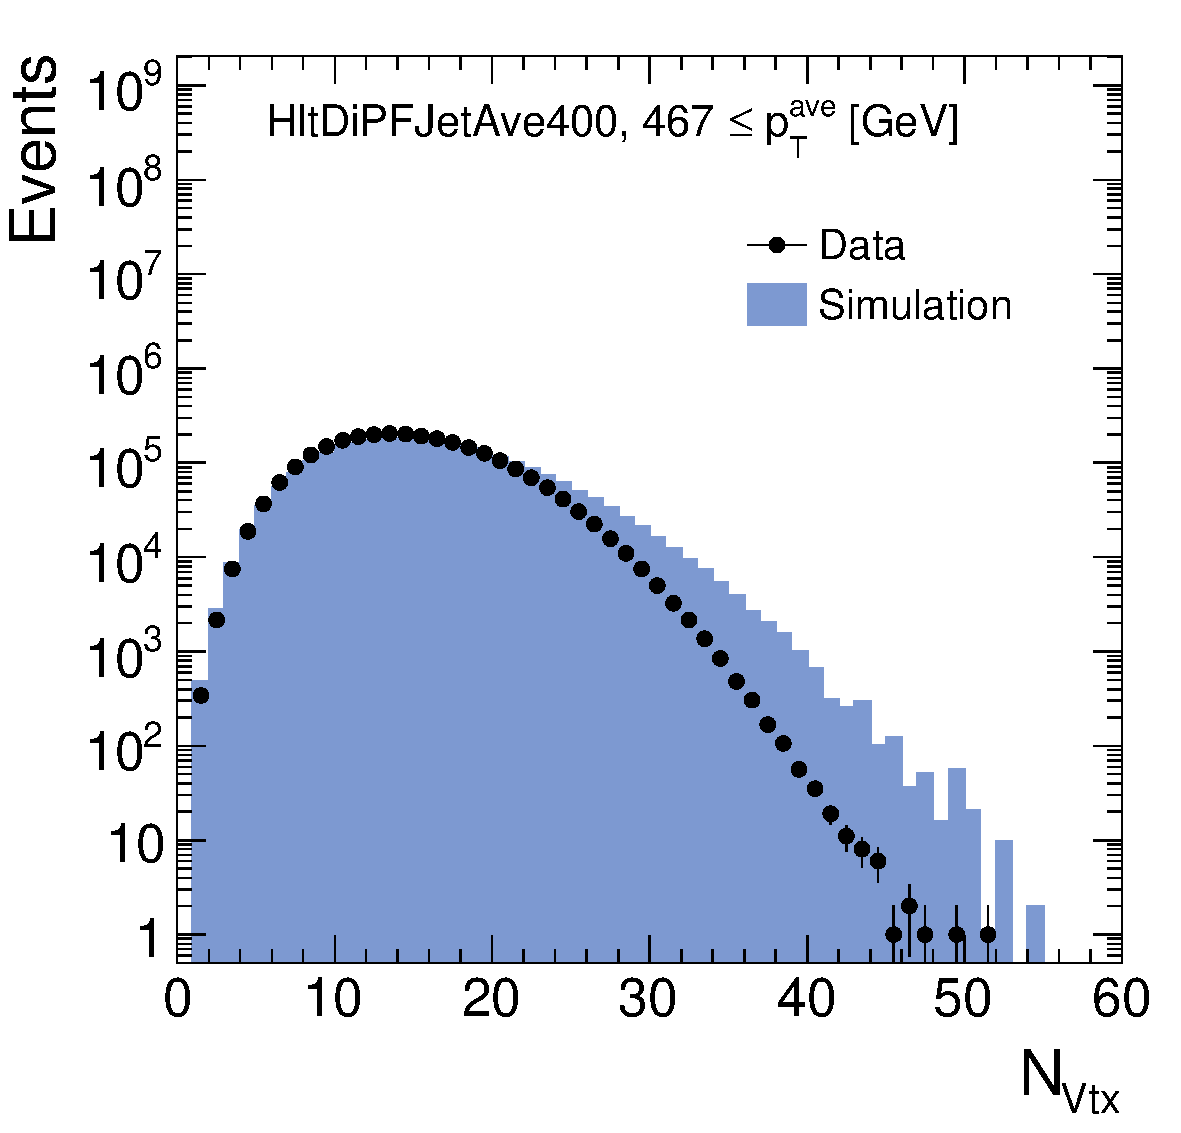
\includegraphics[width=0.49\textwidth]{figures/NVtx_HltDiPFJetAve400_AfterTriggerSelection.pdf} &
                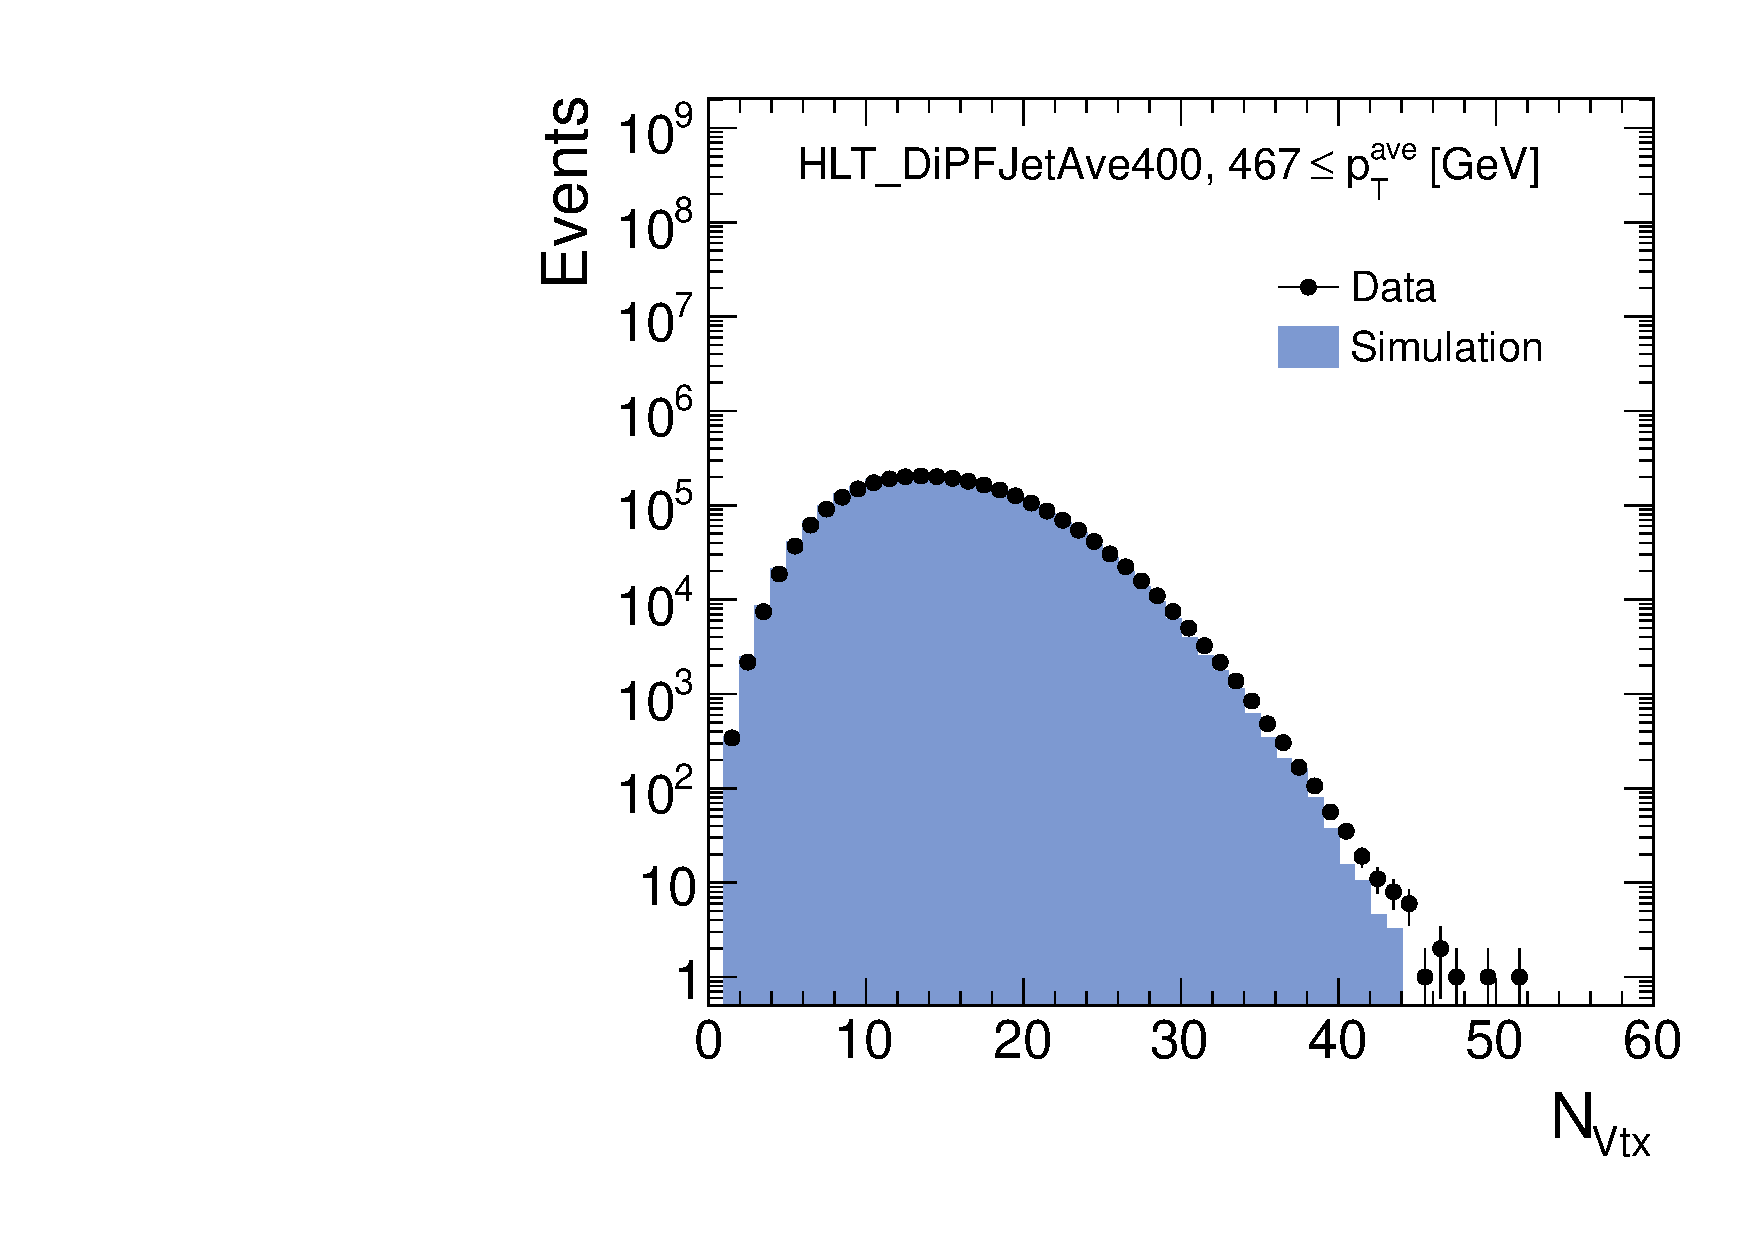
\includegraphics[width=0.49\textwidth]{figures/NVtx_HltDiPFJetAve400_AfterPUReweighting.pdf}
  \end{tabular}
  \caption{Distribution of number of primary vertices in data (black dots) and simulation (blue histogram) before (\textit{left}) and after (\textit{right}) reweighting of the pileup scenario in simulation for trigger path HltDiPFJetAve400.}
  \label{fig:pu_reweight}
\end{figure}
Thus, each trigger path collected different amounts of data and consequently also the pileup distribution differs per trigger. Hence, the reweighting of the pileup scheme is done for each trigger path individually. Depending on the offline \ptave, a simulated event can be unambigously assigned to the corresponding trigger path, which is fully efficient for that particular \pt range, and reweighted to that particular pileup scenario. Since the number of primary vertices in the event is a measure for the pileup activity, the success of the reweighting procedure can be checked by comparing the distribution of the number of primary vertices in data and simulation before and after reweighting, respectively. Such a comparison is shown in Fig.~\ref{fig:pu_reweight} for the trigger path with the highest \ptave threshold. The primary vertex distributions show a good agreement after the application of the reweighting procedure, especially in the bulk of the distribution. Corresponding distributions of other trigger paths used in the analysis are shown in App.~\ref{app:jer_pu_reweight}. The pileup weight is considered as a multiplicative factor for each simulated event. \\
In order to account for the dependence of the resolution on the transverse momentum and $\eta$, the asymmetry distributions are derived for various intervals of $|\eta|$ and $\pt^\mathrm{ave}$. These are summarized in Tab.~\ref{tab:binning}. The \ptave intervals are chosen in correspondence to the \ptave values for which the different triggers become fully efficienct. If a trigger path provides enough statistical precision, the interval is separated into two. This definition of \ptave intervals ensures that all events in one \ptave interval are selected by the same trigger. The same interval boundaries are chosen for simulated events as well. The $|\eta|$ intervals are chosen to reflect the actual detector geometry. The most central part of the detector is covered by $ 0.0 < |\eta| < 0.5$, $0.5 < |\eta| < 1.1$ while the transition region, where the ECAL ends, is separated into an individiual bin $ 2.8 < |\eta| < 3.2$. The forward detector is covered by one large bin $|\eta| = 3.2 - 5.0$ mainly due to the small number of available events. In order to allow the application of Eq.~\ref{eq:asymm} for the determination of the resolution, both leading jets are required to belong to the same $|\eta|$ interval $\Delta |\eta|$
\begin{equation}
 \Delta |\eta|_{\mathrm{jet},1} = \Delta |\eta|_{\mathrm{jet},2}
\end{equation}
\begin{table}[!t]
\centering
\caption{Overview of the $|\eta|$ and $\pt^\mathrm{ave}$ interval boundaries used for the resolution measurement.}
\label{tab:binning}
\makebox[\linewidth]{
\begin{tabular}{c}
\multicolumn{1}{c}{} \\
\toprule
 $|\eta|$ \\
 0.0, 0.5, 1.1, 1.7, 2.3, 2.8, 3.2, 5.0 \\
\midrule
$\pt^\mathrm{ave}$ [GeV] \\
62, 107, 175, 205, 242, 270, 310, \\
335, 379, 410, 467, 600, 1000, 2000 \\
\bottomrule
\end{tabular}}
\end{table} 
To account for the $\alpha$-dependence of the measured asymmetry distributions, the \ptave and $|\eta|$ intervals are further subdivided in various $\alpha$ intervals. These are chosen such that each $\alpha$ interval ranges from $\alpha = 0.0$ to a particular upper boundary $\alpha_\mathrm{max}$. The respective upper boundaries of the $\alpha_\mathrm{max}$ intervals are $0.1, 0.125, 0.15, 0.175, 0.2, 0.225, 0.25$. This inclusive definition of the $\alpha$ intervals implicates that one specific event might be assigned to more than one $\alpha$ bin. \\
The resulting inclusive $\pt^\mathrm{ave}$ spectrum after applying the the described selection is shown for data and simulationin Fig.~\ref{fig:ptave_spec}. The \pt spectra of the first three leading jets are shown as well. The number of simulated events in each trigger $\pt^\mathrm{ave}$ interval is normalized to the respective integral in data. It is visible that the shapes of the spectra in data and simulation agree well. Furthermore, the effect of the pre-scales applied to the low-\ptave-threshold triggers is nicely visible resulting in the sawtooth-shaped \ptave-spectrum.  
\begin{figure}[!tp]
  \centering
  \begin{tabular}{cc}
                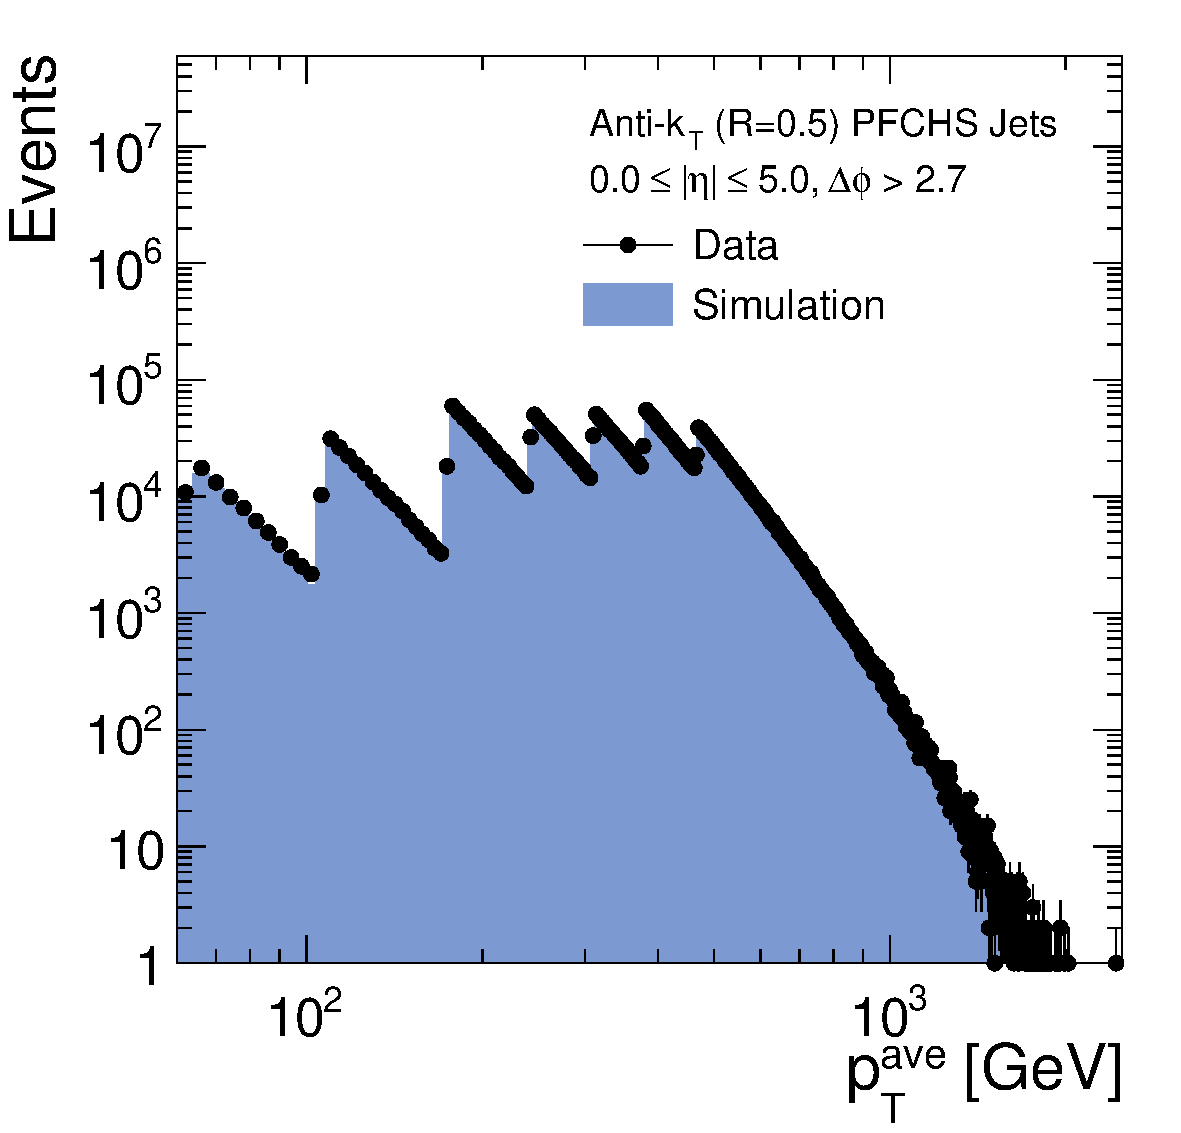
\includegraphics[width=0.49\textwidth]{figures/PtAve__AfterAsymmHistos.pdf} &
                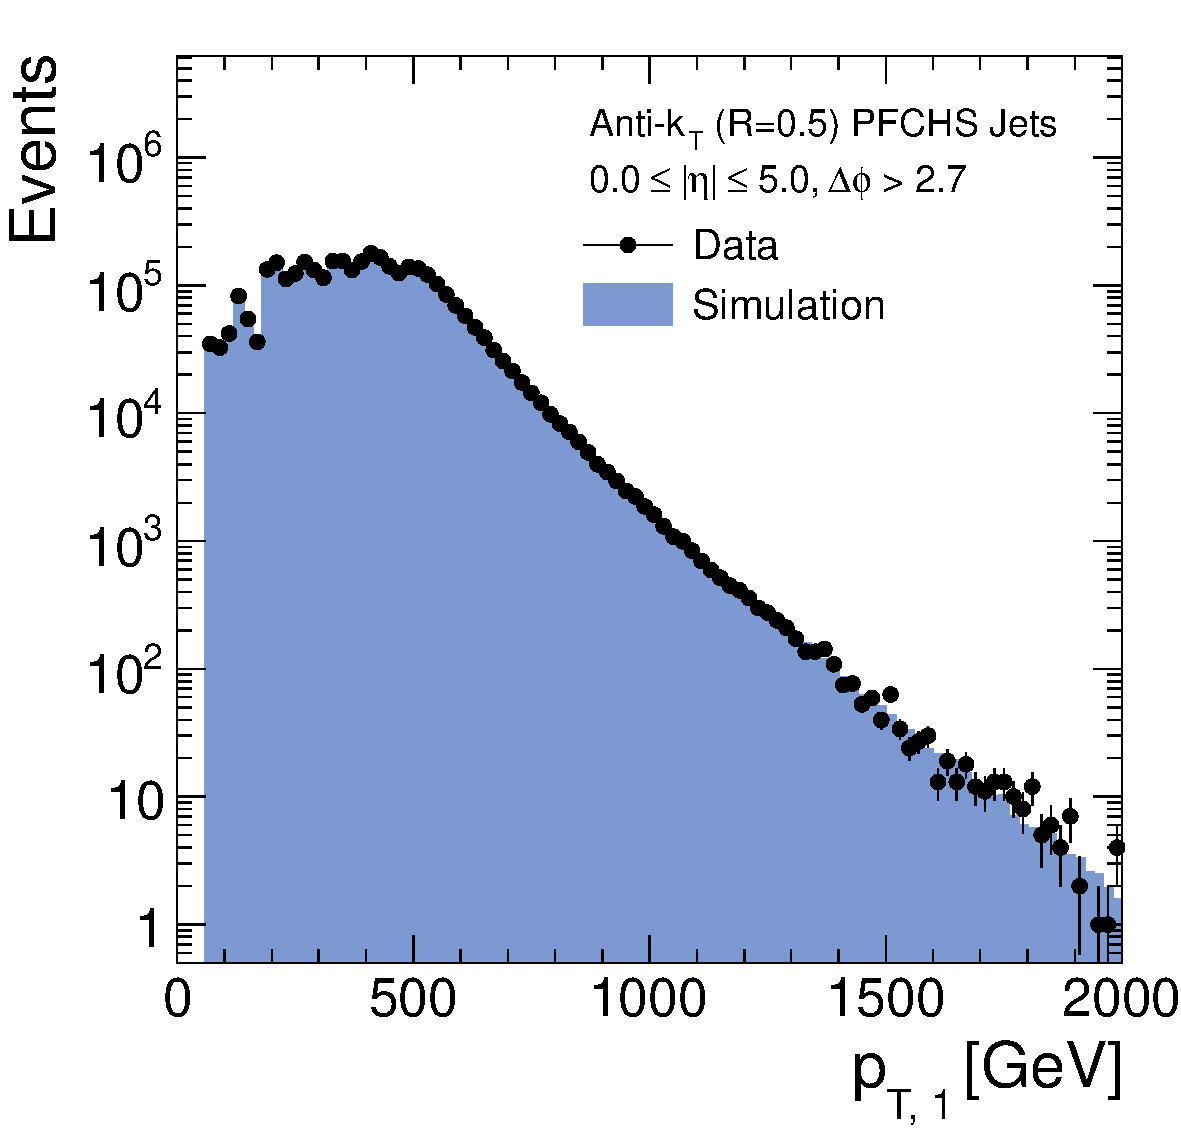
\includegraphics[width=0.49\textwidth]{figures/Jet1Pt__AfterAsymmHistos.pdf} \\
                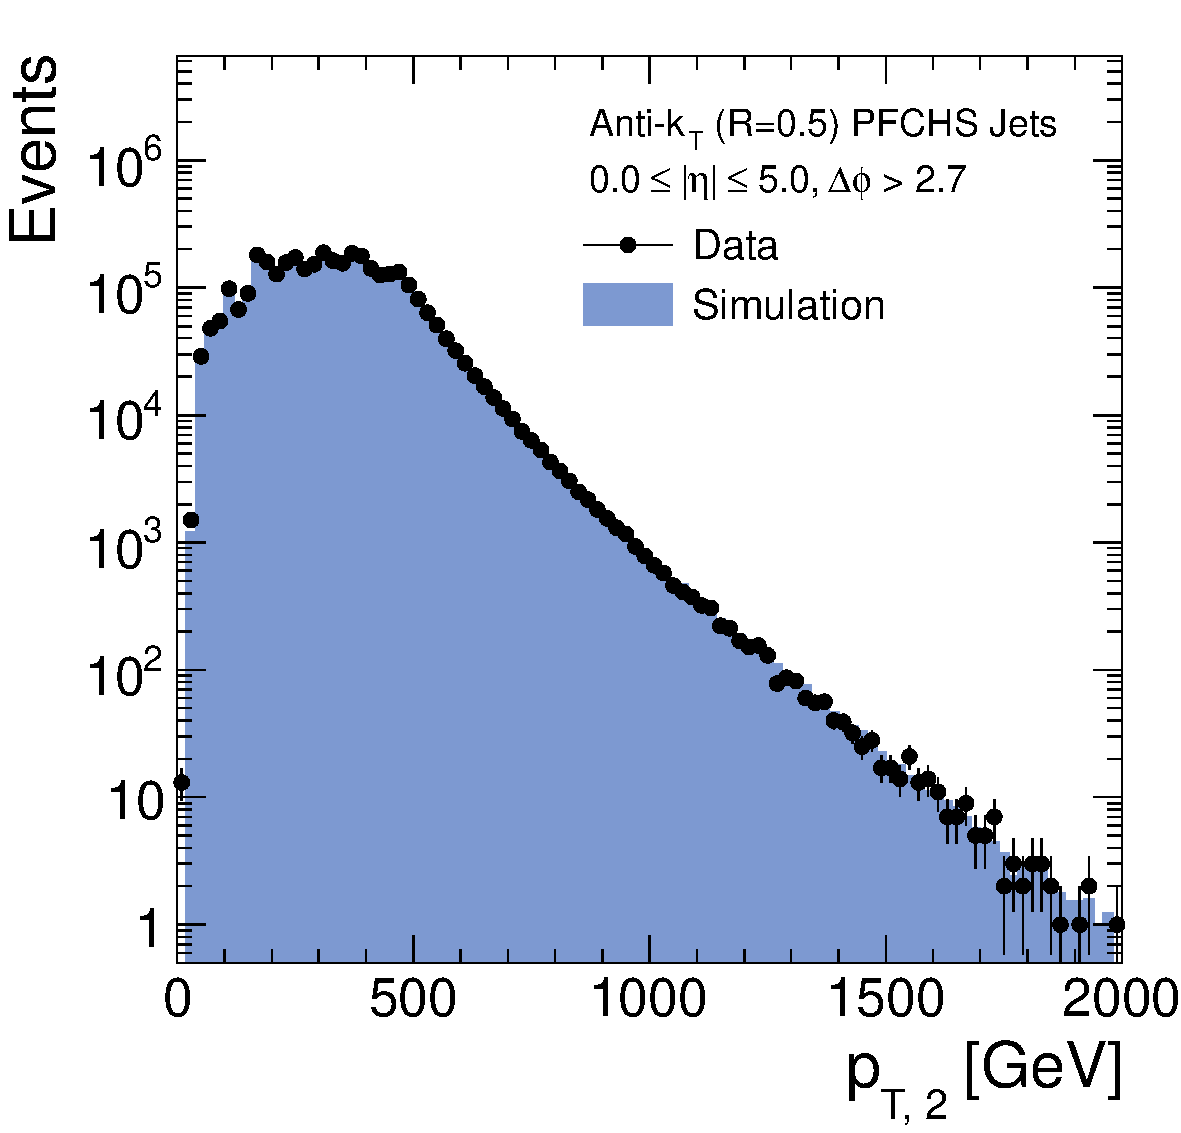
\includegraphics[width=0.49\textwidth]{figures/Jet2Pt__AfterAsymmHistos.pdf} &
                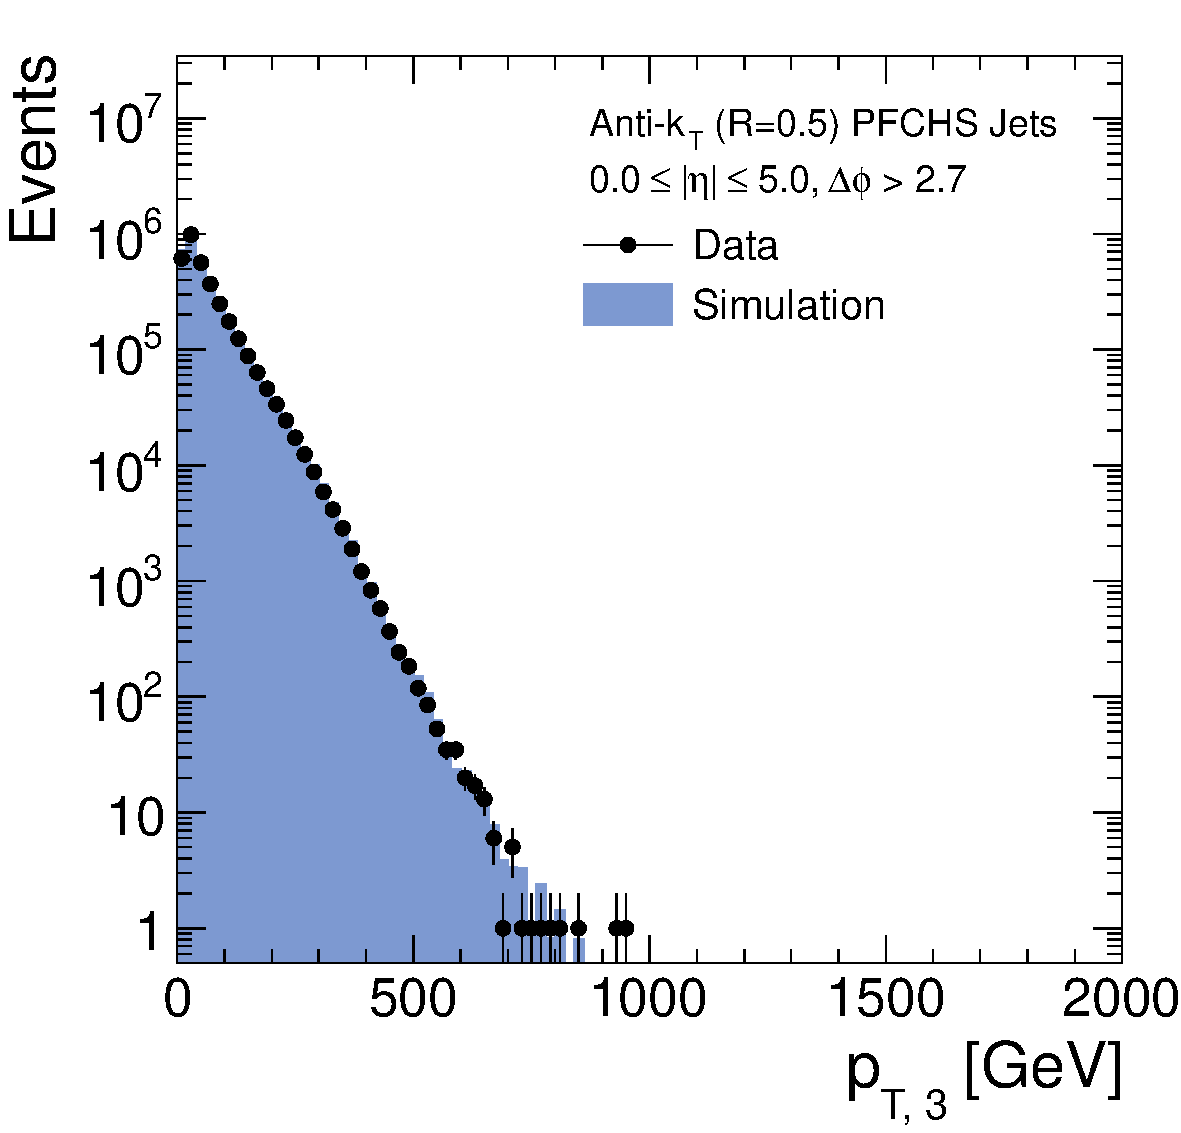
\includegraphics[width=0.49\textwidth]{figures/Jet3Pt__AfterAsymmHistos.pdf}

  \end{tabular}
  \caption{Inclusive $\pt^\mathrm{ave}$ spectrum of events after the total selection in data and in simulation (\textit{top left}), leading jet \pt (\textit{top right}), subleading jet \pt (\textit{bottom left}) and third jet \pt (\textit{bottom right}).}
  \label{fig:ptave_spec}
\end{figure}
\\
Finally, some example asymmetry distributions obtained after the described selection are depicted in Fig.~\ref{fig:asymm_dists} for data and simulated events. They have been obtained using Eq.~\ref{eq:asymmdef}. Instead of randomly assigning the first and second jet, the absolute value of the asymmetry is used. The effect that the asymmetry distribution gets broadened for larger values of $\alpha$ is visible when comparing the distributions in the top and the bottom row. In order to get a robust estimate of the asymmetry width, only asymmetry distributions with at least 100 events in the specified \ptave, $\eta$ and $\alpha$ intervals are considered for the analysis. 
\begin{figure}[!tp]
  \centering
  \begin{tabular}{cc}
                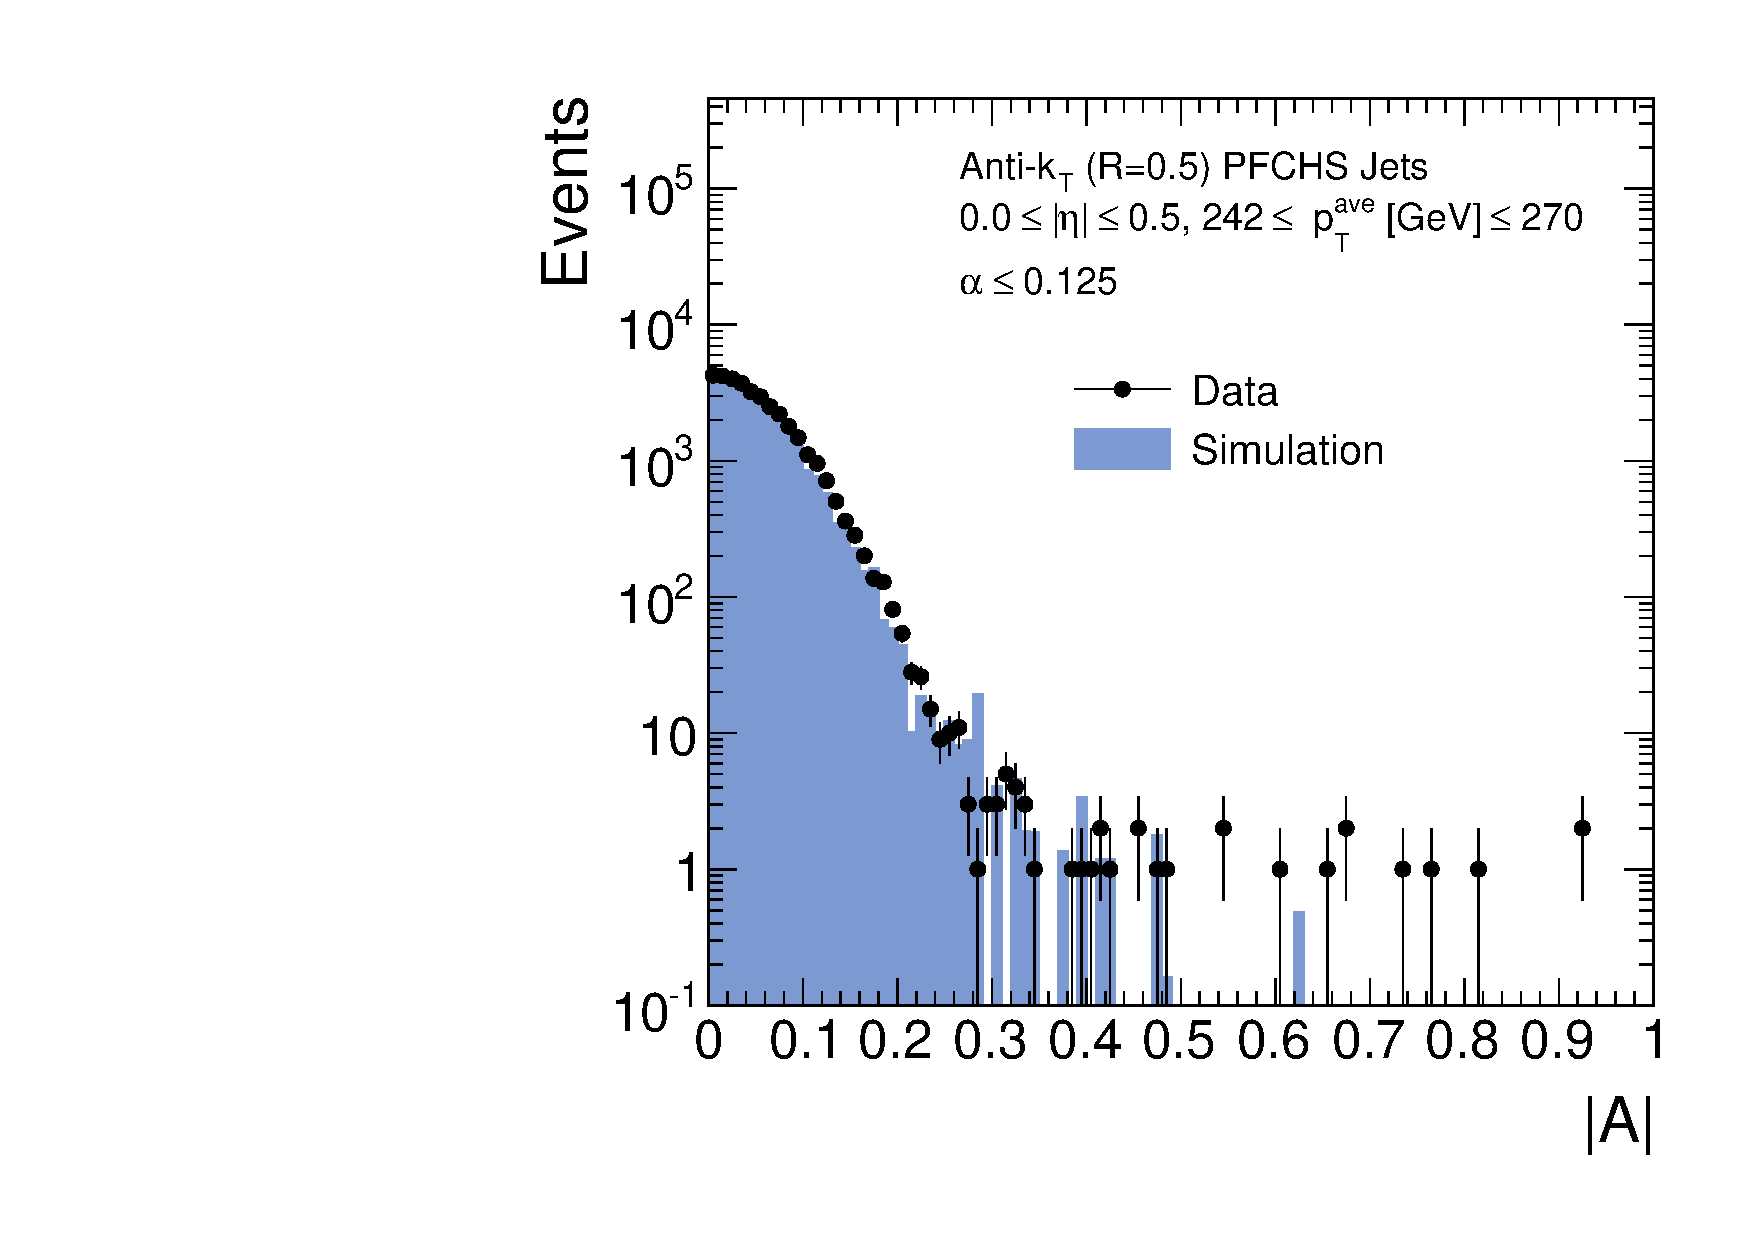
\includegraphics[width=0.49\textwidth]{figures/AsymmHistos_Eta0_pt4_alpha1_final_nominal_v4b.pdf} &
                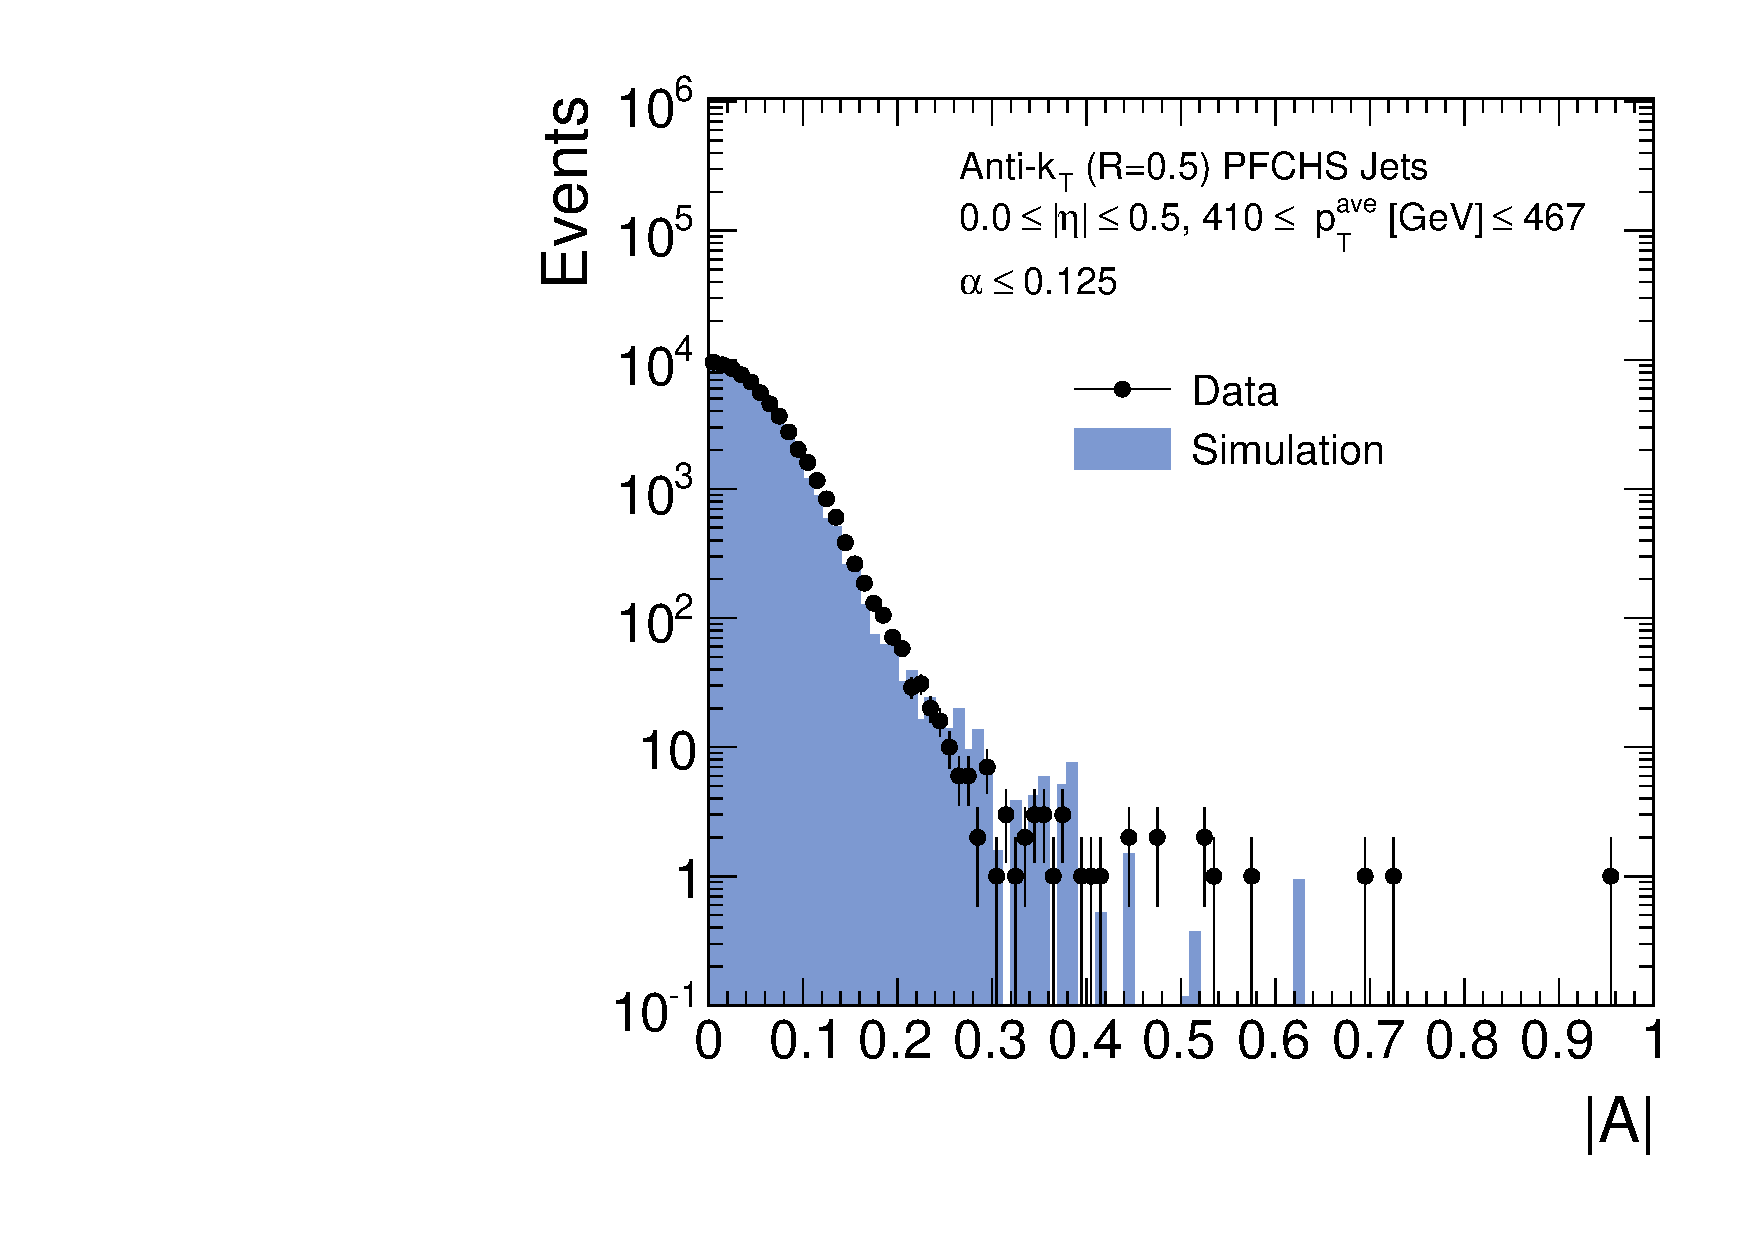
\includegraphics[width=0.49\textwidth]{figures/AsymmHistos_Eta0_pt9_alpha1_final_nominal_v4b.pdf} \\ 
                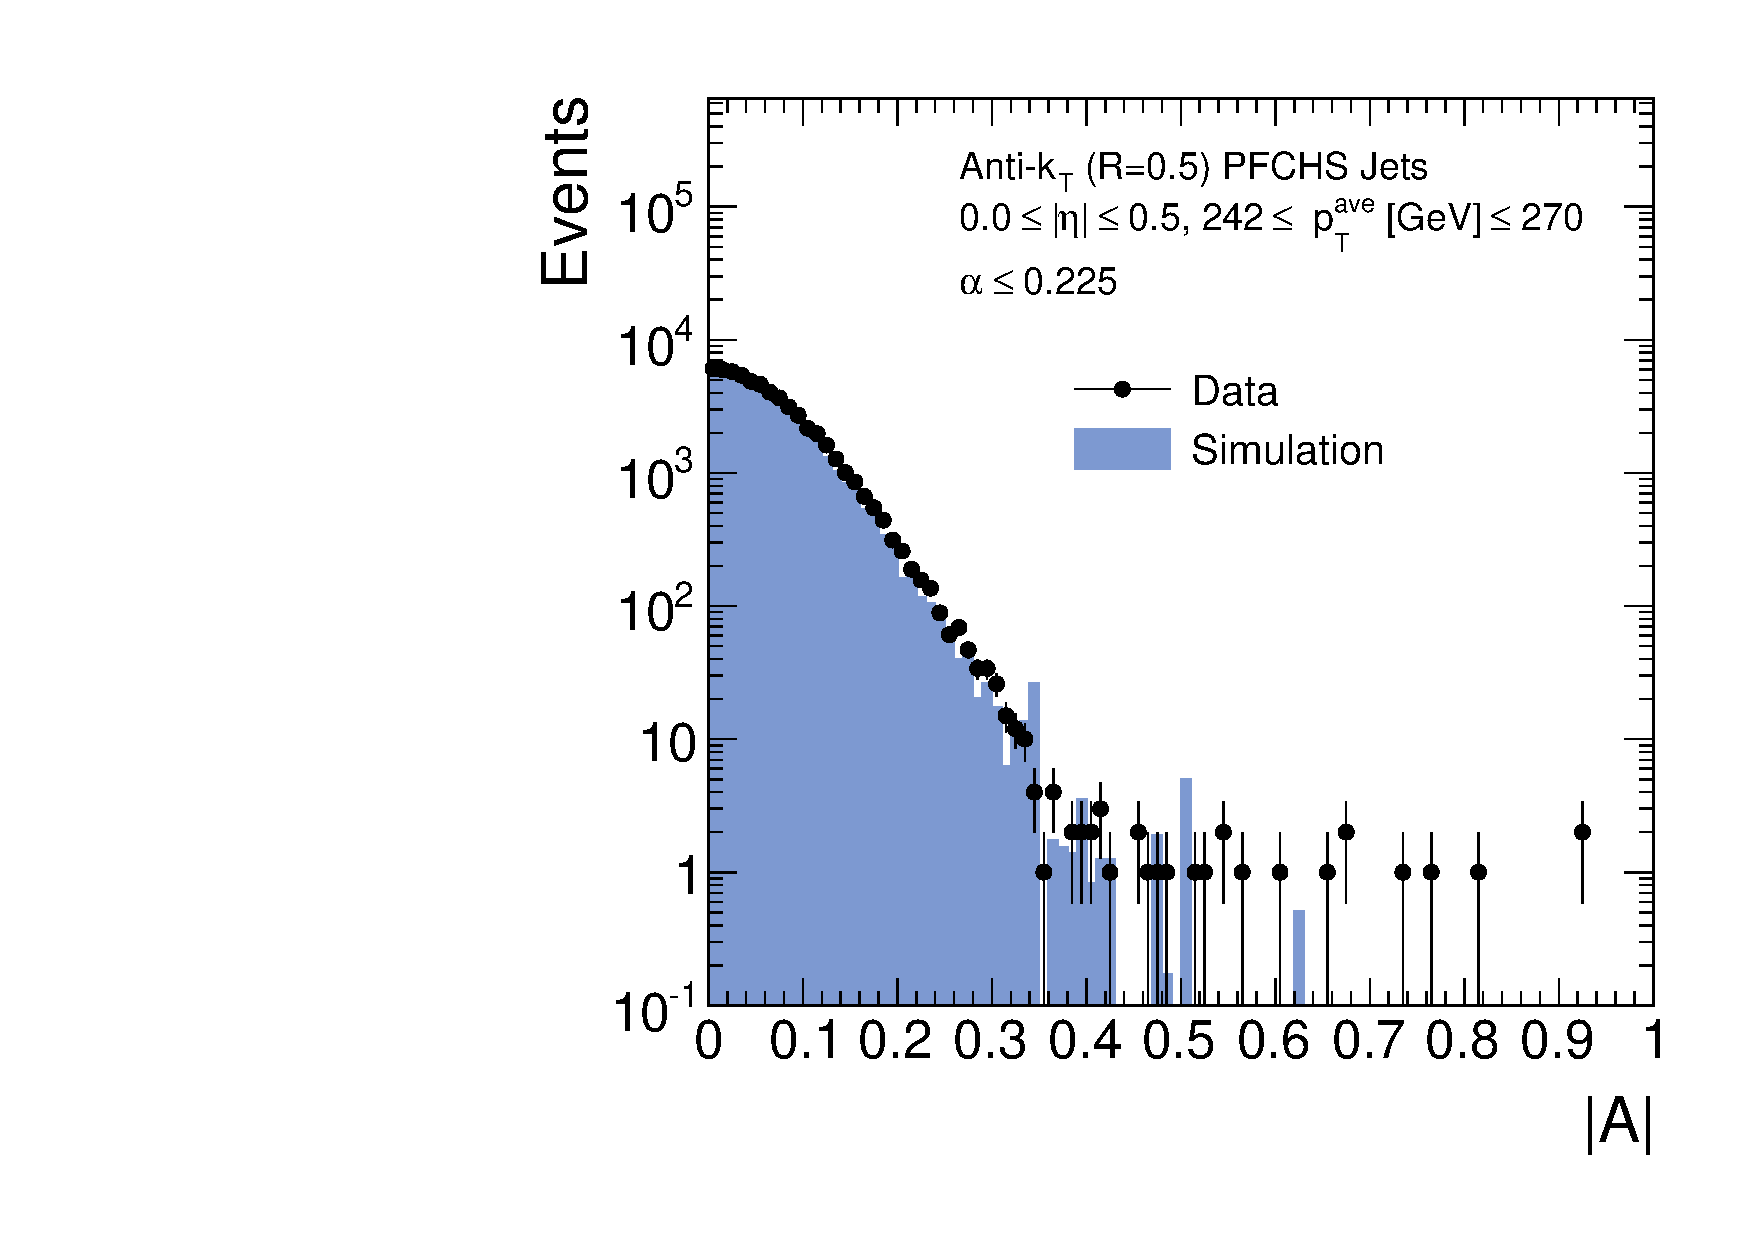
\includegraphics[width=0.49\textwidth]{figures/AsymmHistos_Eta0_pt4_alpha5_final_nominal_v4b.pdf} &
                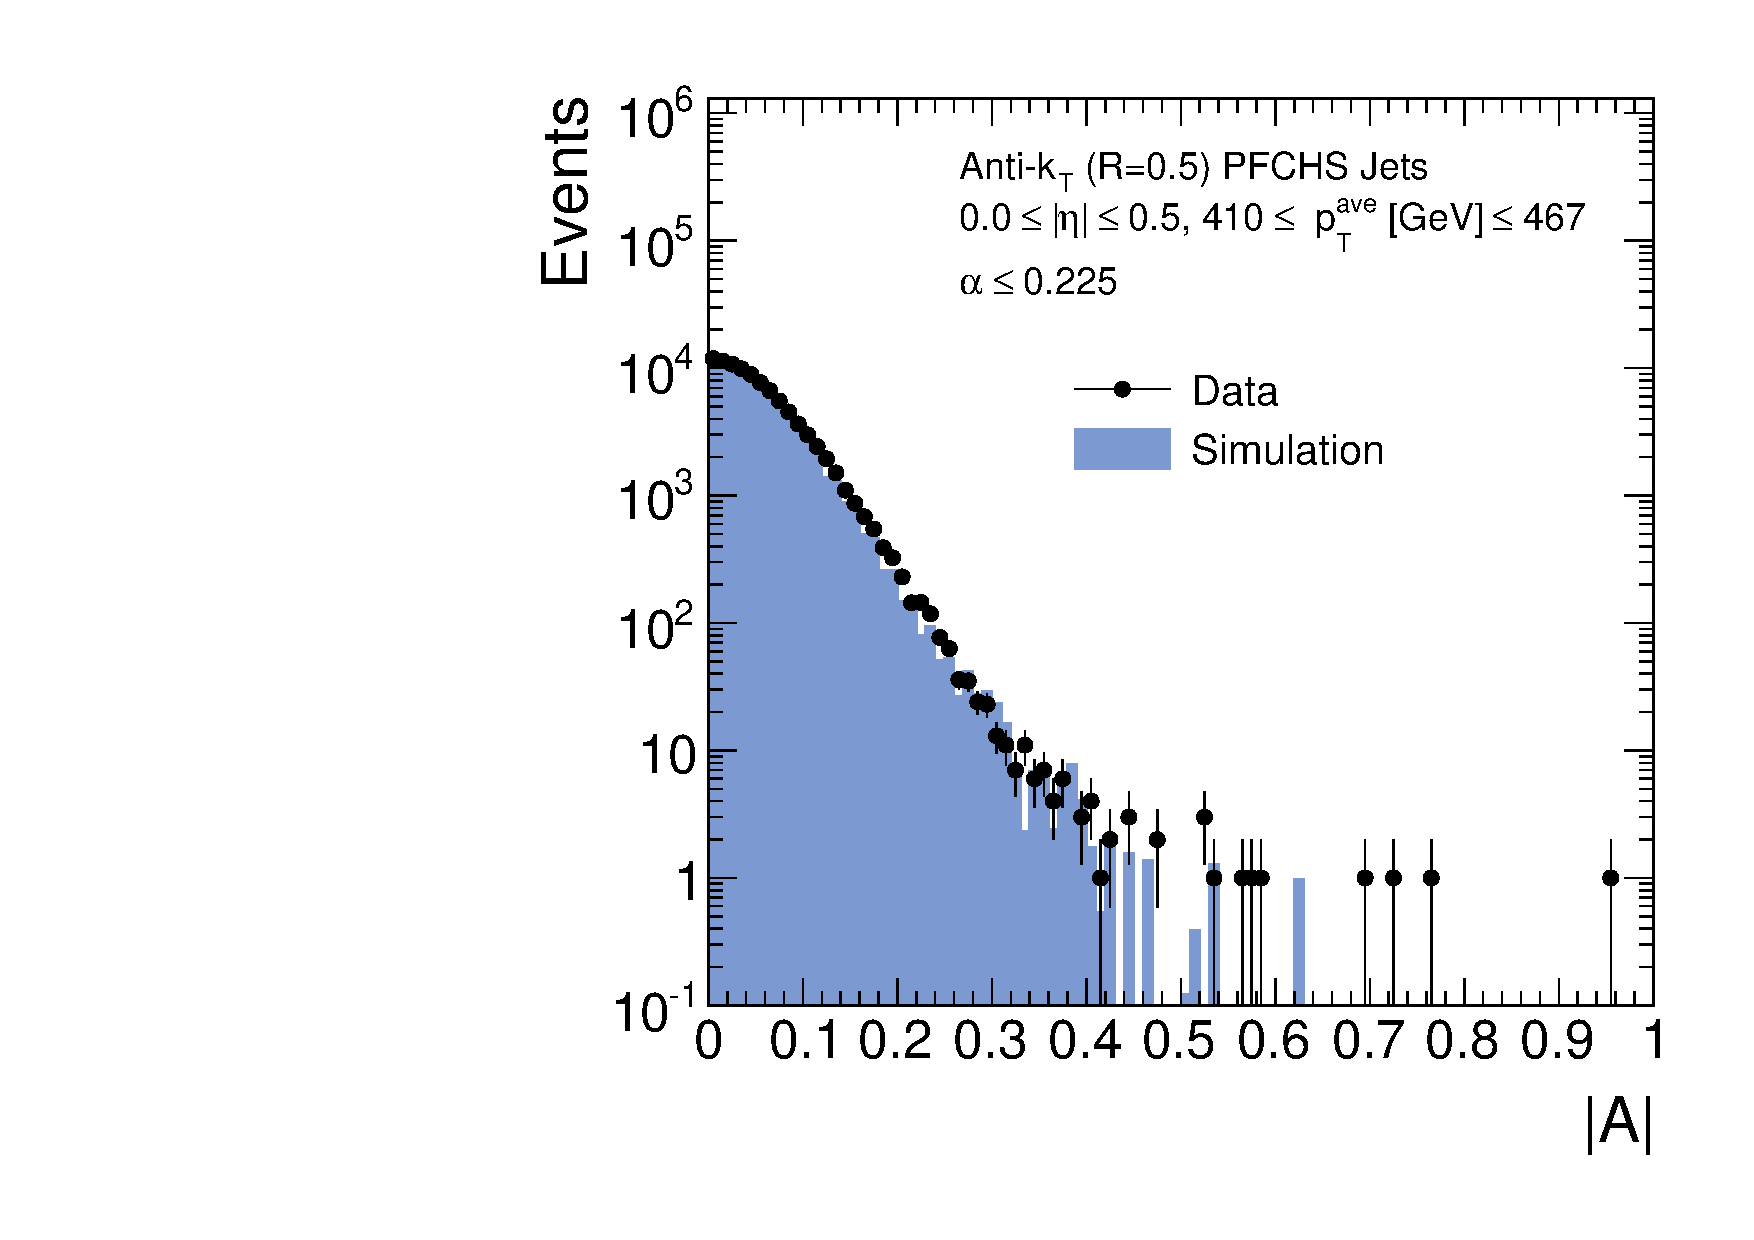
\includegraphics[width=0.49\textwidth]{figures/AsymmHistos_Eta0_pt9_alpha5_final_nominal_v4b.pdf}
  \end{tabular}
  \caption{Some example asymmetry distributions for the lowest $|\eta|$ region, two medium $\pt^\mathrm{ave}$ intervals and for a low (\textit{top}) and a high (\textit{bottom}) $\alpha$ interval.}
  \label{fig:asymm_dists}
\end{figure}

\section{Definition of the Asymmetry Width}
\label{sec:jer_asymm_width_def}
As the measurement of the resolution in collision data is based on the width of the dijet asymmetry distribution, a proper definition of the asymmetry width is needed.\\
From the tails of the jet response, events with large asymmetries can emerge leading to non-Gaussian tails in the asymmetry distributions. These tails have to be rejected in the calculation of the asymmetry width in order to avoid a bias of the measurement. Hence, the asymmetry width has to be defined such that the core part of the distribution is described. Since the core of the asymmetry distribution is expected to be Gaussian-shaped, a proper description of the asymmetry core can be tested by comparing the actual asymmetry histogram to a Gaussian function. The standard deviation of the Gaussian function can be chosen according to different definitions of the width of the asymmetry distribution and so the definition of the asymmetry width can be identified which features a good description of the asymmetry distribution by a corresponding Gaussian function. \\
\begin{figure}[!htp]   
  \centering
  \begin{tabular}{cc}
                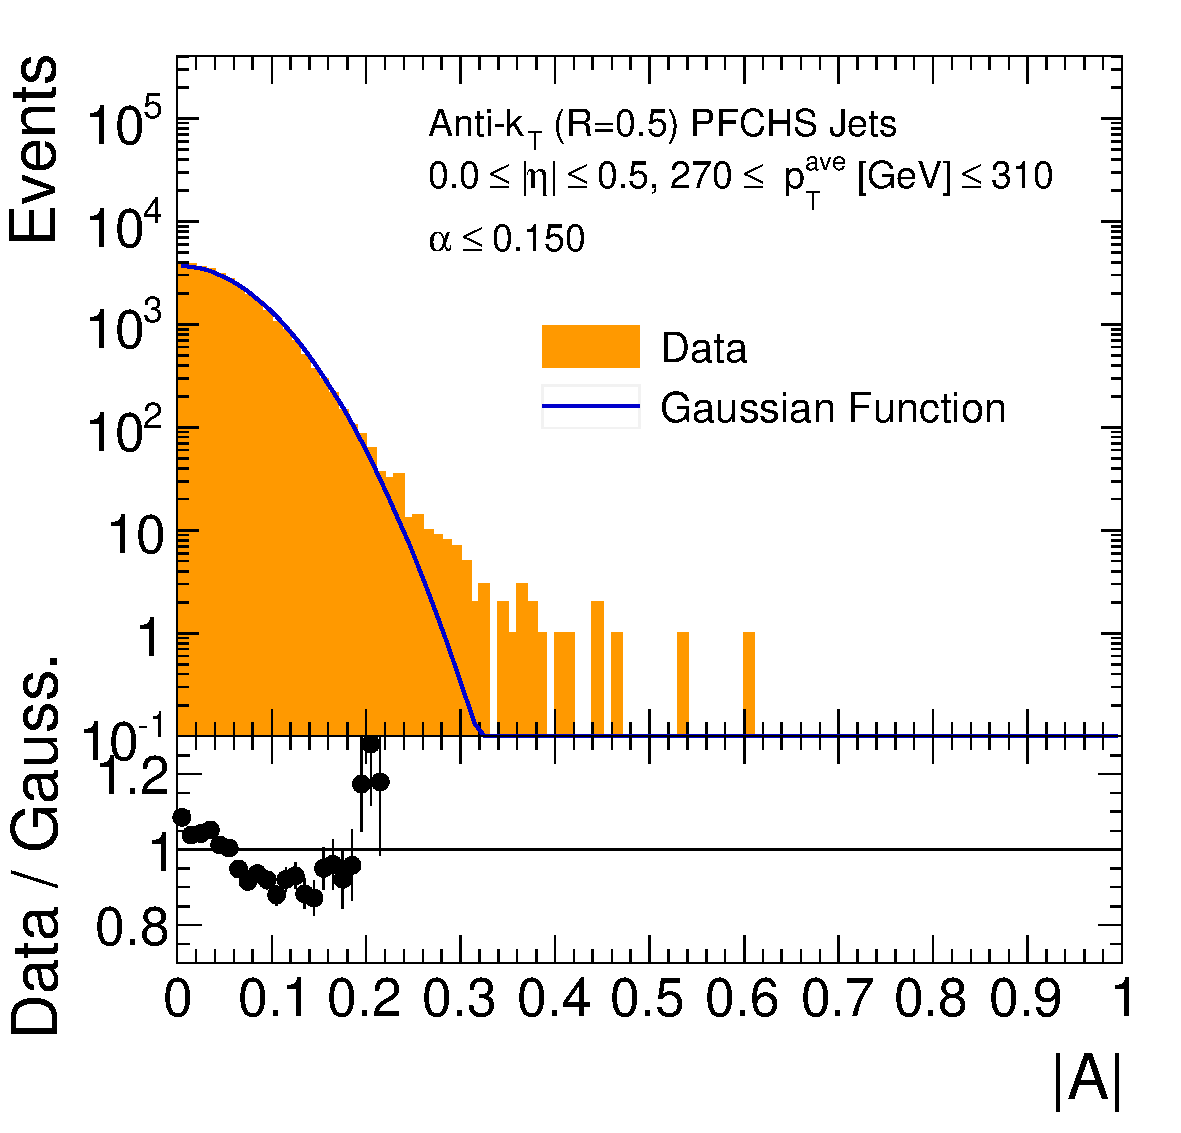
\includegraphics[width=0.49\textwidth]{figures/AsymmHistosDataWithRatio_Eta0_pt5_alpha2_final_nominal_NoTruncation_v4.pdf} &
                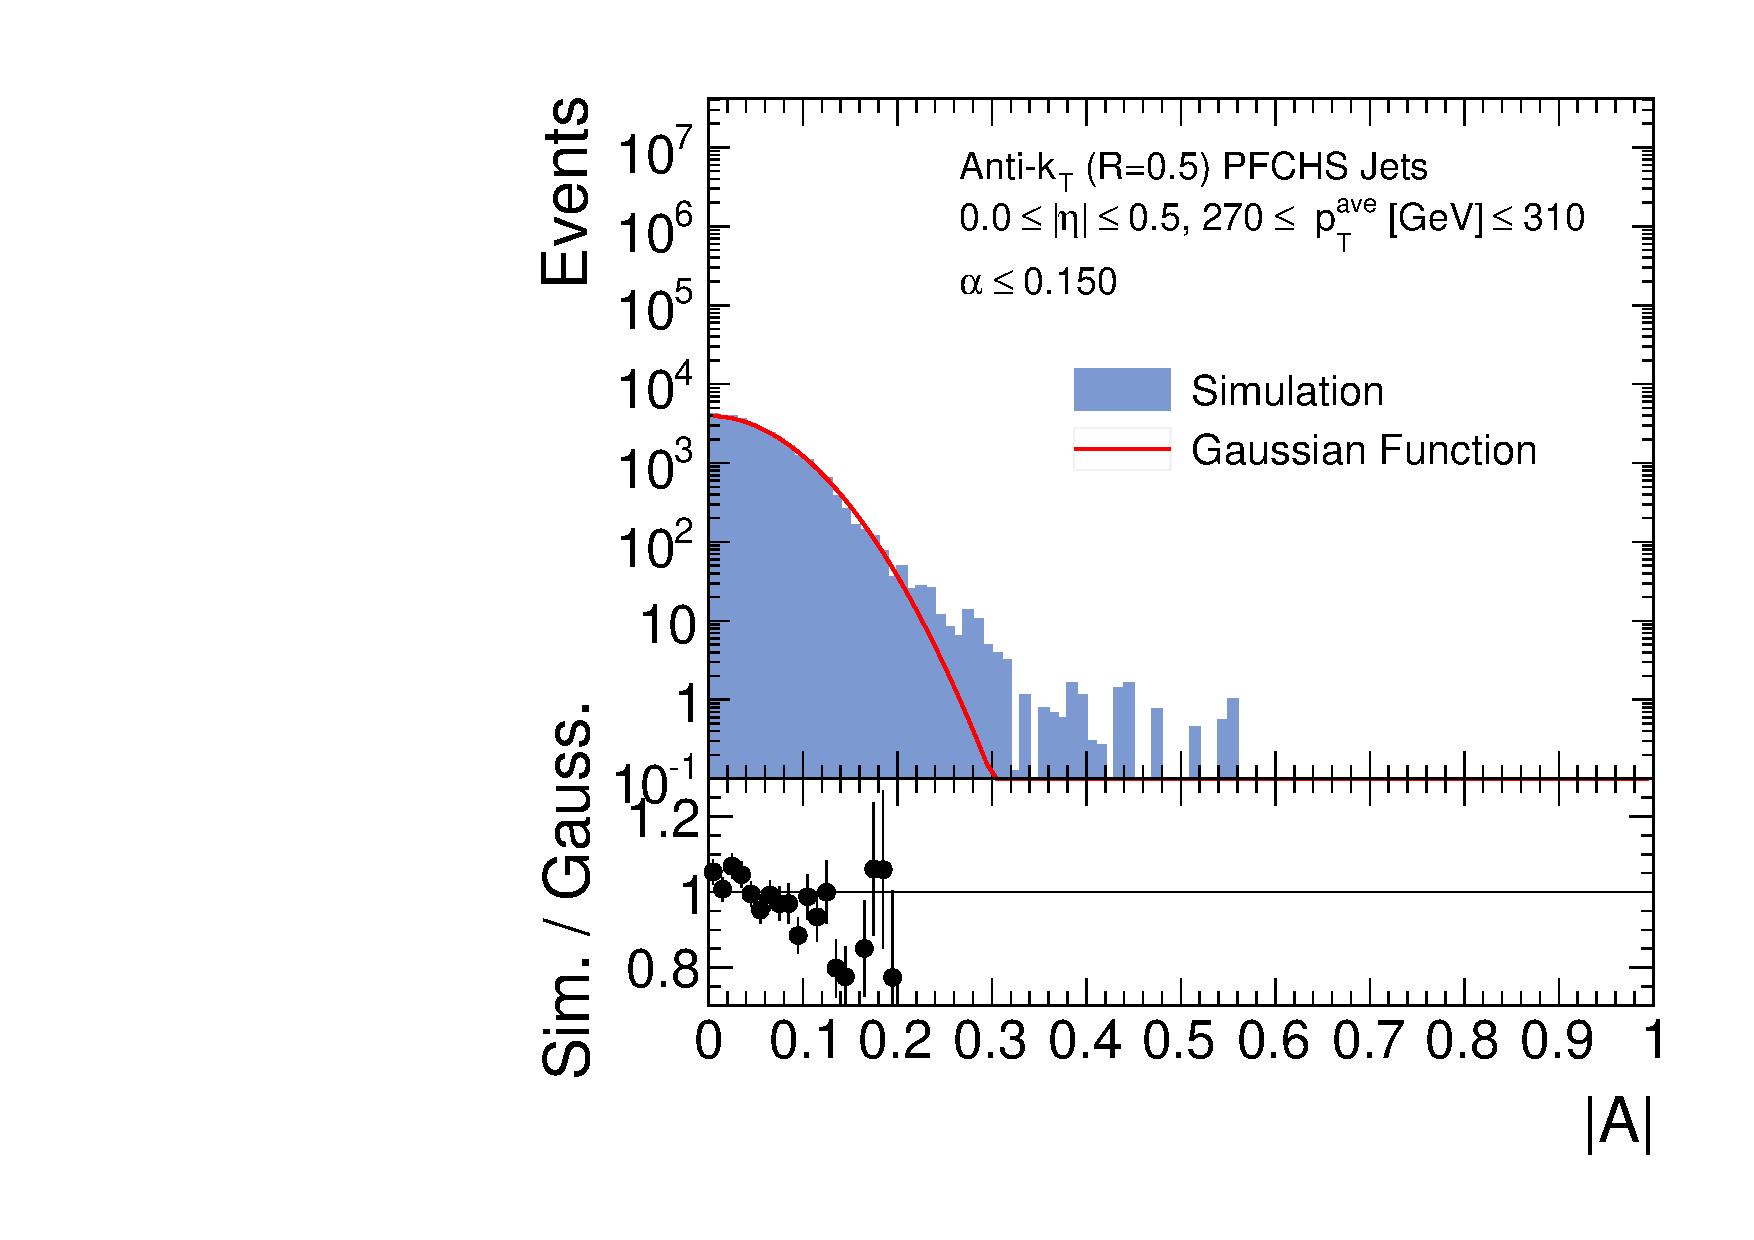
\includegraphics[width=0.49\textwidth]{figures/AsymmHistosSimWithRatio_Eta0_pt5_alpha2_final_nominal_NoTruncation_v4b.pdf} \\ 
                \includegraphics[width=0.49\textwidth]{figures/AsymmHistosDataWithRatio_Eta0_pt5_alpha2_final_nominal_v4.pdf} &
                \includegraphics[width=0.49\textwidth]{figures/AsymmHistosSimWithRatio_Eta0_pt5_alpha2_final_nominal_v4b.pdf} \\
                \includegraphics[width=0.49\textwidth]{figures/AsymmHistosDataWithRatio_Eta0_pt5_alpha2_final_nominal_95Truncation_v4.pdf} &
                \includegraphics[width=0.49\textwidth]{figures/AsymmHistosSimWithRatio_Eta0_pt5_alpha2_final_nominal_95Truncation_v4b.pdf} \\
  \end{tabular}
  \caption{Asymmetry distributions for data (\textit{left}) and simulation (\textit{right}) compared to Gaussian distributions obtained with standard deviations corresponding to 0\% truncation (\textit{top}), 1.5\% truncation (\textit{middle}) and 5\% truncation (\textit{bottom}) of the respective upper tail.}
  \label{fig:asymm_width}
\end{figure}
The width of the asymmetry is determined by taking the whole distribution into account or by truncating a certain percentage of the tail regions. Thus, the asymmetry width is calculated as truncated root-mean-square
\begin{equation}
 \sigma_\mathrm{A} = \mathrm{RMS}_{t\%} = \sqrt{\frac{1}{\sum_{i} y_i} \sum_{i} y_i \cdot A_i^2}  
 \label{eq:truncated_rms}
\end{equation} 
where $y_i$ denotes the frequency of the asymmetry value $A_i$ and the sum over $i$ includes all values such that the total asymmetry distribution is covered from zero up to a percentage $t$. Assuming a normal distribution, the statistical uncertainty is given by
\begin{equation}
\Delta \sigma_\mathrm{A} = \Delta \mathrm{RMS}_{t\%} = \frac{\mathrm{RMS}_{t\%}}{\sqrt{\, 2 \cdot n_\mathrm{eff}}} \,
\end{equation} 
with the number of effective entries $n_\mathrm{eff}$\footnote{In case of an unweighted histogram, $n_\mathrm{eff}$ is equivalent to the number of histogram entries. However, for a weighted histogram, as \eg in simulation, $n_\mathrm{eff}$ corresponds to the hypothetical number of unweighted entries a histogram would need, in order to have the same statistical power as the weighted histogram.} in the specified (\ptave, $|\eta|$, $\alpha$)-interval. The truncation is chosen such that the whole distribution, $98.5\%$ or only $95\%$ are considered. A comparison of the asymmetry distributions and Gaussian functions where the standard deviation has been set to the value of the determined asymmetry width is illustrated in Fig.~\ref{fig:asymm_width} for a certain $|\eta|$, $\pt^\mathrm{ave}$ and $\alpha$ interval. It is visible that the core part of the asymmetry distribution can in good approximation be described by a Gaussian function when choosing $\mathrm{RMS}_{98.5\%}$ as the asymmetry width (\cf middle row in Fig.~\ref{fig:asymm_width}). Hence, this is the default definition of the asymmetry width used for this measurement. It is chosen to be the same for data events as well as for simulated events.  

\section{Corrections to the Dijet Asymmetry}
\label{sec:jer_corrections}
The fundamental relation between the width of the asymmetry distribution and the jet energy resolution as expressed in Eq.~\ref{eq:asymm} holds in this form only for the case of an ideal dijet topology. In real collision events, various effects occur that disturb the exact balance of the two jets as discussed in Section~\ref{sec:jer_application}. Such effects can be soft radiation or additional jets originating from the hard scattering. They lead to momentum imbalance in the event and hence broaden the measured asymmetry distribution which consequently also results in an increased measured jet resolution. In order to determine the intrinsic resolution, the measured asymmetry width has to be corrected for such effects. These corrections are explained in the following Sections~\ref{subsec:jer_corrections_alpha} and~\ref{subsec:jer_corrections_pli}.

\subsection{Correction for Additional Jet Activity}
\label{subsec:jer_corrections_alpha}
%In addition to the two jets originating from the hard interaction, further jets can occur in an event from the emission of additional partons. The additional jet activity in the event is quantified by $\alpha$ introduced in Eq.~\ref{eq:alpha} which is the fractional \pt of the third jet. The impact from jets beyond the third one is neglected since there impact is expected to be small due to the strongly decreasing jet-production cross-section. \\
The imbalance contribution arising from additional jet activity is taken care of by an extrapolation procedure. As described in Section~\ref{subsec:jer_sel_cuts}, the asymmetry distribution is calculated for several intervals in $|\eta|$ and $\pt^\mathrm{ave}$ with different selections on the maximum value of $\alpha$ ($=\alpha_{max}$). For each of these individual selections, the width of the asymmetry is determined as stated in Section~\ref{sec:jer_asymm_width_def}. The measured values of $\sigma_{A}(\alpha_{max})$ are extrapolated to $\alpha_{max} \rightarrow 0$ assuming a linear behaviour. Thus, the measured asymmetry widths in one particular ($\pt^\mathrm{ave}$, $|\eta|$, $\alpha$)-interval are fitted with a linear function. The $y$-intercept of the fitted linear function represents the resolution without further jet activity in the event. The statistical uncertainty is given by the respective fit uncertainty for the intercept. \\
The extrapolation procedure for two exemplative $|\eta|$ and $\pt^\mathrm{ave}$ intervals is illustrated in Fig.~\ref{fig:extrapol}. The performed extrapolation fits for all other non-empty intervals are shown in App.~\ref{app:extrapolations}. 
\begin{figure}[!tp]
  \centering
  \begin{tabular}{cc}
                \includegraphics[width=0.49\textwidth]{figures/Extrapol_Eta0_pt4_final_nominal_v4.pdf} &
                \includegraphics[width=0.49\textwidth]{figures/Extrapol_Eta0_pt9_final_nominal_v4.pdf}
  \end{tabular}
  \caption{Two example extrapolations of measured values for $\sigma_\mathrm{A}$ in data (black) and simulation (red) to obtain the asymmetry width for zero additional jet activity.}
  \label{fig:extrapol}
\end{figure}
\\
As stated in Section~\ref{subsec:jer_sel_cuts}, the selection is performed in inclusive intervals of $\alpha < \alpha_\mathrm{max}$. This results in a correlation of the measured values of $\sigma_\mathrm{A}$ for a particular ($\pt^\mathrm{ave}$, $|\eta|$)-interval. In order to obtain a proper estimate of the statistical uncertainty, the correlation is propagated to the extrapolation fit. This approach is new with respect to previous analyses in which such correlations have not been considered in the extrapolation procedure~\cite{1748-0221-6-11-P11002, thesis:Schroeder, Aad:2012ag}. \\
More specifically this means that the measured data points are described by a linear function 
\begin{equation}
 a \cdot \alpha_\mathrm{max} + b = \sigma_\mathrm{A}(\alpha_\mathrm{max})
\end{equation}
by determining the parameters $a$ and $b$. This is done for known $\alpha_\mathrm{max}$ and $\sigma_\mathrm{A}(\alpha_\mathrm{max})$ by minimizing 
\begin{equation}
\chi^2 = dy^T \cdot C^{-1} \cdot dy
\end{equation}
with $dy = y_{\mathrm{measured}} - y_{\mathrm{predicted}}$ and the covariance matrix $C$. Consequently, the asymmetry width for vanishing additional jet activity is given by $b=\sigma_\mathrm{A}(\alpha_\mathrm{max} \rightarrow 0)$. With the assumption that all events that belong to $\alpha$ interval $i$ are also completely included in the next higher $\alpha$ interval $j$\footnote{This assumption is only almost true since the asymmetry distributions are truncated to reject non-Gaussian components and some events might not fulfill this criterion.} the covariance matrix is given by
\begin{equation}
C_{i,j}(\sigma_{A_i},\sigma_{A_j}) = (\Delta \sigma_{A_i})^2 \cdot \frac{\sigma_{A_i}}{\sigma_{A_j}} \cdot \frac{n_i}{n_j} 
\label{eq:jer_corr}
\end{equation}
where $n$ is the number of events in that particular $\alpha$ interval. A discussion regarding the derivation of that expression is summarized in App.~\ref{app:extrapol_corr}. The function minimization itself is performed with the Minuit package~\cite{Minuit}.   
\begin{figure}[!tp]
  \centering
  \begin{tabular}{cc}
                \includegraphics[width=0.49\textwidth]{figures/GoodnessOfFit_Eta0_final_nominal_v4.pdf} &
                \includegraphics[width=0.49\textwidth]{figures/GoodnessOfFit_Eta1_final_nominal_v4.pdf} \\
 %               \includegraphics[width=0.49\textwidth]{figures/GoodnessOfFit_Eta2_final_nominal_v4.pdf} &
 %               \includegraphics[width=0.49\textwidth]{figures/GoodnessOfFit_Eta3_final_nominal_v4.pdf} \\
 %               \includegraphics[width=0.49\textwidth]{figures/GoodnessOfFit_Eta4_final_nominal_v4.pdf}
  \end{tabular}
  \caption{Goodness-of-fit test for the extrapolation fits in data and simulation in the two central $|\eta|$ regions as function of $\pt^\mathrm{ave}$.}
  \label{fig:goodness-of-fit}
\end{figure}
In Fig.~\ref{fig:goodness-of-fit}, an overview of a goodness-of-fit test is shown for the extrapolation fits in data and simulation. The resulting values for $\chi^2$ over the number of degrees of freedom are shown as function of $\pt^\mathrm{ave}$ exemplary for the two central $|\eta|$ intervals. This is expected to be distributed around 1. Consequently, the fit quality is in general quite good but worsens for larger $\pt^\mathrm{ave}$ values. Since especially for higher $\pt^\mathrm{ave}$ intervals in the central $|\eta|$ regions, the statistical uncertainty is rather low, the fit is very sensitive to even small deviations from a linear behaviour which results in a minor fit quality. However, a possible non-linearity is considered in the systematic uncertainties of the measurement, as discussed in Section~\ref{sec:jer_syst_unc}.

\subsection{Correction for Particle-Level Imbalance}
\label{subsec:jer_corrections_pli}
In addition to an imbalance in dijet events caused by the presence of additional jets, an imbalance in the dijet system at particle level can also arise for instance from out-of-cone showering. This additional imbalance contribution is referred to as \textit{particle-level imbalance} (PLI) and estimated from simulation. \\
The contribution arising from the particle-level imbalance is estimated from the dijet asymmetry defined at generator level. This is defined equivalently to the asymmetry at detector level but based on generator-level jet quantities as
\begin{equation}
  \mathrm{A^{gen}} = \frac{p_\mathrm{T,1}^\mathrm{gen} - p_\mathrm{T,2}^\mathrm{gen}}{p_\mathrm{T,1}^\mathrm{gen} + p_\mathrm{T,2}^\mathrm{gen}} 
 \end{equation}
with $p_\mathrm{T,1}^\mathrm{gen}$ and $p_\mathrm{T,2}^\mathrm{gen}$ referring to the momenta of the two leading generated jets. This distribution is affected by additional parton radiation as well. Thus, the procedure to obtain $\sigma^\mathrm{gen}_\mathrm{A}(\alpha_\mathrm{max} \rightarrow 0)$ is the same as for the asymmetry at detector level. The generator asymmetry is calculated in the same ($\pt^\mathrm{ave}$, $|\eta|$, $\alpha$)-intervals as the detector-level asymmetry in order to derive the size of the particle-level imbalance for exactly the same events. The asymmetry width of the generator asymmetry is also calculated as $\mathrm{RMS}_{98.5\%}$. In order to obtain the values of $\sigma^\mathrm{gen}_\mathrm{A}$ for zero additional jet activity, the analogue extrapolation procedure is performed, as described in Sec.~\ref{subsec:jer_corrections_alpha}. Some example extrapolations are illustrated in Fig.~\ref{fig:extrapol_gen}. 
\begin{figure}[!tp]
  \centering
  \begin{tabular}{cc}
                \includegraphics[width=0.49\textwidth]{figures/Extrapol_Eta0_pt4_gen_final_nominal_v4b.pdf} &
                \includegraphics[width=0.49\textwidth]{figures/Extrapol_Eta0_pt9_gen_final_nominal_v4b.pdf}
  \end{tabular}
  \caption{Two example extrapolations of measured values for $\sigma^\mathrm{gen}_\mathrm{A}$ in simulation to determine the contribution from PLI.}
  \label{fig:extrapol_gen}
\end{figure}
\\
Finally, the results of the extrapolated values for $\sigma^\mathrm{gen}_\mathrm{A}$ can be used to quantify the size of the particle-level imbalance. This is given by
 \begin{equation}
 \label{eq:pli}
 \sigma_\mathrm{PLI} = \sqrt{2} \cdot \sigma^\mathrm{gen}_\mathrm{A}(\alpha_\mathrm{max} \rightarrow 0) \, .
 \end{equation}

\subsection{Results of the Corrections to the Asymmetry}
\label{subsec:jer_corrections_results} 
The results of the various extrapolation fits to determine $ \sigma_\mathrm{A}(\alpha_\mathrm{max} \rightarrow 0)$ in data and simulation as well as for the particle-level imbalance are shown together in Fig.~\ref{fig:fit-results} as a function of $\pt^\mathrm{ave}$ for the different $|\eta|$ regions. 
\begin{figure}[!htp]
  \centering
  \begin{tabular}{cc}
                \includegraphics[width=0.49\textwidth]{figures/Extrapol_Eta0_final_nominal_v4b.pdf} &
                \includegraphics[width=0.49\textwidth]{figures/Extrapol_Eta1_final_nominal_v4b.pdf} \\
  %              \includegraphics[width=0.49\textwidth]{figures/Extrapol_Eta2_final_nominal_v4.pdf} &
  %              \includegraphics[width=0.49\textwidth]{figures/Extrapol_Eta3_final_nominal_v4.pdf} \\
  %              \includegraphics[width=0.49\textwidth]{figures/Extrapol_Eta4_final_nominal_v4.pdf}
  \end{tabular}
  \caption{Results of extrapolation fits in the two central $|\eta|$ regions as a function of $\pt^\mathrm{ave}$ for data (black), simulation (red) and particle-level imbalance (blue).}
  \label{fig:fit-results}
\end{figure}
\\
In order to obtain the jet energy resolution, the results of the extrapolated detector-level asymmetry widths are corrected for the effects from particle-level imbalance. This is done by subtracting the PLI correction in quadrature from the measured $\sigma_\mathrm{A}$ after the correction for additional jet activity 
\begin{equation}
\sigma_\mathrm{JER} =  \sqrt{2} \cdot \sigma_\mathrm{A}(\alpha_\mathrm{max} \rightarrow 0) \ominus \sigma_\mathrm{PLI} \, .
\end{equation}  
The same PLI correction is substracted both from data as well as from simulation results. As can be seen in Fig.~\ref{fig:fit-results}, the correction due to particle-level imbalance is small compared to the measured asymmetry widths. This justifies to take this correction from simulation, also for the data resolution. However, in order to account for a possible imprecise modelling of the particle-level imbalance contribution, a systematic uncertainty will be considered, as discussed in Sec.~\ref{sec:jer_syst_unc}.

\section[Determination of the Data-to-Simulation Ratio]{Determination of the Data-to-Simulation Ratio of the Jet Transverse Momentum Resolution}
\label{sec:jer_ratio_determination}
\begin{figure}[!htp]
  \centering
  \begin{tabular}{cc}
                \includegraphics[width=0.49\textwidth]{figures/ExtrapolRatio_Eta0_with_pli_final_nominal_v4b.pdf} &
                \includegraphics[width=0.49\textwidth]{figures/ExtrapolRatio_Eta1_with_pli_final_nominal_v4b.pdf} \\
                \includegraphics[width=0.49\textwidth]{figures/ExtrapolRatio_Eta2_with_pli_final_nominal_v4b.pdf} &
                \includegraphics[width=0.49\textwidth]{figures/ExtrapolRatio_Eta3_with_pli_final_nominal_v4b.pdf} \\
                \includegraphics[width=0.49\textwidth]{figures/ExtrapolRatio_Eta4_with_pli_final_nominal_v4b.pdf}
  \end{tabular}
  \caption{Ratio of the resolution in data to the resolution in the \pythia QCD sample in non-empty $|\eta|$ regions as a function of $\pt^\mathrm{ave}$ shown together with a constant fit (red line) and corresponding statistical uncertainty (grey shaded area).}
  \label{fig:ratio}
\end{figure}
After applying all corrections described in Sec.~\ref{sec:jer_corrections}, the measured resolution in data and simulation can be compared by calculating the data-to-simulation ratio

\begin{equation}
  c(\mathrm{Data}/\mathrm{MC}) = \frac{ \sigma_\mathrm{JER,\, Data}}{ \sigma_\mathrm{JER,\, MC}} \, .
 \end{equation}
The resulting distributions as function of $\pt^\mathrm{ave}$ for the different $|\eta|$ regions are shown in Fig.~\ref{fig:ratio}. As no significant \pt-dependence is observed, the ratio is parametrized by a constant fit. In each $|\eta|$ region, the fit result shows a value larger than one. This means that the resolution in data is in general worse than in simulation. The constant fit is also visualized in Fig.~\ref{fig:ratio} (red line) together with the statistical uncertainty resulting from the fit (grey shaded area). The description with a constant seems justified, as the values of $\chi^2/\mathrm{ndf}$, also displayed in Fig.~\ref{fig:ratio}, resulting from the fit are in agreement with one. However, a potential hidden trend as function of \ptave is considered as systematic uncertainty of the measurement. \\
The determined data-to-simulation ratios are summarized later together with statistical and systematic uncertainties in Tab.~\ref{tab:syst_uncert_summary}. Due to statistical limitations, no data-to-simulation ratio could be determined for the two highest $|\eta|$ intervals. As jets in the forward region of the detector have essentially low transverse momentum, these $|\eta|$ intervals are mainly affected by the high pre-scales of the triggers with low momentum thresholds.   
 
\section{Validation of the Method}
\label{sec:jer_validation}
\begin{figure}[!tp]
  \centering
  \begin{tabular}{cc}
                \includegraphics[width=0.49\textwidth]{figures/ScalingFactorsVsEta_with_pli_PythiaSmearedVsPythia_v4b.pdf} &
                \includegraphics[width=0.49\textwidth]{figures/ScalingFactorsVsEta_with_pli_MCSmearedWithMeasuredValues_final_v4b.pdf}
  \end{tabular}
  \caption{Ratio $c\mathrm{(MC_{smeared}/MC)}$ of the resolution in the smeared QCD sample to the resolution of the unsmeared QCD sample as a function of $|\eta|$ with statistical uncertainty (\textit{left}) and ratio $c\mathrm{(Data/MC_{smeared})}$ of the resolution in data to the resolution of the QCD sample smeared with the measured data-to-simulation ratio as function of $|\eta|$ with statistical uncertainty (\textit{right}). The line indicates the target value of each validation test.}
  \label{fig:mc_closure}
\end{figure}
\subsection{Validation in Simulated Events}
\label{sec:jer_validation_closure}
In order to test the quality of the method to predict the correct data-to-simulation ratio, a validation test based on simulated events is performed. \\ 
In this test, the simulated \pythia QCD sample is divided into two sub-samples with equal number of events. In one of the sub-samples the leading corrected jets\footnote{It is necessary to correct all jets which might get relevant for the analysis, \ie become one of the three leading jets. In this analysis the five leading jets in \pt are corrected.} in \pt in each event are smeared with a smearing factor $c$ which increases the \pt resolution. This is done for jets which pass a minimum \pt threshold of 10\gev. More precisely this means that for each reconstructed jet that has a corresponding generated jet within a $\Delta R < 0.25$ cone, the transverse momentum is scaled according to
\begin{equation}
 p_\mathrm{T}' = p^\mathrm{gen}_\mathrm{T} + c \cdot (p_\mathrm{T} - p^\mathrm{gen}_\mathrm{T}) \, .
\label{eq:smear_gen}
\end{equation} 
resulting in the smeared momentum $\pt'$. After the smearing procedure, the jet momenta are re-ordered descendent in \pt.\\
For this test, the smearing factor has been chosen to be $c = 1.1$ for each $|\eta|$ interval. This is expected to be the resulting ratio when determining the ratio of the resolution in the smeared QCD sub-sample to the resolution in the unsmeared sub-sample derived with the asymmetry method including all corrections as described in Sec.~\ref{sec:jer_corrections}. Consequently, the test is passed when the measured ratio recovers the input value according to $c\mathrm{(MC_{smeared}/MC)} = 1.1$. The resulting values obtained from a constant fit of the ratios as a function of $\pt^\mathrm{ave}$ are shown in each $|\eta|$ region with statistical uncertainties in Fig.~\ref{fig:mc_closure} (left). It can be seen that the input scaling factor of 1.1 is well recovered with this procedure within the statistical uncertainties. Thus, a potential resolution difference when comparing data and simulation can be determined with this approach as well.

\subsection{Validation of the Measured Data-to-Simulation Ratio}
\label{sec:jer_validation_ratio}
In addition to the validation test on simulated events, also the measured data-to-simulation ratio can be directly validated. This is done with a similar approach as described in Section~\ref{sec:jer_validation_closure}.\\
For the test of the measured data-to-simulation ratio, the individual jet momenta in the simulated \pythia QCD sample are scaled with the measured resolution ratio values $c{(\mathrm{Data}/\mathrm{MC})}$ according to Eq.~\ref{eq:smear_gen}. Thus, jets are corrected with different scale factors depending on the respective $|\eta|$ region they belong to. After applying the smearing procedure to the jet momenta in simulation, the whole measurement procedure of the data-to-simulation including the corrections for further jet activity and PLI is performed. Since the measured resolution differences between data and simulation have been compensated before the actual re-determination of the data-to-simulation ratio, it is expected to obtain ratios of $c\mathrm{(Data/MC_{smeared})} = 1$. The result of this test is illustrated in Fig.~\ref{fig:mc_closure} (right) with statistical uncertainties. A good agreement with the expected value of 1 is visible, even without the consideration of systematic uncertainties in this consistency test. This again proves that the dijet asymmetry method is well suited to determine resolution differences between data and simulation, expressed in the data-to-simulation ratio. 

\section{Systematic Uncertainties}
\label{sec:jer_syst_unc}
In addition to the uncertainty of the resolution measurement due to statictical effects, there are also systematic components which influence the outcome of the data-to-simulation ratio. The different contributions of systematic uncertainties to the measurement are discussed in this section.\\
All systematic uncertainties are determined by evaluating the shift of the data-to-simulation ratio when varying a certain aspect in the measurement procedure. The uncertainty $\delta c$ is calculated by the determination of the ratio for a certain shift $\Delta$ and comparing it to the nominal ratio 
 \begin{equation}
  \delta c{\mathrm{(Data/MC)}} = c{\mathrm{(Data/MC)}_{\Delta}} - c\mathrm{(Data/MC)}
 \end{equation} 
Thus, all systematic uncertainties are determined as absolute shift of the nominal ratio. Typically, an upward and downward shift is evaluated. Resulting uncertainties are afterwards symmetrized by taking the average shift. If, however, the up- and downward variation both result in either an upward or downward shift, the absolute shift is determined and the maximum of both is taken and quoted as symmetric uncertainty. In case only an up- or downward variation is performed, the systematic uncertainty is taken symmetrically as the absolute shift.   

\begin{description}
 \item[PU reweighting:] The trigger dependent pileup distributions in data, which are used to reweight the simulated sample to match the observed pileup distribution in data, are calculated with a nominal minimum bias cross section of $69.4\,\rm{mb}$. In order to propagate the uncertainty on the minimum bias cross section to the data-to-simulation ratio, it is increased to $73.5\,\rm{mb}$. Hence, the pileup scenario of the simulated \pythia QCD sample is reweighted to the data distributions obtained with this varied minimum bias cross section. Apart from that variation, the measurement of the data-to-simulation ratio is performed as for the nominal ratio. \\
\begin{figure}[!tp]
  \centering
  \begin{tabular}{cc}
                \includegraphics[width=0.49\textwidth]{figures/PLI_comparison_Eta0_v4.pdf} &
                \includegraphics[width=0.49\textwidth]{figures/PLI_comparison_Eta1_v4.pdf} \\
  \end{tabular}
  \caption{Comparison of the contributions to the asymmetry width due to particle-level imbalance in QCD multijet events generated with \pythia (yellow) to the same quantity derived with the \herwig generator (blue) in the two central $|\eta|$ regions as a function of $\pt^\mathrm{ave}$.}
  \label{fig:pli_comp}
\end{figure}
 
 \item[Particle-level imbalance:] 
The measured resolution in data and simulation is corrected for an imbalance at particle level due to out-of-cone showering effects based on simulation. In order to account for the uncertainty on $\sigma_\mathrm{PLI}$, the PLI-correction factor for each measured resolution value is shifted by $\pm 25\%$. Consequently, the changed ratio is calculated as
 \begin{equation}
  c\mathrm{(Data/MC)_{PLI}} = \frac{\sqrt{2} \cdot \sigma^\mathrm{Data}_\mathrm{A}(\alpha_\mathrm{max} \rightarrow 0) \ominus f \cdot \sigma_\mathrm{PLI}}{\sqrt{2} \cdot \sigma^\mathrm{MC}_\mathrm{A}(\alpha_\mathrm{max} \rightarrow 0) \ominus f \cdot \sigma_\mathrm{PLI}}  
 \end{equation}
with $f=0.75, 1.25$ respectively. The size of this variation is chosen by comparing the size of the PLI correction in simulated events from the nominal \pythia sample to the PLI correction estimated from simulated events obtained by the \herwig generator with tune EE3C. This comparison is illustrated in Fig.~\ref{fig:pli_comp} for the two central $|\eta|$ regions. Since the size of the PLI correction agrees within $25\%$ between both generators, the size of this uncertainty is justified.
 
 \item[Jet energy scale:] The jet energy scale has been corrected to particle level by the application of dedicated calibration factors. In order to propagate the uncertainty of the jet energy scale corrections to the data-to-simulation ratio of the resolution, all jet momenta in the simulated sample are shifted up and down by the JEC uncertainty. The jet momenta in data stay unchanged. Afterwards, the data-to-simulation is determined again based on the varied jet momenta.

 \begin{figure}[!tp]
  \centering
  \begin{tabular}{cc}
                \includegraphics[width=0.49\textwidth]{figures/Alpha__AfterAsymmHistos.pdf} &
                \includegraphics[width=0.49\textwidth]{figures/AfterReweight_Alpha__AfterAsymmHistos.pdf}
  \end{tabular}
  \caption{Inclusive $\alpha$-spectrum before (\textit{left}) and after (\textit{right}) reweighting the $\alpha$-spectrum of the simulated sample. The red curve in the bottom of the left plot illustrates the function used for the $\alpha$-spectrum reweighting.}
  \label{fig:syst_uncert_alpha_spec}
\end{figure}
 
 \item[$\alpha$-spectrum:] To account for additional jet activity in the event, the measured widths of the asymmetry distributions are extrapolated to zero additional jet activity by a linear function. This linear behaviour is an empirically found relation rather than a theoretically fundamental connection. One influencing factor of the linear behaviour is the functional form of the $\alpha$-spectrum. It determines how many events are added to the asymmetry distribution in the next higher $\alpha$ interval and consequently how much the asymmetry distribution is broadened. This can result, \eg in a smaller or larger slope of the linear function or result in a non-linear behaviour. However, such effects might cancel in the ratio as long as the $\alpha$-spectrum is the same in data and simulation. \\
 The observed inclusive $\alpha$-spectrum in the simulated sample is compared to the spectrum in data and shown in Fig.~\ref{fig:syst_uncert_alpha_spec} (left). The bottom part displays the ratio $\rm{Data/MC}$. Since the ratio shows that both spectra do not agree, the influence of the $\alpha$-spectrum on the data-to-simulation ratio is evaluated by reweighting the $\alpha$-spectrum in simulated events to roughly match the one observed in data. The red curve overlaid in the ratio of the left distribution is used to reweight the events in the simulation. For each event a weight $w(\alpha)$ is calculated according to 
\begin{equation}
w(\alpha) = 0.545 \cdot \mathrm{(erf}(13.5 \cdot \alpha -0.02) +1))
\end{equation}
with the error function erf\footnote{ $\mathrm{erf(x)} = \frac{1}{\sqrt{\pi}} \int\limits_{-x}^{x} e^{-t^2} dt$}. This weight is considered as multiplicative factor onto the usual event weight in simulation. For comparison, the reweighted $\alpha$-spectrum is shown in the right part of Fig.~\ref{fig:syst_uncert_alpha_spec}.
 
 \item[$\alpha$-range:] In addition to the functional form of the $\alpha$-spectrum, also the specific range which has been chosen for $\alpha$ can result in a more or less linear behaviour of the measured asymmetry widths. The choice of the linear function implies that the linear behaviour holds also for small values of $\alpha$. However, especially for small values of $\alpha$ the linear behaviour could not be tested explicitly due to the imposed minimum \pt threshold of 10\gev for the third jet. \\
In order to study the linear behaviour of the extrapolation also towards smaller $\alpha$-values, the minimum \pt cut of 10\gev for the third jet is dropped and an additional $\alpha$-interval 0.0--0.05 is introduced for the measured asymmetries at detector level as well as the PLI correction. In Fig.~\ref{fig:syst_uncert_alpha_range}, some example extrapolations of the asymmetry widths in data and simulation with the additional $\alpha$-interval are shown. The resulting difference to the nominal data-to-simulation ratio is considered as systematic uncertainty.

\begin{figure}[!tp]
  \centering
  \begin{tabular}{cc}
                \includegraphics[width=0.49\textwidth]{figures/Extrapol_Eta0_pt4_final_nominal_NoMinPtCutForThirdJet_AddNewAlphaBin_v4.pdf} &
                \includegraphics[width=0.49\textwidth]{figures/Extrapol_Eta0_pt9_final_nominal_NoMinPtCutForThirdJet_AddNewAlphaBin_v4.pdf}
  \end{tabular}
  \caption{Two example extrapolations of measured values for $\sigma_\mathrm{A}$ in data and simulation to obtain the result at zero additional jet activity when adding one additional $\alpha$ interval 0.0--0.05.}
  \label{fig:syst_uncert_alpha_range}
\end{figure}

\item[Non-Gaussian tails:] As discussed in Sec.~\ref{sec:jer_asymm_width_def}, the width of the asymmetry distribution is calculated as a truncated root-mean-square in order to reject contributions from non-Gaussian tails. The truncation was chosen to be 1.5\% for both data and simulation. In general, it is possible that the tail contributions in data and simulation differ and consequently do not cancel out in the ratio. In order to evaluate this effect the data-to-simulation ratio is calculated when truncating 5\% of the original distribution instead of 1.5\%.  

\item[Flavour uncertainty:] As discussed in Sec.~\ref{sec:jer_response}, the jet response can be quite different for light-flavour ($u,d,s$) and heavy-flavour quarks ($c,b$). If the flavour composition is the same in data and simulation, this flavour difference cancels out in the data-to-simulation ratio. Since it is known that especially the rate of gluon splitting events with $g \rightarrow b\bar{b}$ is modelled wrong by about a factor of two~\cite{Khachatryan:2011wq}, the impact of heavy quarks produced in gluon splitting processes on the data-to-simulation ratio is evaluated by varying the event weights for simulated events with gluon splitting into heavy-flavour quarks.\\
An event is considered as gluon splitting event, if one of the two leading jets undergoes a gluon splitting identified by utilizing generator truth information. All events identified as gluon splitting into heavy-flavour quarks get an event weight of 1.5. Afterwards, the data-to-simulation ratio is derived as the resolution from data to the resolution in the reweighted simulated sample. 
%An event is considered as gluon splitting event, if one of the two leading jets has a gluon jet flavour with respect to the physics definition for jet flavour. It is distinguished between gluon splitting into light and heavy jets by identifying if the jet considered as gluon in the physics definition has a b/c-flavour or a light flavour using the algorithmic definition. All events where at least one of the two leading jets is identified as a gluon splitting into heavy quarks get an event weight of 1.5. Afterwards the data-to-simulation ratio is derived as the resolution from data to the resolution in the reweighted simulated sample.

\begin{figure}[!p]
  \centering
  \begin{tabular}{cc}
                \includegraphics[width=0.49\textwidth]{figures/Pythia_NSCFit_Eta0_kNS_kC.pdf} &
                \includegraphics[width=0.49\textwidth]{figures/Pythia_NSCFit_Eta1_kNS_kC.pdf}\\
  \end{tabular}
  \caption{Results of fitting the resolution in data and simulation with the respective NSC-functions in the two central $|\eta|$ intervals.}
  \label{fig:NSC_Fits_3}
\end{figure} 
\begin{figure}[!p]
  \centering
  \begin{tabular}{cc}
                \includegraphics[width=0.49\textwidth]{figures/Pythia_NSCFit_Eta0_kNS_kC_ratio.pdf} &
                \includegraphics[width=0.49\textwidth]{figures/Pythia_NSCFit_Eta1_kNS_kC_ratio.pdf}\\
  \end{tabular}
  \caption{Ratio of the results fitting the resolution in data and simulation with the NSC-functions in the two central $|\eta|$ intervals together with the measured ratio and a constant fit.}
  \label{fig:NSC_Fits_ratio}
\end{figure} 

\item[Shape of the data-to-simulation ratio:] In general, the data-to-simulation ratio is determined by fitting the ratio of $\sigma^\mathrm{Data}_\mathrm{JER}$ to $\sigma^\mathrm{MC}_\mathrm{JER}$ with a constant. This assumes that the ratio is flat as a function of $\pt^\mathrm{ave}$. In order to test this assumption, one can fit the $\sigma^\mathrm{Data}_\mathrm{JER}$ and $\sigma^\mathrm{MC}_\mathrm{JER}$ distributions with a more model dependent approach. \\ 
The following function, denoted \textit{NSC-function}, is used to fit the resolution in simulation
\begin{equation}
f(\pt) = \sqrt{\frac{N^2}{\pt^{2}} + \frac{S^2}{\pt} + C^2}
\label{eq:NSC}
\end{equation}
with $\pt=\pt^\mathrm{ave}$ and the free parameters $N, S$ and $C$. This function is chosen in accordance to the parametrization typically used for the description of the relative energy-resolution in calorimeters (\cf Sec.~\ref{sec:cms}). If the resolution in simulation is fitted with this NSC-function, it is expected to find one common scale factor $k_{NSC}$ for the $N$, $S$ and $C$ parameters to describe the data, in case the data-to-simulation ratio is flat as a function of $\pt^\mathrm{ave}$. Significant differences between data and the actual modelling of the detector behaviour consequently can result in the necessity to use individual scale factors for the $k_N$, $k_S$ and $k_C$ parameters in order to describe the data from the fit results of the function to the simulation. \\
In order to test the assumption of a flat ratio, the data points are fitted with the following function 
\begin{equation}
f(\pt) = \sqrt{\frac{(k_{NS} \cdot N)^2}{\pt^{2}} + \frac{(k_{NS} \cdot S)^2}{\pt} + (k_{C} \cdot C)^2} 
\end{equation} 
with parameters $N, S$ and $C$ fixed to the fit results from simulation. This function makes use of one common scale factor for parameters $N$ and $S$ and another one for $C$. Since there are no events with low transverse momenta available, no sensitivity to the special characteristics of $N$ is expected and hence no separate scale factor for $N$ is defined. Furthermore, this means that this procedure can not be used to study influences from pileup. \\
Some example fits for the two most central $|\eta|$ intervals are summarized in Fig.~\ref{fig:NSC_Fits_3}. It turns out that typically the scale factors $k_{NS}$ and $k_{C}$ are not equal and thus a shape different from a constant could describe the measured data-to-simulation ratios as a function of \ptave as well. In order to illustrate how big this effect is, the ratio of the two fitted NSC-functions for data and simulation is shown together with the measured values and the constant fit in Fig.~\ref{fig:NSC_Fits_ratio}. It is visible that the ratio derived from the NSC-fits is also compatible with the measured values for the ratio. Consequently, a trend versus $\pt^\mathrm{ave}$ could be hidden in the measured points. The difference of the measured scale factors $k_{NS}$ and $k_{C}$ to the central value of the measurement from the constant fit amounts to about $2\%$ in the two central $|\eta|$ intervals. This is considered as systematic uncertainty for all $|\eta|$ intervals in order to compensate for this potentially hidden shape in the data-to-simulation ratio. Furthermore, this also covers possible differences of the scaling factors for jets with very low or very high transverse momenta which can not be directly measured in this analysis. Overall, this systematic uncertainty constitutes the major contribution to the total systematic uncertainty.
\end{description}
A summary of the data-to-simulation ratios measured with the dijet asymmetry method requiring that the two leading jets belong to the same $|\eta|$ interval together with all systematic uncertainties considered for the ratio is given in Tab.~\ref{tab:syst_uncert_summary}. Due to limited event numbers, no results could be determined for the two highest $|\eta|$ regions with this approach. In general, the measurement is limited by systematic effects which amount to uncertainties of about 2--2.5\% in the central detector part. However, in the $|\eta| \in [2.3, 2.8]$ region the measurement is limited by the statistical uncertainty.   

\begin{table}[!h]
\centering
\caption{Summary of the measured data-to-simulation ratios $c\mathrm{(Data/MC)}$ with absolute statistical uncertainty and systematic uncertainty for each uncertainty source in different $|\eta|$ regions up to $|\eta| = 2.8$.}
\label{tab:syst_uncert_summary}
 \makebox[\linewidth]{
\begin{tabular}{lcccccc}
\multicolumn{7}{c}{} \\
\toprule
 & & \multicolumn{5}{c}{$|\eta|$} \\
 & & 0.0--0.5 & 0.5--1.1 & 1.1--1.7 & 1.7--2.3 & 2.3--2.8  \\
 \midrule 
 $c\mathrm{(Data/MC)}$ & & 1.077 & 1.100 & 1.119 & 1.205 & 1.145  \\
 Stat. uncertainty & & $\pm$ 0.007 & $\pm$ 0.006 & $\pm$ 0.010 & $\pm$ 0.027 & $\pm$ 0.078  \\
\midrule
 PU & &  0.004 &  0.003 &  0.004 &  0.004 &  0.013   \\
 & & & & & & \\
 Particle-level imbalance & &  0.004 &  0.005 &  0.005 &  0.015 &  0.010  \\
 & & & & & & \\
 Jet energy scale & &  0.005 &  0.007 &  0.008 &  0.015 &  0.020  \\
 & & & & & & \\
 $\alpha$-spectrum & &  0.004 &  0.007 &  0.004 &  0.006 &  0.003  \\
 & & & & & & \\
 $\alpha$-range & &  0.005 &  0.009 &  0.004 &  0.011 &  0.012  \\
 & & & & & & \\
 Non-Gaussian tails & &  0.004 &  0.003 &  0.003 &  0.013 & 0.007  \\
 & & & & & & \\ 
 Jet Flavour & &  0.007 &  0.004 &  0.005 &  0.006 &  0.003  \\
 & & & & & & \\ 
 Ratio shape & &  0.022 &  0.022 &  0.022 &  0.024 &  0.023  \\
\midrule
 Total syst. uncertainty & & $\pm$ 0.025 & $\pm$ 0.027 & $\pm$ 0.026 & $\pm$ 0.038 & $\pm$ 0.038  \\
\bottomrule
\end{tabular}}
\end{table} 

\section{Extension of the Method to the Forward Detector Region}
\label{sec:jer_forward_extension}
The presented measurement with results summarized in Tab.~\ref{tab:syst_uncert_summary} is utilizing the dijet asymmetry method based on the requirement that the two leading jets in an event belong both to the same $|\eta|$ region. Consequently, the resolution of these two jets is equal which results in the simple relation expressed in Eq.~\ref{eq:asymmdef} between asymmetry width and jet resolution. However, the requirement that both leading jets have to belong to the same $|\eta|$ interval reduces significantly the available number of events. Especially in the forward region of the detector this is a problem, as the jets in these events have low transverse momenta and consequently have to be triggered by the lowest $\pt^\mathrm{ave}$ triggers which are highly prescaled. Hence, the available number of events is small and for the intervals $|\eta| > 2.8$ no data-to-simulation ratio could be determined with this approach. \\
In order to extend the analysis such that the data-to-simulation ratio can also be measured in the forward region of the detector, the requirement $i^{|\eta|}_{\mathrm{jet},1} = i^{|\eta|}_{\mathrm{jet},2}$ has to be dropped. Instead, events are selected in which the two leading jets belong to different pseudorapidity regions. Nonetheless, the jet resolution $\sigma (p_\mathrm{T}^{\mathrm{probe}})$ in a probe interval $|\eta_\mathrm{probe}|$ can be determined, if the resolution $\sigma (p_\mathrm{T}^{\mathrm{ref}})$ in a reference interval $|\eta_\mathrm{ref}|$ is known. \\
Based on Eq.~\ref{eq:asymm_first}, it can be shown that for $\langle p^\mathrm{probe}_\mathrm{T} \rangle = \langle p^\mathrm{ref}_\mathrm{T} \rangle = \langle \pt \rangle$ and $\sigma (p_\mathrm{T}^{\mathrm{probe}}) \neq \sigma (p_\mathrm{T}^{\mathrm{ref}})$ the relation
\begin{equation}
 \label{eq:asymm_forward}
  \frac{\sigma (p^\mathrm{probe}_\mathrm{T})}{\langle p_\mathrm{T} \rangle} = \sqrt{4 \cdot \sigma^{|\eta_{\mathrm{probe}|} \neq |\eta_{\mathrm{ref}}|}_{A} - \left(\frac{\sigma (p^\mathrm{ref}_\mathrm{T})}{\langle p_\mathrm{T} \rangle} \right)^2} 
 \end{equation}
is obtained. Here, $\sigma^{ |\eta_{\mathrm{probe}|} \neq |\eta_{\mathrm{ref}}|}_{A}$ is the width of the asymmetry calculated from the two leading jets in an event of which one jet belongs to a reference $|\eta|$ interval and the probe jet belongs to another $|\eta|$ region. The resolution of the jet in the reference interval has to be determined with the method imposing the same-$|\eta|$ requirement. The asymmetry width is meant to be corrected for additional jet activity and the particle-level imbalance determined from $\sigma^{|\eta_{\mathrm{probe}|} \neq |\eta_{\mathrm{ref}}|}_{A, \mathrm{gen}}$, \ie the asymmetry width of the generator asymmetry calculated for events in which the two leading jets do not belong to the same $|\eta|$ interval. The reference interval is preferred to be in the central detector region where the statistical precision from the same-$|\eta|$ measurement has already been sufficient. The statistical uncertainty of $\frac{\sigma (p^\mathrm{ref}_\mathrm{T})}{{\langle p_\mathrm{T} \rangle}}$ is propagated to the statistical uncertainty of $\frac{\sigma (p^\mathrm{probe}_\mathrm{T})}{\langle p_\mathrm{T} \rangle}$. \\
As long as both jets belong to the same $|\eta|$ region, residual effects from jet energy scale differences in data and simulation affect both jets the same way and should not have an impact on the resolution measurement. Since residual effects from the jet energy scale, where the mean of the asymmetry is shifted and not exactly located at zero, become more important, if both jets belong to different probe and reference intervals, a slightly modified definition of the asymmetry of
\begin{equation}
\label{eq:forwardasymmdef}
  \mathrm{A} = \frac{p^\mathrm{probe}_{\mathrm{T}} - p^\mathrm{ref}_{\mathrm{T}}}{p^\mathrm{probe}_{\mathrm{T}} + p^\mathrm{ref}_{\mathrm{T}}} 
 \end{equation}
is used for the reference-and-probe-interval measurement. The transverse momenta $p^\mathrm{ref}_{\mathrm{T}}$ and $p^\mathrm{probe}_{\mathrm{T}}$ correspond to the transverse momenta of the reference and probe jet, respectively. Accordingly, in the determination of the asymmetry width $\sigma_\mathrm{A}$ the mean of the distribution $A_\mathrm{mean}$ is also estimated. The asymmetry width is calculated as
\begin{equation}
\label{eq:forwardasymmwidthdef}
  \sigma_\mathrm{A} = \mathrm{RMS}_{98.5\%} = \sqrt{\frac{1}{y_i} \cdot \sum_{i}(A_i-A_\mathrm{mean})^2} 
 \end{equation}
with the frequency $y_i$ of the individual asymmetry values $A_i$. The sum over $i$ includes all values such that $98.5\%$ of the total asymmetry distribution are covered symmetric around the mean.\\
The measurement with the reference-and-probe-interval selection is performed taking the three innermost $|\eta|$ regions 0.0--0.5, 0.5--1.1 and 1.1--1.7 as reference intervals each. This allows a measurement of the data-to-simulation ratio also in the $|\eta|$ intervals 2.8--3.2 and 3.2--5.0. In addition, it provides for the innermost $|\eta|$ intervals an enhancement of the available number of events and thus a further reduction of the statistical uncertainties.\\
The systematic uncertainties of the two new measurements are evaluated according to same-$|\eta|$ measurement by varying a certain aspect in the determination of the data-to-simulation ratio and taking the absolute deviation from the nominal ratio as uncertainty. The variation is done simultaneously for the $\sigma^{ |\eta_{\mathrm{probe}|} \neq |\eta_{\mathrm{ref}}|}_{A}$ value as well as for $\frac{\sigma (p^\mathrm{ref}_\mathrm{T})}{{\langle p_\mathrm{T} \rangle}}$ for each uncertainty source. In general, the resulting uncertainties are of the same order as for the same-$|\eta|$ measurement. \\
A summary of the resulting data-to-simulation ratios determined in the measurements with the different reference intervals and the corresponding absolute statistical and total systematic uncertainties is shown in Tab.~\ref{tab:results_forward}. A detailed overview of these measurements, listing all individual components of systematic uncertainties, is given in App.~\ref{app:forward_results}. 
\begin{table}[!t]
\centering
\caption{Summary of the forward extension measurements with different reference intervals showing the nominal data-to-simulation ratios $c\mathrm{(Data/MC)}$ with absolute statistical and total systematic uncertainty in different probe $|\eta|$ regions.}
\label{tab:results_forward}
 \makebox[\linewidth]{
\begin{tabular}{cccccc}
\multicolumn{6}{c}{} \\
\toprule
 & & $|\eta_\mathrm{ref}| \in [0.0, 0.5]$ & $|\eta_\mathrm{ref}| \in [0.5, 1.1]$ & $|\eta_\mathrm{ref}| \in [1.1, 1.7]$ & \\
 $|\eta|$ & & $c\mathrm{(Data/MC)}$ $\pm \, \mathrm{stat.}$ $\pm \, \mathrm{syst.}$& $c\mathrm{(Data/MC)}$ $\pm \, \mathrm{stat.}$ $\pm \, \mathrm{syst.}$ & $c\mathrm{(Data/MC)}$ $\pm \, \mathrm{stat.}$ $\pm \, \mathrm{syst.}$ \\
\midrule
 $0.0 - 0.5$ & & -----                               &  1.081 $\pm \, 0.008$ $\pm \, 0.026$ & 1.084 $\pm \, 0.012$ $\pm \, 0.033$ \\
 & & & & & \\
 $0.5 - 1.1$ & & 1.106 $\pm \, 0.008$ $\pm \, 0.028$ &  -----                              & 1.082 $\pm \, 0.012$ $\pm \, 0.036$ \\
 & & & & & \\
 $1.1 - 1.7$ & & 1.133 $\pm \, 0.009$ $\pm \, 0.030$ & 1.111 $\pm \, 0.009$ $\pm \, 0.030$ &  -----               \\
 & & & & & \\
 $1.7 - 2.3$ & & 1.227 $\pm \, 0.025$ $\pm \, 0.058$ & 1.206 $\pm \, 0.023$ $\pm \, 0.039$ & 1.189 $\pm \, 0.031$ $\pm \, 0.063$ \\
 & & & & & \\
 $2.3 - 2.8$ & & 1.253 $\pm \, 0.047$ $\pm \, 0.112$ & 1.300 $\pm \, 0.047$ $\pm \, 0.082$ & 1.250 $\pm \, 0.051$ $\pm \, 0.065$ \\
 & & & & & \\
 $2.8 - 3.2$ & & 1.410 $\pm \, 0.068$ $\pm \, 0.067$ & 1.356 $\pm \, 0.058$ $\pm \, 0.105$ & 1.432 $\pm \, 0.066$ $\pm \, 0.077$ \\
 & & & & & \\
 $3.2 - 5.0$ & & 1.171 $\pm \, 0.116$ $\pm \, 0.079$ & 0.829 $\pm \, 0.082$ $\pm \, 0.149$ & 1.137 $\pm \, 0.105$ $\pm \, 0.096$ \\
\bottomrule
\end{tabular}}
\end{table} 

\section{Measurement for Simulated Events Obtained with the \herwig Generator} 
\label{sec:jer_result_herwig}
The data-to-simulation ratio has been determined with respect to simulated events obtained from the \pythia generator. However, other generators use for instance different fragmentation models. Thus, it is interesting to study, if the determined data-to-simulation ratio is generator independent. For this study, the data-to-simulation ratio is derived for simulated events not taken from the \pythia generator, but for events obtained from \herwig Tune EE3C. This is the same sample as introduced in Sec.~\ref{sec:jer_syst_unc} for the evaluation of the systematic PLI uncertainty. \\
The measurement is performed applying the same selection criteria, as described in Sec.~\ref{subsec:jer_sel_cuts}. Also the pileup reweighting procedure is performed as described there. In Fig.~\ref{fig:control_plots_herwig}, the inclusive $\pt^\mathrm{ave}$ spectrum is compared in data and simulation for simulated events taken from \herwig. The agreement of the \ptave spectrum between data and simulation looks reasonable and exhibits a similar trend as the spectrum in simulated events from \pythia.\\
The nominal values of the data-to-simulation ratio have been determined with statistical uncertainties with the same-$|\eta|$ requirement as well as for the three different reference-and-probe jet combinations. Since this study is only used as cross-check, no systematic uncertainties have been studied. The resulting data-to-simulation ratios for simulated events taken from \herwig together with statistical uncertainties for the different measurements are summarized in Tab.~\ref{tab:result_herwig}. \\
In general, the obtained data-to-simulation ratios for \herwig agree among each other and are quite similar to the values obtained from \pythia for most $|\eta|$ regions. Some further discussion follows in Sec.~\ref{subsec:jer_combination}.
\begin{figure}[!p]
  \centering
  \begin{tabular}{c}
                \includegraphics[width=0.49\textwidth]{figures/HerwigPtAve__AfterAsymmHistos.pdf}
  \end{tabular}
  \caption{Inclusive $\pt^\mathrm{ave}$ spectrum of events after the event selection in data and in simulated events generated with \herwig.}
  \label{fig:control_plots_herwig}
\end{figure}
\begin{table}[!p]
\centering
\caption{Measured data-to-simulation ratio in various probe $|\eta|$ regions with statistical uncertainty for simulated events obtained with the \herwig generator.}
\label{tab:result_herwig}
 \makebox[\linewidth]{
\begin{tabular}{ccccccc}
\multicolumn{7}{c}{} \\
\toprule
 & & $|\eta_{1}|$ = $|\eta_{2}|$ & $|\eta_\mathrm{ref}| \in [0.0, 0.5]$ & $|\eta_\mathrm{ref}| \in [0.5, 1.1]$ & $|\eta_\mathrm{ref}| \in [1.1, 1.7]$ & \\
 $|\eta|$ & & $c\mathrm{(Data/MC)}$ & $c\mathrm{(Data/MC)}$ & $c\mathrm{(Data/MC)}$ & $c\mathrm{(Data/MC)}$ \\
\midrule
 $0.0 - 0.5$ & & 1.090 $\pm \, 0.008$ & -----                &  1.091 $\pm \, 0.011$ & 1.129 $\pm \, 0.017$ \\
 & & & & & &\\
 $0.5 - 1.1$ & & 1.107 $\pm \, 0.008$ & 1.111 $\pm \, 0.010$ &  -----                & 1.121 $\pm \, 0.016$ \\
 & & & & & &\\
 $1.1 - 1.7$ & & 1.117 $\pm \, 0.013$ & 1.177 $\pm \, 0.013$ & 1.149 $\pm \, 0.012$  &  -----               \\
 & & & & & &\\
 $1.7 - 2.3$ & & 1.297 $\pm \, 0.038$ & 1.212 $\pm \, 0.035$ & 1.229 $\pm \, 0.033$  & 1.187 $\pm \, 0.041$ \\
 & & & & & &\\
 $2.3 - 2.8$ & & 1.085 $\pm \, 0.080$ & 1.231 $\pm \, 0.072$ & 1.178 $\pm \, 0.061$  & 1.363 $\pm \, 0.087$ \\
 & & & & & &\\
 $2.8 - 3.2$ & &  -----               & 1.368 $\pm \, 0.094$ & 1.259 $\pm \, 0.061$  & 1.488 $\pm \, 0.112$ \\
 & & & & & &\\
 $3.2 - 5.0$ & &  -----               & 1.245 $\pm \, 0.158$ & 1.124 $\pm \, 0.128$  & 1.324 $\pm \, 0.215$ \\
\bottomrule
\end{tabular}}
\end{table} 

\section{Results}
\label{sec:jer_results}

\subsection{Determination of a combined result}
\label{subsec:jer_combination}
\begin{table}[!t]
\centering
\caption{Measured data-to-simulation ratio in various $|\eta|$ regions with statistical and systematic uncertainty as well as the total uncertainty.}
\label{tab:result}
\makebox[\linewidth]{
\begin{tabular}{ccc|cc|cc}
\multicolumn{7}{c}{} \\
\toprule
 $|\eta|$ & & $c\mathrm{(Data/MC)}$ & $\rm{stat.}$ & $\rm{syst.}$ & $\rm{tot.}$\\
\midrule
 $0.0 - 0.5$ & & 1.079 & $\pm \, 0.005$ & $\pm \, 0.026$ & $\pm \, 0.026$ \\
 & & & & & &\\
 $0.5 - 1.1$ & & 1.099 & $\pm \, 0.005$ & $\pm \, 0.028$ & $\pm \, 0.028$ \\
 & & & & & &\\
 $1.1 - 1.7$ & & 1.121 & $\pm \, 0.005$ & $\pm \, 0.029$ & $\pm \, 0.029$ \\
 & & & & & &\\
 $1.7 - 2.3$ & & 1.208 & $\pm \, 0.013$ & $\pm \, 0.045$ & $\pm \, 0.046$ \\
 & & & & & &\\
 $2.3 - 2.8$ & & 1.254 & $\pm \, 0.026$ & $\pm \, 0.056$ & $\pm \, 0.062$ \\
 & & & & & &\\
 $2.8 - 3.2$ & & 1.395 & $\pm \, 0.036$ & $\pm \, 0.051$ & $\pm \, 0.063$ \\
 & & & & & &\\
 $3.2 - 5.0$ & & 1.056 & $\pm \, 0.048$ & $\pm \, 0.185$ & $\pm \, 0.191$ \\
\bottomrule
\end{tabular}}
\end{table} 
The data-to-simulation ratio has been measured with different approaches for various $|\eta|$ regions. Since these are in general in good agreement, the results obtained from the individual measurements are combined into one single scale factor for each $|\eta|$ region. This combination is for all $|\eta|$ regions -- except for the very last $|\eta|$ region ranging from 3.2--5.0 which is discussed separately -- derived from the measurements done with simulated events from \pythia while the \herwig results are only used as cross check. \\
The combined data-to-simulation ratios are calculated as weighted mean from the individual measurements with the same-$|\eta|$ requirement and the three central-forward combinations. Each measurement is weighted by its statistical uncertainty. For the evaluation of the systematic uncertainties for the combined result the systematic shift of the weighted mean caused by the systematic shifts of the single measurements is determined. This means that for each uncertainty source the individual up and down shifts to the nominal ratio of each measurement are taken and combined as the weighted mean using the statistical uncertainty just as for the nominal mean. Consequently, the difference of each systematically shifted weighted mean to the nominal weighted mean is the respective systematic uncertainty for the combination. \\
The $|\eta|$ region covering the most forward region of the detector from 3.2--5.0, \ie the hadronic forward, behaves a bit special compared to the others. In contrast to the other $|\eta|$ regions, the individual measurements from \pythia and \herwig have a very large spread of ratios from 0.83 up to 1.32 in this particular interval. If those are combined for this interval, it is in this case reasonable to use all six individual measurements from \pythia as well as from \herwig to find a result which covers all of these partly very different ratios. If the combination is done following the same procedure as described for the other intervals considering all nominal values obtained with \pythia and \herwig while taking the systematic uncertainty from the combined \pythia results, the total scale factor would be 1.056 $\pm$ 0.048 ($\mathrm{stat.\; unc.}$) $\pm$ 0.079 ($\mathrm{syst. \; unc.}$) (= 0.092 total unc.). In order to test the consistency of this combined value with the single measurements the $\chi^2/\mathrm{ndf}$ is calculated. This results in $\chi^2/\mathrm{ndf} = 4.3$. This shows that the obtained total uncertainty is too small to reasonably cover all individual results. Hence, the systematic uncertainty is increased to a value of $\pm$ 0.185 which gives a total uncertainty of $\pm$ 0.191 and results in a $\chi^2/\mathrm{ndf} = 1.0$, such that the single measurements are well represented by this combined result and the indivudal shifts are covered by the assigned uncertainty.\\
The obtained data-to-simulation ratios for the various $|\eta|$ regions are summarized in Tab.~\ref{tab:result}, together with the statistical and systematic uncertainties. In addition, Fig.~\ref{fig:result_2012} shows the measured ratios together with the total uncertainty. This is given by the quadratic sum of the statistical and systematic uncertainties. \\
The determined ratios vary from 1.06 to 1.40 and exceed the value of one in all detector parts. Possible sources of this difference can be, \eg mismodelled noise effects or inhomogenities of the detector. However, no distinct reason for the discrepancy of the resolution in data and simulation has been identified yet. 

\begin{figure}[!t]
  \centering
  \begin{tabular}{c}
                \includegraphics[width=0.6\textwidth]{figures/JER_2012_final_combination_v1.pdf}
  \end{tabular}
  \caption{Measured data-to-simulation ratio in various $|\eta|$ regions displayed with total uncertainty.}
  \label{fig:result_2012}
\end{figure}
 
\subsection{Comparison to Other Measurements}
\label{subsec:jer_results_comparison}
Earlier analyses using dijet events for data collected at $\sqrt{s}=7$\tev have obtained similar results showing data-to-simulation ratios greater than one. A complementary approach is followed using $\gamma +\rm{jet}$ events which offer a very precise opportunity to measure the jet resolution due to the excellent resolution of the photon energy. A comparison of the numbers derived in the context of this thesis to the latest results from dijet events obtained at $\sqrt{s}=7$\tev~\cite{thesis:Schroeder} and results for $\gamma +\rm{jet}$ measurements at $\sqrt{s}=8$\tev~\cite{CMS-AN-2013-179} are shown together in Fig.~\ref{fig:result_comparison}.
\begin{figure}[!t]
  \centering
  \begin{tabular}{cc}
                \includegraphics[width=0.49\textwidth]{figures/JER_2012_compPhoton_final_combination_v1.pdf} &
                \includegraphics[width=0.49\textwidth]{figures/JER_2012_comp2011_final_combination_v1.pdf}
  \end{tabular}
  \caption{Measured data-to-simulation ratio in various $|\eta|$ regions displayed with total uncertainty. Comparison to results obtained for $\sqrt{s}=8$\tev data from $\gamma +\rm{jet}$ events $(\textit{left})$ and to $\sqrt{s}=7$\tev data from dijet events $(\textit{right})$.}
  \label{fig:result_comparison}
\end{figure}
\\
The results obtained from different methods and for the different centre of mass energies are well compatible with each other. The main advantage of the dijet measurement presented in this thesis compared to the $\gamma +\rm{jet}$ analysis is that one obtains also results for the outermost $|\eta|$ region. In addition, the total uncertainties in the other $|\eta|$ regions are at a same accuracy or even slightly lower. \\
In comparison to the $\sqrt{s}=7$\tev results from dijet events, the total uncertainty could be significantly reduced by incorporating the correlation among the different inclusive $\alpha$ regions in the extrapolation procedure. In the previous analyses, the statistical uncertainties were underestimated by not considering the above mentioned correlation. This effect was compensated by introducing a rather conservative systematic uncertainty on the extrapolation to zero additional jet activity. Since the treatment of the statistical uncertainty has been changed in this analysis, the estimation of systematic effects could be adjusted accordingly and lead to the overall reduced uncertainty values summarized in Table~\ref{tab:result}.

\subsection{Impact of the Improved JER Measurement}
\label{subsec:jer_results_impact}
As mentioned in the introduction of this chapter, the jet transverse-momentum resolution is a key ingredient for several analyses. In this section, the impact of the improved JER measurement is discussed for two use cases. \\
First, the influence of the JER measurement on the jet energy corrections is examined. As the derived data-to-simulation factors for the resolution feature a dependence on $|\eta|$ and denote difference data and simulation, it is important to propagate their uncertainty to the L2 residual correction of the jet energy scale. The impact of the JER uncertainty on the L2 residual correction is illustrated in Fig.~\ref{fig:result_jec_impact}.  
\begin{figure}[!h]
  \centering
  \begin{tabular}{c}
                \includegraphics[width=0.49\textwidth]{figures/newJER_L2V4_L3fixed-ratio_mod.jpg} 
  \end{tabular}
  \caption{Impact of the JER uncertainty on the L2 residual correction. The variation of the correction with respect to the nominal correction factor is shown as a function of the pseudorapidity~\cite{DRathjens}. For further explanation see text.}
  \label{fig:result_jec_impact}
\end{figure}
\\
The blue-shaded band denotes the uncertainty on the L2 residual correction caused by the uncertainty of the JER measurement from 2011 dijet data, as illustrated in Fig.~\ref{fig:result_comparison} (right). Red and green dots illustrate the resulting up and down variation of the L2 residual correction when propagating the JER uncertainty, as determined in the analysis presented in this thesis. Closed and open symbols represent two different methods used to derive the L2 residual correction. Especially in the forward region of the detector, the uncertainty is reduced by about 50\%. \\
Furthermore, the improved jet resolution measurement has a major impact on the determination of the top-quark mass. The currently most precise single measurement of the top-quark mass from CMS is performed in the lepton+jets channel and yields a top quark mass of $m_t = 172.04 \pm 0.19\; \mathrm{(stat.+JSF)} \pm 0.75\;\mathrm{(syst.)}$\gev~\cite{CMS-PAS-TOP-14-001}. The propagated uncertainty of the jet transverse-momentum resolution is among the dominant systematic uncertainties and amounts to 0.26\gev when considering the data-to-simulation scale factors as measured with the 2011 dijet data. The improved uncertainty on the JER scale factors decreases the contribution to the systematic uncertainties of the top-quark mass measurement from 0.26\gev to 0.11\gev. Accordingly, the total systematic uncertainty drops from 0.75\gev to 0.71\gev. Consequently, the precision of the top-quark mass measurement in the above mentioned lepton+jets channel reaches the accuracy of the currently overall most precise single measurement of the top-quark mass which yields a total uncertainty of 0.76\gev, as performed by the \dzero experiment~\cite{Abazov:2014dpa}.  

\section{Adjustment of the MC-Resolution to Data}
\label{sec:jer_adjustment}
The determined data-to-simulation ratios as given in Tab.~\ref{fig:result_2012} can be used to adjust the resolution in simulated events to match the measured resolution in data. This can be done with different approaches depending on what the actual purpose of the analysis is. \\
If a correspondence of the resolution in data and simulation per jet is needed (as it was used in Sec.~\ref{sec:jer_validation_ratio}), each detector-level jet in the simulation can be scaled according to the momentum difference to the respective generator-level jet. Since the resolution is proportional to this momentum difference, an adjustment of the resolution to data corresponds to scaling the momentum difference by the measured scale factor as expressed already in Eq.~\ref{eq:smear_gen}. \\
Alternatively, the resolution in simulation can be adjusted by convolution with a Gaussian. Taking a Gaussian function with appropiate width $\sigma_{c}$, the width of the response function after convolution corresponds to the resolution in data according to 
\begin{equation}
\sigma_{c} = \sqrt{c^2-1} \cdot \left( \frac{\sigma_{MC}}{\pt} \right) \; .
\label{eq:res_adjust}
\end{equation}
Consequently, this method can only be used, if $c > 1$. \\
Further discussion about the adjustment of the resolution in simulation to data can be found in Section~\ref{subsec:RA2_QCD} where this is actually applied in the estimation of background contributions arising from QCD multijet events to a search for new physics in an all-jet final state.  

%\section{Impact of the Resolution Measurement on Other Analyses}
%\label{sec:jer_impact}














\chapter[Search for New Physics with Jets and Missing Transverse Momentum]{Search for New Physics in the Multijet and Missing Transverse Momentum Final State at $\sqrt{s}$ = 8 TeV} \label{chap:RA2}
The search for hints of supersymmetric particles is among the important goals of the LHC physics program. As discussed in Sec.~\ref{subsec:susy_collider}, searches performed at $\sqrt{s} = 7$\tev have constrained the allowed parameter space for light-flavour squarks and gluinos already up to around 800\gev and 1\tev for light LSP masses, respectively. However, the increased centre of mass energy from 7\tev to 8\tev and the recorded dataset which is around four times larger than at 7\tev provide the opportunity to extend the reach of such searches into entirely unexplored parameter regions. In Fig.~\ref{fig:susy_theory_xs} the theory cross section for the production of supersymmetric particles is shown as function of the SUSY particle mass. The y-axis on the right indicates how many events are expected in 20\fbinv of \pp collision data at the LHC at $\sqrt{s}=8$\tev. \\

\begin{figure}[!h]
  \centering
  \begin{tabular}{c}
                \includegraphics[width=0.65\textwidth]{figures/xsections_strong.pdf} 
  \end{tabular}
  \caption{Theory cross sections for selected SUSY processes as function of the SUSY sparticle mass. The y-axis on the right indicates the expected number of events in 20\fbinv of \pp collision data at the LHC at $\sqrt{s}=8$\tev~\cite{Kramer:2012bx}.}
  \label{fig:susy_theory_xs}
\end{figure}
It is visible that especially light-squarks and gluinos are expected at a sizable rate even for high masses above 1\tev. For instance, around 100 pairs of gluinos are expected at a mass of 1200\gev. \\
The analysis presented in this Chapter is aiming at a search for supersymmetric cascade decays arising from strongly produced light-flavour squarks or gluinos. Thus, events are selected based on the scalar sum of the jet transverse momenta (\HT), the missing transverse momentum calculated from the jet momenta (\MHT) and the number of jets (\NJets). However, the generic structure makes the analysis in principle sensitive to any new physics model that manifests in final states containing several hard jets accompanied by missing transverse energy. \\
After the description of the event selection (Sec.~\ref{sec:RA2_sel}), it is discussed how contributions from standard model processes to the selected final state are estimated. Special emphasis is put on the estimation of the QCD multijet background (Sec.~\ref{subsec:RA2_QCD}). Finally, results are presented and interpreted in various simplified supersymmetric models (Sec.~\ref{sec:RA2_results}). Parts of this Chapter are taken from~\cite{bib:AN-12-350}, having been written by the author. This analysis follows previous inclusive searches~\cite{springerlink:10.1007/JHEP08(2011)155, Chatrchyan:2012lia} and is published in~\cite{Chatrchyan:2014lfa}.    
\section{Event Selection}
\label{sec:RA2_sel}

\subsection{Data Samples and Trigger}
\label{subsec:RA2_samples_trigger}
The analysis is based on \pp collision data recorded with the CMS detector at a centre of mass energy of $\sqrt{s} = 8$\tev. This corresponds to an integrated luminosity of 19.5\fbinv for all sub-detectors fully functional. \\
The data have been collected by triggering on \HT, the scalar sum of the jet transverse momenta, and \met, the missing transverse energy. An overview of the considered runs and the integrated luminosity is shown together with the respective HLT trigger paths in Tab.~\ref{tab:RA2_trigger}. \HT and \met are calculated from particle-flow objects at trigger level with nominal thresholds of 350\gev and 100\gev, respectively. Jets considered in this calculation are reconstructed with the anti-$k_T$ algorithm and distance parameter $R = 0.5$. The labelling \textit{PFNoPU} indicates that for that particular runs also charged-hadron subtraction was applied to jets at trigger level. 
\begin{table}[!b]
\centering
\caption{Utilized signal trigger paths in individual run ranges listed together with the integrated luminosity.}
\label{tab:RA2_trigger}
 \makebox[\linewidth]{
\begin{tabular}{lccc}
\multicolumn{4}{c}{} \\
\toprule
 Trigger path & Run range & Luminosity [\fbinv] \\
\midrule
 HLT\_PFHT350\_PFMET100 & 190456 -- 196531 & 0.9 \\
 & & & \\
 HLT\_PFHT350\_PFMET100 & 190782 -- 190949 & 4.4 \\
 & & & \\
 HLT\_PFNoPUHT350\_PFMET100 & 198022 -- 198523 & 6.9 \\
 & & & \\
 HLT\_PFNoPUHT350\_PFMET100 & 198524 -- 208686 & 7.3 \\
\bottomrule
\end{tabular}}
\end{table}  
\\
In order to determine the offline values for \HT and \MHT (calculated according to the definition following in Sec.~\ref{subsec:RA2_baseline}) for which the triggers reach the plateau efficiency, the trigger efficiencies are measured with respect to a single electron trigger (HLT\_Ele27\_WP80). In principal, an orthogonal trigger is needed in order to get an unbiased estimate of the trigger efficiency. However, due to the PF-algorithm all subdetectors are used simultaneously to reconstruct the particles in an event. Hence, no independent trigger paths providing enough statistical precision are available. Consequently, only the reach of a plateau efficiency for a certain trigger path can be determined while the absolute efficiency is not accessible. The determination of the trigger plateau efficiency is performed for different jet multiplicity intervals (\NJets~$ = 3-5$, \NJets~$ = 6-7$ and \NJets~$ \ge 8$). The obtained trigger turn-on curves for the two different HLT paths are shown as function of offline \HT and \MHT for jet multiplicity \NJets~$ = 3-5$ in Fig.~\ref{fig:trig_eff_3njets5}. The respective turn-on curves for jet multiplicities $6 \leq$ \NJets $\leq 7$ and $8 \leq \NJets$ are shown in App.~\ref{fig:trig_eff_6njets7} and App.~\ref{fig:trig_eff_njets8}, respectively. For both trigger paths, the efficiency plateau is reached around offline values of \HT$ = 500$\gev and \MHT$ = 200$\gev. The integrated trigger efficiencies for these particular values in different jet multiplicity intervals are summarized with statistical uncertainties in Tab.~\ref{tab:trig_eff}. In general, they are close to 100\% with small uncertainties below 1\%. However, for the highest jet multiplicity selection of \NJets~$ \ge 8$ only few events where selected such that statistical uncertainties are few 10\% large. Though, no hints for a systematic inefficiency have been observed and the signal triggers are considered as fully efficient with an uncertainty of $2\%$ for offline values of \HT$ > 500$\gev and \MHT$ > 200$\gev independent of the jet multiplicity. \\

\begin{figure}[!t]
  \centering
  \begin{tabular}{cc}
                \includegraphics[width=0.49\textwidth]{figures/turn_on_HT_TagEle27WP80_ProbePFHT350PFMET100_MHT200_chs_NJets3-5.pdf} &
                \includegraphics[width=0.49\textwidth]{figures/turn_on_MHT_TagEle27WP80_ProbePFHT350PFMET100_HT500_chs_NJets3-5.pdf} \\
                \includegraphics[width=0.49\textwidth]{figures/turn_on_HT_TagEle27WP80_ProbePFNoPUHT350PFMET100_MHT200_chs_NJets3-5.pdf} &
                \includegraphics[width=0.49\textwidth]{figures/turn_on_MHT_TagEle27WP80_ProbePFNoPUHT350PFMET100_HT500_chs_NJets3-5.pdf} \\
  \end{tabular}
\caption{Measured trigger efficiency for paths HLT\_PFHT350\_PFMET100 (\textit{top}) and HLT\_PFNoPUHT350\_PFMET100 (\textit{bottom}) as a function of \HT (\textit{left}) and \MHT (\textit{right}) shown for $3 \leq$ \NJets $\leq 5$.} 
  \label{fig:trig_eff_3njets5}
\end{figure}

\begin{table}[!t]
  \caption{Summary of total trigger efficiencies of the signal triggers for selections of offline \HT$ > 500$\gev and \MHT$ > 200$\gev in different jet multiplicity intervals.} 
  \label{tab:trig_eff}
  \begin{center}
    \begin{tabular}{lcc}
      \toprule
      \NJets & HLT\_PFHT350\_PFMET100 &  HLT\_PFNoPUHT350\_PFMET100\\
      \midrule
      3 - 5   & $99.4 _{-0.3} ^{+0.2}$   & $99.8 _{-0.1} ^{+0.1}$\\
      6 - 7   & $99.1 _{-2.0} ^{+0.7}$   & $100.0 _{-0.6} ^{+0.0}$\\
      $\ge$ 8 & $100.0 _{-36.9} ^{+0.0}$ & $100.0 _{-10.9} ^{+0.0}$\\
      \bottomrule
    \end{tabular}
  \end{center}
\end{table}

In order to validate the basic event selection discussed in Sec.~\ref{subsec:RA2_cleaning} and~\ref{subsec:RA2_baseline} and the background estimation methods described in Sec.~\ref{subsec:RA2_QCD} and~\ref{sec:RA2_Non-QCD}, several MC simulation samples are used. The standard model processes for \ttbar, \WJets, \ZJets, $\gamma + \mathrm{{jets}}$ and QCD multijet events are generated with the MadGraph5~\cite{Alwall:2007st} generator at leading order and are interfaced with the parton-shower model in Pythia 6.4.24~\cite{Sjostrand:2006za}. They are scaled to cross-section predictions at next-to-leading order or even next-to-next-to-leading order when available~\cite{Kidonakis:2010dk, Melnikov:2006kv}. The events are processed with the full detector simulation. Furthermore, SUSY signal samples are obtained from simulation. They are generated with MadGraph5~\cite{Alwall:2007st} (with up to two additional partons), the CTEQ6L parton distribution functions~\cite{Pumplin:2002vw} and processed with the fast detector simulation. Cross sections are determined at NLO with a resummation of soft gluon emission at the accuracy of next-to-leading-log~\cite{Beenakker:1996ch, PhysRevLett.102.111802, PhysRevD.80.095004, Beenakker:2009ha, Beenakker:2011fu, Kramer:2012bx}. The cross section calculation as well as the generation of signal events for a certain type of sparticle is performed by effectively removing contributions from other sparticles by assuming their mass to be very large.

\subsection{Event Cleaning}
\label{subsec:RA2_cleaning}
The analysis presented in this Chapter realies on a precise measurement of the momentum imbalance in the event. In order to remove events with large values of fake missing momentum arising from detector noise a dedicated sequence of cleaning filters is applied: 
\begin{description}
 \item{\textbf{Primary Vertex and Beam Halo:}} Only events with at least one high-quality primary vertex are considered in the analysis. A primary vertex is classified as good, if it has more than four associated tracks and is located within 24\,cm in $z$ and 2\,cm in $xy$ direction from the nominal interaction point (\textit{good-vertex filter}). In order to reject events in which protons from the beam interact with residual gas molecules in the beam pipe, the CSC subdetector is used to identify muons moving parallel to the beam (\textit{beam-halo filter}).
 \item{\textbf{Anomalous Calorimeter Signals:}} Some events are affected by particles hitting the readout electronics or other technical instrumentation and cause anomalous signals in the ECAL or HCAL. For instance, noise in the readout system can fake artifical energy deposits at random times. Such events are identified based on timing and pulse-shape information (\textit{HBHE noise filter}). Furthermore, two $5 \times 5 $ supercrystal regions in the EE have been observed to give anomalously high energies. They are removed by imposing selections on the deposited energy in the identified supercrystals (\textit{EE bad supercrystal filter}). In order to account for transparency losses in the ECAL crystals, the system is calibrated with a dedicated laser. However, in the data some crystals are observed which receive unphysically large corrections. Events affected by this unusually large ECAL laser correction factors are rejected (\textit{ECAL laser correction filter}). The HCAL is also monitored by a dedicated laser system. Sometimes the laser fires into the collision bunch-crossing resulting in unwanted signals. These events are removed according to an event list indicating the affected events (\textit{HCAL laser filter}). The jet reconstruction utilizes information from the HO. This is used as identifier of significant leakage beyong the HCAl barrel. However, events with anomalous energy deposits in the HO have to be rejected. Thus, events in which the fraction of the momentum deposited in the HO is $> 40\%$ are removed (\textit{HO filter}).
 \item{\textbf{Dead ECAL Cells:}} Some single crystals in the ECAL are affected by malfunctioning. These single dead ECAL cells make up around $1\%$ in total and can be responsible for energy losses resulting in large values of fake-\MHT. Such events can be identified by using the trigger primitive information to determine how much energy was lost (\textit{TP filter}) or by using the surrounding energy of the masked cells (\textit{BE filter}).
 \item{\textbf{Tracking Failure:}} In some events the track reconstruction is observed to fail manifesting in large calorimeter energy deposits with lack of associated tracks. This can be caused e.g. by too many seed clusters or by collisions not taking place in the actual center of the detector. Thus, the scalar sum of track momenta associated to the good vertices divided by \HT in the event has to be larger than 10\% (\textit{tracking failure filter}) and if at least ten tracks are present in the event, good-quality tracks have to be more than 25\% (\textit{beam-scraping filter}). In addition, events with misreconstructed muon momenta in the PF algorithm (\textit{inconsistent muon filter}) or events where soft muons wrongly absorb energy from energetic HCAL towers they traverse (\textit{greedy muon filter}) are rejected. Furthermore, events with coherent noise in the strip tracker can occur. These cause several clusters distributed across the whole detector and lead to the identification of fake tracks. Such events where the track reconstruction aborted can be identified by comparing the number of pixel clusters to the number of strip clusters (\textit{many strip clusters filter}, \textit{too many strip clusters filter}, \textit{log error too many strip clusters filter}). Another failure of track reconstruction occurs sometimes when track seeds from the TOB and TEC are used. Consequently, events are rejected, if a jet with number of charged hadrons above 200 is reconstructed within $0.9 < |\eta| < 1.9$ (\textit{TOB/TEC tracking filter}).
 \item{\textbf{Noise Induced Jets:}} In order to reject events with fake jets from detector noise, events are discarded if the energy of a jet with \pt$ > 30$\gev is composed of more than 95\% from PF photon candidates or more than 90\% from PF neutral hadron energy (\textit{PBNR filter}).
\end{description}

\subsection{Baseline Selection}
\label{subsec:RA2_baseline}
The physics objects used in the analysis are reconstructed with the PF algorithm. Jets are clustered from the particle-flow objects with the anti$-k_T$ algorithm using $R = 0.5$. Furthermore, they are calibrated as discussed in Sec.~\ref{subsec:jets_calib} including residual correction factors for data. \\
The following \textit{baseline selection} criteria are used to pre-define the event sample used for the analysis.
\begin{itemize}
 \item{The number of jets (\NJets) is required to be $\ge 3$. \NJets is defined as the number of jets with $\pt > 50$\gev and $|\eta| < 2.5$. This requirement is imposed in order to select multijet events.}
 \item{The scalar sum of jet momenta (\HT) is required to be $\ge 500$\gev with 
\begin{equation*}
\HT = \sum_{\mathrm{jets}} \pt 
\end{equation*}
for all jets that have $\pt > 50$\gev and $|\eta| < 2.5$. This condition selects events with a large visible energy in the event indicating a high energy scale of the hard interaction.}   
 \item{The absolute value of the negative vectorial sum of the jet momenta (\MHT) is required to be $\ge 200$\gev with
\begin{equation*}
\MHT = |\MHTvec|= |- \sum_{\mathrm{jets}} \ptvec|
\end{equation*}
for all jets with $\pt > 30$\gev and $|\eta| < 5.0$. This selection reduces contributions from standard model processes where missing transverse momentum is expected to be small. Especially, QCD multijet background is suppressed. } 
 \item{In order to suppress events where missing transverse energy is mainly arising from jet mismeasurements, as for QCD multijet events, it is required that \MHT is not aligned with the leading three jets. Thus, events with
\begin{equation*}
\Delta \phi(\mathrm{jet}_n, \MHT) > 0.5 \;\; \mathrm{for} \;\; n = 1,2 \;\; \mathrm{and} \;\; \Delta \phi(\mathrm{jet}_3, \MHT) > 0.3
\end{equation*} 
are selected. The value of 0.5 is chosen according to the jet size parameter. However, this is reduced in case of the third jet in order to retain signal efficiency. }
 \item{Background contributions arising from \ttbar and \WJets events are reduced by rejecting events containing isolated electrons or muons with $\pt > 10$\gev. These are required to have a good quality track that can be associated with the primary interaction vertex~\cite{CMS-PAS-EGM-10-004, CMS-PAS-MUO-10-002}. The isolation is given as the scalar sum of transverse momenta of PF particles (except for the lepton itself) within a cone of width $\Delta R = 0.3$ for the electron and $\Delta R = 0.4$ for the muon, respectively. This is required to be less than 15\% of the transverse momentum of the electron and less than 20\% of the transverse momentum of the muon.}
\end{itemize}
The selection described above defines a loose validation region and provides a basis for tighter criteria. In data, 11753 events are selected after the application of the baseline selection including the event cleaning filters. A comparison of selected events in data and simulation after the basline selection is shown in Fig.~\ref{fig:ra2_baseline_mc}. Although a reasonable data and MC agreement is observed especially in the bulk of the distributions, the background estimation from simulation is not further used in the analysis, but is meant to give an impression of the relative background contributions. Since the analysis is performed in extreme tails of the \HT, \MHT and \NJets phase space with only few events and large theoretical uncertainties in the simulation, SM background contributions are estimated solely with data-based methods.

\begin{figure}[!t]
  \centering
  % \makebox[\linewidth]{
  \begin{minipage}[c]{1.\textwidth}
    \begin{center}
      \includegraphics[width=0.49\textwidth]{figures/RA2_baseline_MC_HT.pdf}  
      \includegraphics[width=0.49\textwidth]{figures/RA2_baseline_MC_MHT.pdf} \\
      \includegraphics[width=0.49\textwidth]{figures/RA2_baseline_MC_NJets.pdf}
    \end{center}
  \end{minipage}

  \caption{Comparison of selected \HT (\textit{top left}), \MHT (\textit{top right}) and \NJets (\textit{bottom}) distributions in data (\textit{black dots}) and simulated events (\textit{shaded curve}) found from applying the event cleaning and baseline selection criteria described in Sec.~\ref{subsec:RA2_cleaning} and~\ref{subsec:RA2_baseline}. Only statistical uncertainties are shown. Taken from~\cite{Chatrchyan:2014lfa}.}
  \label{fig:ra2_baseline_mc}
\end{figure}

\subsection{Exclusive Search Regions}
\label{subsec:RA2_search_regions}
The analysis presented in this Chapter is an extension of previous inclusive searches~\cite{springerlink:10.1007/JHEP08(2011)155, Chatrchyan:2012lia}. These have been based on the requirement of at least three jets in the final state. In this analysis, the data is further subdivided into three exclusive jet multiplicity categories: $\NJets = 3 - 5, 6 - 7, \ge 8$. This enhances the sensitivity of the search towards multijet final states. These are typically the manifestations of long cascade decays from squarks and gluinos. Furthermore, it enlarges the sensitivity of the analysis to models in which gluinos often decay into top quarks. By requiring a large number of jets this analysis utilizes a complementary approach to other analyses which often use the presence of bottom-quark jets in the final state to discriminate against background~\cite{Chatrchyan:2013lya, Chatrchyan:2013wxa, CMS-PAS-SUS-13-019, CMS-PAS-SUS-14-011}. This procedure allows to keep the signal efficiency for all-hadronic final states as high as possible. In order to gain sensitivity to a variety of models, the jet categories are further classified according to \HT and \MHT. With this approach various exclusive search regions are defined. An overview of the exact definition of all 36 exclusive regions in \NJets, \HT and \MHT is given in Tab.~\ref{tab:excl_search_bins}.

\begin{table}[!h]
%\fontsize{10 pt}{1.2 em}
%\selectfont
\centering
\caption{Exclusive search regions used in the analysis binned in \HT, \MHT and \NJets.}
\begin{tabular}{lccc}
\multicolumn{4}{c}{} \\
  \toprule
   \NJets & [3-5] & [6-7] & [$\geq$8]  \\
  \midrule
             & \MHT [\gev]  & \MHT[\gev]  & \MHT[\gev]       \\
  \midrule
   500 $<$ \HT [\gev] $<$ 800   & 200-300 & 200-300 & $>$ 200 \\
                     & 300-450 & 300-450 &        \\
                     & 450-600 & $>$ 450  &        \\
                     & $>$ 600 &         &        \\
  \midrule
   800 $<$ \HT [\gev] $<$ 1000  & 200-300 & 200-300 & $>$ 200 \\
                     & 300-450 & 300-450 &        \\
                     & 450-600 & $>$ 450  &        \\
                     & $>$ 600 &         &        \\
  \midrule
   1000 $<$ \HT [\gev] $<$ 1250 & 200-300 & 200-300 & $>$ 200 \\
                     & 300-450 & 300-450 &        \\
                     & 450-600 & $>$ 450  &        \\
                     & $>$ 600 &         &        \\
  \midrule
   1250 $<$ \HT [\gev] $<$ 1500 & 200-300 & 200-300 & $>$ 200 \\
                     & 300-450 & 300-450 &        \\
                     & $>$ 450 & $>$ 450 &        \\
  \midrule
  \HT [\gev] $>$ 1500         & 200-300 & 200-300 & $>$ 200 \\
                     & $>$ 300  & $>$ 300  &        \\
  \bottomrule
\end{tabular}
\label{tab:excl_search_bins}
\end{table}    

\section{Estimation of Non-QCD Backgrounds}
\label{sec:RA2_Non-QCD}
As discussed in Sec.~\ref{subsec:susy_collider}, events from the SM processes \ZInvJets, \WJets or semi-leptonic \ttbar (where either the lepton is lost or a hadronically decaying $\tau$ lepton) and mismeasured QCD multijet events constitute important background contributions to all-hadronic final states. Dedicated data-based methods are employed to estimate their size in the selected data. In this Section those methods are described starting with a short review of the estimation of non-QCD backgrounds (Sec.~\ref{subsec:RA2_Zinv}, Sec.~\ref{subsec:RA2_tauhad} and Sec.~\ref{subsec:RA2_lostlepton}) followed by a detailled discussion of the QCD background estimation (Sec.~\ref{subsec:RA2_QCD}). 

\subsection{Invisible Z Background}
\label{subsec:RA2_Zinv}
\begin{figure}[!t]
  \centering
\makebox[\linewidth]{
  \begin{tabular}{cc}
                \includegraphics[width=0.49\textwidth]{figures/RA2_Zinv1.pdf} & 
                \includegraphics[width=0.49\textwidth]{figures/RA2_Zinv2.pdf} \\
                \includegraphics[width=0.49\textwidth]{figures/RA2_Zinv3.pdf} &
                \includegraphics[width=0.49\textwidth]{figures/RA2_Zinv4.pdf}
  \end{tabular}}
  \caption{The simulated ratio $R_{Z/\gamma}$ as a function of (a) \MHT, (b) \HT, (c) \NJets, where the values for three \MHT selections are shown with linear fits, and (d) the double ratio of $R_{Z(\mu+\mu-)/\gamma}$, using events from data to those from simulation; the linear fit and its uncertainty band are overlaid. Taken from~\cite{Chatrchyan:2014lfa}.}
  \label{fig:ra2_zinv}
\end{figure}
The irreducible background contributions arising from \ZInvJets events are estimated using \photonJets events. This is a well suited method as for high transverse momenta of the vector boson the event kinematics are basically the same and the cross sections differ only according to the different couplings~\cite{Ask:2011xf, Bern:2012vx}. \\
The \photonJets sample is collected by triggering on a $\photon$ candidate and large values of \HT. Photon candidates are selected if they satisfy \pt$ > 100$\gev and $|\eta| < 1.44$ or $1.566 < |\eta| < 2.5$. Furthermore, they have to have a shower profile consistent with that of a prompt photon produced directly in the hard interaction. In order to distinguish photons from misidentified electrons they must not have an associated track in the pixel detector. In addition, photon candidates are required to be isolated meaning that in a cone of $\Delta R = 0.3$ the summed transverse momenta of PF candidates around the momentum direction of the photon candidate are not allowed to exceed a certain value. The number of selected \photonJets events is corrected for photon acceptance, reconstruction and isolation efficiency. Furthermore, the purity of the \photonJets sample which is the fraction of selected photon candidates emerging from direct production has to be taken into account. The number of background photons caused \eg by misidentified jet fragments, is estimated by exploiting the difference between the shower profile of prompt and background photons. The average purity of the \photonJets sample is measured to be 93\%.\\
Subsequently, the number of \ZInvJets events in data $N_{\ZInvJets}^{\text{data}} (\HT, \MHT, \NJets)$ using the number of selected \photonJets events $N_{\photonJets}^{\text{data}} (\HT,\MHT,\NJets)$ is obtained according to
\begin{equation*}
N_{\ZInvJets}^{\text{data}} (\HT, \MHT, \NJets) = R^{\text{MC}}_{Z(\nu\bar{\nu})/\gamma} (\HT,\MHT,\NJets)
                                                        \times 
                                                       \frac{R_{Z(\mu\mu)/\gamma}^{\text{data}}}{R_{Z(\mu\mu)/\gamma}^{\text{MC}}}
                                                        \times 
                                                       N_{\photonJets}^{\text{data}} (\HT,\MHT,\NJets)
\label{eqn:photoncorr}
\end{equation*}
with the ratio relating the production cross section of \ZInvJets and \photonJets events $R^{\text{MC}}_{Z(\nu\bar{\nu})/\gamma} (\HT,\MHT,\NJets)$ determined in simulation and the double ratio $\frac{R_{Z(\mu\mu)/\gamma}^{\text{data}}}{R_{Z(\mu\mu)/\gamma}^{\text{MC}}}$ selected in data and MC to consider the theoretical uncertainty and correct $R_{Z/\gamma}$ for a given jet multiplicity. The missing momentum in the event is emulated by ignoring the momentum of the photon candidate in the calculation of \MHT. \\
The behaviour of $R_{Z/\gamma}$ is examined in simulated events as function of \MHT, \HT and \NJets. The obtained distributions are shown in Fig.~\ref{fig:ra2_zinv}\,(a) -- (c). While a strong dependence on \MHT for small values ($\lesssim 500$\gev) is observed, the variation as function of \HT amounts to only $(12 \pm 5)\%$ in the relevant range for this analysis of $\HT = 500 - 1500$\gev. The ratio as function of the jet multiplicity is determined for different \MHT ranges of $\MHT = 200 - 300$\gev, $\MHT = 300 - 450$\gev and $\MHT > 450$\gev. The behaviour in each of these \MHT ranges is described by a linear function also displayed in Fig.~\ref{eqn:photoncorr}\,(c). It is found that the ratio decreases slightly with increasing jet multiplicity which is consistent with findings from theory~\cite{Bern:2012vx, Bern:2011pa}. \\
In order to take the theoretical uncertainty on $R_{Z/\gamma}$ into account this phenomenological ratio is also determined for $Z_{\mu^+\mu^-}$ events in data and simulation, respectively. The double ratio of $R_{Z(\mu\mu)/\gamma}^{\text{data}}$ to $R_{Z(\mu\mu)/\gamma}^{\text{MC}}$ is derived as function of the jet multiplicity and shown in Fig.~\ref{eqn:photoncorr}\,(d). It is fitted with a linear function and the deviation from unity is considered as correction for the $R_{Z/\gamma}$ ratio in each jet multiplicity selection. \\
The main sources of uncertainty for the prediction of \ZInvJets events arise from the fit uncertainty to the double ratio which is at the order of 20\%, 25\% and 45\% for the different jet multiplicity intervals, the differences between data and simulation regarding the photon identification and isolation as well as the subtraction of background photons from QCD multijet events.

\subsection{Hadronic-tau Background}
\label{subsec:RA2_tauhad}
\begin{figure}[!t]
  \centering

  \begin{minipage}[c]{1.\textwidth}
    \begin{center}
      \includegraphics[width=0.49\textwidth]{figures/RA2_TauHad1.pdf}% \hspace {1.5 pt} 
      \includegraphics[width=0.49\textwidth]{figures/RA2_TauHad2.pdf}\\ 
      \includegraphics[width=0.49\textwidth]{figures/RA2_TauHad3.pdf}
    \end{center}
  \end{minipage}

  \caption{Predicted (a) \HT, (b) \MHT, and (c) \NJets distributions found from applying the hadronic-tau background evaluation method to simulated \ttbar and \WJets events (solid points) in comparison to the genuine \ttbar and \WJets background from simulation (shaded curve). Only statistical uncertainties are shown. Taken from~\cite{Chatrchyan:2014lfa}.}
  \label{fig:ra2_tauhad}
\end{figure}
Background contributions arising from \WJets and \ttbar events with a hadronically decaying $\tau$ lepton are estimated using a $\mu + \mathrm{jets}$ control sample. Since $\mu + \mathrm{jets}$ and $\tau_h + \mathrm{jets}$ events arise from the same physics process, they feature the same kinematics except for the different response of the detector to a $\mu$ and a $\tau_h$.  \\
The $\mu + \mathrm{jets}$ sample is selected by triggering on a single muon or a muon accompanied by at least two jets. Furthermore, instead of applying a lepton veto, exactly one $\mu$ with \pt$ > 20$\gev and $|\eta| < 2.1$ is required. In order to prevent the control sample from signal contamination a selection on the transverse mass $m_T = \sqrt{2\pt^{\mu}\met[1-\mathrm{cos(\Delta \phi)}]}$ of $m_T \le 100$\gev is imposed with the azimuthal angle $\Delta \phi$ between the direction of the muon four-momentum and the \met vector. \\
The difference between the $\mu$ and the $\tau_h$ is taken into account by replacing the muon by a simulated $\tau_h$ jet. This is done by randomly sampling the transverse momentum of the $\tau_h$ jet from the response $\pt^\mathrm{jet}/\pt^{\tau}$ obtained from simulation a reconstructed jet with $\pt^\mathrm{jet}$ to a generated hadronically decaying $\tau$ lepton with $\pt^{\tau}$ in the $(\eta, \phi)$-space. The generated $\tau$ lepton has to fulfill $\pt > 20$\gev and $|\eta| < 2.1$ and the distance for the matching is chosen to be $\Delta R < 0.2$ for tau-\pt$ < 50$\gev and $\Delta R < 0.1$ otherwise. The response is obtained from simulated \ttbar and \WJets events and subsequently mixed according to the cross sections of these processes in order to emulate what happens in data where both \ttbar and \WJets events occur. The random sampling of the response is repeated one hundred times for each event to sample the complete response function. If an event in the control sample is obtained from a prescaled trigger, the repetition of the sampling is increased according to the prescale factor. Technically, sampling means that the four-momentum of the muon is sclaed with the proper value from the $\tau_h$ response.  \\
In the following, \HT, \MHT and \NJets are recalculated for each event including the transverse momentum of the $\tau_h$ jet and all selection criteria as described in Sec.~\ref{subsec:RA2_baseline} are applied to the sample. The background contribution due to hadronic-$\tau$ events is obtained for all search regions by further correcting the event yields for the trigger efficiency, muon reconstruction and isolation efficiency, kinematic and detector acceptance as well as the ratio of branching fractions of $W \rightarrow \tau_h \nu$ to $W \rightarrow \mu \nu$ events. The statistical uncertainty of the background prediction is estimated with pseudo-experiments using a bootstrap method~\cite{GVK017474957}. \\
The validity of this background estimation procedure is tested by comparing the event yields obtained from applying the prediction method to simulated events from \ttbar and \WJets events to the respective genuine background. This comparison is shown as function of \HT, \MHT and \NJets in Fig.~\ref{fig:ra2_tauhad} after the baseline selection. Although the agreement is quite reasonable and hence the method is supposed to work reliable, uncertainties of 10\% are considered for $\NJets = 3 - 5$ and 20\% for jet multiplicities $\NJets = 6 - 7$ and $\NJets \ge 8$. These uncertainties mainly reflect the statistical precision of the validation test. \\
Further systematic uncertainties taken into account for the hadronic $\tau$ background prediction are covering differences in data and MC for the muon isolation and reconstruction efficiencies as well as uncertainties on the kinematic and geometric acceptance, the $\tau_h$ jet response and the acceptance of the transverse mass cut. 

%\begin{figure}[!t]
%  \centering
%\makebox[\linewidth]{
%  \begin{tabular}{ccc}
%                \includegraphics[width=0.4\textwidth]{figures/RA2_TauHad1.pdf} & 
%                \includegraphics[width=0.4\textwidth]{figures/RA2_TauHad2.pdf} &
%                \includegraphics[width=0.4\textwidth]{figures/RA2_TauHad3.pdf}
%  \end{tabular}}
%  \caption{Predicted (a) \HT, (b) \MHT, and (c) \NJets distributions found from applying the hadronic-tau background evaluation method to simulated \ttbar and \WJets events (solid points) in comparison to the genuine \ttbar and \WJets background from simulation (shaded curve). Only statistical uncertainties are shown. Taken from~\cite{Chatrchyan:2014lfa}.}
%  \label{fig:ra2_tauhad}
%\end{figure}

\subsection{Lost-Lepton Background}
\label{subsec:RA2_lostlepton}
\begin{figure}[!t]
  \centering

  \begin{minipage}[c]{1.\textwidth}
    \begin{center}
      \includegraphics[width=0.49\textwidth]{figures/RA2_LL1.pdf}% \hspace {1.5 pt} 
      \includegraphics[width=0.49\textwidth]{figures/RA2_LL2.pdf}\\ 
      \includegraphics[width=0.49\textwidth]{figures/RA2_LL3.pdf}
    \end{center}
  \end{minipage}

  \caption{Predicted (a) \HT, (b) \MHT, and (c) \NJets distributions found from applying the lost lepton background evaluation method to simulated \ttbar and \WJets events (solid points) in comparison to the genuine \ttbar and \WJets background from simulation (shaded curves). Only statistical uncertainties are shown. Taken from~\cite{Chatrchyan:2014lfa}.}
  \label{fig:ra2_ll}
\end{figure}
Similar to background events from hadronic tau decays, the background contribution due to a failed veto of a light lepton is estimated from a $\mu + \mathrm{jets}$ control sample. This is selected with the same trigger as used for the search. The sample is selected by requiring exactly one well-reconstructed and isolated muon with $\pt > 10$\gev. Furthermore, the same transverse mass requirement of $m_T < 100$\gev as for the hadronic tau background is applied. \\ 
The number of events in the zero-lepton search regions can be estimated from the single-muon sample by weighting the events according to the lepton reconstruction and isolation efficiencies as well as the detector and kinematic acceptance of the muons. The respective efficiencies and acceptances are obtained from simulated \ttbar and \WJets events and determined in intervals of \HT, \MHT and \NJets. \\
In order to determine the number of events due to unidentified leptons the events in the control sample are weighted according to
\begin{equation*}
\frac{1}{\epsilon_\mathrm{iso}^\mathrm{\mu}} \times \frac{1-\epsilon_\mathrm{reco}^{e, \mu}}{\epsilon_\mathrm{reco}^{\mu}}
\end{equation*}
and with
\begin{equation*}
\frac{\epsilon_\mathrm{reco}^{e, \mu}}{\epsilon_\mathrm{reco}^{\mu}} \times \frac{1-\epsilon_\mathrm{iso}^{e, \mu}}{\epsilon_\mathrm{iso}^{\mu}}
\end{equation*}
to account for non-isolated leptons. Both equations are based on the reconstruction $\epsilon_\mathrm{reco}^{e, \mu}$ and isolation $\epsilon_\mathrm{iso}^{e, \mu}$ efficiencies of the electron and muon, respectively. 
The method is validated in simulation by comparing the predicted event yields for lost-lepton events in \ttbar and \WJets from a signle-muon control sample after the baseline selection to the genuine background. This comparison is illustrated in Fig.~\ref{fig:ra2_ll} as function of \HT, \MHT and \NJets and shows a good overall agreement. An uncertainty of 15\% is assigned to jet multiplicities 3--5 and 40\% to the others in order to account for the statistical precision of this validation test.\\
Main other uncertainties of the lost-lepton background prediction arise from the lack of sufficient events in the control sample in each defined search region, differences in lepton reconstruction and isolation efficiency between data and simulation, impact on the acceptance when varying the used PDFs and the acceptance of the transverse mass cut.

%\begin{figure}[!t]
%  \centering
%\makebox[\linewidth]{
%  \begin{tabular}{ccc}
%                \includegraphics[width=0.4\textwidth]{figures/RA2_LL1.pdf} & 
%                \includegraphics[width=0.4\textwidth]{figures/RA2_LL2.pdf} &
%                \includegraphics[width=0.4\textwidth]{figures/RA2_LL3.pdf}
%  \end{tabular}}
%  \caption{Predicted (a) \HT, (b) \MHT, and (c) \NJets distributions found from applying the lost lepton background evaluation method to simulated \ttbar and \WJets events (solid points) in comparison to the genuine \ttbar and \WJets background from simulation (shaded curves). Only statistical uncertainties are shown. Taken from~\cite{Chatrchyan:2014lfa}.}
%  \label{fig:ra2_ll}
%\end{figure}

\section{QCD Background Estimation with the Rebalance-And-Smear Method}
\label{subsec:RA2_QCD}
Background contributions arising from events with no intrinsic missing energy, except for neutrinos in jets arising for instance from electroweak decays of heavy-flavour quarks, are estimated with the \textit{Rebalance-and-Smear} (R+S) method. The main contribution is caused by QCD multijet events which also caused the naming 'QCD background'. However, minor contributions originate also from fully-hadronic decaying \ttbar, \WJets and \ZJets events. The high values of missing transverse energy which cause these events to contribute to the analysed signal regions is consequently arising from severe jet mismeasurements. \\
Typically, QCD background is the most difficult background to model for all-hadronic SUSY searches, as a precise description of the underlying particle-level jet spectrum is needed and how this manifests in the detector. Especially the former suffers from large theoretical uncertainties in particular in the extreme kinematic phase space the analysis is performed in. To overcome this, the data-based R+S-method was developed and already successfully used in previous analyses~\cite{springerlink:10.1007/JHEP08(2011)155, Chatrchyan:2012lia}. In this thesis, particularly improvements of the R+S method are discussed that became inevitable to handle the main changes of this analysis at $\sqrt{s} = 8$\tev manifesting in the extension of the search regions in several jet mulitplicities and the increased amount of pileup compared to the 7\tev analyses. Consequently, the R+S method is adjusted such that it leads to precise results regarding also this new conditions. In general, the method is based on the assumption that if the momenta of particle-level jets in an event are known, the reconstructed jet momenta can be modelled by a per-jet resolution function.  \\
After the discussion of the general concept of the R+S method in Sec.~\ref{subsec:RPlusS_concept}, the adjustment of the procedure to the actual conditions for 8\tev data are introduced in Sec.~\ref{subsec:RPlusS_app}. Furthermore, systematic uncertainties are discussed in Sec.~\ref{subsec:RA2_syst_unc} and the results of the actual QCD background prediction are presented in Sec.~\ref{subsec:RA2_qcd_pred}. 

\subsection{General concept of the Rebalance-and-Smear method}
\label{subsec:RPlusS_concept} 
As stated above, QCD background contributions arise from jet mismeasurements in the detector. Thus, this background contribution can be estimated by retracing the measurement of multijet events. In order to do this, the prediction of the QCD background is performed in two subsequent steps. First, the events are \textit{rebalanced}, as described below, such that the missing energy in the event is removed and almost ideal multijet events denoted \textit{seed events} are obtained. The resulting seed events reflect the event kinematics before the actual detector measurement is performed and are thus estimators of the true particle-level jet momenta. In a second step, all jets in the event are \textit{smeared} with the full jet response function, \ie jet momenta are scaled with a factor randomly drawn according to the jet response distribution, to model the interaction of the multijet state with the detector. Smeared events contain the whole event kinematics of the studied background contribution, such that these can be used to derive contributions to various kinematic distributions, like \HT or \MHT, so that the R+S method can be used to really predict event kinematics rather than only event counts for the selected search regions. The general outline of the R+S method is illustrated in Fig.~\ref{fig:RPlusS_concept}.
\begin{figure}[!t]
  \centering
  \makebox[\linewidth]{
  \begin{tabular}{c}
                \includegraphics[width=0.99\textwidth]{figures/SketchJetSmearingMethod_LabelMHT.pdf}  
  \end{tabular}}
  \caption{Outline of the two steps performed in the R+S method for estimation of QCD background events. Sketch provided by~\cite{MSchrode}.}
  \label{fig:RPlusS_concept}
\end{figure}
\begin{description}
 \item \textbf{Reponse Templates:}
As indicated above, the R+S method crucially relies on a precise parametrization of the jet response to both perform the rebalancing and the jet smearing. The MC-truth response is derived for simulated QCD multijet events with the full detector simulation for $\pt^\mathrm{gen}$ and $|\eta^\mathrm{gen}|$ intervals summarized in Tab.~\ref{tab:RPlusS_binning}. Although a very fine binning is chosen, the response in each interval is averaged over a certain part of the $\pt^\mathrm{ave}$ spectrum. Thus, the response distribution tends to overestimate the width of the resolution for high-\pt jets while it behaves the other way round for low-\pt jets. Reconstructed jets at detector-level are AK5 jets with charged-hadron subtraction applied and calibrated according to the description in Sec.~\ref{subsec:jets_calib}. Furthermore, the pileup scenario of the simulated sample is reweighted to match the one observed in data, as explained in Sec.~\ref{subsec:jer_sel_cuts}. \\
As explained in Sec.~\ref{sec:jer_response}, the truth jet response is derived by performing an unambigous matching of reconstructed jet $i$ to generated jet $i$ using here $\Delta R < 0.1$. In order to avoid tails from splitiing and merging effects of the jet reconstruction, any further reconstructed or generated jet $j \ne i$ around a matched pair is vetoed in a cone of size $R < 0.7$ by requiring
\begin{equation}
 \pt^{\rm{GenJet}_j} / \pt^{\rm{GenJet}_i} < 0.05
\end{equation} 
and
\begin{equation}
 \pt^{\rm{Jet}_j} < 30\,\mathrm{GeV} \;\; \mathrm{and} \;\; \pt^{\rm{Jet}_j} / \pt^{\rm{Jet}_i} < 0.05 \; .
\end{equation} 
The obtained jet response distributions are averaged over all jets in an event not separating them according to their rank, \ie their position in a descending \pt order, or according to the jet flavour. Thus, the flavour composition reflects that of an average QCD multijet sample. 
\begin{table}[!t]
\centering
\caption{Overview of the $|\eta^\mathrm{gen}|$ and $\pt^\mathrm{gen}$ interval boundaries used for the MC-truth response determination used as input for the R+S method.}
\label{tab:RPlusS_binning}
\makebox[\linewidth]{
\begin{tabular}{c}
\multicolumn{1}{c}{} \\
\toprule
 $|\eta^\mathrm{gen}|$ \\
 0, 0.3, 0.5, 0.8, 1.1, 1.4, 1.7, 2.0, 2.3, 2.8, 3.2, 4.1, 5.0 \\
\midrule
$\pt^\mathrm{gen} \; [\mathrm{GeV}]$ \\
0, 20, 30, 50, 80, 120, 170, 230, 300, 380, \\
470, 570, 680, 800, 1000, 1300, 1700, 2200, 2800, 3500 \\
\bottomrule
\end{tabular}}
\end{table} 
\\
The truth response templates to be used for applying the R+S method in simulated events, \eg for validation tests, are determined as described above. However, when using the truth response templates for the actual QCD background predictions in data, they have to be corrected for potential data to simulation jet resolution differences. As seen in Chap.~\ref{chap:Resolution}, the resolution in data is typically worse than in simulation. Thus, the determined truth response templates are adjusted accordingly. This correction is done for the Gaussian core and the non-Gaussian tails separately. First, the response function is splitted into the respective core and tail parts. This is done by fitting the response distribution with a Gaussian in the range of $\pm$ 1\,RMS around the mean which is then subtracted from the total response distribution in order to obtain the tail parts and vice versa. The correction factors for the core resolution are applied by convoluting the MC-truth response with a Gaussian of width $\sigma_{c}$ according to Eq.~\ref{eq:res_adjust}. The considered correction factors are listed in Tab.~\ref{tab:jer_RPlusS_core} in the appendix and correspond to the data-to-simulation ratios obtained from dijet data at $\sqrt{s} = 7$\tev, as illustrated in Fig.~\ref{fig:result_comparison} (right).\footnote{Although the correction factors for the data-to-simulation ratio derived in the context of this thesis are more precise, these have not been available at that time when the analysis presented in this chapter has been performed.} The residual tail contributions are scaled according to the correction factors $\rho_\mathrm{tail}$ listed in Tab.~\ref{tab:jer_RPlusS_tails} in the appendix derived from dijet asymmetry parts fulfilling $(\mathcal{A} > 2 \sigma_c)$~\cite{thesis:Schroeder}.   

 \item \textbf{Rebalance Procedure:}
As stated above, the first step in the R+S method is to create a sample of seed events that serve as estimator of the true particle-level jets by performing a rebalancing of the multijet events. This rebalancing is done based on a \textit{kinematic fit}~\cite{D'Hondt:926540}. \\
This is based on the hypothesis that for a given event all measured and unmeasured quantities fulfill certain kinematic constraints, like energy and momentum conservation. However, due to the uncertainties of these quantities the constraints are not exactly fulfilled. Thus, the constraints can be used to adjust the measured values within the uncertainties to meet the event hypothesis. This is done on an event-by-event basis by performing a least-square fit considering the kinematic constraints by Lagrange multipliers which provide a general method to determine local extrema of non-linear functions of many variables. Mathematically, the likelihood function 
\begin{equation}
L(\vec{y}, \vec{a}, \vec{\lambda}) = d\vec{y}^{\,T} C^{-1} d \vec{y} + 2 \sum_{k=1}^{m} \lambda_{k} f_k(\vec{y}, \vec{a})
\end{equation}
with $dy^i = y_{\mathrm{measured}}^i - y_{\mathrm{predicted}}^i$, covariance matrix $C$, the Lagrange multipliers $\lambda_k$ and the kinematic constraints $f_k$ is minimised. \\
In this particular case, the measured jet four-momenta are fitted using the constraint of transverse momentum balance while the uncertainties are quantified by the jet resolution. However, the resolution for the angular components is not explicitly determined and for simplification set to a fixed tiny value, such that in fact no proper angular fit is performed. The uncertainties for the jet transverse momenta are approximated by the Gaussian MC-truth resolution, since the procedure is insensitive to the minor contributions of the non-Gaussian tails. For each response template the Gaussian core is extracted, as described above, by performing a fit with a Gaussian function within $\pm$ 1\,RMS around the mean. The obtained resolutions are illustrated as function of $\pt^\mathrm{gen}$ for two example $|\eta^\mathrm{gen}|$ intervals in Fig.~\ref{fig:qcd_rs_truth_res} for two example $|\eta^\mathrm{gen}|$ intervals. These are fitted with
\begin{equation}
\frac{\sigma_\mathrm{MC}(\pt)}{\pt} = \sqrt{\mathrm{sgn}(N) \cdot \left(\frac{N}{\pt}\right)^2 + S^2 \cdot \pt^{m-1} + C^2}
\end{equation} 
where $N, S, C$ and $m$ are free parameters. This function is a modified version of Eq.~\ref{eq:NSC} introduced for the characterizarion of the resolution in Chap.~\ref{chap:Resolution}. It is adjusted to describe more precisely the resolution development for particle-flow jets. The term $\mathrm{sgn}(N)$ considers the improved momentum resolution at low \pt due to the employed tracking information. Since also at medium \pt the tracking information still compensates for non-linearities of the calorimeters, the parameter $m$ is introduced. The fitted functions are also illustrated in Fig.~\ref{fig:qcd_rs_truth_res} and used as input for the kinematic fit. The whole set of truth resolution histograms displayed with the fitted resolution functions used as input for the kinematic fit are illustrated in Fig.~\ref{app:fig:qcd_rs_truth_res} and Fig.~\ref{app:fig:qcd_rs_truth_res2} in App.~\ref{app:ra2_truth_res}. 
\begin{figure}[!t]
  \centering
  \begin{tabular}{cc}
                \includegraphics[width=0.49\textwidth]{figures/TruthRes_Eta0.pdf} &
                \includegraphics[width=0.49\textwidth]{figures/TruthRes_Eta1.pdf} 
  \end{tabular}
  \caption{Relative truth-\pt resolution derived from simulated events shown as a function of $\pt^\mathrm{gen}$. The distribution is fitted with a function as described in the next used as input for the kinematic fit employed to gain a balanced seed sample.}
  \label{fig:qcd_rs_truth_res}
\end{figure}
\\  
All events for which the fit converged within ($|\MHT^x| + |\MHT^y| < 0.02$) are then kept as seed events. Thus, the imbalance in each multijet event is removed by actually scaling the jet transverse momenta within the range of the respective resolution. Contributions to the seed sample from non-QCD multijet SM processes or even signal events in data do not have to be treated special, since this rebalancing procedure turns each of those events into QCD-like balanced topologies. Furthermore, the seed sample can be generated from an inclusive sample and their is no necessity to apply certain preselection cuts. Typically, selections suppressing high tails of missing energy tend to bias the QCD kinematics. This is due to the fact that for QCD events usually \HT and \MHT are correlated quantities, as high values of \MHT caused by severe jet mismeasurements can only occur, if there is a certain amount of energy in the event. Consequently, selection cuts removing high-\MHT tails also remove parts of the \HT spectrum resulting in an overall underestimation of QCD contributions to the high \HT and \MHT tails. Thus, the rebalancing with a kinematic fit allows to generate an unbiased seed sample.  

 \item \textbf{Response Smearing:}
The second step of the R+S method is made up of the smearing procedure. Here, all jets of a seed event are smeared with the full jet response distributions including non-Gaussian tails. This means that the magnitudes of the transverse momenta of the jets are scaled with a factor that is randomly obtained from the jet response distribution histogram of the respective $\pt$ and $|\eta|$ interval to model the reconstructed transverse momentum. These smeared events hence resemble the full QCD event kinematics and thus contributions from QCD events to the search regions can be estimated by imposing the respective selection cuts to the smeared events. \\
Similarly to the hadronic-tau background prediction, also the R+S method makes use of a bootstrap method. Instead of using all events only once, each seed event is smeared $N = 100$ times. The mean of these $N$ predictions is taken as final result while the statistical uncertainty is obtained as the standard deviation of this set of predictions. This definition of the statistical uncertainty on the prediction ignores the statistical fluctuations of the seed sample. However, since the seed sample is very large, this uncertainty is negligible to good approximation. \\
In order to validate the smearing procedure, generated QCD multijet events obtained from the \madgraph generator are smeared as described above and compared to fully simulated events at reconstruction level. This is performed on a sample which has a loose pre-selection at detetcor-level of $\NJets \ge 2$ and $\HT > 350$\gev applied. The result of this generator jet smearing is shown in Fig.~\ref{fig:qcd_rs_genjets}. 
\begin{figure}[!t]
  \centering

  \begin{minipage}[c]{1.\textwidth}
    \begin{center}
      \includegraphics[width=0.49\textwidth]{figures/MHT_JetBin2_HThigh_madgraph_DR53X_chs_withoutPUReweighting_SmearedGenJets_v1.pdf}% \hspace {1.5 pt} 
      \includegraphics[width=0.49\textwidth]{figures/MHT_JetBin3_HThigh_madgraph_DR53X_chs_withoutPUReweighting_SmearedGenJets_v1.pdf}\\ 
      \includegraphics[width=0.49\textwidth]{figures/MHT_JetBin4_HThigh_madgraph_DR53X_chs_withoutPUReweighting_SmearedGenJets_v1.pdf}
    \end{center}
  \end{minipage}
  \caption{Generated jets obtained from a QCD multijet sample generated with \madgraph smeared with the truth response templates are compared to the expectation from full simulation. This comparison is shown for search regions with non-negligible QCD multijet background contributions as a function of \MHT defined by $\HT \ge 1000$\gev for $3 \le \NJets \le 5$ (\textit{top left}), $6 \le \NJets \le 7$ (\textit{top right}) and $8 \le \NJets$ (\textit{bottom}) after the application of the minimum $\Delta \phi$ selection.}
  \label{fig:qcd_rs_genjets}
\end{figure}
\\
Overall the distributions derived from the smeared generator jets reproduce nicely the expectation from the simulation. Potential disagreements between the predicted and expected quantities are in this thesis denoted \textit{non-closure} of the method and the respective tests of the agreement \textit{closure tests}. In general, non-closure can occur due to the limited granularity of the response template binning and the averaged flavour composition of the response. In the end, the non-closure of the method is quantified for the whole R+S method including also the rebalancing step (see Sec.~\ref{subsec:RPlusS_app}) and is assigned as systematic uncertainty to the QCD background prediction (see Sec.~\ref{subsec:RA2_syst_unc}). 
\end{description}
\begin{figure}[!t]
  \centering

  \begin{minipage}[c]{1.\textwidth}
    \begin{center}
      \includegraphics[width=0.49\textwidth]{figures/MHT_JetBin2_HThigh_pythia_chsJets_pt0_NoPU_v1.pdf}% \hspace {1.5 pt} 
      \includegraphics[width=0.49\textwidth]{figures/MHT_JetBin3_HThigh_pythia_chsJets_pt0_NoPU_v1.pdf}\\ 
      \includegraphics[width=0.49\textwidth]{figures/MHT_JetBin4_HThigh_pythia_chsJets_pt0_NoPU_v1.pdf}
    \end{center}
  \end{minipage}
  \caption{Prediction of QCD background on a QCD multijet sample generated with \pythia \textit{without the simulation of pileup events} compared to the expectation from full simulation. This comparison is shown for search regions with non-negligible QCD multijet background contributions as a function of \MHT defined by $\HT \ge 1000$\gev for $3 \le \NJets \le 5$ (\textit{top left}), $6 \le \NJets \le 7$ (\textit{top right}) and $8 \le \NJets$ (\textit{bottom}) after the application of the minimum $\Delta \phi$ selection.}
  \label{fig:qcd_rs_closure_nopu}
\end{figure}
In order to study the general feasibility of the R+S method to predict background contributions arising from QCD multijet events, the whole procedure is first performed on simulated QCD multijet events \textit{without} simulated pileup events and compared to the expectated event yields. Thus, the events are first reblanced with the kinematic fit adjusting the transverse momenta of all reconstructed jets in the event and then smeared according to the full jet response distribution, as done already for the smearing of generator jets. The resulting QCD background predictions are compared to the expectation in Fig.~\ref{fig:qcd_rs_closure_nopu} for representative search regions with non-negligible QCD background contributions. In general, the disagreement for the actual search regions of $\MHT > 200$\gev is statistically compatible with zero. Thus, the R+S method successfully predicts QCD multijet background in such idealised QCD multijet events without additional pileup interactions. The necessary adjustment of the method to realistic collision events is discussed in the next section.

\subsection{Application to Realistic Collision Events}
\label{subsec:RPlusS_app} 
The R+S method as introduced above has been shown to work properly on simulated events that contain no additional pileup events. However, in data several additional interactions per bunch crossing occur (cf. Sec.~\ref{sec:data}) which have to be taken into account in the R+S method as well. 
\begin{figure}[!t]
  \centering
  \begin{tabular}{cc}
                \includegraphics[width=0.49\textwidth]{figures/NJets_baseline_withoutMHT_madgraph_DR53X_chs_TuneZ2star_pt10_withoutPUReweighting_DoNotUseRebCorrection_v1.pdf} &
                \includegraphics[width=0.49\textwidth]{figures/NJets_baseline_withoutMHT_madgraph_DR53X_chs_TuneZ2star_pt10_withoutPUReweighting_UseRebCorrection_v1.pdf} 

  \end{tabular}
  \caption{Prediction of QCD background on a QCD multijet sample generated with \madgraph compared to the expectation from full simulation showing the $N_{\text{jets}}$ distribution for a \pt cut of 10 GeV on jets considered in the rebalancing \textit{without} the application of a correction factor for the rebalancing (\textit{left}) and \textit{with} a correction of the rebalancing procedure (\textit{right}) as described in the text.}
  \label{fig:qcd_rs_rebnjets}
\end{figure}
\\
Jets assigned to an event, especially soft jets, do not necessarily have to belong to the hard interaction, but might arise from pileup events. Thus, it is necessary to discard jets below a certain \pt threshold in the rebalancing step in order to not balance pileup jets against the hard process. This \pt threshold can for instance be chosen such that a good inclusive closure of the method in simulated events is observed. Nevertheless, by not taking all jets into account in the rebalancing, also soft jets belonging to the hard interaction are not considered. By doing this, additional imbalance in the event is introduced. It can be observed that this affects the kinematic fit such that especially jets with small \pt ($<$ 100 GeV) are on average rebalanced to too high momenta. This results in the observation that more jets pass the threshold of 50\gev to be counted for \NJets than expected. As a consequence, the number of predicted QCD events in the higher jet multiplicity bins is too large. The resulting trend in the \NJets distribution is illustrated in Fig.~\ref{fig:qcd_rs_rebnjets} (left). Here, only jets with \pt$> 10$\gev are considered for the rebalancing procedure.
\begin{figure}[!t]
  \centering
  \begin{tabular}{cc}
                \includegraphics[width=0.49\textwidth]{figures/RebalanceCorrectionFactors_DR53X_chsJets_TuneZ2star_withoutPUReweighting_pt10_vsRecoWithMadgraphComp.pdf} &
                \includegraphics[width=0.49\textwidth]{figures/RebalanceCorrectionFactors_DR53X_chsJets_TuneZ2star_withoutPUReweighting_pt10_vsRecoNVtxSplit.pdf}\\

  \end{tabular}
  \caption{Comparison of the rebalance correction factor determined on the \pythia and the \madgraph QCD Monte Carlo (left) and rebalance correction factor for different primary vertex bins (right).}
  \label{fig:qcd_rs_rebfactor}
\end{figure}
\\
In order to account for this unavoidable threshold effect, an empirical correction factor (f) is introduced. This is done by comparing the \pt-spectrum of the rebalanced jets to the \pt-spectrum of matched generated jets after the rebalancing step in which jets below 10\gev have been excluded from the rebalancing procedure. The mean of this ratio for all events is taken as correction factor and evaluated versus the momentum of the matched reconstructed jets. The correction factor is employed such that in the rebalancing procedure each jet momentum is scaled by $1/\rm{f}$ before the kinematic fit is performed. Thus, the effect of overpredicting the jet momenta of jets with small transverse momenta is taken care of by downscaling the jet momenta before the kinematic fit by a factor representing the average overprediction. This adjusted method then leads to correct predictions of the QCD event yields also in the high jet multiplicity bins as demonstrated in the right plot of Fig.~\ref{fig:qcd_rs_rebnjets}.\\
The correction factor is derived by using generator-truth information and hence can only be determined on simulated event samples. However, this can be done for different samples to study, if the correction is somewhat generator dependent. The rebalance correction factor is thus derived for the QCD multijet samples obtained from \pythia and \madgraph. The difference of the correction factors derived from these two samples is found to be of the order of $1-2\%$ cf. Fig.~\ref{fig:qcd_rs_rebfactor} (left). In addition, the correction factor was also determined for different bins of primary vertices and thus for different pile-up conditions. It is observed that the functional form of the correction factor is independent of the pile-up conditions cf. Fig.~\ref{fig:qcd_rs_rebfactor} (right). This justifies the assumption that the observed harder jet \pt-spectrum after the rebalancing step without the application of correction factor is due to the acceptance of the jet \pt cut on the jets considered for the rebalancing. Therefore, the correction factor derived from simulation is applied to data where the same \pt cut value of 10\gev for jets considered in the rebalancing is chosen. 

\subsection{Validation in Simulated Events}
\label{subsec:validation_mc}
The quality of the R+S method to predict background contributions from QCD multijet events is tested on simulated samples by several closure tests in different kinematic regions. Therefore, the data-based prediction is applied to simulated events and compared to the results from full simulation, as explained in Sec.~\ref{subsec:RPlusS_app}. The different closure tests as function of \MHT for various jet multiplicity bins for a low \HT ($= 500 - 1000$~GeV) and a high \HT ($\ge 1000$~GeV) selection are shown in Fig.~\ref{fig:qcd_rs_closure} for simulated events obtained from \madgraph. In general, the prediction shows a good agreement with the expected QCD background contributions. Especially, for the high \HT regions, where QCD background is even more important than for lower \HT values, the agreement is reasonable. However, deviations between prediction and expectation occur, which have to be considered as remaining bias of the R+S method and treated as systematic uncertainty. Due to the limited statistics of the simulated sample, the bias uncertainty is not evaluated for each search region individually, but for the different jet multiplicity intervals and a low and a high \HT selection, corresponding to the kinematic regions defined in Fig.~\ref{fig:qcd_rs_closure}.
\begin{figure}[!hp]
  \centering
  \begin{tabular}{cc}
                \includegraphics[width=0.49\textwidth]{figures/MHT_JetBin2_HTlow_madgraph_DR53X_chs_TuneZ2star_pt10_withoutPUReweighting_UseRebCorrection_v1.pdf} &
                \includegraphics[width=0.49\textwidth]{figures/MHT_JetBin2_HThigh_madgraph_DR53X_chs_TuneZ2star_pt10_withoutPUReweighting_UseRebCorrection_v1.pdf}\\
                \includegraphics[width=0.49\textwidth]{figures/MHT_JetBin3_HTlow_madgraph_DR53X_chs_TuneZ2star_pt10_withoutPUReweighting_UseRebCorrection_v1.pdf} &
                \includegraphics[width=0.49\textwidth]{figures/MHT_JetBin3_HThigh_madgraph_DR53X_chs_TuneZ2star_pt10_withoutPUReweighting_UseRebCorrection_v1.pdf}\\
                \includegraphics[width=0.49\textwidth]{figures/MHT_JetBin4_HTlow_madgraph_DR53X_chs_TuneZ2star_pt10_withoutPUReweighting_UseRebCorrection_v1.pdf} &
                \includegraphics[width=0.49\textwidth]{figures/MHT_JetBin4_HThigh_madgraph_DR53X_chs_TuneZ2star_pt10_withoutPUReweighting_UseRebCorrection_v1.pdf}\\

  \end{tabular}
  \caption{Prediction of QCD background on a QCD multijet sample generated with \madgraph compared to the expectation from full simulation. The closure test is shown for various jet multiplicity bins and low (left) or high (right) \HT selections.}
  \label{fig:qcd_rs_closure}
\end{figure}
\begin{table}[!t] 
  \centering
  \caption{Summary of non-closure uncertainties with their statistical uncertainties derived for the signal region (\textit{first column}) and two control regions with \MHT $= 100 - 200$~GeV (\textit{second column}) and inverted $\Delta \phi$ criterium (\textit{third column}). The fourth column is used as additional cross check region, as described in the text. The numbers marked in bold letters are considered as the final non-closure uncertainties of the method.} 
  \label{tab:qcd_rs_closure_unc}
   \makebox[\linewidth]{
    \begin{tabular}{cc|cccc}
      \multicolumn{6}{c}{} \\
      \hline
      & & Signal region & Control region 1 & Control region 2 & Cross check region\\
      \hline
      $N_{\text{jets}}$ & \HT (GeV) & \MHT $>~200$ GeV &  \MHT $= 100 - 200$~GeV  &  \MHT $>~200$ GeV & \MHT $= 100 - 200$~GeV\\
      & & $\Delta \phi$ cut & $\Delta \phi$ cut & $\Delta \phi$ cut inverted & $\Delta \phi$ cut inverted\\
      \hline
      3 -- 5  & 500 -- 1000 & (\textbf{60.4} $\pm$~9.8)\% & (22.6 $\pm$~1.6)\% & (20.1 $\pm$~6.0)\% & (2.8 $\pm$~1.3)\%\\
      6 -- 7  & 500 -- 1000 & (43.1 $\pm$~46.5)\% & (\textbf{25.4} $\pm$~11.1)\% & (59.3 $\pm$~96.0)\% & (4.6 $\pm$~20.0)\%\\
      $\ge$ 8 & 500 -- 1000 & -- & (8.9 $\pm$~90.1)\% & (\textbf{86.0} $\pm$~38.2)\% & (12.2 $\pm$~66.4)\%\\
      \hline
      3 -- 5  & $\ge$ 1000 & (17.1 $\pm$~35.0)\% & (14.4 $\pm$~3.1)\% & (\textbf{14.5} $\pm$~8.9)\% & (5.1 $\pm$~1.7)\%\\
      6 -- 7  & $\ge$ 1000 & (5.5 $\pm$~108.0)\% & (\textbf{10.9} $\pm$~8.8)\% & (14.5 $\pm$~42.9)\% & (3.0 $\pm$~7.0)\%\\
      $\ge$ 8 & $\ge$ 1000 & (19.4 $\pm$~276.0)\% & (21.8 $\pm$~28.6)\% & (40.4 $\pm$~293.5)\% & (21.1 $\pm$~\textbf{42.6})\%\\
      \hline
    \end{tabular}}
\end{table}
\\
The first choice for the determination of remaining biases is to calculate the difference between prediction and expectation for the signal region, defined by \MHT $>$~200 GeV and the application of the $\Delta \phi$ cut, and take the observed difference as systematic uncertainty or even correct the prediction for a statistically significant non-closure of the method. The calculated differences with their statistical uncertainties for the signal region are summarized in Tab.~\ref{tab:qcd_rs_closure_unc} (first column). 
\\
The table exhibits that there is one bin ($3 \leq \NJets \leq 5$ and $500 \leq \HT \leq 1000$\gev) where the signal region shows a statistically significant non-closure. In Fig.~\ref{fig:qcd_rs_closure_comp}, this particular distribution is shown for the \madgraph QCD sample (left) and the \pythia sample (right). In the region for \MHT $=$ 200--350\gev, the \madgraph sample shows an underprediction of $\approx 60\%$, while the \pythia sample tends to a statistically not significant overprediction. Thus, it is difficult to judge, if this is really a systematic effect or just a statistical fluctuation. In order to treat this observed difference conservatively, the predicted result is not corrected for this potential deviation, but the total 60\% deviation in the \madgraph sample is considered as systematic uncertainty. As QCD is not the dominant background contribution in this search bin, this rather large uncertainty will hardly affect the final result of the analysis.
\begin{figure}[!t]
  \centering
  \begin{tabular}{cc}
                \includegraphics[width=0.49\textwidth]{figures/MHT_JetBin2_HTlow_madgraph_DR53X_chs_TuneZ2star_pt10_withoutPUReweighting_UseRebCorrection_v1.pdf} &
                \includegraphics[width=0.49\textwidth]{figures/MHT_JetBin2_HTlow_pythia_DR53X_chs_TuneZ2star_pt10_withoutPUReweighting_UseRebCorrection_v1.pdf}\\
  \end{tabular}
  \caption{Prediction of QCD background on a simulated QCD multijet sample compared to the expectation from full simulation. The closure test is shown for 3-5 jets and $ 500 \leq \HT \leq 1000$~GeV on the \madgraph QCD sample (\textit{left}) and the \pythia QCD sample (\textit{right}).}
  \label{fig:qcd_rs_closure_comp}
\end{figure}
\\
Since the number of events in the signal region with $\MHT \ge 200$\gev is low for all bins except the one discussed above and thus the statistical uncertainties are large and do not lead to reasonable conclusions about the closure of the method, two sidebands of the signal region are studied. The prediction is compared to the full simulation either for control region 1 defined by $ 100 \leq \MHT \leq 200$\gev (second column in Tab.~\ref{tab:qcd_rs_closure_unc}) or for control region 2 defined by an inverted $\Delta \phi$ criterion (third column in Tab.~\ref{tab:qcd_rs_closure_unc}). The evaluation of the remaining bias aiming at a conservative treatment, proceeds as follows: 
\begin{itemize}
 \item If the differences in both control regions are statistically significant, the larger one is considered as systematic uncertainty. 
 \item If only one of the two numbers in the control regions is statistically significant, it has to be made sure that the assigned uncertainty by taking this number, \eg coming from control region 1, is not too small, as a remaining bias might come from the application of the $\Delta \phi$ cut. Thus, the value is compared to the value and its uncertainty in the corresponding cross check region bin (right column of Tab.~\ref{tab:qcd_rs_closure_unc}). If the value and its uncertainty in the cross check region are smaller than the chosen value from the control region, the number from the control region is considered as systematic error. Otherwise take largest number from cross check region (deviation or its uncertainty).
 \item If none of the numbers in the control regions is statistically significant, take the number with higher precision and proceed as above by comparing this value to the numbers in the cross check region. If the cross check region does not show larger values, take the number with highest precision, otherwise take largest number from cross check region.
\end{itemize}
The uncertainty which is finally considered by the procedure described above as the uncertainty quantifying the remaining bias of the R+S method, is printed in bold letters in Tab.~\ref{tab:qcd_rs_closure_unc}.

\subsection{Application to Data Events}
\label{subsec:validation_data_R+S}
\begin{figure}[!t]
  \centering
  \begin{tabular}{cc}
                \includegraphics[width=0.49\textwidth]{figures/turn_on_HT_TagEle27WP80_ProbePFHT650_chs_NJets3-5.pdf} &
                \includegraphics[width=0.49\textwidth]{figures/turn_on_HT_TagEle27WP80_ProbePFNoPUHT650_chs_NJets3-5.pdf} \\
  \end{tabular}
\caption{Measured trigger efficiency for paths HLT\_PFHT650 (\textit{left}) and HLT\_PFNoPUHT650 (\textit{right}) as a function of \HT, shown for $3 \leq$ \NJets $\leq 5$.} 
  \label{fig:trig_eff_650_3njets5}
\end{figure}
After the successful validation of the R+S method in simulated events and a quantification of a possible remaining bias, the procedure can finally be applied to data in order to estimate the QCD background contributions. \\
The QCD background prediction is performed on a QCD multijet data control sample. This is collected by two triggers based on \HT calculated from PF jets. The nominal \HT thresholds of the two triggers are 350\gev and 650\gev, respectively. The trigger efficiency as a function of \HT for a nominal threshold of 350\gev has been evaluated already for the signal trigger in Sec.~\ref{subsec:RA2_samples_trigger} and was observed to be fully efficient for the baseline \HT cut. The trigger efficiencies for the respective trigger with $\HT = 650$\gev are shown in Fig.~\ref{fig:trig_eff_650_3njets5} for a jet multiplicity of 3--5 and for jet multiplicities $6 \leq \NJets \leq 7$ and $8 \leq \NJets $ in App.~\ref{fig:trig_eff_650_6njets7} and App.~\ref{fig:trig_eff_650_njets8}, respectively. For these jet multiplicity selections, these two trigger paths are fully efficient for a \HT selection of 800\gev. \\
Since two different triggers are used, it has to made sure that each event of the multijet control sample is unambigously assigned to only one trigger to avoid double-counting of certain events and gain a smooth \HT spectrum to not bias the background prediction. Taking into account that the trigger with the lower \HT threshold has been prescaled during operation, this is done as follows: For each event, the trigger which fired and has the lowest prescale factor is determined. Then the event is weighted according to this prescale factor. Since only one prescaled and one unprescaled trigger is considered, this assignment is unambigious and leads to a smooth \HT spectrum which starts at the lowest trigger threshold. The prescale weighted seed \HT distribution is illustrated in Fig.~\ref{fig:qcd_rs_seedht}.
\begin{figure}[!t]
  \centering
  \begin{tabular}{c}
                \includegraphics[width=0.49\textwidth]{figures/HT_data.pdf}
  \end{tabular}
  \caption{Seed \HT spectrum of full 2012 dataset used as input for the R+S method after correcting for trigger prescales.}
  \label{fig:qcd_rs_seedht}
\end{figure}
The usage of prescaled triggers is important in order to collect also events with \HT values smaller than 500\gev which enter the signal region through a fluctuation to large response values. Nevertheless, the events collected by the prescaled trigger come along with high event weights and spoil artifically the prediction when they enter the signal region as they lead to a substantially higher standard deviation. This problem is solved by smearing the events obtained from the prescaled trigger not only $N = 100$ times, but $N = \rm{prescale~factor} \times 100$ times and weighting them accordingly with one.\\
\\
The successful application of the R+S method to data can be validated. This is done by comparing the prediction with the R+S method from data to selected events in a QCD enriched data control sample. This control sample is defined by at least three jets, $\HT > 1000$\gev, an inverted $\Delta \phi$ criterion and $100 \leq \MHT \leq 200$\gev. The resulting comparison between predicted and selected data events in that region is shown in Fig.~\ref{fig:qcd_rs_dataclosure} and exhibits reasonable agreement. Furthermore, no perfect agreement is expected since contaminations from other backgrounds are still present. \\
Overall, the application of the R+S method to predict the QCD background contributions in data is expected to provide reliable results, since the validation tests in simulation as well as in data have a positive outcome. However, systematic uncertainties that have to be considered for the prediction of QCD background are discussed in the next section. 
\begin{figure}[!t]
  \centering
  \begin{tabular}{cc}
                \includegraphics[width=0.49\textwidth]{figures/HT_presel_HThigh_data_DR53X_chs_HThigh_invertedDeltaPhi_v1.pdf} &
                \includegraphics[width=0.49\textwidth]{figures/NJets_presel_HThigh_data_DR53X_chs_HThigh_invertedDeltaPhi_v1.pdf} \\
  \end{tabular}
  \caption{Prediction of QCD background on data compared to the expectation from data for a QCD enriched control region with \HT$>~1000~\rm{GeV}$, inverted $\Delta \phi$ cut, $\NJets \geq 3$ and $100 \leq \MHT \leq 200$\gev.}
  \label{fig:qcd_rs_dataclosure}
\end{figure}

\subsection{Systematic Uncertainties}
\label{subsec:RA2_syst_unc}
Different systematic uncertainties of the R+S method have been evaluated:
\begin{itemize}
\item \textbf{Core of response functions:} The uncertainties on the factors of the Gaussian core resolution accounting for the differences in data and Monte Carlo denoted in Tab.~\ref{tab:jer_RPlusS_core} are propagated to the prediction. This is done by shifting the scaling factors by $\pm 1\sigma$ up and down. 
\item \textbf{Tail of response functions:} The uncertainties on the scaling factors of the non-Gaussian tails listed in Tab.~\ref{tab:jer_RPlusS_tails} are also propagated to the prediction by varying them within $\pm 1\sigma$ up and down. 
\item \textbf{Non-closure:} The systematic uncertainty due to a potential non-closure and remaining biases of the R+S method is evaluated as described in Sec.~\ref{subsec:validation_mc}. This uncertainty also covers uncertainties on the rebalance correction factor and the jet-\pt cut value chosen for the jets considered in the rebalancing, such that no additional uncertainties are considered for those. The bias uncertainty is evaluated for each jet multiplicity bin separated into a low $ 500 \leq \HT \leq 1000$\gev and a high $\HT > 1000$\gev region.
\item \textbf{Pileup:} In general, the R+S method is taking care of influences from pileup by applying L1 corrections to the jet momenta, making use of charged-hadron subtraction and neglecting soft jets in the rebalancing procedure. Furthermore, pileup which is an issue especially for soft jets does in general not contribute significantly to the high \MHT search bins, as these are mainly populated due to heavily mismeasured hard jets. Thus, a valid approach to evaluate possible residual pileup effects is to use a low \MHT control region with \MHT $> 100 \rm{~GeV}$. This approach also ensures that statistical limitations are reduced.\\
The general approach is to study the difference in the behaviour of the prediction in data and simulation (taken from \madgraph) for different pileup conditions. Hence, the sample is divided into three different bins of primary vertices $N_\mathrm{Vtx} = [0$--$10]$, $N_\mathrm{Vtx} = [11$--$20]$ and $N_\mathrm{Vtx} > 20$. The QCD prediction for each vertex bin is calculated for \HT $>500$\gev and $\Delta \phi$ cut applied, and normalized to the number of seed events contributing to that particular vertex bin. It is assumed that pileup effects are negligible in the lowest primary vertex bin. Thus, the predictions corrected for the number of seed events in data and simulation are normalized to each other, such that they have the same yield in the first primary vertex bin. This distribution is illustrated for jet multiplicity 3--5 jets in Fig.~\ref{fig:qcd_rs_pileup}. 
\end{itemize}
\begin{figure}[!h]
  \centering
  \begin{tabular}{cc}
                \includegraphics[width=0.49\textwidth]{figures/PUUncertainty_NJet3_5.pdf}% &
  %              \includegraphics[width=0.49\textwidth]{figures/PUUncertainty_NJet6_7.pdf} \\
  %              \multicolumn{2}{c}{\includegraphics[width=0.49\textwidth]{figures/PUUncertainty_NJet8.pdf}}
  \end{tabular}
  \caption{Prediction of QCD background in data and Monte Carlo as a function of primary vertices ($N_\mathrm{Vtx}$) normalized to the number of contributing seed events used for the determination of the pile-up uncertainty as described in Sec.~\ref{subsec:RA2_syst_unc}.}
  \label{fig:qcd_rs_pileup}
\end{figure}
Then, the absolute difference between data and Monte Carlo prediction is calculated for the second and the third vertex bin, multiplied each with the seed events in data for that vertex bin and summed up. %The input distributions for this calculation are illustrated in Fig.~\ref{fig:qcd_rs_pileup}. 
The calculated ratio of this pileup dependent fraction of the prediction to the nominal QCD prediction is considered as pileup uncertainty. It is evaluated for each jet multiplicity interval separately. 

\subsection{QCD Background Prediction}
\label{subsec:RA2_qcd_pred}
The final prediction for QCD background contributions derived with the R+S method from a multijet control sample in data is summarized in Tab.~\ref{tab:QCDPred} for jet multiplicity bins 3--5, 6--7 and $\ge 8$. The quoted total systematic uncertainty is obtained by adding the single contributions in quadrature. \\
Some search bins show very large statistical uncertainties of $\geq 100 \%$ which then also affects the evaluation of systematic effects, \eg the core and tail scaling uncertainties. However, since this happens only in bins where QCD background is almost negligible, it does not impact the final result of the analysis significantly. For the affected systematic variations, the largest observed variation is considered as systematic uncertainty as a conservative estimate. Search bins that are affected by that are mainly the high \MHT and the highest jet multiplicity search bins. \\
However, search regions with non-negligible contributions from QCD background, like high \HT ($\ge 1000$\gev) and low \MHT bins, in general show quite moderate total uncertainties around only 50\% which is a remarkable result for a prediction of a background that is that difficult to model, as discussed in the beginning of this section. The main contributions to the systematic uncertainty arise from the propagated uncertainties of the core and tail scaling factors. The resulting variations in the prediction from the variation of the core scaling factors are typically between 10--30 $\%$ in the search bins with non-negligible QCD contributions while it is between 20--35 $\%$ from the tail scaling factors. This emphasizes the importance to precisely measure the resolution data-to-simulation scale factors, as described in Chap.~\ref{chap:Resolution} for the scaling factors of the response core. 
\begin{table}[!hp]
  \centering
  \caption{Predicted event yields for the QCD background in the search regions defined by \HT, \MHT and \NJets shown together with statistical and systematic uncertainties. The uncertainties of the different systematic uncertainty sources are added in quadrature to obtain the total systematic uncertainties.}
  \label{tab:QCDPred}
  \makebox[\linewidth]{
    % \begin{tabular*}{\textwidth}{lll@{\extracolsep{\fill}}|r|r|r|r|r|r}
   % \begin{tabular}{lll|r|l|c|c|c|c|c}
    \begin{tabular}{lll|rc|cccc|c}
      \multicolumn{10}{c}{} \\
    

  %    \NJets{} & \HT{} [GeV] &\MHT{} [GeV]
      \NJets{} & \HT{} [GeV]& \MHT{} [GeV] & Pred. & stat. unc. & Core [\%] & Tail [\%] & Bias [\%] & PU [\%] & syst. unc. \\
      \midrule
      3-5     & 500-800  & 200-300 & 307.4 & $\pm$  18.5  & $^{+13.0}_{-12.2}$ & $^{36.0}_{-34.4} $ & $\pm$ 60.4 & $\pm$ 2.9 & $^{+220}_{-217}$  \\
      3-5     & 500-800  & 300-450 & 34.5  & $\pm$  5.8   & $^{+7.3}_{-10.5}$ & $^{22.9}_{-31.6} $  & $\pm$ 60.4 & $\pm$ 2.9 & $^{+22.4}_{-23.8}$ \\
      3-5     & 500-800  & 450-600 & 1.3   & $\pm$  1.2   & $^{+24.2}_{-16.7}$ & $^{+37.9}_{-26.5}$ &  $\pm$ 60.4 & $\pm$ 2.9 & $^{+1.0}_{-0.9}$  \\
      3-5     & 500-800  & $>600$  & 0.1   & $\pm$  0.3   & $^{+55.6}_{-55.6}$ & $^{+55.6}_{-55.6}$ & $\pm$  60.4 & $\pm$ 2.9 & $^{+0.09}_{-0.09}$\\ 
      \midrule
      3-5    & 800-1000  & 200-300 & 91.7  & $\pm$  10.2  & $^{+14.7}_{-13.8}$  & $^{+33.2}_{-33.5}$ & $\pm$  60.4 & $\pm$ 2.9 & $^{+64.7}_{-64.7}$\\
      3-5    & 800-1000  & 300-450 & 9.9   & $\pm$  3.2   & $^{+5.2}_{-5.1}$ & $^{+29.8}_{-27.1}$  & $\pm$  60.4  & $\pm$ 2.9 & $^{+6.7}_{-6.6}$ \\
      3-5    & 800-1000  & 450-600 & 0.8   & $\pm$  0.9  & $^{+65.5}_{-65.5}$ &  $^{+65.5}_{-65.5}$ & $\pm$  60.4 & $\pm$ 2.9 & $^{+0.9}_{-0.8}$  \\
      3-5    & 800-1000  & $>600$  & 0.1   & $\pm$  0.4  & $^{+75.0}_{-41.7}$ &  $^{+8.3}_{-41.7}$  & $\pm$  60.4 & $\pm$ 2.9 & $^{+0.1}_{-0.1}$  \\
      \midrule
      3-5   & 1000-1250  & 200-300 & 59.0  & $\pm$  7.2  & $^{+19.0}_{-14.6}$ & $^{+34.7}_{-31.7}$ & $\pm$  14.5   & $\pm$ 2.9 & $^{+24.9}_{-22.4}$\\
      3-5   & 1000-1250  & 300-450 & 5.1   & $\pm$  2.2  & $^{+12.2}_{-8.8}$ & $^{+32.0}_{-16.9}$ & $\pm$  14.5   & $\pm$ 2.9 & $^{+1.9}_{-1.2}$ \\
      3-5   & 1000-1250  & 450-600 & 0.5   & $\pm$  0.7  & $^{+35.3}_{-3.9}$ & $^{+23.5}_{-5.9}$ &  $\pm$  14.5   & $\pm$ 2.9 & $^{+0.2}_{-0.1}$ \\
      3-5   & 1000-1250  & $>600$  & 0.1   & $\pm$  0.3  & $^{+41.7}_{-41.7}$ & $^{+41.7}_{-41.7}$ & $\pm$ 14.5   &  $\pm$ 2.9 & $^{+0.1}_{-0.1}$ \\
      \midrule
      3-5   & 1250-1500  & 200-300 & 31.2  & $\pm$  5.3  & $^{+18.3}_{-19.1}$ & $^{+30.3}_{-29.7}$ & $\pm$  14.5  & $\pm$ 2.9 & $^{+12.0}_{-11.9}$\\
      3-5   & 1250-1500  & 300-450 & 2.3   & $\pm$  1.3  & $^{+16.3}_{-5.3}$ & $^{+38.3}_{-30.4}$ & $\pm$  14.5  & $\pm$ 2.9 & $^{+1.0}_{-0.8}$ \\
      3-5   & 1250-1500  & $>450$  & 0.2   & $\pm$  0.5  & $^{+0.0}_{-8.3}$ & $^{+54.2}_{-8.3}$  & $\pm$   14.5 & $\pm$ 2.9 & $^{+0.1}_{-0.1}$  \\
      \midrule
      3-5   & $>$1500    & 200-300 & 35.1  & $\pm$  6.1  & $^{+19.6}_{-20.0}$ & $^{+23.3}_{-29.4}$ & $\pm$   14.5 & $\pm$ 2.9 & $^{+11.9}_{-13.5}$ \\
      3-5   & $>$1500    & $>300$  & 2.4   & $\pm$  1.4  & $^{+39.9}_{-39.9}$ & $^{+39.9}_{-39.9}$ & $\pm$   14.5 & $\pm$ 2.9 & $^{+1.4}_{-1.4}$ \\
      \midrule 
      \midrule
      6-7   & 500-800   & 200-300  &  18.2 & $\pm$  3.9  & $^{+8.9}_{-12.5}$ & $^{+37.4}_{-33.5}$ & $\pm$  25.4  & $\pm$ 8.0 & $^{+8.5}_{-8.1}$  \\
      6-7   & 500-800   & 300-450  &  1.9  & $\pm$  1.4  & $^{+31.9}_{-31.9}$ & $^{+31.9}_{-31.9}$ & $\pm$  25.4 & $\pm$ 8.0 & $^{+1.0}_{-1.0}$  \\
      6-7   & 500-800   & $>450$   &  0.01 & $\pm$  0.1  & $^{+400.0}_{-100.0}$ & $^{+400.0}_{-100.0}$ & $\pm$  25.4 & $\pm$ 8.0 & $^{+0.1}_{-0.01}$\\
      \midrule
      6-7   & 800-1000  & 200-300  &  13.13& $\pm$  3.4  & $^{+15.0}_{-8.2}$ & $^{+33.7}_{-30.0}$ & $\pm$  25.4  & $\pm$ 8.0 & $^{+6.0}_{-5.3}$  \\
      6-7   & 800-1000  & 300-450  &  2.0  & $\pm$  1.1  & $^{+5.1}_{-20.0}$ & $^{+30.8}_{-28.2}$ & $\pm$  25.4  & $\pm$ 8.0 & $^{+0.8}_{-0.9}$  \\
      6-7   & 800-1000  & $>450$   &  0.2  & $\pm$  0.4  & $^{+46.7}_{-46.7}$ & $^{+46.7}_{-46.7}$ & $\pm$  25.4 & $\pm$ 8.0 & $^{+0.1}_{-0.1}$  \\ 
      \midrule
      6-7   & 1000-1250 & 200-300  &  11.9 & $\pm$  3.8  & $^{+5.9}_{-12.7}$ & $^{+33.5}_{-35.8}$  & $\pm$  10.9 & $\pm$ 8.0 & $^{+4.4}_{-4.8}$ \\
      6-7   & 1000-1250 & 300-450  &  1.5  & $\pm$  1.3  & $^{+31.8}_{-31.8}$ & $^{+31.8}_{-31.8}$  & $\pm$  10.9 &  $\pm$ 8.0 & $^{+0.7}_{-0.7}$ \\
      6-7   & 1000-1250 & $>450$   &  0.1  & $\pm$  0.3  & $^{+100.0}_{-100.0}$ & $^{+100.0}_{-100.0}$ & $\pm$  10.9 & $\pm$ 8.0 & $^{+0.2}_{-0.1}$ \\
      \midrule
      6-7   & 1250-1500 & 200-300  &  6.8  & $\pm$  3.0  & $^{+12.0}_{-11.9}$ & $^{+32.6}_{-32.4}$ & $\pm$   10.9   & $\pm$ 8.0 & $^{+2.5}_{-2.5}$ \\
      6-7   & 1250-1500 & 300-450  &  0.9  & $\pm$  1.0  & $^{+54.4}_{-54.4}$ & $^{+54.4}_{-54.4}$ & $\pm$   10.9   & $\pm$ 8.0 & $^{+0.7}_{-0.7}$ \\
      6-7   & 1250-1500 & $>450$   &  0.09 & $\pm$  0.3  & $^{+44.4}_{-44.4}$ & $^{+44.4}_{-44.4}$ & $\pm$   10.9  & $\pm$ 8.0 & $^{+0.06}_{-0.06}$\\
      \midrule
      6-7   & $>$1500   & 200-300  &  8.0  & $\pm$  2.8  & $^{+20.9}_{-15.4}$ & $^{+31.5}_{-25.8}$ & $\pm$   10.9  & $\pm$ 8.0 & $^{+3.1}_{-2.6}$\\
      6-7   & $>$1500   & $>300$   &  0.8  & $\pm$  0.9  & $^{+47.0}_{-47.0}$ & $^{+47.0}_{-47.0}$ & $\pm$   10.9  & $\pm$ 8.0 & $^{+0.6}_{-0.6}$ \\
      \midrule 
      \midrule 
      $\geq$8 & 500-800 & $>200$   &  0.14 & $\pm$  0.38 & $^{+71.4}_{-71.4}$ & $^{+71.4}_{-71.4}$ & $\pm$ 86.0  & $\pm$ 33.4 & $^{+0.19}_{-0.14}$ \\
      $\geq$8 & 800-1000 & $>200$  &  0.54 & $\pm$  0.69 & $^{+33.3}_{-33.3}$ & $^{+33.3}_{-33.3}$ & $\pm$ 86.0  & $\pm$ 33.4 & $^{+0.56}_{-0.54}$ \\
      $\geq$8 & 1000-1250 & $>200$ &  0.73 & $\pm$  0.78 & $^{+19.2}_{-1.4}$ & $^{+56.2}_{-27.4}$  & $\pm$ 86.0 & $\pm$ 33.4 & $^{+0.59}_{-0.44}$ \\
      $\geq$8 & 1250-1500 & $>200$ &  0.54 & $\pm$  0.75 & $^{+55.6}_{-55.6}$ & $^{+55.6}_{-55.6}$ & $\pm$ 86.0 & $\pm$ 33.4 & $^{+0.52}_{-0.52}$ \\
      $\geq$8 & $>$1500   & $>200$ &  0.89 & $\pm$  0.94 & $^{+65.2}_{-65.2}$ & $^{+65.2}_{-65.2}$ & $\pm$ 86.0 & $\pm$ 33.4 & $^{+0.95}_{-0.89}$ \\
      \bottomrule
    \end{tabular}}
  % \end{lrbox}
  % \scalebox{0.95}{\usebox{\closureBox}}
  % }
  % \end{center}
\end{table}

\section{Results and Interpretation}
\label{sec:RA2_results}
\begin{table}[!hp]
  \centering
  \caption{Predicted event yields for the different background components in the search regions defined by \HT, \MHT and \NJets. The uncertainties of the different background sources are added in quadrature to obtain the total uncertainties. Taken from~\cite{Chatrchyan:2014lfa}.
  }
  \label{tab:FinalEventYields}
  \makebox[\linewidth]{
    % \begin{tabular*}{\textwidth}{lll@{\extracolsep{\fill}}|r|r|r|r|r|r}
    \begin{tabular}{lll|r|r|r|r|r|r}
      \multicolumn{9}{c}{} \\
      \multicolumn{3}{c|}{Selection}
      & \multicolumn{1}{c|}{$Z \rightarrow \nu\bar{\nu}$} 
      & \multicolumn{1}{c|}{$\ttbar/W$}
      & \multicolumn{1}{c|}{$\ttbar/W$} 
      & \multicolumn{1}{c|}{QCD}
      & \multicolumn{1}{c|}{Total }
      & \multicolumn{1}{c}{Data}          \\

      \NJets{} & \HT{} [GeV] &\MHT{} [GeV]
      & \multicolumn{1}{c|}{} 
      & \multicolumn{1}{c|}{$\to \e,\mu+$X}
      & \multicolumn{1}{c|}{$\to \tau_{\mbox{\tiny h}}+$X}  
      & \multicolumn{1}{c|}{}
      & \multicolumn{1}{c|}{background}  
      & \multicolumn{1}{c}{}  \\ 
      % \hspace*{-2ex}
      \hline
      3-5     & 500-800    & 200-300  & 1821   $\pm$  387         & 2211   $\pm$  448        &1749   $\pm$  210        & 307  $\pm$  219         & 6088   $\pm$  665      &  6159  \\
      3-5     & 500-800    & 300-450  &  994   $\pm$  218         &  660   $\pm$  133        & 590   $\pm$   69        & 35   $\pm$   24         & 2278   $\pm$  266      &  2305  \\
      3-5     & 500-800    & 450-600  &  273   $\pm$   63         &   77   $\pm$   17        &  66.3 $\pm$   9.5       &  1.3 $^{+1.5}_{-1.3}$       & 418    $\pm$   66      &   454  \\
      3-5     & 500-800    & $>600$   &   42   $\pm$   10         &   9.5 $\pm$    4.0       &   5.7 $\pm$   1.3       &  0.1 $^{+0.3}_{-0.1}$       & 57.4   $\pm$   11.2    &    62  \\ \hline
      3-5     & 800-1000   & 200-300  &  216   $\pm$   46         &  278   $\pm$   62        & 192   $\pm$   33        & 92   $\pm$   66         & 777    $\pm$  107      &   808  \\
      3-5     & 800-1000   & 300-450  &  124   $\pm$   26         &  113   $\pm$   27        &  84   $\pm$   12        &  9.9 $\pm$    7.4       & 330    $\pm$   40      &   305  \\
      3-5     & 800-1000   & 450-600  &   47   $\pm$   11         &   36.1 $\pm$    9.9      &  24.1 $\pm$    3.6      &  0.8 $^{+1.3}_{-0.8}$       & 108    $\pm$   15      &   124  \\
      3-5     & 800-1000   & $>600$   &   35.3 $\pm$    8.8       &    9.0 $\pm$    3.7      &  10.3 $\pm$    2.0      &  0.1 $^{+0.4}_{-0.1}$       & 54.8   $\pm$   9.7     &    52  \\ \hline
      3-5     & 1000-1250  & 200-300  &   76   $\pm$   17         &  104   $\pm$   26        &  66.5 $\pm$    9.9      & 59   $\pm$   25         & 305    $\pm$   41      &   335  \\
      3-5     & 1000-1250  & 300-450  &   39.3 $\pm$    8.9       &   52   $\pm$   14        &  41   $\pm$   11        &  5.1 $\pm$    2.7       & 137    $\pm$   20      &   129  \\
      3-5     & 1000-1250  & 450-600  &   18.1 $\pm$    4.7       &    6.9 $\pm$    3.2      &   6.8 $\pm$    2.0      &  0.5 $^{+0.7}_{-0.5}$       & 32.3   $\pm$    6.1    &    34  \\
      3-5     & 1000-1250  & $>600$   &   17.8 $\pm$    4.8       &    2.4 $\pm$    1.8      &   2.5 $\pm$    0.8      &  0.1 $^{+0.3}_{-0.1}$       & 22.8   $\pm$    5.2    &    32  \\ \hline
      3-5     & 1250-1500  & 200-300  &   25.3 $\pm$    6.0       &   31.0 $\pm$    9.5      &  21.3 $\pm$    4.1      & 31   $\pm$   13         & 109    $\pm$   18      &    98  \\
      3-5     & 1250-1500  & 300-450  &   16.7 $\pm$    4.3       &   10.1 $\pm$    4.4      &  13.7 $\pm$    7.1      &  2.3 $\pm$    1.6       & 42.8   $\pm$    9.5    &    38  \\
      3-5     & 1250-1500  & $>450$   &   12.3 $\pm$    3.5       &    2.3 $\pm$    1.7      &   2.7 $\pm$    1.2      &  0.2 $^{+0.5}_{-0.2}$       & 17.6   $\pm$    4.1    &    23  \\ \hline
      3-5     & $>$1500    & 200-300  &   10.5 $\pm$    2.9       &   16.7 $\pm$    6.2      &  23.5 $\pm$    5.6      & 35   $\pm$   14         & 86     $\pm$   17      &    94  \\
      3-5     & $>$1500    & $>300$   &   10.9 $\pm$    3.1       &    9.7 $\pm$    4.3      &   6.6 $\pm$    1.4      &  2.4 $\pm$    2.0       & 29.7   $\pm$    5.8    &    39  \\ \hline \hline
      6-7     & 500-800    & 200-300  &   22.7 $\pm$    6.4       &  133   $\pm$   59        & 117   $\pm$   25        & 18.2 $\pm$    9.2       & 290    $\pm$   65      &   266  \\
      6-7     & 500-800    & 300-450  &    9.9 $\pm$    3.2       &   22   $\pm$   11        &  18.0 $\pm$    5.1      &  1.9 $\pm$    1.7       & 52     $\pm$   12      &    62  \\
      6-7     & 500-800    & $>450$   &    0.7 $\pm$    0.6       &    0.0 $^{+3.2}_{-0.0}$      &   0.1 $^{+0.5}_{-0.1}$      &  0.0 $^{+0.1}_{-0.0}$       & 0.8    $^{+3.3}_{-0.6}$    &     9  \\ \hline
      6-7     & 800-1000   & 200-300  &    9.1 $\pm$    3.0       &   56   $\pm$   25        &  46   $\pm$   11        & 13.1 $\pm$    6.6       & 124    $\pm$   29      &   111  \\
      6-7     & 800-1000   & 300-450  &    4.2 $\pm$    1.7       &   10.4 $\pm$    5.5      &  12.0 $\pm$    3.6      &  1.9 $\pm$    1.4       & 28.6   $\pm$    6.9    &    35  \\
      6-7     & 800-1000   & $>450$   &    1.8 $\pm$    1.0       &    2.9 $\pm$    2.5      &   1.2 $\pm$    0.8      &  0.1 $^{+0.4}_{-0.1}$       & 6.0    $\pm$    2.8    &     4  \\ \hline
      6-7     & 1000-1250  & 200-300  &    4.4 $\pm$    1.7       &   24   $\pm$   12        &  29.5 $\pm$    7.8      & 11.9 $\pm$    6.0       &  70    $\pm$   16      &    67  \\
      6-7     & 1000-1250  & 300-450  &    3.5 $\pm$    1.5       &    8.0 $\pm$    4.7      &   8.6 $\pm$    2.7      &  1.5 $\pm$    1.5       & 21.6   $\pm$    5.8    &    20  \\
      6-7     & 1000-1250  & $>450$   &    1.4 $\pm$    0.8       &    0.0 $^{+3.6}_{-0.0}$      &   0.6 $^{+0.8}_{-0.6}$      &  0.1 $^{+0.4}_{-0.1}$       & 2.2    $^{+3.8}_{-1.1}$    &     4  \\ \hline
      6-7     & 1250-1500  & 200-300  &    3.3 $\pm$    1.4       &   11.5 $\pm$    6.5      &   6.4 $\pm$    2.7      &  6.8 $\pm$    3.9       & 28.0   $\pm$    8.2    &    24  \\
      6-7     & 1250-1500  & 300-450  &    1.4 $\pm$    0.8       &    3.5 $\pm$    2.6      &   3.5 $\pm$    1.9      &  0.9 $^{+1.3}_{-0.9}$       & 9.4    $\pm$    3.6    &     5  \\
      6-7     & 1250-1500  & $>450$   &    0.4 $\pm$    0.4       &    0.0 $^{+2.5}_{-0.0}$      &   0.1 $^{+0.5}_{-0.1}$      &  0.1 $^{+0.3}_{-0.1}$       & 0.5    $^{+2.6}_{-0.4}$    &     2  \\ \hline
      6-7     & $>$1500    & 200-300  &    1.3 $\pm$    0.8       &   10.0 $\pm$    6.9      &   2.0 $\pm$    1.2      &  7.8 $\pm$    4.0       & 21.1   $\pm$    8.1    &    18  \\
      6-7     & $>$1500    & $>300$   &    1.1 $\pm$    0.7       &    3.2 $\pm$    2.8      &   2.8 $\pm$    1.9      &  0.8 $^{+1.1}_{-0.8}$       & 7.9    $\pm$    3.6    &     3  \\ \hline \hline 
      $\geq$8 & 500-800    & $>200$   &    0.0 $^{+0.8}_{-0.0}$       &    1.9 $\pm$    1.5      &   2.8 $\pm$    1.4      &  0.1 $^{+0.4}_{-0.1}$       & 4.8    $^{+2.3}_{-2.1}$    &     8  \\
      $\geq$8 & 800-1000   & $>200$   &    0.6 $\pm$    0.6       &    4.8 $\pm$    2.9      &   2.3 $\pm$    1.2      &  0.5 $^{+0.9}_{-0.5}$       & 8.3    $^{+3.4}_{-3.3}$    &     9  \\
      $\geq$8 & 1000-1250  & $>200$   &    0.6 $\pm$    0.5       &    1.4 $^{+1.5}_{-1.4}$      &   2.9 $\pm$    1.3      &  0.7 $^{+1.0}_{-0.7}$       & 5.6    $^{+2.3}_{-2.1}$    &     8  \\
      $\geq$8 & 1250-1500  & $>200$   &    0.0 $^{+0.9}_{-0.0}$       &    5.1 $\pm$    3.5      &   1.4 $\pm$    0.9      &  0.5 $^{+0.9}_{-0.5}$       & 7.1    $^{+3.8}_{-3.6}$    &     5  \\
      $\geq$8 & $>$1500    & $>200$   &    0.0 $^{+0.7}_{-0.0}$       &    0.0 $^{+4.2}_{-0.0}$      &   2.4 $\pm$    1.4      &  0.9 $^{+1.3}_{-0.9}$       & 3.3    $^{+4.7}_{-1.7}$    &     2  \\ \hline \hline


    \end{tabular}}
  % \end{lrbox}
  % \scalebox{0.95}{\usebox{\closureBox}}
  % }
  % \end{center}
\end{table}

The selected number of events in 19.5\fbinv of data together with the predicted event yields for the various SM background contributions estimated as discussed in Sec.~\ref{sec:RA2_Non-QCD} and Sec.~\ref{subsec:RA2_QCD} are listed in Tab.~\ref{tab:FinalEventYields} for all 36 exclusive search regions. The displayed uncertainties for the background predictions are the total uncertainties. These have been obtained by adding statistical and systematic uncertainties in quadrature. Furthermore, the obtained yields in data and the predicted background are visualized in Fig.~\ref{fig:ra2_summary}. The ratio in the bottom displayes the difference between observed data events and predicted background normalized to the background prediction. In general, the data are consistent with the SM expectation. The largest deviation occurs in the search region for $\NJets = 6-7$, $\HT = 500-800$\gev and $\MHT \ge 450$\gev. However, this is insignificant when including the probability to observe a statistical fluctuation as large or larger in any of the search regions. \\
\\
Since no significant excess over the SM prediction is observed, the results are interpreted in several simplified supersymmetric models of pair production of light-flavour squarks or gluinos. The LSP is denoted as $\tilde{\chi}_1^0$. Several different decay modes are studied in the parameter space of the LSP and the squark or gluino which are
\begin{description}
\item (a) $\tilde{q} \rightarrow q + \tilde{\chi}_1^0$
\end{description} 
in case of light-flavour squarks and
\begin{description}
\item (b) $\tilde{g} \rightarrow q\bar{q} + \tilde{\chi}_1^0$
\item (c) $\tilde{g} \rightarrow t\bar{t} + \tilde{\chi}_1^0$
\item (d) $\tilde{g} \rightarrow q\bar{q} + \tilde{\chi}_1^{\pm}/\tilde{\chi}_2^0 \;\; \mathrm{where} \;\; \tilde{\chi}_1^{\pm} \rightarrow W + \tilde{\chi}_1^0 \;\; \mathrm{and} \;\; \tilde{\chi}_2^0 \rightarrow Z + \tilde{\chi}_1^0$
\end{description}  
for decays of the gluino. The branching ratios are assumed to be 100\% for the different decay modes, except for case (d) where the decay via $\tilde{\chi}_1^{+}$, $\tilde{\chi}_1^{-}$ and $\tilde{\chi}_2^0$ is considered with equal probabilities. \\
Exclusion limits are derived with the modified $\mathrm{CL_s}$~\cite{0954-3899-28-10-313, Thomas1999435, bib:Higgs:CLS} approach and denote the 95\% confidence level (CL) upper limit on the production cross section of the signal. The profile likelihood ratio is used as test statistics which is derived from the combined likelihood of the acceptance, efficiencies and uncertainties for the signal as well as the background predictions for all search regions. The uncertainties considered for the signal acceptance and efficiency in the limit setting procedure are 
\begin{itemize} 
\item The uncertainty on the integrated luminosity amounts to 2.6\%~\cite{CMS-PAS-LUM-13-001}.
\item An uncertainty of 2\% is considered for a possible trigger inefficiency (cf. Sec.~\ref{subsec:RA2_samples_trigger}).
\item Due to the event cleaning criteria an uncertainty of 3\% is considered.
\item The propagation of the uncertainties on the jet energy calibration and resolution amount to uncertainties of $2-8$\% and $1-2\%$ in the signal acceptance, respectively. 
\item The systematic variation of PDFs~\cite{Botje:2011sn} leads to uncertainties of $1-8$\% in the signal acceptance. 
\item In order to match the maesured rate of initial-state radiation in data the simulation of the signal events is corrected accordingly~\cite{isrfsr}. For model parameter points with small differences between the LSP and the gluino or squark mass this results in an uncertainty of 22\% whereas it is usually less than a few percent for others.  
\end{itemize}
Finally, the resulting exclusion limits for the above described processes (a)-(d) are shown in Fig.~\ref{fig:ra2_limits}(a)-(d), respectively. The expected (\textit{dashed}) and observed (\textit{solid}) 95\% CL upper limits are shown accordingly in the gluino-LSP and squark-LSP mass plane for the signal production cross sections. The one-standard-deviation uncertainty for the theory prediction is obtained by varying the renormalization and factorization scale by a factor of two and incorporating CTEQ6.6~\cite{Nadolsky:2008zw} and MSTW2008~\cite{Martin:2009iq} as alternative PDF sets. By considering conservatively the observed limit minus the one sigma theory uncertainty, pair production of squarks of the first two generations is excluded below 780\gev for a LSP mass less than 200\gev. However, if only one light squark is accessible the limit decreases to 400\gev for LSP masses below 80\gev. Similarly, the pair production of gluinos could be excluded for the three different decay modes (b)-(d) in case of a LSP mass less than 100\gev for gluino masses up to 1.16\tev, 1.13\tev and 1.21\tev, respectively. 

\begin{figure}[!h]
  \centering
  \begin{tabular}{c}
    \includegraphics[width=0.99\textwidth]{figures/RA2_summary.pdf}
  \end{tabular}
  \caption{Summary of the observed number of events in each of the 36 search regions in comparison to the corresponding background prediction. The hatched region shows the total uncertainty of the background prediction. Taken from~\cite{Chatrchyan:2014lfa}.}
  \label{fig:ra2_summary}
\end{figure}

\begin{figure}[!h]
  \centering
  \begin{tabular}{cc}
                \includegraphics[width=0.49\textwidth]{figures/RA2_Limit1.pdf} &
                \includegraphics[width=0.49\textwidth]{figures/RA2_Limit2.pdf} \\
                \includegraphics[width=0.49\textwidth]{figures/RA2_Limit3.pdf} &
                \includegraphics[width=0.49\textwidth]{figures/RA2_Limit4.pdf} \\
  \end{tabular}
\caption{The observed and expected 95\% CL upper limits on the (a) squark-squark and (b-d) gluino-gluino production cross sections in either the m(squark)-m(LSP) or the m(gluino)-m(LSP) plane obtained with the simplified models. For the squark-squark production the upper set of curves corresponds to the scenario when the first two generations of squarks are degenerate and light, while the lower set corresponds to only one light accessible squark. Taken from~\cite{Chatrchyan:2014lfa}.} 
  \label{fig:ra2_limits}
\end{figure}

\subsection{Comparison to Other Measurements}
\label{subsec:RA2_comp}
The exclusion limits obtained with the analysis presented in this thesis exceed the exclusion limits derived from the 7\tev analysis (cf. Fig.~\ref{fig:SMS_7TeV}). Especially, the limit on the gluino mass is improved by around 200\gev for light LSPs. Furthermore, the extension of the analysis into the \NJets plane provides a good sensitivity towards the gluino-mediated production of third generation squarks and to decays involving $W$ and $Z$ bosons which could not be explored before. \\
Similar studies targeting the same simplified models have been performed within CMS, also with different analysis techniques or final states. A comparison of the analysis presented here, to the respective other CMS analyses is illustrated in Fig.~\ref{fig:result_comp} for models (a)--(c) introduced in Sec.~\ref{sec:RA2_results}. It turns out that the analyses shown there, all have similar expected sensitivity to the respective models for $\tilde{g} \rightarrow q\bar{q} + \tilde{\chi}_1^0$ and $\tilde{q} \rightarrow q + \tilde{\chi}_1^0$ decays. This is somewhat expected as the compared analyses all make use of the all-hadronic final state. However, the analysis ~\cite{CMS-PAS-SUS-13-019} performs better especially in case of squark production, as here also search regions based on dijet events are employed. It is interesting to note that the analysis presented in this thesis is also similarly sensitive to gluino-mediated stop production as other all-hadronic searches. Here, other hadronic analyses typically employ b-tagging information  while the analysis presented here followed a complementary approach by employing high jet multiplicity search regions. However, the best sensitivity to this respective model is achieved by an analysis which is based on a single lepton, multiple jets and b-tags. 
\begin{figure}[!h]
  \centering
\makebox[\linewidth]{
  \begin{minipage}[c]{1.\linewidth}
    \begin{center}
      \includegraphics[width=0.5\textwidth]{figures/T1_ICHEP2014_All.png}% \hspace {1.5 pt} 
      \includegraphics[width=0.5\textwidth]{figures/T2_ICHEP2014.png}\\ 
      \includegraphics[width=0.5\textwidth]{figures/T1tttt_ICHEP2014_All.png}
    \end{center}
  \end{minipage}}

  \caption{Comparison of various exclusion limits derived by different CMS analyses for the process $\tilde{g} \rightarrow q\bar{q} + \tilde{\chi}_1^0$ (\textit{top left}), $\tilde{q} \rightarrow q + \tilde{\chi}_1^0$ (\textit{top right}) and $\tilde{g} \rightarrow t\bar{t} + \tilde{\chi}_1^0$ (\textit{bottom}). Taken from~\cite{bib:CMS:PhysicsResultsSUS}.}
  \label{fig:result_comp}
\end{figure}
\\
Comparable analyses have also been performed by the ATLAS experiment~\cite{Aad:2014wea, Aad:2013wta, Aad:2014lra} and the obtained exclusion limits on sparticle masses lie in a very similar mass region.

\section{Status of natural supersymmetry after LHC Run I}
\label{sec:susy_status}
In general, the SUSY search presented in this thesis as well as other measurements, as discussed in Sec.~\ref{subsec:RA2_comp}, pushed the mass limits of supersymmetric particles even closer to the TeV range than the 7\tev analyses or even beyond. However, most of the interpretations are in fact presented in simplified models assuming 100\% branching fraction of that specific decay. This is something which most probably is not realised in nature. Scaling the respective branching ratios down, typically results in much weaker mass limits. \\
Nonetheless, it is also interesting to look at more realistic SUSY models, like \eg the CMSSM again. In addition, to direct interpretations of searches in the CMSSM which, \eg in case of the ATLAS experiment, result in exclusions of $m_{1/2} \lesssim 800$\gev for $m_{0} \lesssim 1$\tev and $m_{1/2} \lesssim 600$\gev for $m_{0} \lesssim 6$\tev ($\mathrm{tan} \, \beta = 30$, $A_0 = -2m_0$, $\mu >0$)~\cite{bib:ATLAS:PhysicsResultsSUS}, also global fits to constrain SUSY parameters are performed (\cf for instance~\cite{Bechtle:2012zk, Buchmueller:2013rsa}). Typically, these take not only direct searches from the LHC, but also constraints from low-energy precision observables, flavour measurements or the cosmological cold dark matter density into account to constrain for instance the CMSSM. In general it turns out, that there is a growing tension between low-energy observables, the non-observation of SUSY at the LHC and the CMSSM, such best fit values are pushed up to larger and larger values of $m_0/m_{1/2}$. \\
Thus, also models beyond the CMSSM catch growing attention. One of these is the pMSSM, as introduced in Sec.~\ref{subsec:susy_collider}. An interpretation of SUSY searches comprising also the analysis presented in this thesis in the context of the pMSSM, has been performed by the CMS experiment~\cite{CMS-PAS-SUS-13-020}. In order to investigate the impact of direct searches at CMS a global Bayesian analysis~\cite{robert2001bayesian, o2004bayesian} is performed that furthermore also includes pre-CMS data and indirect measurements. Here, probability distributions prior and posterior to the CMS dearches are investigated. In Fig.~\ref{fig:pMSSM}, example distributions of such prior and posterior probability distributions for gluino and squark masses are illustrated.
\begin{figure}[!h]
  \centering
  \begin{tabular}{cc}
                \includegraphics[width=0.49\textwidth]{figures/pMSSM_gluino.pdf} &
                \includegraphics[width=0.49\textwidth]{figures/pMSSM_squark.pdf} 
  \end{tabular}
\caption{Marginalized distributions of gluino masses (\textit{left}) and $\tilde{u}_L,\tilde{c}_L$ masses (\textit{right}). Filled histograms show prior distributions while line histograms illustrate posterior dostributions including the results of the analysis presented in this chapter and~\cite{Chatrchyan:2012lia}. Solid curves denote the nominal curves while dashed lines represent systematic variations. Taken from~\cite{CMS-PAS-SUS-13-020}.} 
  \label{fig:pMSSM}
\end{figure}
\\
It turns out that the data disfavours pMSSM scenarios with $\tilde{g}$ masses below 1200\gev and scenarios with $\tilde{u}_L,\tilde{c}_L$ masses below 1000\gev. Consequently, also in this analysis excluded mass ranges reach or exceed already the 1\tev mark, such that the impression arises that natural SUSY is under increasing threat. \\
However, as discussed in Sec.~\ref{sec:susy}, if SUSY is supposed to provide a solution to the hierarchy problem, especially the supersymmetric partner of the top quark should not be too heavy. A summary of searches performed within the CMS experiment at a centre of mass energy of $\sqrt{s} = 8$\tev for direct production of top squark pairs, is illustrated in Fig.~\ref{fig:8TeV_stop_limits}.
\begin{figure}[!h]
  \centering
  \begin{tabular}{c}
                \includegraphics[width=0.49\textwidth]{figures/T2tt_ICHEP2014_All.pdf} 
  \end{tabular}
\caption{Exclusion limits derived by different CMS analyses for the process $\tilde{t} \rightarrow t\tilde{\chi}_1^0$ in the $m_{\tilde{t}}$ versus $m_\mathrm{LSP}$. Taken from~\cite{bib:CMS:PhysicsResultsSUS}.} 
  \label{fig:8TeV_stop_limits}
\end{figure}
\\
Here, top squarks with masses between 200--750\gev have been excluded for LSP masses below around 200\gev. This corresponds to a generic tuning (as introduced in Sec.~\ref{subsec:natural_susy}) of $\Delta \lesssim 20$. Although this exceeds the traditional value of $\Delta \lesssim 10$ already, values up to $\Delta \lesssim 100$ are considered acceptable to date~\cite{Craig:2013cxa}. Consequently, a stop mass up to around 1\tev is considered eligible and lots of the parameter space is still not investigated. Since the LHC starts a second run period in 2015 with an increased centre of mass energy of $\sqrt{s} = 13$\tev, this mass region up to 1\tev can be further studied.\\
A feasability study based on simulated events to explore direct stop quark pair-production at $\sqrt{s} = 13$\tev is presented in the next chapter. Here, also techniques introduced in Chap.~\ref{chap:Objects}, to identify boosted hadronically-decaying top quarks emerging from the stop quark decays, are employed.

\chapter[Prospect Studies for a Search for Top Squarks at $\sqrt{s}$ = 13 TeV]{Prospect Studies for a Search for Top Squarks in Events with Jets and Missing Transverse Momentum at $\sqrt{s}$ = 13 TeV} \label{chap:Stop}
The second run period of the LHC, starting in 2015 at a centre of mass energy of $\sqrt{s} = 13$\tev, provides the excellent opportunity to further investigate the question if supersymmetry is realised in nature at the \tev scale. As discussed in Section~\ref{sec:susy_status}, the current limits exclude stop quarks with masses up to around 750\gev for LSP masses below 100\gev in case of direct stop production. Since for natural supersymmetry the stop quark mass is expected to not exceed 1\tev significantly, it is of particular interest to probe the stop mass range above 750\gev during the next run period of the LHC. The targeted process of this analysis is illustrated in a diagram in Fig.~\ref{fig:T2tt} below.  
\begin{figure}[!h]
  \centering
  \begin{tabular}{c}
                \includegraphics[width=0.68\textwidth]{figures/T2tt.pdf} 
  \end{tabular}
  \caption{Schematic diagram of the direct pair production of stop quarks in \pp collisions with subsequent decay into a top quark and the LSP. Taken from~\cite{bib:CMS:PhysicsResultsSUS}. }
  \label{fig:T2tt}
\end{figure}
\\   
Here, the pair production of stop quarks is shown with subsequent decay into a top quark and a neutralino LSP. Since each of the top quarks decays into a $b$ quark and a $W$ boson, the final state signature further depends on the decay modes of the $W$ bosons. In this analysis, only final states with fully hadronic top quark decays are considered. Consequently, this analysis targets a jet final state accompanied by missing transverse energy caused by the LSPs. As discussed in Section~\ref{subsec:susy_collider}, background contributions from the SM to such signatures arise mainly from QCD multijet events, \WJets, \ZJets and \ttbar events. \\
In this chapter, various analysis strategies for a search for stop quarks at $\sqrt{s} = 13$\tev are discussed and compared in order to address mass scenarios with large mass differences between the stop quark mass and the LSP. Furthermore, the performance of new selections is compared to the existing all-hadronic stop search performed by the CMS experiment at $\sqrt{s} = 8$\tev which is published in~\cite{CMS-PAS-SUS-13-015} and denoted \textit{SUS-13-015} in the following. In addition, it is interesting to study if selections that are developed for a search for direct stop production are also sensitive to gluino-mediated production of third generation quarks. 

\section{Data Samples}
\label{sec:stop_samples}
\begin{table}[!t]
%\fontsize{9 pt}{1.2 em}
%\selectfont
\centering
\caption{Overview of simulated background and signal samples used in the analysis and corresponding production cross sections.}
\makebox[\linewidth]{
\begin{tabular}{llcc}
\multicolumn{4}{c}{} \\
\toprule
   Process &  & $\sigma$ & Precision \\
   \midrule
   \midrule
   \ttbar & & 0.805 [nb] & NNLO \\
   \midrule
   \WJets & \HT = [0, 50]\gev  & 99.92 [nb] & LO \\
          & \HT = [50, 150]\gev  & 15.98 [nb] & LO \\
          & \HT = [150, 300]\gev  & 1.328 [nb] & LO \\
          & \HT = [300, $\infty$]\gev  & 0.169 [nb] & LO \\
   \midrule
   \ZJets & \HT = [0, 100]\gev & 22.0 [nb] & LO \\
          & \HT = [100, 300]\gev & 0.951 [nb]& LO \\
          & \HT = [300, $\infty$]\gev & 0.0396 [nb]& LO \\
   \midrule
   QCD multijet & \HT = [100, 250]\gev & 22\,930 [nb]& LO \\
                & \HT = [250, 500]\gev & 465 [nb] & LO \\
                & \HT = [500, 1000]\gev & 18.66 [nb] & LO \\
                & \HT = [1000, $\infty$]\gev & 0.536 [nb] & LO \\
   \midrule
   \midrule
   Stop-pair production & $m_{\tilde{t}}$ = 600\gev &  0.17460 [pb] & NLO \\
                        & $m_{\tilde{t}}$ = 700\gev &  0.06705 [pb] & NLO \\ 
                        & $m_{\tilde{t}}$ = 800\gev &  0.02833 [pb] & NLO \\ 
                        & $m_{\tilde{t}}$ = 900\gev &  0.01289 [pb] & NLO \\ 
                        & $m_{\tilde{t}}$ = 1000\gev & 0.00615 [pb] & NLO \\ 
                        & $m_{\tilde{t}}$ = 1100\gev & 0.00307 [pb] & NLO \\ 
   \midrule
   \midrule
   Gluino-pair production & $m_{\tilde{g}}$ = 1300\gev & 0.0211 [pb] & NLO \\
                          & $m_{\tilde{g}}$ = 1500\gev & 0.0064 [pb] & NLO \\ 
                          & $m_{\tilde{g}}$ = 1700\gev & 0.0021 [pb] & NLO \\ 
   \bottomrule
\end{tabular}}
\label{tab:stop_samples} 
\end{table}    
The studies presented in this chapter are based on simulated samples at $\sqrt{s} = 13$\tev. These are processed with the fast detector simulation and consider the pileup scenario as it was present at $\sqrt{s} = 8$\tev including out-of-time pileup according to a bunch spacing of 50\,ns. Although these are not the pileup conditions expected for $\sqrt{s} = 13$\tev, the selections studied here typically are based on objects with high transverse momenta such that influences from pileup are negligible in good approximation. Moreover, the studies presented in this chapter are focusing on the identification of general analysis strategies comparing the relative performance of different selections, such that also simplifications caused by the use of the fast detector simulation are not explicitly accounted for. Some discussion about the impact of these simplifications concerning the analysis sensitivity follows in Sec.~\ref{sec:stop_results}.  \\
The processes considered in the analysis are summarized in Tab.~\ref{tab:stop_samples}. \WJets, \ZJets and QCD multijet events are generated with \textsc{Madgraph5}~\cite{Alwall:2007st} using the PDF CTEQ6L1~\cite{Pumplin:2002vw}, while \ttbar events are generated with \powheg~\cite{Oleari:2010nx} and the MSTW2008 PDF~\cite{Martin:2009iq}. For all samples, the showering process is performed with \textsc{Pythia6}~\cite{Sjostrand:2006za} Tune Z2*~\cite{Chatrchyan:2013gfi}. The process \WJets includes decays with $W \rightarrow l \nu$ with up to two jets modelled in the matrix element. Similarly, also the process \ZJets includes up to two jets. Here, decays $Z \rightarrow \nu \nu$ are modelled. For these two processes, cross sections at NLO are obtained by applying scale factors computated with \powheg to the leading order cross sections. These scale factors amount to 1.04 and 1.07 for \WJets and \ZJets, respectively. The cross section calculation for \ttbar events is obtained from \textsc{Hathor}~\cite{Aliev:2010zk}. \\
In order to study signal events, two different processes are generated with \textsc{Madgraph5} and showered with \textsc{Pythia6}. On the one hand direct stop-pair production is considered in which the $\tilde{t}$ always decays to a stable neutralino $\tilde{\chi}_{0}^{1}$ and a top quark with mass $m_{t} = 172.5$\gev including all decay channels of the top quark. These samples are generated for stop masses listed in Tab.~\ref{tab:stop_samples} for different neutralino masses of 50, 100, 150, 200, 250, 300 and 350\gev. On the other hand gluino-pair production is generated with a decay $\tilde{g} \rightarrow \ttbar \tilde{\chi}_{0}^{1}$. For the top quark, only fully hadronic decays are simulated. The cross section given in Tab.~\ref{tab:stop_samples} for gluino-pair production is corrected for the hadronic branching fraction of the top quark. In this case, the neutralino mass is fixed to 50\gev. \\
All samples are normalized to an integrated luminosity of 19.5\fbinv which corresponds to the same integrated luminosity as recorded at $\sqrt{s} =8$\tev.

\section{Sensitivity of a Basic Selection using \HT and \met}
\label{sec:stop_baseline}
The targeted signature of the direct pair production of stops in the all-hadronic channel is based on jets and missing transverse momentum similar to the search presented in Chap.~\ref{chap:RA2}. Thus, a very similar baseline selection is employed as a basis for further studies. If not stated otherwise, jets are clustered with the anti-$k_\mathrm{T}$ algorithm and a distance parameter $R = 0.5$ including charged-hadron subtraction. Since no dedicated jet energy corrections for $\sqrt{s} = 13$\tev have been determined, jets are corrected with the respective correction factors for $\sqrt{s} = 8$\tev. The applied analysis criteria are:
\begin{itemize}
 \item{Background contributions arising from \ttbar and \WJets events are reduced by rejecting events containing isolated electrons or muons with $\pt > 10$\gev and $|\eta| < 2.5$. These are required to have a good quality track that can be associated with the primary interaction vertex~\cite{CMS-PAS-EGM-10-004, CMS-PAS-MUO-10-002}. The isolation is given as the scalar sum of transverse momenta of PF particles (except for the lepton itself) within a cone of width $\Delta R = 0.3$ for the electron and $\Delta R = 0.4$ for the muon, respectively, and is required to be less than 20\% of the transverse momentum of the electron and less than 15\% of the transverse momentum of the muon.}
 \item{The number of jets (\NJets) is required to be $\ge 3$. \NJets is defined as the number of jets with $\pt > 50$\gev and $|\eta| < 2.5$. This requirement is imposed in order to select multijet events as expected from the decays of the two top quarks.}
 \item{The scalar sum of jet momenta (\HT) is required to be $\ge 500$\gev with 
\begin{equation*}
\HT = \sum_{\mathrm{jets}} \pt 
\end{equation*}
for all jets with $\pt > 50$\gev and $|\eta| < 2.5$. This condition selects events with a large visible energy in the event indicating a high energy scale of the hard interaction.}   
 \item{The missing transverse energy \met calculated from the PF candidates is required to be $\ge 200$\gev. This selection reduces contributions from standard model processes in which missing transverse momentum is expected to be small. Especially, QCD multijet background is suppressed. } 
 \item{In order to suppress events in which missing transverse energy is mainly arising from jet mismeasurements, as for QCD multijet events, it is required that \met is not aligned with any of the leading three jets. Thus, events with
\begin{equation*}
\Delta \phi(\mathrm{jet}_n, \met) > 0.5 \;\; \mathrm{for} \;\; n = 1,2 \;\; \mathrm{and} \;\; \Delta \phi(\mathrm{jet}_3, \met) > 0.3
\end{equation*} 
are selected. The value of 0.5 is chosen according to the jet size parameter. However, this is reduced in case of the third jet in order to retain signal efficiency. }
\end{itemize}
Since only simulated events are used, no dedicated event cleaning filters are applied as it is necessary for data (cf. Sec~\ref{subsec:RA2_cleaning}). The selection described here is again denoted \textit{baseline selection} in the following. In Fig.~\ref{fig:stop_baseline}, the obtained spectra of \HT, \met and \NJets after applying the baseline selection are shown for the SM backgrounds and two selected signal points normalized to an integrated luminosity of 19.5\fbinv. The signal points represent mass values of 600\gev and 1100\gev for the stop mass while the LSP mass is in both cases 50\gev. These two signal points illustrate the difference in the kinematic properties of events for low and high stop masses. Typically, the \HT and \met spectrum get harder for higher stop masses while the shape of the \NJets spectrum stays nearly unchanged. After applying baseline selection criteria, the background is composed almost equally of all four SM processes (\ttbar: 27\%, \WJets: 21\%, \ZJets:19\%, QCD: 33\%).
\begin{figure}[!t]
  \centering
  % \makebox[\linewidth]{
  \begin{minipage}[c]{1.\textwidth}
    \begin{center}
      \includegraphics[width=0.49\textwidth]{figures/Stop_DeltaPhiSelection_HThad.pdf}  
      \includegraphics[width=0.49\textwidth]{figures/Stop_DeltaPhiSelection_N_jets.pdf} \\
      \includegraphics[width=0.49\textwidth]{figures/Stop_DeltaPhiSelection_MET.pdf} 
   %   \includegraphics[width=0.49\textwidth]{figures/Stop_DeltaPhiSelection_MHT.pdf} 
    \end{center}
  \end{minipage}

  \caption{Comparison of selected \HT (\textit{top left}), \met (\textit{top right}) and \NJets (\textit{bottom}) distributions in simulated events found from applying the baseline selection criteria. The signal points are labelled as (X, Y) where X is the stop quark mass and Y is the LSP mass in GeV.}
  \label{fig:stop_baseline} 
\end{figure}
\\
In order to investigate how this baseline selection can be further improved to gain sensitivity to the model of interest, the evolution of the signal and background efficiencies is studied when changing specific selections in the analysis. In general, the signal and background selection efficiencies $\epsilon_\mathrm{sig/bg}$ are defined according to
\begin{equation}
\epsilon = \frac{\mathrm{no. \; of \; selected \; events}}{\mathrm{no. \; of \; all \; events}}
\end{equation} 
\begin{figure}[!t]
  \centering
\makebox[\linewidth]{
  \begin{tabular}{cc}
                \includegraphics[width=0.49\textwidth]{figures/CutScan_DeltaPhiSelection_total_Stop600_LSP50_T2tt_13TeV_HT_MET_MHT_NJets.pdf} & 
                \includegraphics[width=0.49\textwidth]{figures/CutScan_DeltaPhiSelection_TTbar_powheg_13TeV_Stop600_LSP50_T2tt_13TeV_HT_MET_MHT_NJets.pdf} \\
                \includegraphics[width=0.49\textwidth]{figures/CutScan_DeltaPhiSelection_total_Stop1100_LSP50_T2tt_13TeV_HT_MET_MHT_NJets.pdf} &
                \includegraphics[width=0.49\textwidth]{figures/CutScan_DeltaPhiSelection_TTbar_powheg_13TeV_Stop1100_LSP50_T2tt_13TeV_HT_MET_MHT_NJets.pdf}
  \end{tabular}}
  \caption{Evolution of the signal versus background efficiency for a stop mass of 600\gev (\textit{top}) and 1100\gev (\textit{bottom}) in case the background is the sum of all backgrounds (\textit{left}) or only the \ttbar background (\textit{right}) after applying baseline selection criteria.}
  \label{fig:stop_baseline_cutscan_ht_met_mht_njets}
\end{figure}
for the number of signal and background events, respectively. In Fig.~\ref{fig:stop_baseline_cutscan_ht_met_mht_njets}, the evolution of the signal versus background efficiencies is shown for the stop mass 600\gev and 1100\gev signal points and \ttbar as well as total background events. The curves are obtained from increasing the cut value for the denoted variable by keeping the selection for all other variables fixed. The curve of a variable with good separation power runs close to the lower right corner. Here, the performance of \HT, \met and \NJets is compared. %In addition to \met, also \MHT, as defined in Sec.~\ref{subsec:RA2_baseline}, is shown in this comparison. Both variables show a very similar performance such that in principle both variables could be employed with similar results. However, the performance of \met seems to be slightly better and thus this variable is used in these studies rather than \MHT. Furthermore, as stated above, the same trigger as for the analysis presented in Chapter~\ref{chap:RA2} could be used to collect the data. Since this trigger is based on \met, the choice of the offline selections is closer to the online definition when using \met instead of \MHT.
As can be seen in Fig.~\ref{fig:stop_baseline_cutscan_ht_met_mht_njets}, variations of the \met selection show in general the best performance when comparing these variables. This holds for low and high stop masses as well as for the total background and when considering \ttbar background only. Furthermore, also \HT provides a good separation power and is only in case of the stop mass of 600~\gev inferior to \NJets when considering the total background. However, when only \ttbar background is considered, the jet multiplicity is not suitable as discriminating variable since the \NJets spectra of signal and \ttbar background are almost identical. As in general the kinematic features of \ttbar background are closest to the signal, it is of special importance to identify selections that can reduce this background. Consequently, \met and \HT are the preferred variables to distinguish signal and background processes. 
\\
In the following, an analysis strategy close to the one described in Chap.~\ref{chap:RA2} is pursued. Events selected with the baseline selection are further categorized according to their \HT and \met values in exclusive search regions shown in Tab.~\ref{tab:stop_excl_search_bins}. The event yields of background and two signal processes obtained after applying baseline requirements are shown for these different signal regions as well as for the total selected sample in Tab.~\ref{tab:stop_baseline_cutflow}. Furthermore, also the signal over background ratios are displayed. In general, the signal to background ratio in SR1 is very low such that this bin is not expected to contribute to the search sensitivity significantly, but can be used to constrain the background estimate. As seen already from the signal versus background efficiency curves, the best discrimination between signal and background events can be obtained by selecting high values of \met (SR2 and SR4), while the overall best sensitivity is given when combining the high \met selection also with the high \HT selection (SR4). However, the signal to background ratios in all search regions are so low that it is not expected to be able to really probe the considered stop mass scenarios with such a basic selection. 
\begin{table}[!t]
%\fontsize{10 pt}{1.2 em}
%\selectfont
\centering
\caption{Exclusive search regions (SR) used in the analysis binned in \HT and \met.}
\begin{tabular}{lll}
\multicolumn{3}{c}{} \\
  \toprule
  SR1 &  $500 < \HT < 1000$\gev  & $200 < \met < 400$\gev  \\                  
  \midrule
  SR2 &  $500 < \HT < 1000$\gev  & $400\gev < \met$  \\ 
  \midrule 
  SR3 &  $1000\gev < \HT$  & $200 < \met < 400$\gev  \\ 
  \midrule     
  SR4 &  $1000\gev < \HT$  & $400\gev < \met$  \\                
  \bottomrule
\end{tabular}
\label{tab:stop_excl_search_bins}
\end{table}  
\\ 
\\
In order to get an even better estimate of the search sensitivity than from the signal to background ratios of the individual search regions, the sensitivity of a certain selection is quantified by determining the expected exclusion reach. While the signal to background ratios are useful to get a general impression of the selection quality, the expected exclusion reach combines the information from all search regions and thus provides a more accurate estimate of the search sensitivity. Thus, it is used in the following to quantify the quality of a certain selection and compare it to others. \\
In order to determine the exclusion reach, the uncertainties of the individual background processes have to be considered. These are not explicitly estimated but chosen in correspondence to the uncertainties obtained for similar kinematic regimes in SUS-13-015. The respective uncertainties taken into account for the different processes are
\begin{itemize}
 \item QCD multijet events: 100\%
 \item \ZJets: 50\%
 \item \WJets: 20\%
 \item \ttbar: 20\% + additional 20\% in the high \met search regions (SR2, SR4)
\end{itemize}  
These are treated as total uncertainties which means that the relative rate is assumed to be known for the first three backgrounds and allowed to vary within the additional 20\% for \ttbar background. The actual statistical uncertainty of the number of simulated MC events is not considered explicitly. 
\begin{table}[!t]
%\fontsize{9 pt}{1.2 em}
%\selectfont
\centering
\caption{Total event yields obtained from simulated samples after the baseline selection described in the text (\textit{first column}) as well as event yields for the various signal regions (\textit{column two to five}). All numbers are scaled to 19.5\fbinv. The signal points are labelled as (X, Y) where X is the stop quark mass and Y is the LSP mass in GeV. Furthermore, the signal over background ratios are displayed for the two signal points in squared brackets. }
 \resizebox{\textwidth}{!}{%
%\makebox[\linewidth]{
\begin{tabular}{llllll}
\multicolumn{6}{c}{} \\
  \toprule
    & total & SR1 & SR2 & SR3 & SR4  \\
  \midrule
   \ttbar & 16461 & 13525 & 754 & 1868 & 314 \\
   \WJets & 12481 & 9660 & 1516 & 985 & 320 \\
   \ZJets & 11837 & 8155 & 2425 & 810 & 447 \\
   QCD multijet & 20013 & 19574 & 0 & 397 & 42 \\
   \midrule
   Signal (600, 50) & 1012 [16.6$\cdot 10^{-3}$] & 416 [8.2$\cdot 10^{-3}$] & 389 [82.8$\cdot 10^{-3}$] & 101 [24.9$\cdot 10^{-3}$] & 106 [94.6$\cdot 10^{-3}$]  \\
   Signal (1100, 50) & 29 [0.5$\cdot 10^{-3}$] & 2 [0.05$\cdot 10^{-3}$] & 8 [1.7$\cdot 10^{-3}$] & 3 [0.7$\cdot 10^{-3}$] & 16 [14.0$\cdot 10^{-3}$]  \\
  \bottomrule
\end{tabular}}
\label{tab:stop_baseline_cutflow}
\end{table}   
\\
Based on the selected event yields and the estimated uncertainties, the 95\% confidence-level expected upper limit is calculated as an asymptotic $\mathrm{CL_s}$ limit~\cite{bib:theta}. The obtained exclusion curve is shown in Fig.~\ref{fig:stop_baseline_limit} for the signal strength $\mu$ which is the excluded production cross section divided by the theoretical cross section for direct stop production as a function of the stop quark mass.\footnote{As stated in the beginning, the main focus of these studies lies on scenarios with large mass differences between stop quark and LSP. Thus, the LSP mass is fixed to 50\gev here. The sensitivity of the analysis towards other LSP masses is discussed later in Sec.~\ref{sec:stop_results}.} A particular mass point can be excluded if the expected limit drops below one. As expected from the signal to background ratios, this baseline selection cuts and the subsequent binning in exclusive search regions is not yet sensitive enough to probe any of the selected mass points. Thus, possible improvements of the analysis are discussed in the following sections.  
\begin{figure}[!h]
  \centering
  \begin{tabular}{c}
                \includegraphics[width=0.49\textwidth]{figures/limitplot4BinSel_Baseline_LSP50.pdf} 
  \end{tabular}
  \caption{Expected 95\% upper limit for signal strength versus $m_{\tilde{t}}$. The LSP mass is chosen to be 50\gev.}
  \label{fig:stop_baseline_limit}
\end{figure}

\section{Sensitivity Improvement using B Tagging}
\label{sec:stop_btagging}
As illustrated in Fig.~\ref{fig:T2tt}, the targeted signal final state involves the presence of bottom quarks emerging from the decay of the top quarks. Thus, an obvious option to enhance the sensitivity of such an analysis is to employ b-tagging techniques to identify b quarks in the final state. Typical b-tagging algorithms for the identification of b-quark jets used within the CMS experiment have been discussed in Section~\ref{sec:btagging}. \\
In this analysis, b-quark jets are identified based on the CSV algorithm using the medium working point. Furthermore, they are required to have \pt$> 30$\gev in order to be not sensitive to potentially large flavour-dependent JEC uncertainties for jet transverse momenta smaller than 30\gev. In Fig.~\ref{fig:stop_baseline_btag}, the b-tag multiplicity, \ie the number of b-tagged jets in the event, is illustrated.  %As expected the maximum of this distribution for signal and \ttbar events is around two, since two b-quark jets are expected from the two decaying top quarks. \\ %Values above two or b-tagged jets in backgrounds not containing real b-quarks can be explained by the misidentification rate of the tagging algorithm. \\ 
When imposing in addition to the baseline selection also a requirement of at least one b-tagged jet, the total signal efficiencies for the signal samples with stop masses of 600\gev and 1100\gev decrease from around 30\% and 48\% to 25\% and 38\%, respectively. However, also the total background efficiency decreases significantly from $1.2 \cdot 10^{-7}$ to $3.6 \cdot 10^{-8}$. Concerning background events, the main reduction occurs for \WJets, \ZJets and QCD events as these contain in most cases no b-tagged jet. The relative background composition after applying the b-tag requirement is: 77.5\% \ttbar, 8.8\% \WJets, 8.6\% \ZJets and 5.1\% QCD.        
\begin{figure}[!t]
  \centering
  \begin{tabular}{c}
                \includegraphics[width=0.49\textwidth]{figures/Stop_DeltaPhiSelection_N_jets_btagged.pdf}% &
       %         \includegraphics[width=0.49\textwidth]{figures/Stop_BTag_MET.pdf}   
  \end{tabular}
  \caption{B-tag multiplicity after applying the baseline selection in simulated events. The signal points are labelled as (X, Y) where X is the stop quark mass and Y is the LSP mass in GeV.}
  \label{fig:stop_baseline_btag}
\end{figure}
\\
Due to the improved signal to background ratios, also the expected exclusion limit of the analysis is expected to improve when applying the b-tag requirement in addition to the baseline selection. The same exclusive search regions as defined in Tab.~\ref{tab:stop_excl_search_bins} are used considering the same total uncertainties as described in Sec.~\ref{sec:stop_baseline} for a performance comparison of this improved selection with respect to the baseline requirements. The expected limit for the baseline selection including the additional b-tag requirement is shown in Fig~\ref{fig:stop_baselinebtag_limit}. 
\begin{figure}[!h]
  \centering
  \begin{tabular}{c}
                \includegraphics[width=0.49\textwidth]{figures/limitplot4BinSel_BaselineBTag_LSP50.pdf} 
  \end{tabular}
  \caption{Expected 95\% upper limit for signal strength versus $m_{\tilde{t}}$. The LSP mass is chosen to be 50\gev. The label B. denotes the baseline selection.}
  \label{fig:stop_baselinebtag_limit}
\end{figure}
\\
It turns out that the b-tag requirement significantly improves the sensitivity of the analysis towards the whole specified stop quark mass range and $\mu$ drops below one for lower masses so that these can be probed with such an analysis strategy. However, since the focus of this analysis is put on higher stop quark masses, it is discussed in the next section how this mass range can be adressed better.  

\section{Sensitivity Improvement using Top Tagging}
\label{sec:stop_toptagging}
\begin{figure}[!t]
  \centering
  \begin{tabular}{c}
                \includegraphics[width=0.49\textwidth]{figures/Stop_NoCuts_leading_had_t_ptgen.pdf} 
  \end{tabular}
  \caption{Transverse momentum spectrum of the leading generated hadronically decaying top quarks without applying any selection criteria. The signal points are labelled as (X, Y) where X is the stop quark mass and Y is the LSP mass in GeV.}
  \label{fig:stop_gen_top_pt}
\end{figure} 
In order to gain a better understanding of the kinematics of the investigated final state, the \pt spectrum of the leading generated  hadronically decaying top quark is illustrated in Fig.~\ref{fig:stop_gen_top_pt} for \ttbar background and two selected signal points without applying any selection criteria. As expected, the \pt spectrum of the signal is significantly harder than that of the \ttbar background. For instance for a stop mass of 1100\gev the maximum lies at a \pt range around 400--500\gev. As discussed in Sec.~\ref{sec:boosted_tops}, decay products emerging from the decay of a top quark with large transverse momentum can be reconstructed as a single jet with large radius parameter. Following Eq.~\ref{eq:rule-of-thumb}, the opening angle of decay products from a top quark with transverse momentum between 400--500\gev is expected to be $R = 0.8$. Thus, such topologies are well suited to utilize the top tagging techniques described in Sec.~\ref{sec:boosted_tops}. \\
The performance of the CMS- and the HEP-top-tagging algorithms are investigated based on the 13\tev simulation samples and reviewed in the following. 
\begin{description}
\item {\textbf{Top-Tagging Efficiency Studies:}} In order to evaluate the performance of the top-tagging algorithms, the top-tagging efficiencies and misidentification rates are derived. While the top-tagging efficiency is determined for \ttbar events, the QCD multijet sample is used to measure the misidentification rate. \\
The top-tagging efficiency is defined as the number of hadronically decaying generated top quarks matched to a top-tagged CA-jet divided by the number of all generated hadronically decaying generated top quarks. A successful match is identified by requiring the $\Delta R$ of a generated top quark and a top-tagged CA-jet to be less than the jet radius parameter which is $R=0.8$ for the CMS top tagger and $R=1.5$ for the HEP top tagger, respectively. The obtained efficiencies as a function of the transverse momentum of the generated hadronically decaying top quark are shown in the left part of Fig.~\ref{fig:stop_top_eff} for both the CMS and the HEP top tagger. It is visible that the turn-on of the HEP top tagger starts already around a \pt of 200\gev while the CMS tagger begins to become efficient not before around a \pt of 400\gev. However, the efficiency of the HEP top tagger lies around 20\% in the plateau region while the plateau efficiency of the CMS top tagger is in general higher with a value of around 25\%. This behaviour results mainly from the different jet sizes and selection criteria which are in case of the HEP top tagger optimized to be sensitive already in the \pt range around 200--300\gev.
\begin{figure}[!t]
  \centering
\makebox[\linewidth]{
  \begin{tabular}{cc}
                \includegraphics[width=0.49\textwidth]{figures/Comparison_TopTagEfficiencyGenTopPt_13TeV.pdf} & 
                \includegraphics[width=0.49\textwidth]{figures/Comparison_MistagRate_13TeV.pdf} \\
  \end{tabular}}
  \caption{Top-tagging efficiency for \ttbar events as function of the transverse momentum of the generated hadronically decaying top quark (\textit{left}) and misidentification rate for QCD multijet events as a function of the CA-jet \pt (\textit{right}). In case of the CMS top tagger CA-jets with a distance parameter of $R=0.8$ are used while the HEP top tagger is based on CA-jets with $R=1.5$.}
  \label{fig:stop_top_eff}
\end{figure} 
\\
The misidentification rate can be evaluated by dividing the number of top-tagged CA-jets by the number of all CA-jets. The misidentification rate as a function of the respective CA-jet transverse momentum is shown in the right part of Fig.~\ref{fig:stop_top_eff}. Here, a similar feature as for the efficiency curve is observed. The HEP top tagger shows a certain misidentification rate already for lower transverse momenta than the CMS top tagger. However, in general the misidentification rate of the HEP top tagger is significantly smaller with a plateau around 1.5\% compared to the CMS top tagger which shows a misidentification rate of up to 4--5\% in the plateau. \\
Often, in analyses based on top quarks with moderate transverse momenta, that suffer mainly from QCD background, the HEP top tagger is a good choice, since the efficiency has an early turn-on and the misidentification rate is small. However, if the main background contains actual top quarks, as it is the case for stop quarks, the more important property is an efficiency as high as possible to retain signal efficiency while the misidentification rate only plays a less important role. 
\end{description}
\begin{figure}[!t]
  \centering
\makebox[\linewidth]{
  \begin{tabular}{cc}
                \includegraphics[width=0.49\textwidth]{figures/Stop_DeltaPhiSelection_N_jets_toptagged.pdf} & 
                \includegraphics[width=0.49\textwidth]{figures/Stop_DeltaPhiSelection_N_jets_HEPtoptagged.pdf} \\
  \end{tabular}}
  \caption{Top-tag multiplicity for the CMS top tagger (\textit{left}) and the HEP top tagger (\textit{right}) after application of the baseline selection. Only CA-jets of the corresponding jet size with a transverse momentum above 150\gev are considered.}
  \label{fig:stop_top_tag_multi}
\end{figure} 
The impact on the analysis when applying top tag requirements can be studied when looking for instance at the top tag multiplicity. In Fig.~\ref{fig:stop_top_tag_multi}, the top tag multiplicity is shown for the CMS top tagger (left) and the HEP top tagger (right) after the application of the baseline selection. Here, only CA-jets of the corresponding jet size with a transverse momentum above 150\gev are considered, since the taggers are not supposed to be efficient for smaller momenta. \\
Although a significant amount of signal events does not have a CA-jet identified as top-jet by the respective algorithm, the distributions exhibit that the background can be significantly reduced when requiring at least one top-tagged jet. The respective signal and background efficiencies, when using in addition to the baseline selection a requirement of at least one top-tagged jet, evolve as follows when considering the total efficiencies not separated according to the individual search regions:
\begin{itemize}
 \item HEP top tagger: \\
$\epsilon_\mathrm{sig}^\mathrm{m_{\tilde{t}} = 600\gev}$ = 12\%, $\epsilon_\mathrm{sig}^\mathrm{m_{\tilde{t}} = 1100\gev}$ = 22\% \\
$\epsilon_\mathrm{bg}^\mathrm{total}$ = $1.1 \cdot 10^{-6}$\% , $\epsilon_\mathrm{bg}^\mathrm{\ttbar}$ = 0.03\% 
 \item CMS top tagger: \\
$\epsilon_\mathrm{sig}^\mathrm{m_{\tilde{t}} = 600\gev}$ = 8\%, $\epsilon_\mathrm{sig}^\mathrm{m_{\tilde{t}} = 1100\gev}$ = 23\% \\
$\epsilon_\mathrm{bg}^\mathrm{total}$ = $0.5 \cdot 10^{-6}$\% , $\epsilon_\mathrm{bg}^\mathrm{\ttbar}$ = 0.01\% 
\end{itemize}
In general, the signal efficiency for low masses is larger when using the HEP top tagger than for the CMS top tagger and comparable for the higher stop mass. However, also the background efficiency shows a larger value for the HEP top tagger case and in particular more \ttbar events are selected. Thus, the CMS top tagger is expected to provide a better search sensitivity. \\
In order to test the impact of the top tagging requirements on the search sensitivity more quantitatively, the expected limits are derived again based on the search regions defined in Tab.~\ref{tab:stop_excl_search_bins} with the same uncertainties as assumed in Sec.~\ref{sec:stop_baseline}. The results are illustrated in Fig~\ref{fig:stop_baselinetoptag_limit}. As expected, for the HEP top tagger as well as for the CMS top tagger the usage of a top tag requirement in addition to the baseline selections significantly improves the search sensitivity. The improvement amounts to a factor of two to three. Hence, mass points up to ($m_{\tilde{t}}, m_\mathrm{LSP}$) = (700, 50)\gev or even (800, 50)\gev can be probed with such selections. This selection is also more sensitive than the result obtained when adding a b-tag requirement as discussed in Sec.~\ref{sec:stop_btagging} which allows to probe stop masses around 600\gev for an LSP mass of 50\gev. In general, the selection based on the CMS top tagger performs better than the selection involving the HEP top tagger, since the signal to background ratio is higher as discussed above. 
\begin{figure}[!t]
  \centering
  \begin{tabular}{c}
                \includegraphics[width=0.49\textwidth]{figures/limitplot4BinSel_BaselineBTagTopTag_LSP50.pdf} 
  \end{tabular}
  \caption{Expected 95\% upper limit for signal strength versus $m_{\tilde{t}}$. The LSP mass is chosen to be 50\gev. The label B. denotes the baseline selection.}
  \label{fig:stop_baselinetoptag_limit}
\end{figure}
\\
Furthermore, the selections including the top tagging requirements are also compared when imposing an additional b-tag requirement, as defined in Sec.~\ref{sec:stop_btagging}. In both cases the b-tag requirement further improves the sensitivity. The selection involving the CMS top tagger still performs better. Thus, selections utilizing the HEP top tagger are not pursued in the following.% After the requirement of at least one top-tagged jet, \ttbar is the largest background contribution (in total \todo{\%}). Thus, it is of particular interest to identify kinematic selections that are specifically suited to reduce the \ttbar background, as discussed in the following section.


\section{Performance Comparison of Various Kinematic Selections}
\label{sec:stop_cuts}
The sensitivity of the analysis targeting direct stop quark production using the baseline requirements discussed in Sec.~\ref{sec:stop_baseline} can be improved already significantly when employing in addition b-tag and top-tag requirements, as shown in Sec.~\ref{sec:stop_btagging} and~\ref{sec:stop_toptagging}. Nevertheless, the sensitivity might still be improved when imposing further kinematic selections. \\
In order to address the specific kinematics of the various background contributions, first the background composition is studied in more detail. In Fig.~\ref{fig:stop_top_channels}, the background and signal processes are shown according to the decay mode of the process after the application of the baseline selection (left) and the baseline selection with an additional requirement of $\ge 1$ CMS top tag (right). These channels are defined according to the top quark properties based on generator information. The first channel includes all non-top backgrounds and the all-hadronic top decays. Channels two to four are the semi-leptonic top decays which contain electrons (channel two), muons (channel three) and tau leptons (channel four). Dileptonic \ttbar events are not displayed, as these are found to be negligible. The distributions exhibit that after the application of the top-tagging requirement, similarly to the b-tag requirement, the main background contribution arises from \ttbar events (around 77\%). Here, contributions from lost-leptons (channel two and three) and hadronically decaying tau leptons (channel four) occur in about equal amounts with slightly more hadronic tau events. Since in general the number of events is small after application of the top tag requirement, kinematic selections and their performance are investigated when applying baseline selection criteria. Nonetheless, since \ttbar is known to be the largest background after top tagging, special emphasis is put on reducing the \ttbar background contributions.
\begin{figure}[!t]
\centering
\makebox[\linewidth]{
\begin{tabular}{cc}
\includegraphics[width=0.49\textwidth]{figures/Stop_DeltaPhiSelection_t_decay_channels.pdf} &
\includegraphics[width=0.49\textwidth]{figures/Stop_TopTag_t_decay_channels.pdf} \\
\end{tabular}}
\caption{Comparison of decay modes of signal and background processes defined according to the top quark properties based on generator information after the baseline selection (\textit{left}) and after the baseline selection and the requirement of $\ge 1$ CMS top tag (\textit{right}). For a definition of the decay channels see text.}
\label{fig:stop_top_channels}
\end{figure} 
\\
Several kinematic variables exist that have been successfully used already in various SUSY searches at $\sqrt{s} = 7$ and 8\tev:
\begin{description}
 \item $\mathbf{M_\mathrm{T2}:}$ The $M_\mathrm{T2}$ variable represents a generalized version of the transverse mass~\cite{Lester:1999tx, Barr:2003rg, Chatrchyan:2012jx, CMS-PAS-SUS-13-019}. In events with pair-produced particles which decay further and eventually contain undetectable particles in the decay products, \eg LSPs, the event kinematics are underconstrained and thus a classical transverse mass can not be determined. The $M_\mathrm{T2}$ variable is defined for two identical decay chains as
\begin{equation}
 M_\mathrm{T2}(m_{\tilde{\chi}}) = \min_{\vec{p}_\mathrm{T}^{\;\tilde{\chi}(1)} + \vec{p}_\mathrm{T}^{\;\tilde{\chi}(2)} = \vec{p}_\mathrm{T}^{\; \mathrm{miss}}} \left[ \mathrm{max} \left(M_\mathrm{T}^{(1)}, M_\mathrm{T}^{(2)} \right) \right] 
\end{equation} 
with the two transverse masses ($i = 1, 2$)
\begin{equation}
 (M_\mathrm{T}^{(i)})^2 = (m^{\mathrm{vis}(i)})^2 + m_{\tilde{\chi}}^2 + 2 \left( E_\mathrm{T}^{\mathrm{vis}(i)} E_\mathrm{T}^{\tilde{\chi}(i)} - \vec{p}_\mathrm{T}^{\; \mathrm{vis}(i)} \cdot \vec{p}_\mathrm{T}^{\; \tilde{\chi}(i)}   \right) 
\end{equation}
described by the transverse momenta $\vec{p}_\mathrm{T}^{\, \mathrm{vis}(i)}$, transverse energies $E_\mathrm{T}^{\mathrm{vis}(i)}$ and masses $m^{\mathrm{vis}(i)}$ for the visible systems and the unknown transverse momenta of the LSPs $\vec{p}_\mathrm{T}^{\tilde{\chi}(i)}$ with mass $m_{\tilde{\chi}}$. Experimentally, the momenta $\vec{p}_\mathrm{T}^{\tilde{\chi}(i)}$ are not accessible separately. Thus, a minimization on trial LSP masses fulfilling the constraint given by $\vec{p}_\mathrm{T}^{\; \mathrm{miss}}$, the missing transverse momentum,\footnote{More commonly denoted by \metvec in this thesis.} is performed. This minimization is carried out to make sure that $M_\mathrm{T2}$ does not exceed the mass of the parent particle. For the correct value of $m_{\tilde{\chi}}$, the distribution of $M_\mathrm{T2}$ is expected to have an endpoint at the mass of the parent particle. \\
In these studies, the two visible systems are assumed to be described by the two leading CA8 jets in the event and the mass of the neutralinos is considered to be zero. The calculation of $M_\mathrm{T2}$ is performed according to~\cite{Cheng:2008hk}. \\ 
The obtained distributions for $M_\mathrm{T2}$ in background and signal samples are shown in Fig~\ref{fig:stop_baseline_kin_vars} (top right). They exhibit that the maximum of $M_\mathrm{T2}$ is higher for signal events than for background such that this variable is suitable for distinguishing signal and background events.  
 \item \textbf{Razor variables:} The kinematic razor variables are used to describe the generic process of pair production of two heavy particles which subsequently decay into visible products usually represented by (large) jets and undetected particles~\cite{Chatrchyan:2012uea, Chatrchyan:2014goa, CMS-PAS-SUS-14-011}. These variables are used to test if the two jets represent the visible part of the decay of two heavy objects. \\
The razor variables are defined as
\begin{equation}
M_\mathrm{R} = \sqrt{\left[(|\vec{p}^{\; j_1} | + |\vec{p}^{\; j_2} |)^2 - (p_z^{\; j_1}  + p_z^{\; j_2} )^2 \right]}
\end{equation}
 \begin{equation}
M_\mathrm{T}^\mathrm{R} = \sqrt{\frac{1}{2} \left( \met (\pt^{\; j_1}  + \pt^{\; j_2} ) - \metvec \cdot (\vec{p}^{\; j_1} + \vec{p}^{\; j_2}) \right) }
\end{equation}
\begin{equation}
R = \frac{M_\mathrm{T}^\mathrm{R}}{M_\mathrm{R}}
\end{equation}
with the transverse momenta of the two jets $\pt^{j1}$ and $\pt^{j2}$. For signal events, $M_\mathrm{T}^\mathrm{R}$ has an endpoint and $R$ a maximum of approximately one. \\
For these studies, the two leading CA8 jets and \met are used to compute the razor variables. In Fig.~\ref{fig:stop_baseline_kin_vars} the variable $R^2$ is illustrated (bottom) after the application of baseline selection criteria. 
\item $\mathbf{\alpha_\mathrm{T}:}$ The $\alpha_\mathrm{T}$ variable is mainly used to reject QCD multijet events which have no intrinsic \met~\cite{Chatrchyan:2012wa, Chatrchyan:2013lya}. In case of dijet events, it is defined as:
\begin{equation}
 \alpha_\mathrm{T} = \frac{E_\mathrm{T}^{j_2}}{M_\mathrm{T}} \;\; \mathrm{and} \;\; M_\mathrm{T} = \sqrt{\left( \sum_{i=1}^{2} E_\mathrm{T}^{j_i} \right)^2 - \left( \sum_{i=1}^{2} p_\mathrm{x}^{j_i} \right)^2 - \left( \sum_{i=1}^{2} p_\mathrm{y}^{j_i} \right)^2}
\end{equation}
with the transverse energy $E_\mathrm{T}^{j_2}$ of the less energetic jet and the transverse mass $M_\mathrm{T}$ of the dijet system. Since in case of boosted top quark decays, the two top quarks are supposed to be represented each by one fatjet, the $\alpha_\mathrm{T}$ variable is in this studies calculated from the two leading CA8 jets. The distribution of the $\alpha_\mathrm{T}$ variable after application of the baseline selection requirements is shown in Fig.~\ref{fig:stop_baseline_kin_vars} (top left). Typically, $\alpha_\mathrm{T}$ is 0.5 for an ideal dijet event with $E_\mathrm{T}^{j_1} = E_\mathrm{T}^{j_2}$ in which each jet momentum is large compared to its mass. If an imbalance occurs due to a jet mismeasurement, $\alpha_\mathrm{T}$ drops below 0.5 while it is greater than 0.5 when the two jets recoil against real \met, as for instance resulting from LSPs.
\end{description} 
\begin{figure}[!t]
  \centering
  % \makebox[\linewidth]{
  \begin{minipage}[c]{1.\textwidth}
    \begin{center}
      \includegraphics[width=0.49\textwidth]{figures/Stop_DeltaPhiSelection_AlphaT.pdf}  
      \includegraphics[width=0.49\textwidth]{figures/Stop_DeltaPhiSelection_MT2.pdf} \\
      \includegraphics[width=0.49\textwidth]{figures/Stop_DeltaPhiSelection_Razor_R.pdf}
    \end{center}
  \end{minipage}

  \caption{Distribution of the $\alpha_T$ variable (\textit{top left}), $M_\mathrm{T2}$ (\textit{top right}) and  the razor variable $R^2$ (\textit{bottom}) after application of the baseline selection requirements for background and two selected signal samples. The signal points are labelled as (X, Y) where X is the stop quark mass and Y is the LSP mass in GeV.}
  \label{fig:stop_baseline_kin_vars}
\end{figure}
In addition to these variables, which are already well established in searches for supersymmetry, also other kinematic quantities can be considered:
\begin{description}
 \item \textbf{Transverse mass} $\mathbf{m_\mathrm{T}}$ \textbf{:} As shown in Fig.~\ref{fig:stop_top_channels}, background contributions from \ttbar events arise predominantly from semi-leptonic top quark decays. In such decays, the missing transverse energy mainly arises from the leptonically decaying top quark. This is caused by neutrinos from the decay of the $W$ boson and becomes even more prominent for lost-lepton events in which also the undetected lepton contributes to the missing energy. In both cases however, the missing energy is expected to point into the direction of the leptonic top decay accompanied by a b-quark jet also stemming from the top decay. Thus, the missing transverse energy and the closest b-tagged jet in $\Delta \phi$ can be utilized to calculate a transverse mass according to
\begin{equation}
m_\mathrm{T} = \sqrt{2 \pt^\mathrm{jet}\met \cdot (1-\mathrm{cos}(\Delta \phi(\mathrm{jet}, \met)))} \; .
\end{equation}   
The distribution obtained after applying the baseline selection is shown for background and two selected signal samples in Fig.~\ref{fig:stop_baseline_kin_vars2} (left). Here, the transverse mass is calculated from the missing transverse momentum and the closest b-tagged anti-$k_\mathrm{T}$ jet with $R = 0.5$ as identified by the CSV algorithm with medium working point and transverse momentum greater than 30\gev. The transverse mass is considered as zero in case no b-tagged jet could be identified. The distributions exhibit that this transverse mass variable has a peak in case of \ttbar events close to the top quark mass while it is shifted to higher values than the top-quark mass for signal events. 
 \item $\mathbf{\Delta \phi(CA}$--$\mathbf{jet_1, CA}$--$\mathbf{jet_2)}$ \textbf{:} The selection of events with a back-to-back topology has been used in Chap.~\ref{chap:Resolution} in order to identify dijet events by requiring $\Delta \phi > 2.7$. A similar situation can be expected to occur when having event topologies with boosted top quark decays in \ttbar events. For high transverse momenta, a \ttbar event features a dijet-like structure of two fatjets balanced against each other. For signal events however, such a topology is not expected, since the event is balanced against genuine \met arising from the LSPs. The selected $\Delta \phi$ distributions after applying baseline selection criteria are shown in Fig.~\ref{fig:stop_baseline_kin_vars2} (right).  
\end{description}
\begin{figure}[!t]
  \centering
  \begin{tabular}{cc}
                \includegraphics[width=0.49\textwidth]{figures/Stop_DeltaPhiSelection_transverseMass_MET_closestAndBTaggedJet.pdf} &
                \includegraphics[width=0.49\textwidth]{figures/Stop_DeltaPhiSelection_deltaPhi_topjet1_topjet2.pdf}
  \end{tabular}
  \caption{Distribution of the $m_\mathrm{T}$ variable (\textit{left}) and $\Delta \phi(\mathrm{CA}$--$\mathrm{jet_1}, \mathrm{CA}$--$\mathrm{jet_2})$ (\textit{right}) after application of the baseline selection requirements for background and two selected signal samples. The signal points are labelled as (X, Y) where X is the stop quark mass and Y is the LSP mass.}
  \label{fig:stop_baseline_kin_vars2}
\end{figure}
In order to quantify the quality of these various kinematic selections, the separation power of the different variables is tested by studying again the background versus signal efficiency curves as introduced in Sec.~\ref{sec:stop_baseline}. The resulting curves after applying baseline selection criteria are shown in Fig.~\ref{fig:stop_baseline_cutscan_kin_vars}. For comparison, also the signal versus background efficiency curve for \met is illustrated. 
\begin{figure}[!t]
  \centering
\makebox[\linewidth]{
  \begin{tabular}{cc}
                \includegraphics[width=0.49\textwidth]{figures/CutScan_DeltaPhiSelection_total_Stop600_LSP50_T2tt_13TeV_MT2_AlphaT_Razor_TopjetDeltaPhi_MET.pdf} & 
                \includegraphics[width=0.49\textwidth]{figures/CutScan_DeltaPhiSelection_TTbar_powheg_13TeV_Stop600_LSP50_T2tt_13TeV_MT2_AlphaT_Razor_TopjetDeltaPhi_MET.pdf} \\
                \includegraphics[width=0.49\textwidth]{figures/CutScan_DeltaPhiSelection_total_Stop1100_LSP50_T2tt_13TeV_MT2_AlphaT_Razor_TopjetDeltaPhi_MET.pdf} &
                \includegraphics[width=0.49\textwidth]{figures/CutScan_DeltaPhiSelection_TTbar_powheg_13TeV_Stop1100_LSP50_T2tt_13TeV_MT2_AlphaT_Razor_TopjetDeltaPhi_MET.pdf}
  \end{tabular}}
  \caption{Evolution of the signal versus background efficiency for a stop mass of 600\gev (\textit{top}) and 1100\gev (\textit{bottom}) in case the background is the sum of all backgrounds (\textit{left}) or the \ttbar background (\textit{right}) after applying baseline selection criteria. The definitions of the variables $\alpha_\mathrm{T}$, $\Delta \phi(\mathrm{CA}$--$\mathrm{jet_1, CA}$--$\mathrm{jet_2})$, razor and $M_\mathrm{T2}$ imply a requirement of at least two CA-jets and the definition of $m_\mathrm{T}$ implies a requirement of at least one b-tagged jet.}
  \label{fig:stop_baseline_cutscan_kin_vars}
\end{figure}
\\
The calculation of $\alpha_\mathrm{T}$, $\Delta \phi(\mathrm{CA}$--$\mathrm{jet}_1, \mathrm{CA}$--$\mathrm{jet}_2)$, $M_\mathrm{T2}$ and the razor variable $R^2$ imply that there exist two CA8 jets with \pt$> 150$\gev in the event. Consequently, the starting point of that scan curves is different than that of the \met curve which represents the signal and background efficiencies after the baseline selection. Similarly the $m_\mathrm{T}$ curve implies that each event has at least one b-tagged jet. The point of highest efficiency for the $m_\mathrm{T}$ curve corresponds to a requirement of $m_\mathrm{T} > 20$\gev.  \\
The distributions exhibit that among the variables based on the presence of two CA8 jets, $M_\mathrm{T2}$ performs best, especially for high stop quark masses. This statement applies to the total background as well as to the \ttbar background only. Furthermore, the selection based on $m_\mathrm{T}$ shows a nice separation power as well and outperforms $M_\mathrm{T2}$ especially for smaller stop masses. It is visible that the curve for $m_\mathrm{T}$ shows a distinct kink. This corresponds to a selection keeping only events with $m_\mathrm{T}$ greater than the top quark mass. When imposing even tighter selection requirements on $m_\mathrm{T}$, the separation power decreases rapidly. \\
In order to compare the quality of these different criteria not only for the total signal and background efficiencies, the signal over background ratios are summarized in Tab.~\ref{tab:stop_kin_sel_soverb} for the four different search regions. 
\begin{table}[!t]
\fontsize{9 pt}{1.2 em}
\selectfont
\centering
\caption{Signal over background ratios are displayed for two signal points labelled as (X, Y), where X is the stop quark mass and Y is the LSP mass in GeV, in the four exclusive search regions. For definitions of selections see text. }
\makebox[\linewidth]{
\begin{tabular}{llrrrr}
\multicolumn{6}{c}{} \\
  \toprule 
   &  & \multicolumn{4}{c}{S/B}\\
   \midrule
   &  & top tag & top tag + $M_\mathrm{T2}$ & top tag + b tag & top tag + $m_\mathrm{T}$ \\
   \midrule
 \multirow{2}{*}{SR1} & Signal (600, 50) & 0.04 & 0.2 & 0.05 & 0.1 \\
                      & Signal (1100, 50) & 0.0004 & 0.002 & 0.0004 & 0.001 \\
                      \midrule
 \multirow{2}{*}{SR2} & Signal (600, 50) & 0.3 & 0.3 & 0.5 & 0.7 \\
                      & Signal (1100, 50) & 0.008 & 0.01 & 0.01 & 0.02 \\
                      \midrule
 \multirow{2}{*}{SR3} & Signal (600, 50) & 0.08 & 0.2 & 0.1 & 0.2 \\ 
                      & Signal (1100, 50) & 0.003 & 0.01 & 0.003 & 0.007 \\
                      \midrule
 \multirow{2}{*}{SR4} & Signal (600, 50) & 0.6 & 0.8 & 1.1 & 2.7 \\  
                      & Signal (1100, 50) & 0.1 & 0.2 & 0.2 & 0.5 \\
  \bottomrule
\end{tabular}}
\label{tab:stop_kin_sel_soverb}
\end{table}   
Here, the signal over background ratios are shown for the baseline selection including at least one CMS top-tagged jet (denoted \textit{top tag}) and when adding in addition to these requirement $M_\mathrm{T2} > 400$\gev (\textit{top tag + $M_\mathrm{T2}$}), at least one b-tagged jet (\textit{top tag + b tag}) or $m_\mathrm{T} > 180$\gev (\textit{top tag + $m_\mathrm{T}$}). Although the signal versus background efficiency curves have indicated that the selection including $M_\mathrm{T2}$ provides the best signal to background ratios when considering the whole sample, the signal to background ratios for distinct search regions are highest in case a selection with $m_\mathrm{T}$ is used. For a further quantification, expected exclusion curves are derived again based on the same exclusive search regions, as defined in Tab.~\ref{tab:stop_excl_search_bins}, considering the uncertainties for each background source, as described in Sec.~\ref{sec:stop_baseline}. In Fig.~\ref{fig:stop_baselinetoptag_limit}, the derived expected exclusion limits are compared for various selections as a function of the stop quark mass for a LSP mass of 50\gev. The selection discussed in Sec.~\ref{sec:stop_btagging}, in which at least one CMS top tag is required in addition to the baseline selection, is illustrated in light green. This selection is combined with either a selection of $M_\mathrm{T2} > 400$\gev (pink), a b-tag requirement as discussed already in Sec.~\ref{sec:stop_btagging} (dark green) or a requirement of $m_\mathrm{T} > 180$\gev (light blue). It turns out that the latter performs best among those described selections over the whole stop mass range, as indicated already by the achieved signal to background ratios. 
\begin{figure}[!h]
  \centering
  \begin{tabular}{c}
                \includegraphics[width=0.49\textwidth]{figures/limitplot4BinSel_BaselineBTagTopTagTransverseMassMT2_LSP50.pdf} 
  \end{tabular}
  \caption{Expected 95\% upper limit for signal strength versus $m_{\tilde{t}}$. The LSP mass is chosen to be 50\gev. The label B. denotes the baseline selection.}
  \label{fig:stop_baselinetoptag_limit}
\end{figure}

\section[Performance Comparison to Selection Based on Published Stop Analysis]{Performance Comparison to Selection Based on Published Stop Analysis at $\mathbf{\sqrt{s} = 8}$\tev}
\label{sec:stop_pub}
In order to get a better understanding of the quality of the studied selections, a comparison to the analysis criteria used in SUS-13-015 is carried out in this section. \\
The comparison is done by performing the same selections as done in SUS-13-015 based on the simulated samples discussed in Sec.~\ref{sec:stop_samples}. Jets in this analysis are clustered with the anti-$k_T$ algorithm with a distance parameter of $R = 0.5$ and corrected for pileup effects by applying charged-hadron subtraction. The pre-selection criteria used here are:
\begin{itemize}
 \item Events with isolated electrons and muons with \pt$ > 10$\gev, as described in Sec.~\ref{sec:stop_baseline}, are vetoed.
 \item Events have to have at least five jets with \pt$ > 30$\gev and $|\eta| < 2.4$. The two highest \pt jets further have to have \pt$> 70$\gev while the next two highest jets in \pt must fulfill \pt$ > 50$\gev.
 \item There has to be at least one b-tagged jet in the event based on the CSV algorithm with medium working point. 
 \item The minimum azimuthal angle between the three highest jets and the missing transverse momentum has to be $\Delta \phi(\mathrm{jet}_n, \met) > 0.5$, $n = 1,2$ and $\Delta \phi(\mathrm{jet}_3, \met) > 0.3$.\footnote{The missing transverse energy in the published analysis is denoted with $\pt^\mathrm{miss}$.}% However, just like \met, it is the magnitude of the negative vector sum of the transverse momenta of all particles reconstructed in the event.}
\end{itemize}
The only difference between these selection criteria employed here and SUS-13-015 is related to the lepton veto. While in SUS-13-015 it is required to have no events with identified and isolated electrons and muons with \pt$> 5$\gev, here only events with electrons and muons with \pt$> 10$\gev are vetoed. However, since the 10\gev lepton veto is the same lepton veto requirement as for the other selections studied in this chapter, it is easier to compare the quality of the different selections applied to the sample after selecting the all-jet final state. In addition to those pre-selection requirements, further selection criteria are imposed in order to reconstruct the hadronically-decaying top quarks. The set of five or more jets in the event is separated into all possible combinations of three jets and a remnant containing at least one b-tagged jet. These sets are used to reconstruct the two expected top quarks in the event: one is based on one of the trijet combinations and denoted \textit{fully-reconstructed} top (denoted \textit{3-jet}) while the other is based on the remnant system and referred to as \textit{partially-reconstructed} top (denoted \textit{Rsys}). Details on the reconstruction process of the two top quark systems can be found in~\cite{CMS-PAS-SUS-13-015}. In particular, this process involves that the fully-reconstructed top quark has to satisfy the criteria described in Eq.~\ref{eq:hep_1},~\ref{eq:hep_2} and~\ref{eq:hep_3} using $R_\mathrm{min} = 0.85 \cdot (m_W/m_\mathrm{top})$, $R_\mathrm{max} = 1.25 \cdot (m_W/m_\mathrm{top})$, $m_W = 80.4$\gev and $m_\mathrm{top} = 173.1$\gev. If there is more than one trijet system satisfying these criteria the combination with $m^{3-\mathrm{jet}}$ closest to $m_\mathrm{top}$ is selected. 
\begin{figure}[!t]
  \centering
\makebox[\linewidth]{
  \begin{tabular}{cc}
                \includegraphics[width=0.49\textwidth]{figures/ReferenceStop_METSelection_MET.pdf} & 
                \includegraphics[width=0.49\textwidth]{figures/ReferenceStop_METSelection_ref_MT2.pdf} \\
                \includegraphics[width=0.49\textwidth]{figures/ReferenceStop_METSelection_ref_Mt3jet.pdf} & 
                \includegraphics[width=0.49\textwidth]{figures/ReferenceStop_METSelection_ref_MtRsys.pdf}
  \end{tabular}}
  \caption{Comparison of \met, $M_\mathrm{T2}$, $M_\mathrm{T}^\mathrm{3-jet}$ and $M_\mathrm{T}^\mathrm{Rsys}$ distributions for signal and background events after applying pre-selection criteria and $\met > 200$\gev. The signal points are labelled as (X, Y) where X is the stop quark mass and Y is the LSP mass in GeV.}
  \label{fig:stop_ref_plots}
\end{figure} 
\\
After the successful identification of the two top quark systems according to the above mentioned criteria, further topological requirements are used:
\begin{itemize}
 \item \met $> 200$\gev
 \item The variable $M_\mathrm{T2}$, as discussed in Sec.~\ref{sec:stop_cuts}, is required to be $\ge 300$\gev. It is calculated from the four momenta of the fully- and the partially-reconstructed top quark as well as \met assuming the invisible particles to be massless. 
 \item $(0.5 \cdot M_\mathrm{T}^\mathrm{3-jet} + M_\mathrm{T}^\mathrm{Rsys}) \ge 500$\gev. $ M_\mathrm{T}^\mathrm{3-jet}$ and $M_\mathrm{T}^\mathrm{Rsys}$ denote the transverse mass of the fully-reconstructed and the remnant system which are calculated with the angle $\Delta \phi$ between the missing energy and the momentum vector of the three-jet or remnant system, respectively, according to
\begin{equation*}
( M_\mathrm{T}^\mathrm{3-jet})^2 = (m^{3-\mathrm{jet}})^2 + 2(E_\mathrm{T}^\mathrm{3-jet} \, \met - p_\mathrm{T}^\mathrm{3-jet} \, \met \, \mathrm{cos} \Delta \phi)
\end{equation*} 
and 
\begin{equation*}
( M_\mathrm{T}^\mathrm{Rsys})^2 = (m^\mathrm{Rsys})^2 + 2(E_\mathrm{T}^\mathrm{Rsys} \, \met - p_\mathrm{T}^\mathrm{Rsys} \, \met \, \mathrm{cos} \Delta \phi) \; .
\end{equation*} 
\end{itemize}
A comparison of the \met, $M_\mathrm{T2}$, $M_\mathrm{T}^\mathrm{3-jet}$ and $M_\mathrm{T}^\mathrm{Rsys}$ distributions for signal and background events after the pre-selection and a requirement of $\met > 200$\gev is shown in Fig.~\ref{fig:stop_ref_plots}. These distributions illustrate that those topological variables are able to reject several background events while keeping good acceptance for signal events. %However, the transverse mass variables $M_\mathrm{T}^\mathrm{3-jet}$ reveals that the distribution for the higher stop mass does not peak around the stop quark mass, as expected, but at values below. This shows that the assignment of indiviudal jets to the three jet system does not work properly for high stop quark masses where decay products start to merge and are not reconstructed as individual objects. Consequently, this selection might not be well suited to search for stop quarks with masses entering the TeV range. 
In order to probe different points of the parameter space, events are further categorized into four overlapping search regions:
\begin{itemize}
 \item $\mathrm{SR1_{ref}}$: \met $>$ 200\gev, $N_\mathrm{b-jets} \ge 1$ 
 \item $\mathrm{SR2_{ref}}$: \met $>$ 350\gev, $N_\mathrm{b-jets} \ge 1$ 
 \item $\mathrm{SR3_{ref}}$: \met $>$ 200\gev, $N_\mathrm{b-jets} \ge 2$ 
 \item $\mathrm{SR4_{ref}}$: \met $>$ 350\gev, $N_\mathrm{b-jets} \ge 2$ 
\end{itemize}  
The respective signal over background ratios for these regions are summarized in Tab.~\ref{tab:stop_ref_sel_soverb} for two signal points. The best sensitivity is provided by the signal region defined by \met $>$ 350\gev and $N_\mathrm{b-jets} \ge 2$ for these signal mass scenarios. 
\begin{table}[!t]
\fontsize{9 pt}{1.2 em}
\selectfont
\centering
\caption{Signal over background ratios are displayed for two signal points labelled as (X, Y), where X is the stop quark mass and Y is the LSP mass in GeV, in the four search regions defined in SUS-13-015.}
\makebox[\linewidth]{
\begin{tabular}{llr}
\multicolumn{3}{c}{} \\
  \toprule
   &  & SUS-13-015: S/B \\
   \midrule
 \multirow{2}{*}{$\mathrm{SR1_{ref}}$} & Signal (600, 50) & 0.2  \\
                      & Signal (1100, 50) & 0.005  \\
                      \midrule
 \multirow{2}{*}{$\mathrm{SR2_{ref}}$} & Signal (600, 50) & 0.8  \\
                      & Signal (1100, 50) & 0.02  \\
                      \midrule
 \multirow{2}{*}{$\mathrm{SR3_{ref}}$} & Signal (600, 50) & 0.5  \\ 
                      & Signal (1100, 50) & 0.01  \\
                      \midrule
 \multirow{2}{*}{$\mathrm{SR4_{ref}}$} & Signal (600, 50) & 1.2  \\  
                      & Signal (1100, 50) & 0.03  \\
  \bottomrule
\end{tabular}}
\label{tab:stop_ref_sel_soverb}
\end{table}   
\\
In order to compare the sensitivity of this selection to the selection with best sensitivity studied in this chapter, expected exclusion limits are calculated. Background uncertainties assumed here are considered to be the same as those assumed in Sec.~\ref{sec:stop_baseline}. This allows an easier comparison of the performance of the different selections. From each of the four search regions, the expected limit giving the best sensitivity to a specific mass point is considered in the comparison. This is for the scenarios tested here, with stop masses ranging from 600--1100\gev and a LSP mass of 50\gev, the selection requiring \met $>$ 350\gev, $N_\mathrm{b-jets} \ge 2$, as seen already from the signal over background ratios. The comparison of the expected limits is illustrated in Fig~\ref{fig:stop_baselinetoptagref_limit}. 
\begin{figure}[!h]
  \centering
  \begin{tabular}{c}
                \includegraphics[width=0.49\textwidth]{figures/limitplot4BinSel_BaselineTopTagTransverseMassRef_LSP50.pdf} 
  \end{tabular}
  \caption{Expected 95\% upper limit for signal strength versus $m_{\tilde{t}}$. The LSP mass is chosen to be 50\gev. The label B. denotes the baseline selection.}
  \label{fig:stop_baselinetoptagref_limit}
\end{figure}
The limit curves exhibit that the selection based on the requirements used in SUS-13-015 shows a quite good sensitivity for low stop masses while the sensitivity drops rapidly towards higher stop masses. However, the selection proposed in Sec.~\ref{sec:stop_cuts} performs better for all mass scenarios.  

%\section{Studies of Alternative Selections}
%\label{sec:stop_alternatives}
%As discussed in Sec.~\ref{sec:stop_pub}, a selection developed in the context of this thesis could be identified that is well suited to probe stop masses up to the \tev range for an LSP mass of 50\gev at $\sqrt{s} = 13$\tev and performs even better than the selection criteria developed for the search for direct stop quark production at $\sqrt{s} = 8$\tev. However, it is discussed in this section which specific criteria of the studied selections leave further room for improvement and how alternative selections might be better suited to probe specific regions of the phase space. \\
%The evolution of the signal efficiency as function of the stop quark mass for a LSP mass of 50\gev is shown in Fig.~\ref{fig:stop_signal efficiency} for the application of different selection criteria. 
 
%\begin{figure}[!t]
%  \centering
%  \begin{tabular}{c}
%                \includegraphics[width=0.49\textwidth]{figures/SignalEfficiencySummary.pdf} 
%  \end{tabular}
%  \caption{Signal efficiency as function of the stop quark mass for a LSP mass of 50\gev for various selection requirements.}
%  \label{fig:stop_signal efficiency}
%\end{figure}

\section{Stability Test}
\label{sec:stop_syst}
In order to study the stability of the sensitivity of the identified selection towards the assumed background uncertainties, the expected limit for the selection using the baseline requirements, at least one CMS top tag and $m_\mathrm{T} > 180$\gev is evaluated when varying the assumed \ttbar uncertainty. \\
%The behaviour concerning the binning of the search regions is studied by dividing the region $ 200 < \met < 400$\gev into two: $ 200 < \met < 300$\gev and $ 300 < \met < 400$\gev. Here, the systematic uncertainties are considered as before. \\
The dependence on the assumed uncertainties is studied by increasing the uncertainties considered for \ttbar from 20\% to 50\% while others stay unchanged. Since for this selection \ttbar is the main background, the variation of the \ttbar uncertainty is expected to cause the largest deviation. 
The expected limits derived using the nominal and the increased \ttbar uncertainty are illustrated in Fig.~\ref{fig:stop_varied_limit}. It turns out that the resulting change for the sensitivity caused by this variation is small and only impacts small stop quark masses.  
\begin{figure}[!b]
  \centering
  \begin{tabular}{c}
                \includegraphics[width=0.49\textwidth]{figures/limitplot4BinSel_SystVariation_LSP50.pdf} 
  \end{tabular}
  \caption{Expected 95\% upper limit for signal strength versus $m_{\tilde{g}}$. The LSP mass is chosen to be 50\gev.}
  \label{fig:stop_varied_limit}
\end{figure}
\\
Consequently, the derived selection is able to probe the stop quark mass region up to 1\tev even for a much higher uncertainty on the \ttbar background. Accordingly, if the \ttbar background can not be determined in data to a precision of 20\%, the sensitivity of the analysis is expected to be not much degraded for the studied stop quark masses.              

\section{Sensitivity to Gluino-Mediated Stop Production}
\label{sec:stop_gluinos}
\begin{figure}[!t]
  \centering
  \begin{tabular}{cc}
  % \makebox[\linewidth]{
   
      \includegraphics[width=0.49\textwidth]{figures/Stop_TopTagTransverseMass_HThad_GluinoT1tttt.pdf}  
      \includegraphics[width=0.49\textwidth]{figures/Stop_TopTagTransverseMass_MET_GluinoT1tttt.pdf} 
    \end{tabular}
 
  \caption{Comparison of selected \HT (\textit{left}) and \met (\textit{right}) distributions in simulated events found from applying the baseline selection criteria, at least one CMS top tag and $m_\mathrm{T} > 180$\gev. The signal points for gluino-mediated stop production are labelled as (X, Y) where X is the gluino mass and Y is the LSP mass in GeV.}
  \label{fig:stop_gluinos_ht_met}
\end{figure}
The selections studied in this chapter were developed for selecting events from direct pair production of stop quarks which each subsequently decays into a top quark and a LSP. Special emphasis is put on identifying mass scenarios with large mass splittings between stop quark and LSP which is suitable for employing top tagging techniques. However, the studied selections offer an interesting alternative to classical selections targeting gluino-mediated production of third generation squarks. In those scenarios, pair produced gluinos are considered in which each subsequently decays into a pair of top quarks and a LSP, as studied in Chap.~\ref{chap:RA2}. Thus, the final state contains four top quarks. For gluino masses exceeding 1\tev, this gives rise to boosted top quark decays in the final state. In order to study this model, the sensitivity of the best performing selection criteria based on the baseline selection, at least one CMS top-tagged jet and a transverse mass selection of $m_\mathrm{T} > 180$\gev is also evaluated with respect to the gluino-mediated stop production. A comparison of \HT and \met for one selected signal point and respective background events after applying these selection criteria is shown in Fig.~\ref{fig:stop_gluinos_ht_met}. \\
The evaluation of the sensitivity towards gluino-mediated stop production is performed for three different mass scenarios, as specified in Sec.~\ref{sec:stop_samples}, with gluino masses of 1.3\tev, 1.5\tev and 1.7\tev for a LSP mass of 50\gev, respectively. Based on the same search strategy as before, using exclusive \HT and \met search regions, the derived expected exclusion curve for gluino-mediated stop production is illustrated in Fig.~\ref{fig:stop_gluino_mediated_limit}. 
\begin{figure}[!t]
  \centering
  \begin{tabular}{c}
                \includegraphics[width=0.49\textwidth]{figures/limitplot4BinSel_T1tttt.pdf} 
  \end{tabular}
  \caption{Expected 95\% upper limit for signal strength versus $m_{\tilde{g}}$. The LSP mass is chosen to be 50\gev. The label B. denotes the baseline selection.}
  \label{fig:stop_gluino_mediated_limit}
\end{figure}
\\
The limit curve shows that the derived selection described in Sec.~\ref{sec:stop_cuts} is also sensitive to the tested mass scenarios of gluino-mediated stop production. Thus, selections involving top tagging also offer the opportunity to probe SUSY scenarios other than direct stop production as long as top quarks with high transverse momenta are present in the final state. Such selections could serve as complementary approach to search strategies like those employed in chapter~\ref{chap:RA2} for further supersymmetry searches at $\sqrt{s} = 13$\tev. 

\section{Results and Discussion}
\label{sec:stop_results}
Selections based on different kinematic properties of direct stop pair production have been studied and analysis strategies were identified that allow to probe direct stop production up to 1\tev in case of an LSP mass of 50\gev (cf. Sec.~\ref{sec:stop_cuts}). However, the sensitivity of this selection targeting large mass splittings between stop and LSP can be evaluated also for other mass scenarios. For illustration, the selected \HT and \met distributions for the baseline selection, at least one CMS top tag and $m_\mathrm{T} > 180$\gev are shown in Fig.~\ref{fig:stop_highLSP_ht_met} for a stop mass of 900\gev and a LSP mass of 50\gev and 350\gev, respectively. As expected, the spectra for the larger mass difference of stop quark and LSP are harder than in the case that the mass difference is smaller. However, both variables still provide separation power such that the same selection is expected to provide sensitivity also to various scenarios with smaller mass splittings. 
\begin{figure}[!t]
  \centering
  \begin{tabular}{cc}
  % \makebox[\linewidth]{
   
      \includegraphics[width=0.49\textwidth]{figures/Stop_TopTagTransverseMass_HThad_HighLSPMass.pdf}  
      \includegraphics[width=0.49\textwidth]{figures/Stop_TopTagTransverseMass_MET_HighLSPMass.pdf} 
    \end{tabular}
 
  \caption{Comparison of selected \HT (\textit{left}) and \met (\textit{right}) distributions in simulated events found from applying the baseline selection criteria, at least one CMS top tag and $m_\mathrm{T} > 180$\gev. The signal points for direct stop production are labelled as (X, Y) where X is the stop mass and Y is the LSP mass in GeV.}
  \label{fig:stop_highLSP_ht_met}
\end{figure}
\\
Thus, the same search strategy and assigned uncertainties have been used to probe the expected exclusion reach for the same stop masses as before but when considering the LSP mass to be larger. Here, LSP masses up to 350\gev are considered. The derived exclusion curves are summarized in Fig.~\ref{fig:stop_2Dlimit} in the $m_{\tilde{t}}$ versus $m_\mathrm{LSP}$ plane. The illustrated selections are on the one hand baseline requirements adding at least one CMS top tag and $m_\mathrm{T} > 180$\gev (light blue) discussed in Sec.~\ref{sec:stop_cuts} and on the other hand the selection based on SUS-13-015 discussed in Sec.~\ref{sec:stop_pub} (black). The areas below the lines can be excluded. In particular for the selection indicated by the light blue line, stop masses up to 1\tev can be tested for LSP masses not exceeding 300\gev. \\
In general, the conclusions found in previous sections also hold for the two dimensional exclusion curves: The best sensitivity for a wide range of mass point configurations is achieved by the selection introduced in Sec.~\ref{sec:stop_cuts}. Although the selection following SUS-13-015 is able to probe stop masses up to 700--800\gev also for other LSP masses than 50\gev, the sensitivity towards larger stop masses is not achieved. These studies suggest that in order to test the whole stop mass range up to 1\tev a search strategy as proposed in this chapter can be employed. 
\\
Nonetheless, it has to be kept in mind that the studies shown here, have been made with some simplified assumptions, as introduced in Sec.~\ref{sec:stop_samples}. The pileup scenario considered in the simulation is not the actual expected situation during the next running period, but uses the pileup conditions form $\sqrt{s} = 8$\tev. As discussed already in Sec.~\ref{sec:stop_samples}, this should in principle not affect the analysis shown here too much. Furthermore, the samples have been processed based on the fast detector simulation only. Although this has shown a comparable performance to the full simulation for several quantities in the past, as discussed in Sec.~\ref{sec:sim_detector}, no dedicated studies have been performed yet if those holds also for all jet substructure variables used for the top tagging algorithms. Nevertheless, the derived efficiency and misidentification rates illustrated in Fig.~\ref{fig:stop_top_eff} show a similar performance to those quantities at $\sqrt{s} = 8$\tev (cf. Sec.~\ref{sec:boosted_tops}). Consequently, the performance improvement of the analysis due to an employment of top tagging is expected to be estimated at the correct order of magnitude. In addition to those simplifications, also the considered uncertainties for the different background processes are based on ad hoc assumptions. Although they have been chosen in correspondence to the considered uncertainties in~\cite{CMS-PAS-SUS-13-015}, it is not yet studied how precisely the individual background contributions can be estimated for the extreme kinematic regions targeted by the top tagging selections when employing a data-based background estimation procedure which still has to be defined. Thus, the absolute expected analysis reach might be better or worse by some 10\gev than found in these studies. However, as stated in Sec.~\ref{sec:stop_samples} the main goal of the studies was to identify general concepts and suitable selection criteria. Since it is expected that employed simplifications affect the various selections studied in this chapter in a similar manner, the sensitivity of the selections relative to each other is reflected correctly. Hence, the general conclusions stay valid and data at $\sqrt{s} = 13$\tev can be utilized to shed light on the question if there is a realization of supersymmetry manifesting in stop quarks below the TeV mass range when employing selections introduced in this thesis.  
\begin{figure}[!t]
  \centering
  \begin{tabular}{c}
                \includegraphics[width=0.49\textwidth]{figures/2Dlimitplot.pdf} 
  \end{tabular}
  \caption{Expected 95\% upper limit for $m_{\tilde{t}}$ versus $m_\mathrm{LSP}$. The label B. denotes the baseline selection.}
  \label{fig:stop_2Dlimit}
\end{figure} 



\chapter{Conclusions} \label{chap:Conclusion}
Supersymmetry is among the favoured extensions of the standard model of particle physics and one of the main target of searches for new physics within the CMS experiment. Since especially coloured SUSY particles are expected at a high rate at the LHC which predominantly manifest in final states containing jets and missing transverse momentum, it is promising to perform searches based on such signatures which require in addition a good understanding of jet properties. \\
In this thesis, a measurement of the jet transverse momentum resolution in dijet events corresponding to data with an integrated luminosity of 19.8~\fbinv recorded at $\sqrt{s}=8$~\tev in 2012 by the CMS experiment has been presented. A similar approach to previous analyses was used, but the precision of the measurement could be significantly improved. This was achieved by a correct treatment of statistical uncertainties by considering correlations among inclusive distributions which subsequently also allowed a revised treatment of systematic uncertainties which have been conservatively overestimated in the past. Furthermore, the method has been extended to be able to measure the resolution in the forward part of the detector with higher precision. For $|\eta| = 0.0$ -- $5.0$ the data-to-simulation ratio of the resolution has been measured. Since no significant trend as function of \ptave was apparent, the ratio is determined as function of $|\eta|$ only. The ratios obtained for the various $|\eta|$ regions increase from $1.079\pm \, 0.026$ in the central region up to $1.395\pm \, 0.063$ at $|\eta| = 2.8 - 3.2$ and drop again for the outermost region $|\eta| = 3.2 - 5.0$ down to $1.056\pm \, 0.191$. These values can be utilized to adjust the resolution in simulation to match the one observed in data.\\
In the second part of this thesis, a search for supersymmetry in events with $N_\mathrm{Jets} = 3-5, 6-7, \ge 8$ and large missing momentum in proton-proton collsions at $\sqrt{s}=8$~\tev in data corresponding to an integrated luminosity of 19.5~\fbinv has been presented. Special emphasis is put on the determination of the QCD multijet background which relies strongly on the precise knowledge of the jet response. These QCD background contributions are estimated directly from multijet events in data by modelling momentum mismeasurements based on the jet response. A similar approach has been used already in earlier versions of this analysis where the search has been performed inclusive in the jet multiplicity requiring at least three jets. With the extension of the analysis to multijet events, an adjustment of the method to predict QCD multijet background contributions became inevitable. A dedicated correction to the existing method has been introduced in order to predict the jet multiplicity correctly. Moreover the assignment of systematic uncertainties has been revised in order to consider e.g. the challenging conditions due to pile-up appropriately. In total, the QCD multijet background could be estimated with a precision of approximately $70-80 \%$ in search regions with non-negligible QCD background contributions. The observed number of events in data are consistent with the expected number of events from standard model processes such that exclusion limits are derived for various simplified supersymmetric models. In the context of this simplified models the production of squarks below 780~\gev and that of gluinos up to $1.1-1.2$~\tev can be excluded at $95\%$ CL for LSP masses not exceeding 100~\gev. \\
In addition to inclusive searches targeting gluinos and squarks, CMS has also peformed searches for direct production of top squarks with data obtained at $\sqrt{s}=8$~\tev. With this data direct poduction of top squarksdecaying into top and LSP could be excluded up to top squarks masses of approximately 750~\gev for LSP masses below 100~\gev. In order to extend the mass reach of such searches to even higher top squark masses in the next run period of the LHC which will start in 2015 with a center of mass energy of 13~\tev suitable selection criteria for such analyses have been investigated in the third part of this thesis. Studies presented here are based on events with several jets, large momentum imbalance and no leptons. One key aspect is the application of dedicated algorithms for the identification of decay products emerging from boosted top decays in order to separate possible SUSY signal events from standard model background. Various different discriminating variables have been investigated. Moreover the sensitivity of several selections -- also that one of the all-hadronic stop search performed at $\sqrt{s}=8$~\tev -- has been compared by deriving the expected exclusion reach for data corresponding to 19.5~\fbinv at $\sqrt{s}=13$~\tev. Selection criteria could be identified extending the mass reach of direct stop searches up to roughly 1~\tev for LSP masses below 100~\gev. 
\todo{Summary in den Kontext "Natural SUSY" einbetten}




\cleardoublepage

\appendix
\input{Appendix.tex}

\bibliographystyle{lucas_unsrt}
\bibliography{Thesis}


\cleardoublepage
\thispagestyle{empty}
\chapter*{~}
%\section*{Danksagung}
\ \\
Ich m\"ochte mich an dieser Stelle bei allen bedanken, die mich w\"ahrend der Zeit meiner Doktorarbeit unterst\"utzt haben. Besonderer Dank gilt dabei:
\begin{itemize}
\item Prof. Dr. Johannes Haller f\"ur die Betreuung meiner Doktorarbeit, die w\"ochentlichen Diskussionen und insbesondere die M\"oglichkeit an zahlreichen Workshops, Konferenzen und Sommerschulen teilnehmen zu d\"urfen.    
\item Jun.-Prof. Dr. Christian Sander f\"ur die Erstellung des Zweitgutachtens und die umfangreiche Betreuung insbesondere in der ersten H\"alfte meiner Doktorandenzeit. Danke f\"ur die jederzeit geduldige Beantwortung aller meiner Fragen rund um Susy, Jets und R+S.
\item Prof. Dr. Dieter Horns, Prof. Dr. Jan Louis und Prof. Dr. Peter Schleper f\"ur die Bereitschaft Mitglied meiner Pr\"ufungskommission zu sein, sowie die interessanten und lehrreichen Fragen in meiner Disputation.
\item Jochen Ott f\"ur die engagierte Unterst\"utzung meiner Arbeit zur Messung der Jetimpulsaufl\"osung und den Studien zur Suche nach Top-Squarks. Deine unersch\"opfliche Menge an Ideen und Vorschl\"agen ist wirklich beeindruckend und ich danke dir besonders f\"ur das akribische Lesen meiner Arbeit.
\item Roman Kogler und Thomas Peiffer f\"ur das Korrekturlesen meiner Arbeit und viele n\"utzliche Hinweise.
\item der Arbeitsgruppe am Institut f\"ur eine angenehme und entspannte Arbeitsatmosph\"are. Besonderer Dank gilt hierbei meinen Kolleginnen Rebekka, Teresa und Mareike f\"ur die vielen sch\"onen Stunden gemeinsam im B\"uro.
\item meinen Freunden f\"ur die Ablenkung vom Arbeitsalltag.
\item meinem Mann Martin f\"ur stets motivierende und aufmunternde Worte w\"ahrend der letzten drei Jahre.
\item meiner Familie, weil sie immer an mich glaubt und jederzeit bereit ist mich tatkr\"aftig zu unterst\"utzen.
\end{itemize}
\ \\
Vielen Dank!



\end{document}

% Improvements:
% - cleardoublepage
